% Options for packages loaded elsewhere
\PassOptionsToPackage{unicode}{hyperref}
\PassOptionsToPackage{hyphens}{url}
%
\documentclass[
]{book}
\usepackage{lmodern}
\usepackage{amssymb,amsmath}
\usepackage{ifxetex,ifluatex}
\ifnum 0\ifxetex 1\fi\ifluatex 1\fi=0 % if pdftex
  \usepackage[T1]{fontenc}
  \usepackage[utf8]{inputenc}
  \usepackage{textcomp} % provide euro and other symbols
\else % if luatex or xetex
  \usepackage{unicode-math}
  \defaultfontfeatures{Scale=MatchLowercase}
  \defaultfontfeatures[\rmfamily]{Ligatures=TeX,Scale=1}
\fi
% Use upquote if available, for straight quotes in verbatim environments
\IfFileExists{upquote.sty}{\usepackage{upquote}}{}
\IfFileExists{microtype.sty}{% use microtype if available
  \usepackage[]{microtype}
  \UseMicrotypeSet[protrusion]{basicmath} % disable protrusion for tt fonts
}{}
\makeatletter
\@ifundefined{KOMAClassName}{% if non-KOMA class
  \IfFileExists{parskip.sty}{%
    \usepackage{parskip}
  }{% else
    \setlength{\parindent}{0pt}
    \setlength{\parskip}{6pt plus 2pt minus 1pt}}
}{% if KOMA class
  \KOMAoptions{parskip=half}}
\makeatother
\usepackage{xcolor}
\IfFileExists{xurl.sty}{\usepackage{xurl}}{} % add URL line breaks if available
\IfFileExists{bookmark.sty}{\usepackage{bookmark}}{\usepackage{hyperref}}
\hypersetup{
  pdftitle={FAQ Laboratorio de Fundamentos de Programación},
  pdfauthor={Blasco Planesas, Jordi; Muñoz Baracco, Cesco},
  hidelinks,
  pdfcreator={LaTeX via pandoc}}
\urlstyle{same} % disable monospaced font for URLs
\usepackage{color}
\usepackage{fancyvrb}
\newcommand{\VerbBar}{|}
\newcommand{\VERB}{\Verb[commandchars=\\\{\}]}
\DefineVerbatimEnvironment{Highlighting}{Verbatim}{commandchars=\\\{\}}
% Add ',fontsize=\small' for more characters per line
\usepackage{framed}
\definecolor{shadecolor}{RGB}{248,248,248}
\newenvironment{Shaded}{\begin{snugshade}}{\end{snugshade}}
\newcommand{\AlertTok}[1]{\textcolor[rgb]{0.94,0.16,0.16}{#1}}
\newcommand{\AnnotationTok}[1]{\textcolor[rgb]{0.56,0.35,0.01}{\textbf{\textit{#1}}}}
\newcommand{\AttributeTok}[1]{\textcolor[rgb]{0.77,0.63,0.00}{#1}}
\newcommand{\BaseNTok}[1]{\textcolor[rgb]{0.00,0.00,0.81}{#1}}
\newcommand{\BuiltInTok}[1]{#1}
\newcommand{\CharTok}[1]{\textcolor[rgb]{0.31,0.60,0.02}{#1}}
\newcommand{\CommentTok}[1]{\textcolor[rgb]{0.56,0.35,0.01}{\textit{#1}}}
\newcommand{\CommentVarTok}[1]{\textcolor[rgb]{0.56,0.35,0.01}{\textbf{\textit{#1}}}}
\newcommand{\ConstantTok}[1]{\textcolor[rgb]{0.00,0.00,0.00}{#1}}
\newcommand{\ControlFlowTok}[1]{\textcolor[rgb]{0.13,0.29,0.53}{\textbf{#1}}}
\newcommand{\DataTypeTok}[1]{\textcolor[rgb]{0.13,0.29,0.53}{#1}}
\newcommand{\DecValTok}[1]{\textcolor[rgb]{0.00,0.00,0.81}{#1}}
\newcommand{\DocumentationTok}[1]{\textcolor[rgb]{0.56,0.35,0.01}{\textbf{\textit{#1}}}}
\newcommand{\ErrorTok}[1]{\textcolor[rgb]{0.64,0.00,0.00}{\textbf{#1}}}
\newcommand{\ExtensionTok}[1]{#1}
\newcommand{\FloatTok}[1]{\textcolor[rgb]{0.00,0.00,0.81}{#1}}
\newcommand{\FunctionTok}[1]{\textcolor[rgb]{0.00,0.00,0.00}{#1}}
\newcommand{\ImportTok}[1]{#1}
\newcommand{\InformationTok}[1]{\textcolor[rgb]{0.56,0.35,0.01}{\textbf{\textit{#1}}}}
\newcommand{\KeywordTok}[1]{\textcolor[rgb]{0.13,0.29,0.53}{\textbf{#1}}}
\newcommand{\NormalTok}[1]{#1}
\newcommand{\OperatorTok}[1]{\textcolor[rgb]{0.81,0.36,0.00}{\textbf{#1}}}
\newcommand{\OtherTok}[1]{\textcolor[rgb]{0.56,0.35,0.01}{#1}}
\newcommand{\PreprocessorTok}[1]{\textcolor[rgb]{0.56,0.35,0.01}{\textit{#1}}}
\newcommand{\RegionMarkerTok}[1]{#1}
\newcommand{\SpecialCharTok}[1]{\textcolor[rgb]{0.00,0.00,0.00}{#1}}
\newcommand{\SpecialStringTok}[1]{\textcolor[rgb]{0.31,0.60,0.02}{#1}}
\newcommand{\StringTok}[1]{\textcolor[rgb]{0.31,0.60,0.02}{#1}}
\newcommand{\VariableTok}[1]{\textcolor[rgb]{0.00,0.00,0.00}{#1}}
\newcommand{\VerbatimStringTok}[1]{\textcolor[rgb]{0.31,0.60,0.02}{#1}}
\newcommand{\WarningTok}[1]{\textcolor[rgb]{0.56,0.35,0.01}{\textbf{\textit{#1}}}}
\usepackage{longtable,booktabs}
% Correct order of tables after \paragraph or \subparagraph
\usepackage{etoolbox}
\makeatletter
\patchcmd\longtable{\par}{\if@noskipsec\mbox{}\fi\par}{}{}
\makeatother
% Allow footnotes in longtable head/foot
\IfFileExists{footnotehyper.sty}{\usepackage{footnotehyper}}{\usepackage{footnote}}
\makesavenoteenv{longtable}
\usepackage{graphicx}
\makeatletter
\def\maxwidth{\ifdim\Gin@nat@width>\linewidth\linewidth\else\Gin@nat@width\fi}
\def\maxheight{\ifdim\Gin@nat@height>\textheight\textheight\else\Gin@nat@height\fi}
\makeatother
% Scale images if necessary, so that they will not overflow the page
% margins by default, and it is still possible to overwrite the defaults
% using explicit options in \includegraphics[width, height, ...]{}
\setkeys{Gin}{width=\maxwidth,height=\maxheight,keepaspectratio}
% Set default figure placement to htbp
\makeatletter
\def\fps@figure{htbp}
\makeatother
\setlength{\emergencystretch}{3em} % prevent overfull lines
\providecommand{\tightlist}{%
  \setlength{\itemsep}{0pt}\setlength{\parskip}{0pt}}
\setcounter{secnumdepth}{5}
\usepackage{booktabs}
\usepackage{amsthm}
\makeatletter
\def\thm@space@setup{%
  \thm@preskip=8pt plus 2pt minus 4pt
  \thm@postskip=\thm@preskip
}
\makeatother


\usepackage{listings,xcolor,fontspec}
\definecolor{bluekeywords}{rgb}{0.13,0.13,1}
\definecolor{greencomments}{rgb}{0,0.5,0}
\definecolor{turqusnumbers}{rgb}{0.17,0.57,0.69}
\definecolor{redstrings}{rgb}{0.5,0,0}
\lstdefinelanguage{alg}
    {morekeywords={algorithm, type, end, var, if, else, while, for, and, or, function, action},
    alsoletter={\\{,\\}}
    keywordstyle=\bfseries,
    keywordstyle=\color{bluekeywords},
    sensitive=false,
    morecomment=[l][\color{greencomments}]{//},
    morestring=[b]",
    stringstyle=\color{redstrings},
    literate={\\}{}1
    }
\lstnewenvironment{algorisme}
  {
    \lstset{
        language=alg,
        basicstyle=\ttfamily,
        breaklines=true,
        columns=fullflexible
        }
  }
  {
  }




\usepackage[]{natbib}
\bibliographystyle{apalike}

\title{FAQ Laboratorio de Fundamentos de Programación}
\author{Blasco Planesas, Jordi; Muñoz Baracco, Cesco}
\date{2020-07-07}

\begin{document}
\frontmatter
\maketitle

{
\setcounter{tocdepth}{1}
\tableofcontents
}
\mainmatter
\hypertarget{introducciuxf3n}{%
\chapter*{Introducción}\label{introducciuxf3n}}
\addcontentsline{toc}{chapter}{Introducción}

El presente recurso es un recopilatorio de cuestiones planteadas en el \textbf{Laboratorio de Fundamentos de Programación} durante los últimos semestres.

Las \textbf{FAQ} pueden dar respuesta a dudas y errores habituales en el momento de iniciarse en el mundo de la programación. También se pueden utilizar como material complementario a la teoría explicada en la \textbf{XWiki} de \textbf{Fundamentos de Programación}.

La lectura de las FAQ no debe realizarse secuencialmente: cada apartado responde a una consulta o conjunto de consultas, sin relación necesaria entre ellas.

El hilo conductor son las \textbf{PEC}: las diferentes respuestas dadas en el \textbf{Laboratorio de Fundamentos de Programación} se han agrupado en PEC según el momento en que se produjeron. Esto no significa que una respuesta de una PEC anterior o posterior a la que estemos tratando no nos pueda ser de utilidad.

Dada esta independencia de contenido es recomendable utilizar el buscador del portal: por ejemplo, si queremos buscar consultas donde se haya tratado \texttt{strlen}, simplemente ponemos esta instrucción en el buscador y obtendremos la relación de entradas que la contienen.

Es posible descargar una versión en PDF/EPUB de todas las FAQ desde el botón de descarga situado en la parte superior.

La documentación utiliza los siguientes iconos para referenciar los bloques:

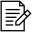
\includegraphics{./img/alg.png} Indica que el código comentado está en \textbf{lenguaje algorítmico} y es \textbf{correcto}.


\includegraphics{./img/alg_err.png} Indica que el código comentado está en \textbf{lenguaje algorítmico} y es \textbf{incorrecto}, contiene algún error.


\includegraphics{./img/c.png} Indica que el código comentado está en \textbf{lenguaje C} y es \textbf{correcto}.


\includegraphics{./img/c_err.png} Indica que el código comentado está en \textbf{lenguaje C} y es \textbf{incorrecto}, contiene algún error.

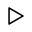
\includegraphics{./img/play.png} Muestra la ejecución de un programa en \textbf{lenguaje C}.

\hypertarget{pec01}{%
\chapter{PEC01}\label{pec01}}

\hypertarget{lenguaje-algoruxedtmico}{%
\section{Lenguaje algorítmico}\label{lenguaje-algoruxedtmico}}

El lenguaje algorítmico debemos entenderlo como una aproximación al mundo real, el cual utiliza unas normas definidas por nosotros mismos. En este punto todavía no hablamos de programas escritos en \textbf{C}, en \textbf{Java}, en \textbf{Python} o en \textbf{PHP}, por decir algunos lenguajes de programación.

Por ejemplo, en el lenguaje algorítmico que utilizamos en la asignatura definimos un bloque de variables de la siguiente forma:

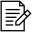
\includegraphics{./img/alg.png}

\begin{verbatim}
var
    edad: integer;
    peso: real;
end var
\end{verbatim}

Que se trate de un lenguaje más cercano al mundo real no significa que no tengan que cumplir unas determinadas reglas. Como se puede ver en este ejemplo, una de estas reglas es que cuando definimos variables lo precedente con \texttt{var} y lo finalizamos con\texttt{end\ var}.

Hemos decidido utilizar esta forma de lenguaje algorítmico, aunque también lo podríamos haber planteado de la siguiente forma:


\includegraphics{./img/alg_err.png}

\begin{verbatim}
variable
    enter edad
    decimal peso
fvariable
\end{verbatim}

Remarcar que este segundo ejemplo \textbf{es incorrecto}, no sigue la nomenclatura del lenguaje algorítmico definido en la asignatura. El correcto es el primer ejemplo.

El lenguaje algorítmico es como hacer una aproximación formal a la realidad, no es un lenguaje de programación en sí como es \textbf{C}, \textbf{Java} o similares. Por lo tanto no es un lenguaje que se pueda compilar y ejecutar con el IDE utilizado en la asignatura, el cual está preparado únicamente para interpretar y ejecutar código programado en lenguaje C.

En este punto biene la gran pregunta: ¿y por qué es necesario primero diseñar el algoritmo, si puedo directamente programarlo en C?

Un algoritmo nos permite diseñar un programa sin tener presentes las particularidades de cada lenguaje de programación. Esta aproximación formal a la realidad de los algoritmos nos facilitan poder hacer posteriormente una traducción rápida a cualquier lenguaje de programación simplemente conociendo las equivalencias correspondientes. Por ejemplo, el primer caso si lo programamos en C equivale a:


\includegraphics{./img/c.png}

\begin{Shaded}
\begin{Highlighting}[]
\DataTypeTok{int}\NormalTok{ edad;}
\DataTypeTok{float}\NormalTok{ peso;}
\end{Highlighting}
\end{Shaded}

El código en C no lo podemos cambiar, ya que si en vez de poner \texttt{int} utilizamos \texttt{entero}, el compilador de C no comprende la palabra y nos dará un error de código.

Si nunca hemos programado es normal que este planteamiento sorprenda al principio, pero es importante que poco a poco se vaya viendo las diferencias entre lenguaje algorítmico y lenguaje C.

\hypertarget{lenguaje-algoruxedtmico-vs-lenguaje-c}{%
\section{Lenguaje algorítmico vs lenguaje C}\label{lenguaje-algoruxedtmico-vs-lenguaje-c}}

En general:

\begin{itemize}
\tightlist
\item
  \textbf{Lenguaje algorítmico}: cercano al lenguaje natural, se trata de una convención que adoptamos nosotros mismos para definir el un programa formalmente. Los algoritmos tienen una serie de normas y sentencias que nosotros definimos (\textbf{Nomenclátor}), pero que no son de ninguna forma interpretables por un ordenador. Por lo tanto un algoritmo \textbf{no puede ser compilado ni ejecutado}.
\item
  \textbf{Lenguaje C}: se trata de un lenguaje de programación que sí comprende un ordenador. Esto significa que únicamente podemos utilizar sus pedidos y sus normas para que el código pueda ser compilado y ejecutado sin problemas.
\end{itemize}

El lenguaje algorítmico es un pseudocódigo que nos ayuda a definir cómo funciona un programa. No está ligado a ningún lenguaje de programación, con lo que las acciones que realizará, la forma de definir variables, etc. es genérica. Funciones como \texttt{writeString()}, \texttt{readInteger()} o \texttt{writeChar()} forman parte del lenguaje algorítmico: indican una acción genérica a realizar, como es escribir una cadena de caracteres, leer un entero o escribir un carácter. Cuando se quiera codificar este algoritmo en un lenguaje de programación concreto como es C, sólo será necesario saber los pedidos propias de C que nos permiten implementar el algoritmo.

La programación en C funciona exclusivamente con la sintaxis definida por este lenguaje de programación. Instrucciones como \texttt{scanf()} y \texttt{print\ ()} son propias de C.

A modo de ejemplo:

\textbf{Algoritmo}: queremos introducir la lectura de la luz de nuestra casa; una posible implementación es:

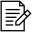
\includegraphics{./img/alg.png}

\begin{verbatim}
algorithm lecturaLuz
    var
        lecturaMensual: integer;
    end var

    writeString("Introduce la lectura mensual de la luz (kWh): ");
    lecturaMensual := readInteger();
end algorithm
\end{verbatim}

\textbf{Lenguaje C}: en este lenguaje no existen las funciones algorítmicas \texttt{writeString()} ni \texttt{readInteger()}, pero en cambio sí tenemos varias funciones propias de C que nos permiten leer un valor por teclado y asignarlo a una variable de entorno. Por tanto, las acciones algorítmicas anteriores tendrán la siguiente correspondencia en C:


\includegraphics{./img/c.png}

\begin{Shaded}
\begin{Highlighting}[]
\PreprocessorTok{\#include }\ImportTok{\textless{}stdio.h\textgreater{}}

\DataTypeTok{int}\NormalTok{ main(}\DataTypeTok{int}\NormalTok{ argc, }\DataTypeTok{char}\NormalTok{ **argv) \{ }
    \DataTypeTok{int}\NormalTok{ lecturaMensual;}

\NormalTok{    printf(}\StringTok{"Introduce la lectura mensual de la luz (kWh): "}\NormalTok{);}
\NormalTok{    scanf(}\StringTok{"\%d"}\NormalTok{, \&lecturaMensual);}
    \ControlFlowTok{return} \DecValTok{0}\NormalTok{;}
\NormalTok{\}}
\end{Highlighting}
\end{Shaded}

Es muy importante que se vea claramente qué es un \textbf{algoritmo} y que es un \textbf{programa en C}.

\hypertarget{equivalencias-lenguaje-algoruxedtmico-vs-lenguaje-c}{%
\section{Equivalencias lenguaje algorítmico vs lenguaje C}\label{equivalencias-lenguaje-algoruxedtmico-vs-lenguaje-c}}

A continuación se indican algunas de las equivalencias existentes entre lenguaje algorítmico y el lenguaje de programación C:

\begin{longtable}[]{@{}lcc@{}}
\toprule
& Lenguaje algorítmico & Lenguaje C\tabularnewline
\midrule
\endhead
Sigue unas normas? & sí & sí\tabularnewline
Se puede compilar? & no & sí\tabularnewline
Se puede ejecutar? & no & sí\tabularnewline
Asignación de valores a variables & \texttt{=} & \texttt{=}\tabularnewline
Tipo booleano & \texttt{boolean} & \texttt{bool}\tabularnewline
Tipo entero & \texttt{integer} & \texttt{int}\tabularnewline
Tipo decimal & \texttt{real} & \texttt{float}\tabularnewline
Tipo carácter & \texttt{char} & \texttt{char}\tabularnewline
Operador igual & \texttt{=} & \texttt{==}\tabularnewline
Operador diferente & \texttt{≠} & \texttt{!\ =}\tabularnewline
Operador mayor & \texttt{\textgreater{}} & \texttt{\textgreater{}}\tabularnewline
Operador mayor o igual & \texttt{≥} & \texttt{\textgreater{}\ =}\tabularnewline
Operador menor & \texttt{\textless{}} & \texttt{\textless{}}\tabularnewline
Operador menor o igual & \texttt{≤} & \texttt{\textless{}=}\tabularnewline
Operador lógico de conjunción & \texttt{and} & \texttt{\&\&}\tabularnewline
Operador lógico de disyunción & \texttt{or} & \texttt{\textbar{}\textbar{}}\tabularnewline
Operador lógico de negación & \texttt{not} & \texttt{!}\tabularnewline
\bottomrule
\end{longtable}

\hypertarget{impresiuxf3n-de-valores-incorrecta}{%
\section{Impresión de valores incorrecta}\label{impresiuxf3n-de-valores-incorrecta}}

Cuando se muestra por pantalla el contenido de alguna variable con \texttt{printf()} es importante eliminar el prefijo \texttt{\&} de la variable. Por ejemplo, si no lo hacemos tenemos que:


\includegraphics{./img/c_err.png}

\begin{Shaded}
\begin{Highlighting}[]
\PreprocessorTok{\#include }\ImportTok{\textless{}stdio.h\textgreater{}}

\DataTypeTok{int}\NormalTok{ main(}\DataTypeTok{int}\NormalTok{ argc, }\DataTypeTok{char}\NormalTok{ **argv)\{}
    \DataTypeTok{int}\NormalTok{ idAvion;}

\NormalTok{    printf(}\StringTok{"Introduce el identificador del avión : "}\NormalTok{);}
\NormalTok{    scanf(}\StringTok{"\%d"}\NormalTok{, \&idAvion);}
    
\NormalTok{    printf(}\StringTok{"\textgreater{}\textgreater{} Has elegido el avión con id \%d }\SpecialCharTok{\textbackslash{}n}\StringTok{"}\NormalTok{, \&idAvion);}
    \ControlFlowTok{return} \DecValTok{0}\NormalTok{;}
\NormalTok{\}}
\end{Highlighting}
\end{Shaded}

El resultado de la ejecución es:

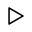
\includegraphics{./img/play.png}

\begin{Shaded}
\begin{Highlighting}[]
\NormalTok{Introduce el identificador del avión : }\DecValTok{9}
\NormalTok{\textgreater{}\textgreater{} Has elegido el avión con id {-}}\DecValTok{1078693464}
\end{Highlighting}
\end{Shaded}

¿Por qué obtenemos el valor extraño en el identificador de avión? Cuando hacemos referencia a \texttt{\&idAvion} estamos obteniendo realmente la posición de memoria donde reside la variable \texttt{idAvion}, no el valor de la variable. Para obtener su valor necesario eliminar dentro \texttt{printf()} el prefijo \texttt{\&} de la variable \texttt{idAvion}:


\includegraphics{./img/c.png}

\begin{Shaded}
\begin{Highlighting}[]
\PreprocessorTok{\#include }\ImportTok{\textless{}stdio.h\textgreater{}}

\DataTypeTok{int}\NormalTok{ main(}\DataTypeTok{int}\NormalTok{ argc, }\DataTypeTok{char}\NormalTok{ **argv)\{}
    \DataTypeTok{int}\NormalTok{ idAvion;}

\NormalTok{    printf(}\StringTok{"Introduce el identificador del avión : "}\NormalTok{);}
\NormalTok{    scanf(}\StringTok{"\%d"}\NormalTok{, \&idAvion);}
    
\NormalTok{    printf(}\StringTok{"\textgreater{}\textgreater{} Has elegido el avión con id \%d }\SpecialCharTok{\textbackslash{}n}\StringTok{"}\NormalTok{, idAvion);}
    \ControlFlowTok{return} \DecValTok{0}\NormalTok{;}
\NormalTok{\}}
\end{Highlighting}
\end{Shaded}

La salida generada ahora sí es correcta:

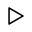
\includegraphics{./img/play.png}

\begin{Shaded}
\begin{Highlighting}[]
\NormalTok{Introduce el identificador del avión : }\DecValTok{9}
\NormalTok{\textgreater{}\textgreater{} Has elegido el avión con id }\DecValTok{9} 
\end{Highlighting}
\end{Shaded}

\hypertarget{cuxf3mo-definir-un-enumerativo}{%
\section{Cómo definir un enumerativo}\label{cuxf3mo-definir-un-enumerativo}}

La definición de un tipo enumerativo en lenguaje algorítmico se hace de la siguiente forma:

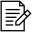
\includegraphics{./img/alg.png}

\begin{verbatim}
type
    typeName = {VALUE1, VALUE2, VALUE3, ... , VALUEn};
end type
\end{verbatim}

Los elementos \texttt{VALUE1},\texttt{VALUE2}, \texttt{VALUE3} \ldots{} acaban siendo constantes, y el valor que de cada uno es:

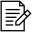
\includegraphics{./img/alg.png}

\begin{verbatim}
VALUE1 = 0
VALUE2 = 1
VALUE3 = 2 
{ ... }
VALUEn = n-1
\end{verbatim}

Posteriormente no es posible hacer un cambio de valor de estos elementos de tipo enumerativo.

\hypertarget{cuxf3mo-utilizar-un-enumerativo}{%
\section{Cómo utilizar un enumerativo}\label{cuxf3mo-utilizar-un-enumerativo}}

Una enumeración es una asignación de un valor entero a la serie de elementos que se ha definido, empezando por 0 y incrementándose en 1 en cada elemento.

Por ejemplo, podemos tener la siguiente definición:


\includegraphics{./img/c.png}

\begin{Shaded}
\begin{Highlighting}[]
\KeywordTok{typedef} \KeywordTok{enum}\NormalTok{ \{MALE, FEMALE\} tGender;}
\end{Highlighting}
\end{Shaded}

Esto significa que \texttt{MALE\ ==\ 0} y\texttt{FEMALE\ ==\ 1}. Si la orden de la definición se hubiera hecho al revés, \texttt{\{FEMALE,\ MALE\}}, tendríamos que \texttt{FEMALE\ ==\ 0} y\texttt{MALE\ ==\ 1}.

Una posible forma de utilizar los enumerativos se leer un entero y compararlo con el elemento correspondiente definido dentro del \texttt{enum}, para realizar una acción u otra. Una posible implementación en lenguaje C sería:


\includegraphics{./img/c.png}

\begin{Shaded}
\begin{Highlighting}[]
\PreprocessorTok{\#include }\ImportTok{\textless{}stdio.h\textgreater{}}

\KeywordTok{typedef} \KeywordTok{enum}\NormalTok{ \{MALE, FEMALE\} tGender;}

\DataTypeTok{int}\NormalTok{ main(}\DataTypeTok{int}\NormalTok{ argc, }\DataTypeTok{char}\NormalTok{ **argv) \{}
\NormalTok{    tGender gender;}

\NormalTok{    printf(}\StringTok{"Type patient gender: 0 for MALE, 1 for FEMALE}\SpecialCharTok{\textbackslash{}n}\StringTok{"}\NormalTok{);}
\NormalTok{    scanf(}\StringTok{"\%u"}\NormalTok{, \&gender);}

    \ControlFlowTok{if}\NormalTok{ (gender == MALE) \{}
\NormalTok{        printf(}\StringTok{"Patient gender MALE}\SpecialCharTok{\textbackslash{}n}\StringTok{"}\NormalTok{);}
\NormalTok{    \} }\ControlFlowTok{else}\NormalTok{ \{}
        \ControlFlowTok{if}\NormalTok{ (gender == FEMALE) \{}
\NormalTok{            printf(}\StringTok{"Patient gender FEMALE}\SpecialCharTok{\textbackslash{}n}\StringTok{"}\NormalTok{);}
\NormalTok{        \} }\ControlFlowTok{else}\NormalTok{ \{}
\NormalTok{            printf(}\StringTok{"Incorrect option}\SpecialCharTok{\textbackslash{}n}\StringTok{"}\NormalTok{);}
\NormalTok{        \}}
\NormalTok{    \}}
    \ControlFlowTok{return} \DecValTok{0}\NormalTok{;}
\NormalTok{\}}
\end{Highlighting}
\end{Shaded}

\hypertarget{especificador-de-un-enumerativo}{%
\section{Especificador de un enumerativo}\label{especificador-de-un-enumerativo}}

Los enumerativos en lenguaje C, \texttt{enum} utilizan el especificador \texttt{\%u}.

Ejemplo:


\includegraphics{./img/c.png}

\begin{Shaded}
\begin{Highlighting}[]
\PreprocessorTok{\#include }\ImportTok{\textless{}stdio.h\textgreater{}}

\KeywordTok{typedef} \KeywordTok{enum}\NormalTok{ \{PRIVAT, PUBLIC\} tTransporte;}

\DataTypeTok{int}\NormalTok{ main(}\DataTypeTok{int}\NormalTok{ argc, }\DataTypeTok{char}\NormalTok{ **argv) \{}
\NormalTok{    tTransporte tipoTransporte;}

\NormalTok{    printf(}\StringTok{"¿Con qué tipo de transporte te desplazas al trabajo (0 = privado, 1 = público)?:"}\NormalTok{);}
\NormalTok{    scanf(}\StringTok{"\%u"}\NormalTok{, \&tipoTransporte);}
\NormalTok{    printf(}\StringTok{"Te desplazas al trabajo en transporte (0 = privado, 1 = público):"}\NormalTok{);}
\NormalTok{    printf(}\StringTok{"\%u}\SpecialCharTok{\textbackslash{}n}\StringTok{"}\NormalTok{, tipoTransporte);}
    \ControlFlowTok{return} \DecValTok{0}\NormalTok{;}
\NormalTok{\}}
\end{Highlighting}
\end{Shaded}

\hypertarget{lectura-de-caracteres-en-c}{%
\section{Lectura de caracteres en C}\label{lectura-de-caracteres-en-c}}

En el lenguaje C la lectura de un \texttt{char} puede comportarse de forma inadecuada si previamente el buffer de entrada contiene algún carácter previo.

Imaginemos que queremos crear un programa muy sencillo que dado un número de DNI y su letra, nos concatenar los dos valores y lo muestre por pantalla. Una posible forma de implementar este programa en C sería:


\includegraphics{./img/c_err.png}

\begin{Shaded}
\begin{Highlighting}[]
\PreprocessorTok{\#include }\ImportTok{\textless{}stdio.h\textgreater{}}

\DataTypeTok{int}\NormalTok{ main(}\DataTypeTok{int}\NormalTok{ argc, }\DataTypeTok{char}\NormalTok{ **argv) \{}
    \DataTypeTok{int}\NormalTok{ dniNum;    }\CommentTok{/* número del DNI */}
    \DataTypeTok{char}\NormalTok{ dniChar;  }\CommentTok{/* letra del DNI */}

\NormalTok{    printf(}\StringTok{"Introduce el número del DNI: "}\NormalTok{);}
\NormalTok{    scanf(}\StringTok{"\%d"}\NormalTok{, \&dniNum);}
\NormalTok{    printf(}\StringTok{"Introduce la letra del DNI: "}\NormalTok{);}
\NormalTok{    scanf(}\StringTok{"\%c"}\NormalTok{, \&dniChar);}

\NormalTok{    printf(}\StringTok{"}\SpecialCharTok{\textbackslash{}n}\StringTok{El DNI introducido es: \%d{-}\%c}\SpecialCharTok{\textbackslash{}n}\StringTok{"}\NormalTok{, dniNum, dniChar);}
    \ControlFlowTok{return} \DecValTok{0}\NormalTok{;}
\NormalTok{\}}
\end{Highlighting}
\end{Shaded}

¿Qué pasa si ejecutamos este código? Que vemos que se comporta de forma incorrecta, ya que no nos llega a pedir la letra del DNI, mostrando directamente el resultado:

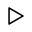
\includegraphics{./img/play.png}

\begin{Shaded}
\begin{Highlighting}[]
\NormalTok{Introduce el número del DNI: }\DecValTok{12345678}
\NormalTok{Introduce la letra del DNI:}
\NormalTok{El DNI introducido es: }\DecValTok{12345678}\NormalTok{{-}}
\end{Highlighting}
\end{Shaded}

Cuando tecleamos el primer entero lo que hacemos realmente es introducir un número + un \texttt{intro} al final de todo. El número queda asignado a la variable \texttt{dni\_num}, y el\texttt{intro} es leído como un carácter y se asigna a la variable \texttt{dni\_char}. Por este motivo C interpreta que las dos variables ya tienen valor y finaliza el programa.

Como podemos solucionar este comportamiento? Vaciando el \texttt{intro} del buffer de entrada antes de leer el carácter, y una posible forma de hacerlo es mediante el comando \texttt{getchar()}. Este comando lee un carácter del buffer de entrada y el vacío del buffer.

Por lo tanto se puede corregir el programa anterior de la siguiente forma:


\includegraphics{./img/c.png}

\begin{Shaded}
\begin{Highlighting}[]
\PreprocessorTok{\#include }\ImportTok{\textless{}stdio.h\textgreater{}}

\DataTypeTok{int}\NormalTok{ main(}\DataTypeTok{int}\NormalTok{ argc, }\DataTypeTok{char}\NormalTok{ **argv) \{}
    \DataTypeTok{int}\NormalTok{ dni\_num;    }\CommentTok{/* número del DNI */}
    \DataTypeTok{char}\NormalTok{ dni\_char;  }\CommentTok{/* letra del DNI */}

\NormalTok{    printf(}\StringTok{"Introduce el número del DNI: "}\NormalTok{);}
\NormalTok{    scanf(}\StringTok{"\%d"}\NormalTok{, \&dni\_num);}
\NormalTok{    getchar();}
\NormalTok{    printf(}\StringTok{"Introduce la letra del DNI: "}\NormalTok{);}
\NormalTok{    scanf(}\StringTok{"\%c"}\NormalTok{, \&dni\_char);}

\NormalTok{    printf(}\StringTok{"}\SpecialCharTok{\textbackslash{}n}\StringTok{El DNI introducido es: \%d{-}\%c}\SpecialCharTok{\textbackslash{}n}\StringTok{"}\NormalTok{, dni\_num, dni\_char);}
    \ControlFlowTok{return} \DecValTok{0}\NormalTok{;}
\NormalTok{\}}
\end{Highlighting}
\end{Shaded}

Si ahora ejecutamos ya funcionará como deseamos:

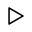
\includegraphics{./img/play.png}

\begin{Shaded}
\begin{Highlighting}[]
\NormalTok{Introduce el número del DNI: }\DecValTok{12345678}
\NormalTok{Introduce la letra del DNI: B}

\NormalTok{El DNI introducido es: }\DecValTok{12345678}\NormalTok{{-}B}
\end{Highlighting}
\end{Shaded}

En caso de necesidad, con \texttt{getchar()} se puede guardar el carácter del buffer en una variable para tratarlo posteriormente:


\includegraphics{./img/c.png}

\begin{Shaded}
\begin{Highlighting}[]
\DataTypeTok{char}\NormalTok{ nombreVariable;}
\NormalTok{nombreVariable = getChar();}
\end{Highlighting}
\end{Shaded}

\hypertarget{lectura-de-float-en-c}{%
\section{Lectura de float en C}\label{lectura-de-float-en-c}}

El separador de valores decimales (tipo \texttt{float}) en C \textbf{es el punto}, no la coma. De ahí que cuando se introduce un valor decimal desde teclado siempre lo haremos con un punto:

Ejemplo:


\includegraphics{./img/c.png}

\begin{Shaded}
\begin{Highlighting}[]
\PreprocessorTok{\#include }\ImportTok{\textless{}stdio.h\textgreater{}}

\DataTypeTok{int}\NormalTok{ main(}\DataTypeTok{int}\NormalTok{ argc, }\DataTypeTok{char}\NormalTok{ **argv) \{\}}
    \CommentTok{/* Variable que contendrá el peso de una persona */}
    \DataTypeTok{float}\NormalTok{ peso;}

    \CommentTok{/* Lectura del dato por teclado (el separador decimal es un . ) */}
\NormalTok{    printf(}\StringTok{"Introduce el peso (kg) de una persona : "}\NormalTok{);}
\NormalTok{    scanf(}\StringTok{"\%f"}\NormalTok{, \&peso);}

    \CommentTok{/* Se muestra el valor decimal por pantalla */}
\NormalTok{    printf(}\StringTok{"Has introducido el peso = \%.1f kg.}\SpecialCharTok{\textbackslash{}n}\StringTok{"}\NormalTok{, peso);}
    \ControlFlowTok{return} \DecValTok{0}\NormalTok{;}
\NormalTok{\}}
\end{Highlighting}
\end{Shaded}

La ejecución será:

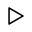
\includegraphics{./img/play.png}

\begin{Shaded}
\begin{Highlighting}[]
\NormalTok{Introduce el peso (kg) de una persona : }\FloatTok{79.440}
\NormalTok{Has introducido el peso = }\FloatTok{79.4}\NormalTok{ kg.}
\end{Highlighting}
\end{Shaded}

\hypertarget{frequently-made-mistakes}{%
\section{Frequently Made Mistakes}\label{frequently-made-mistakes}}

\hypertarget{definiciuxf3n-de-tipos-tipo-booleano}{%
\subsection{Definición de tipos: tipo booleano}\label{definiciuxf3n-de-tipos-tipo-booleano}}

En lenguaje algorítmico, el tipo \texttt{boolean} es un tipo básico, y como tal no es necesario definirlo en un bloque \texttt{type}.

Pseudocódigo incorrecto:


\includegraphics{./img/alg_err.png}

\begin{verbatim}
type
    boolean = {FALSE, TRUE};
type
var 
    myNum: integer;
    myBool: boolean;
end var
\end{verbatim}

Se pueden declarar variables de tipo booleano directamente, al igual que si fuera un entero, un real o un carácter.

Pseudocódigo correcto:

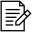
\includegraphics{./img/alg.png}

\begin{verbatim}
var 
    myNum: integer;
    myBool: boolean;
end var
\end{verbatim}

\hypertarget{estilo-y-formato-ausencia-de-estilo-y-formato-en-lenguaje-algoruxedtmico}{%
\subsection{Estilo y formato: ausencia de estilo y formato en lenguaje algorítmico}\label{estilo-y-formato-ausencia-de-estilo-y-formato-en-lenguaje-algoruxedtmico}}

Este no es un error sintáctico o semántico, sino una mala práctica de diseño y programación muy frecuente.

Pseudocódigo incorrecto:


\includegraphics{./img/alg_err.png}

\begin{verbatim}
action readHotel(out room: integer, out price: real)
var
i: integer;
end var
writeString("Enter room:");
readInteger(room);
writeString("Enter price:");
readReal(totalPrice);
if(price>MAXPRICE) then
writeString("Invalid price");
end if
for i=1 to rooms do
writeString("Room: ");
writeInteger(i);
end for
end action
\end{verbatim}

En el caso del lenguaje algorítmico, las reglas de formato y de estilo son arbitrarias y fijadas por convenio, pero hay que seguir para que sea fácil de leer y revisar, de la misma forma que se hace cuando se programa en C u otros lenguajes. En el ejemplo anterior, no hay aplicada ninguna indentación y el pseudocódigo es muy difícil de leer. Fijaos cómo cambia cuando aplicamos correctamente unas mínimas reglas.

Pseudocódigo correcto:

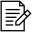
\includegraphics{./img/alg.png}

\begin{Shaded}
\begin{Highlighting}[]
\NormalTok{action readHotel(out room: }\DataTypeTok{integer}\NormalTok{, out price: }\DataTypeTok{real}\NormalTok{)}
    \KeywordTok{var}
\NormalTok{        i: }\DataTypeTok{integer}\NormalTok{;}
    \KeywordTok{end} \KeywordTok{var}
    
\NormalTok{    writeString("Enter room:");}
\NormalTok{    readInteger(room);}
\NormalTok{    writeString("Enter price:");}
\NormalTok{    readReal(totalPrice);}
    
    \KeywordTok{if}\NormalTok{ (price \textgreater{} MAXPRICE) }\KeywordTok{then}
\NormalTok{        writeString("Invalid price");}
    \KeywordTok{end} \KeywordTok{if}
    
    \KeywordTok{for}\NormalTok{ i:=}\DecValTok{1} \KeywordTok{to}\NormalTok{ rooms }\KeywordTok{do}
\NormalTok{        writeString("Room: ");}
\NormalTok{    writeInteger(i);}
    \KeywordTok{end} \KeywordTok{for}
\KeywordTok{end}\NormalTok{ action}
\end{Highlighting}
\end{Shaded}

Cabe mencionar que el \textbf{sangrado} del texto (tabulaciones) es especialmente importante para la lectura de los programas, ya que permiten identificar rápidamente los bloques de código, las funciones y acciones, las estructuras iterativas y alternativas, y su dependencia jerárquica. Por este motivo, el uso de sangrado en el pseudocódigo es absolutamente necesario.

\hypertarget{declaraciuxf3n-de-variables-identificadores-no-permitidos}{%
\subsection{Declaración de variables: identificadores no permitidos}\label{declaraciuxf3n-de-variables-identificadores-no-permitidos}}

Pseudocódigo incorrecto:


\includegraphics{./img/alg_err.png}

\begin{verbatim}
var
    1Hotel_ID: integer;
    2Hotel_ID: integer;
end var
\end{verbatim}

El nombre de las variables puede contener números siempre que no estén en la primera posición. Utilizaremos el modelo \href{https://en.wikipedia.org/wiki/Camel_case}{camelCase} para definir el nombre de las variables.

Pseudocódigo correcto:

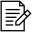
\includegraphics{./img/alg.png}

\begin{verbatim}
var
    hotelId1: integer;
    hotelId2: integer;
end var
\end{verbatim}

\hypertarget{declaraciuxf3n-de-variables-operador-de-declaraciuxf3n}{%
\subsection{Declaración de variables: operador de declaración}\label{declaraciuxf3n-de-variables-operador-de-declaraciuxf3n}}

Pseudocódigo incorrecto:


\includegraphics{./img/alg_err.png}

\begin{verbatim}
var
    id:= integer;
    brand:= string;
    name:= string;
end var
\end{verbatim}

El siguiente error podría parecer un error leve, pero es importante respetar el \textbf{Nomenclátor} y utilizar los operadores correctamente. En lenguaje algorítmico, el operador de declaración de tipo es \texttt{:} y no \texttt{=}, que es el operador de asignación de valor.

Pseudocódigo correcto:

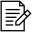
\includegraphics{./img/alg.png}

\begin{verbatim}
var
    id: integer;
    brand: string;
    name: string;
end var
\end{verbatim}

\hypertarget{pec02}{%
\chapter{PEC02}\label{pec02}}

\hypertarget{booleanos-en-c}{%
\section{Booleanos en C}\label{booleanos-en-c}}

Algunos puntos a considerar con los booleanos en C:

\begin{itemize}
\tightlist
\item
  Cuando utilizamos el tipo \texttt{bool} de C necesitamos importar la librería \texttt{\textless{}stdbool.h\textgreater{}}, ya que el tipo\texttt{bool} no se definió a las primeras versiones del lenguaje C.
\item
  Los valores que puede tomar una variable booleana en C son \texttt{false} y\texttt{true}. El lenguaje C trata internamente estos valores como enteros: \texttt{false} corresponde a \texttt{0} y \texttt{true} a \texttt{1}.
\item
  Cuando queramos introducir el valor de un booleano para teclado o bien mostrarlo por pantalla, utilizaremos el entero \texttt{0} para referirnos a \texttt{false} y \texttt{1} por \texttt{true}.
\item
  El especificador de tipo de los booleanos es \texttt{\%d}.
\item
  Para mostrar el valor de una variable booleana en C lo podemos hacer de la siguiente forma:

  
\includegraphics{./img/c.png}
\end{itemize}

\begin{Shaded}
\begin{Highlighting}[]
\DataTypeTok{bool}\NormalTok{ isVocal;}
\NormalTok{printf(}\StringTok{"La letra \%c es una vocal (0=false, 1=true) ? \%d}\SpecialCharTok{\textbackslash{}n}\StringTok{"}\NormalTok{, letra, isVocal);}
\end{Highlighting}
\end{Shaded}

\begin{itemize}
\tightlist
\item
  Para leer un booleano desde teclado, lo haríamos de la siguiente forma:

  
\includegraphics{./img/c.png}
\end{itemize}

\begin{Shaded}
\begin{Highlighting}[]
\DataTypeTok{bool}\NormalTok{ variable;}
\NormalTok{scanf(}\StringTok{"\%d"}\NormalTok{, \&variable);}
\end{Highlighting}
\end{Shaded}

\begin{itemize}
\tightlist
\item
  La lectura para teclado de un booleano, hecha como se indica en el punto anterior, generará un \emph{warning} del siguiente tipo: \texttt{warning:\ formato\ \textquotesingle{}\%\ de\ expects\ argumento\ of\ type\textquotesingle{}\ int\ *\ \textquotesingle{},\ but\ argumento\ 2\ has\ type\ \textquotesingle{}\_Bool\ *\textquotesingle{}\ {[}-Wformat\ ={]}}. Este aviso significa que estamos utilizando un especificador de tipo (\texttt{\%d}) distinto del que le correspondería al tipo \texttt{bool}, el cual trabaja únicamente con 1 bit. Como C no dispone de ningún especificador de tipo que trabaje sólo con 1 bit, podemos hacer dos cosas:

  \begin{itemize}
  \tightlist
  \item
    Utilizar una variable auxiliar que nos ayude a hacer una conversión intermedia a \texttt{int}, a fin de transformar posteriormente el valor a \texttt{bool}:

    
\includegraphics{./img/c.png}
  \end{itemize}

\begin{Shaded}
\begin{Highlighting}[]
\DataTypeTok{bool}\NormalTok{ variable;}
\DataTypeTok{int}\NormalTok{ aux;}
\NormalTok{scanf(}\StringTok{"\%d"}\NormalTok{, \&aux);}
\NormalTok{variable = aux;}
\end{Highlighting}
\end{Shaded}

  \begin{itemize}
  \tightlist
  \item
    Ignorar el warning de esta situación específica: a pesar del aviso, el programa se puede compilar y ejecutar.
  \end{itemize}
\end{itemize}

\hypertarget{booleanos-definidos-como-enumerativos}{%
\section{Booleanos definidos como enumerativos}\label{booleanos-definidos-como-enumerativos}}

En semestres anteriores de la asignatura de \textbf{Fundamentos de Programación}, se utilizaba un \textbf{enumerativo} para definir el tipo booleano:


\includegraphics{./img/c.png}

\begin{Shaded}
\begin{Highlighting}[]
\KeywordTok{typedef} \KeywordTok{enum}\NormalTok{ \{FALSE, TRUE\} boolean;}
\end{Highlighting}
\end{Shaded}

Esta forma de definir el tipo booleano es \textbf{obsoleta} y \textbf{no utiliza} este semestre; tal y como se ha comentado en el apartado \protect\hyperlink{booleanos-en-c}{Booleanos en C}, los booleanos los definiremos mediante la librería \texttt{\textless{}stdbool.h\textgreater{}}. Tenedlo presente cuando consulte PAC\footnote{PAC: Prueba de Evaluación Continua}, PR\footnote{PR: Práctica} y PS\footnote{PS: Prueba de Síntesis} de semestres anteriores, en los que se utilizaba la nomenclatura ahora obsoleta.

\hypertarget{constantes-define-vs-const}{%
\section{Constantes: define vs const}\label{constantes-define-vs-const}}

La definición de constantes se puede hacer tanto con \texttt{define} como con \texttt{const}. Sin embargo, la forma de comportarse de estas dos opciones es completamente diferente, aunque el resultado final acabe siendo el mismo:

\begin{itemize}
\tightlist
\item
  \texttt{define}: cuando utilizamos esta opción no se guarda en ninguna posición de memoria el valor de la constante. Lo que se hace realmente es que en los pasos previos a la propia compilación del programa, el preprocesador sustituye todas las referencias del define por el valor indicado.
\end{itemize}

Por ejemplo, si tenemos el siguiente programa con una constante creada con \texttt{define}:


\includegraphics{./img/c.png}

\begin{Shaded}
\begin{Highlighting}[]
\PreprocessorTok{\#include }\ImportTok{\textless{}stdio.h\textgreater{}}
\PreprocessorTok{\#define MEDIDA 8}

\DataTypeTok{char}\NormalTok{ letras[] = \{}\CharTok{\textquotesingle{}a\textquotesingle{}}\NormalTok{, }\CharTok{\textquotesingle{}b\textquotesingle{}}\NormalTok{, }\CharTok{\textquotesingle{}c\textquotesingle{}}\NormalTok{, }\CharTok{\textquotesingle{}d\textquotesingle{}}\NormalTok{, }\CharTok{\textquotesingle{}e\textquotesingle{}}\NormalTok{, }\CharTok{\textquotesingle{}f\textquotesingle{}}\NormalTok{, }\CharTok{\textquotesingle{}g\textquotesingle{}}\NormalTok{, }\CharTok{\textquotesingle{}h\textquotesingle{}}\NormalTok{\};}
\DataTypeTok{int}\NormalTok{ vertical, horizontal;}

\DataTypeTok{int}\NormalTok{ main(}\DataTypeTok{int}\NormalTok{ argc, }\DataTypeTok{char}\NormalTok{ **argv) \{}
    \CommentTok{/* fuente: https://en.wikipedia.org/wiki/Chess */}
    \ControlFlowTok{for}\NormalTok{ (vertical=MEDIDA; vertical\textgreater{}=}\DecValTok{1}\NormalTok{; vertical{-}{-}) \{}
        \ControlFlowTok{for}\NormalTok{ (horizontal=}\DecValTok{0}\NormalTok{; horizontal\textless{}=MEDIDA{-}}\DecValTok{1}\NormalTok{; horizontal++) \{}
\NormalTok{            printf(}\StringTok{"\%c\%d "}\NormalTok{, letras[horizontal], vertical);}
\NormalTok{        \}}
\NormalTok{        printf(}\StringTok{"}\SpecialCharTok{\textbackslash{}n}\StringTok{"}\NormalTok{);}
\NormalTok{    \}}
    \ControlFlowTok{return} \DecValTok{0}\NormalTok{;}
\NormalTok{\}}
\end{Highlighting}
\end{Shaded}

Antes de la compilación, el preprocesador entre otras acciones elimina comentarios y sustituye todas las referencias \texttt{MEDIDA} por \texttt{8}:


\includegraphics{./img/c.png}

\begin{Shaded}
\begin{Highlighting}[]
\PreprocessorTok{\#include }\ImportTok{\textless{}stdio.h\textgreater{}}

\DataTypeTok{char}\NormalTok{ letras[] = \{}\CharTok{\textquotesingle{}a\textquotesingle{}}\NormalTok{, }\CharTok{\textquotesingle{}b\textquotesingle{}}\NormalTok{, }\CharTok{\textquotesingle{}c\textquotesingle{}}\NormalTok{, }\CharTok{\textquotesingle{}d\textquotesingle{}}\NormalTok{, }\CharTok{\textquotesingle{}e\textquotesingle{}}\NormalTok{, }\CharTok{\textquotesingle{}f\textquotesingle{}}\NormalTok{, }\CharTok{\textquotesingle{}g\textquotesingle{}}\NormalTok{, }\CharTok{\textquotesingle{}h\textquotesingle{}}\NormalTok{\};}
\DataTypeTok{int}\NormalTok{ vertical, horizontal;}

\DataTypeTok{int}\NormalTok{ main(}\DataTypeTok{int}\NormalTok{ argc, }\DataTypeTok{char}\NormalTok{ **argv) \{}
    \ControlFlowTok{for}\NormalTok{ (vertical=}\DecValTok{8}\NormalTok{; vertical\textgreater{}=}\DecValTok{1}\NormalTok{; vertical{-}{-}) \{}
        \ControlFlowTok{for}\NormalTok{ (horizontal=}\DecValTok{0}\NormalTok{; horizontal\textless{}=}\DecValTok{8}\NormalTok{{-}}\DecValTok{1}\NormalTok{; horizontal++) \{}
\NormalTok{            printf(}\StringTok{"\%c\%d "}\NormalTok{, letras[horizontal], vertical);}
\NormalTok{        \}}
\NormalTok{        printf(}\StringTok{"}\SpecialCharTok{\textbackslash{}n}\StringTok{"}\NormalTok{);}
\NormalTok{    \}}
    \ControlFlowTok{return} \DecValTok{0}\NormalTok{;}
\NormalTok{\}}
\end{Highlighting}
\end{Shaded}

Por lo tanto la definición de constantes con \texttt{define} se comporta como si se tratara de un \emph{``buscar-reemplazar''} de un procesador de textos. No se guarda ninguna constante en memoria, pero por el contrario, el programa ocupará un poco más para la sustitución directa de referencias que hace; la sustitución la hace en todo el programa, no se puede limitar a un ámbito concreto (por ejemplo sólo dentro de una función).

\begin{itemize}
\tightlist
\item
  \texttt{const}: en este caso sí que se reserva una posición de memoria. En C se comporta igual como si fuera una variable, pero la que únicamente funciona en modo lectura: no le podemos modificar el valor.
\end{itemize}

Además, \texttt{const} nos permite también decir qué tipo de valor tendrá la constante: si es de tipo \texttt{float}, \texttt{int},\texttt{char}\ldots{} con lo que este hecho nos da un punto adicional de control, ya que nos aseguramos de que el tipo de valor asignado será el correcto para el programa.

Con este tipo de definición de constante, el ejemplo anterior quedaría de la siguiente forma:


\includegraphics{./img/c.png}

\begin{Shaded}
\begin{Highlighting}[]
\PreprocessorTok{\#include }\ImportTok{\textless{}stdio.h\textgreater{}}
\DataTypeTok{const} \DataTypeTok{int}\NormalTok{ MEDIDA }\DecValTok{8}

\DataTypeTok{char}\NormalTok{ letras[] = \{}\CharTok{\textquotesingle{}a\textquotesingle{}}\NormalTok{, }\CharTok{\textquotesingle{}b\textquotesingle{}}\NormalTok{, }\CharTok{\textquotesingle{}c\textquotesingle{}}\NormalTok{, }\CharTok{\textquotesingle{}d\textquotesingle{}}\NormalTok{, }\CharTok{\textquotesingle{}e\textquotesingle{}}\NormalTok{, }\CharTok{\textquotesingle{}f\textquotesingle{}}\NormalTok{, }\CharTok{\textquotesingle{}g\textquotesingle{}}\NormalTok{, }\CharTok{\textquotesingle{}h\textquotesingle{}}\NormalTok{\};}
\DataTypeTok{int}\NormalTok{ vertical, horizontal;}

\DataTypeTok{int}\NormalTok{ main(}\DataTypeTok{int}\NormalTok{ argc, }\DataTypeTok{char}\NormalTok{ **argv) \{}
    \CommentTok{/* La constante MEDIDA está guardada en memòria */}
\NormalTok{    printf(}\StringTok{"posición en memoria de la constante MEDIDA : \%p }\SpecialCharTok{\textbackslash{}n}\StringTok{"}\NormalTok{, \&MEDIDA);}
    \ControlFlowTok{for}\NormalTok{ (vertical=MEDIDA; vertical\textgreater{}=}\DecValTok{1}\NormalTok{; vertical{-}{-}) \{}
        \ControlFlowTok{for}\NormalTok{ (horizontal=}\DecValTok{0}\NormalTok{; horizontal\textless{}=MEDIDA{-}}\DecValTok{1}\NormalTok{; horizontal++) \{}
\NormalTok{            printf(}\StringTok{"\%c\%d "}\NormalTok{, letras[horizontal], vertical);}
\NormalTok{        \}}
\NormalTok{        printf(}\StringTok{"}\SpecialCharTok{\textbackslash{}n}\StringTok{"}\NormalTok{);}
\NormalTok{    \}}
    \ControlFlowTok{return} \DecValTok{0}\NormalTok{;}
\NormalTok{\}}
\end{Highlighting}
\end{Shaded}

Como se puede ver, es posible obte la dirección en memoria donde se guarda la constante \texttt{MEDIDA}. En este caso, sí que puedes definir una constante con \texttt{const} y hacer que sólo afecte a un ámbito determinado (por ejemplo, que la constante esté definida únicamente dentro de una función).

Estas son las principales diferencias entre \texttt{define} y \texttt{const} a la hora de definir una constante; \texttt{define} se creó mucho antes que no la sentencia \texttt{const}, con lo que es bastante habitual decantarse por esta opción por temas históricos.

\hypertarget{cuxf3mo-mostrar-el-valor-de-una-constante}{%
\section{Cómo mostrar el valor de una constante}\label{cuxf3mo-mostrar-el-valor-de-una-constante}}

En C podemos mostrar por pantalla el valor de una constante definida con \texttt{\#define} mediante \texttt{printf()}. ejemplo:


\includegraphics{./img/c.png}

\begin{Shaded}
\begin{Highlighting}[]
\PreprocessorTok{\#include }\ImportTok{\textless{}stdio.h\textgreater{}}

\PreprocessorTok{\#define WORD "world"}
\PreprocessorTok{\#define YEAR 2021}
\PreprocessorTok{\#define EXCLAMATION \textquotesingle{}!\textquotesingle{}}

\DataTypeTok{int}\NormalTok{ main(}\DataTypeTok{int}\NormalTok{ argc, }\DataTypeTok{char}\NormalTok{ **argv) \{}
\NormalTok{    printf(}\StringTok{"hello \%s and happy \%d \%c}\SpecialCharTok{\textbackslash{}n}\StringTok{"}\NormalTok{, PALABRA, YEAR, EXCLAMATION);}
    \ControlFlowTok{return} \DecValTok{0}\NormalTok{;}
\NormalTok{\}}
\end{Highlighting}
\end{Shaded}

El resultado que se mostrará por pantalla será:

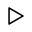
\includegraphics{./img/play.png}

\begin{Shaded}
\begin{Highlighting}[]
\NormalTok{hello world and happy }\DecValTok{2021}\NormalTok{ !}
\end{Highlighting}
\end{Shaded}

\hypertarget{precisiuxf3n-en-variables-float}{%
\section{Precisión en variables float}\label{precisiuxf3n-en-variables-float}}

Hay algunos valores decimales determinados que no se pueden representar de forma precisa en una variable de tipo \texttt{float}. La mejor solución para los casos que tratamos es redondear al número de decimales que realmente necesitamos.

Si en cambio queremos sí o sí trabajar con todos los decimales, podemos optar por utilizar un tipo de dato que tenga mayor precisión que \texttt{float}: \texttt{double}.

Por ejemplo, el siguiente programa devuelve el resultado esperado si se guarda en un \texttt{double}, y no así si se hace en un \texttt{float}:


\includegraphics{./img/c.png}

\begin{Shaded}
\begin{Highlighting}[]
\PreprocessorTok{\#include }\ImportTok{\textless{}stdio.h\textgreater{}}

\DataTypeTok{int}\NormalTok{ main(}\DataTypeTok{int}\NormalTok{ argc, }\DataTypeTok{char}\NormalTok{ **argv) \{ }
    \DataTypeTok{float}\NormalTok{ num1; }
    \DataTypeTok{float}\NormalTok{ num2;}
    \DataTypeTok{float}\NormalTok{ resultado1; }
    \DataTypeTok{double}\NormalTok{ resultado2; }
    
\NormalTok{    num1 = }\FloatTok{1.3}\NormalTok{; }
\NormalTok{    num2 = }\DecValTok{17}\NormalTok{;}
\NormalTok{    resultado1 = num1 + num2; }
\NormalTok{    printf(}\StringTok{"resultado con float : \%f}\SpecialCharTok{\textbackslash{}n}\StringTok{"}\NormalTok{, resultado1); }
\NormalTok{    resultado2 = num1 + num2; }
\NormalTok{    printf(}\StringTok{"resultado con double: \%f}\SpecialCharTok{\textbackslash{}n}\StringTok{"}\NormalTok{, resultado2); }
    \ControlFlowTok{return} \DecValTok{0}\NormalTok{; }
\NormalTok{\}}
\end{Highlighting}
\end{Shaded}

La salida generada es:

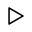
\includegraphics{./img/play.png}

\begin{Shaded}
\begin{Highlighting}[]
\NormalTok{resultado con }\DataTypeTok{float}\NormalTok{ : }\FloatTok{18.299999}
\NormalTok{resultado con }\DataTypeTok{double}\NormalTok{: }\FloatTok{18.300000}
\end{Highlighting}
\end{Shaded}

\hypertarget{semuxe1ntica-de-una-expresiuxf3n}{%
\section{Semántica de una expresión}\label{semuxe1ntica-de-una-expresiuxf3n}}

Si recordamos lo que se comenta en el punto \textbf{3.2. Semántica de una expresión} del módulo de la XWiki \textbf{Tipos básicos de datos}, tenemos que conseguir que las expresiones y comparaciones realizadas a los algoritmos sean \textbf{semánticamente correctas}.

Con un ejemplo se verá más claro: tenemos el siguiente algoritmo que indica si una persona es mayor de edad. Fijaos que la expresión realiza una comparación entre dos enteros: la variable \texttt{edad} y el número \texttt{17}.

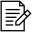
\includegraphics{./img/alg.png}

\begin{verbatim}
var
    edad: int;
    isMayorEdad: boolean;
end var

algorithm serMayorEdad

    writeString("Introduce edad del conductor :");
    edad := readInteger();

    isMayorEdad := (edad > 17);

    writeString("El conductor es mayor de edad? :");
    writeBoolean(isMayorEdad);

end algorithm
\end{verbatim}

Esta expresión \textbf{es semánticamente correcta}.

En cambio, imaginemos ahora que nuestro algoritmo acepta decimales por la \texttt{edad}; por ejemplo, \texttt{19.5} indicaría que la edad es de 19 años y 6 meses. Así tenemos el siguiente planteamiento, donde ahora la variable \texttt{edad} es de tipo \texttt{real}:

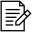
\includegraphics{./img/alg.png}

\begin{verbatim}
var
    edad: real;
    isMayorEdad: boolean;
end var

algorithm serMayorEdad

    writeString("Introduce edad del conductor :");
    edad := readReal();

    isMayorEdad := (edad > 17);

    writeString("El conductor es mayor de edad? :");
    writeBoolean(isMayorEdad);

end algorithm
\end{verbatim}

El algoritmo ahora \textbf{no es correcto} ya que contiene una expresión \textbf{semánticamente incorrecta}, en la que se compara \texttt{edad} (real) con\texttt{17} (entero). Para solucionarlo, podemos utilizar alguna de las funciones de conversión comentadas en el apartado \textbf{4. Funciones de conversión de tipos del mismo módulo}:

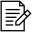
\includegraphics{./img/alg.png}

\begin{verbatim}
{ opción 1: hacemos que ambos valores sean de tipo entero }
isMayorEdad: = (realToInteger(edad) > 17);

{ opción 2: hacemos que ambos valores sean de tipo real }
isMayorEdad: = (edad > integerToReal(17));
\end{verbatim}

\hypertarget{ejemplos-de-expresiones}{%
\section{Ejemplos de expresiones}\label{ejemplos-de-expresiones}}

\hypertarget{ejemplo-1-espar}{%
\subsection{Ejemplo 1: esPar}\label{ejemplo-1-espar}}

Imaginemos que nos piden un algoritmo que indique si un número es par.

Una posible solución sería:

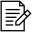
\includegraphics{./img/alg.png}

\begin{verbatim}
algorithm esPar
    var
        numero: integer;
        isPar: boolean;
    end var

    writeString("Introduce un número : ");
    numero:= readInteger();
    isPar:= (numero mod 2 = 0);
    
    writeString("El número ");
    writeInteger(numero);
    writeString(" es par? ");
    writeBoolean(isPar);

end algorithm
\end{verbatim}

La variable \texttt{isPar} tomará el valor \texttt{TRUE} si el número es par y \texttt{FALSE} lo contrario. No ha sido necesario utilizar ninguna estructura \texttt{if-else} para resolver el algoritmo.

Una posible forma de codificar en lenguaje C es:


\includegraphics{./img/c.png}

\begin{Shaded}
\begin{Highlighting}[]
\PreprocessorTok{\#include }\ImportTok{\textless{}stdio.h\textgreater{}}
\PreprocessorTok{\#include }\ImportTok{\textless{}stdbool.h\textgreater{}}

\DataTypeTok{int}\NormalTok{ main(}\DataTypeTok{int}\NormalTok{ argc, }\DataTypeTok{char}\NormalTok{ **argv) \{}
    \DataTypeTok{int}\NormalTok{ numero;}
    \DataTypeTok{bool}\NormalTok{ isPar;}

\NormalTok{    printf(}\StringTok{"Introduce un número : "}\NormalTok{);}
\NormalTok{    scanf(}\StringTok{"\%d"}\NormalTok{, \&numero);}
\NormalTok{    isPar = (numero \% }\DecValTok{2}\NormalTok{ == }\DecValTok{0}\NormalTok{);}
    
\NormalTok{    printf(}\StringTok{"El número \%d es par? (0=FALSE, 1=TRUE) : \%d }\SpecialCharTok{\textbackslash{}n}\StringTok{"}\NormalTok{, numero, isPar);}
    \ControlFlowTok{return} \DecValTok{0}\NormalTok{;}
\NormalTok{\}}
\end{Highlighting}
\end{Shaded}

\hypertarget{ejemplo-2-findesemana}{%
\subsection{Ejemplo 2: finDeSemana}\label{ejemplo-2-findesemana}}

Imaginemos que queremos hacer un programa muy sencillo que nos diga si hoy es fin de semana o no. Su algoritmo sería el siguiente:

\includegraphics{./img/alg.png}

\begin{verbatim}
type
    dias = {LUNES, MARTES, MIERCOLES, JUEVES, VIERNES, SABADO, DOMINGO};
end type

algorithm finDeSemana

    var
        isFinDeSemana: boolean;
        diaSemana: dias;
    end var

    writeString("Qué día de la semana es hoy ?\n");
    writeString("Para LUNES teclea 0\n");
    writeString("Para MARTES teclea 1\n");
    writeString("Para MIÉRCOLES teclea 2\n");
    writeString("Para JUEVES teclea 3\n");
    writeString("Para VIERNES teclea 4\n");
    writeString("Para SÁBADO teclea 5\n");
    writeString("Para DOMINGO teclea 6\n");
 
    diaSemana:= readInteger();
    isFinDeSemana:= (diaSemana = SABADO or diaSemana = DOMINGO);

    writeString("Hoy es fin de semana?");
    writeBool(isFinDeSemana);

end algorithm
\end{verbatim}

La variable \texttt{boolean} \texttt{esFinDeSemana} tomará el valor de \texttt{true} o\texttt{false} en función del resultado de evaluar la expresión. No es necesario la utilización de estructuras condicionales \texttt{if-else} que veremos más adelante en el curso.

Una posible forma de codificarlo en lenguaje C es:

\includegraphics{./img/c.png}

\begin{Shaded}
\begin{Highlighting}[]
\PreprocessorTok{\#include }\ImportTok{\textless{}stdio.h\textgreater{}}
\PreprocessorTok{\#include }\ImportTok{\textless{}stdbool.h\textgreater{}}

\KeywordTok{typedef} \KeywordTok{enum}\NormalTok{ \{LUNES, MARTES, MIERCOLES, JUEVES, VIERNES, SABADO, DOMINGO\} dias;}

\DataTypeTok{int}\NormalTok{ main(}\DataTypeTok{int}\NormalTok{ argc, }\DataTypeTok{char}\NormalTok{ **argv) \{}
    \DataTypeTok{bool}\NormalTok{ isFinDeSemana;}
\NormalTok{    dias diaSemana;}

\NormalTok{    printf(}\StringTok{"}\SpecialCharTok{\textbackslash{}n}\StringTok{Qué día de la semana es hoy ?}\SpecialCharTok{\textbackslash{}n}\StringTok{"}\NormalTok{);}
\NormalTok{    printf(}\StringTok{"Para LUNES teclea 0}\SpecialCharTok{\textbackslash{}n}\StringTok{"}\NormalTok{);}
\NormalTok{    printf(}\StringTok{"Para MARTES teclea 1}\SpecialCharTok{\textbackslash{}n}\StringTok{"}\NormalTok{);}
\NormalTok{    printf(}\StringTok{"Para MIERCOLES teclea 2}\SpecialCharTok{\textbackslash{}n}\StringTok{"}\NormalTok{);}
\NormalTok{    printf(}\StringTok{"Para JUEVES teclea 3}\SpecialCharTok{\textbackslash{}n}\StringTok{"}\NormalTok{);}
\NormalTok{    printf(}\StringTok{"Para VIERNES teclea 4}\SpecialCharTok{\textbackslash{}n}\StringTok{"}\NormalTok{);}
\NormalTok{    printf(}\StringTok{"Para SABADO teclea 5}\SpecialCharTok{\textbackslash{}n}\StringTok{"}\NormalTok{);}
\NormalTok{    printf(}\StringTok{"Para DOMINGO teclea 6}\SpecialCharTok{\textbackslash{}n}\StringTok{"}\NormalTok{);}

\NormalTok{    scanf(}\StringTok{"\%u"}\NormalTok{, \&diaSemana);}
\NormalTok{    isFinDeSemana = (diaSemana == SABADO || diaSemana == DOMINGO);}

\NormalTok{    printf(}\StringTok{"Hoy es fin de semana (0 == false, 1 == true) ? \%d}\SpecialCharTok{\textbackslash{}n}\StringTok{"}\NormalTok{, isFinDeSemana);}
    \ControlFlowTok{return} \DecValTok{0}\NormalTok{;}
\NormalTok{\}}
\end{Highlighting}
\end{Shaded}

Varios puntos a considerar:

\begin{itemize}
\tightlist
\item
  Recordemos que inicialmente en C no existía el tipo booleano. Para poder utilizar \texttt{bool}, y los valores \texttt{true} y \texttt{false} necesitamos importar previamente la librería \texttt{\textless{}stdbool.h\textgreater{}}.
\item
  El especificador de tipo de un \texttt{bool} es \texttt{\%d}.
\item
  Cuando definimos una variable de tipo \texttt{enum} utilizamos el especificador de tipo \texttt{\%u}. Lo podríamos hacer como \texttt{\%d}, pero devolverá un warning aunque el resultado sea correcto. El tipo \texttt{\%u} es igual que un entero \texttt{\%d} pero sin signo: esto significa que con \texttt{\%d} podemos tratar valores negativos como -12 y con \texttt{\%u} no es posible, pero como sabemos que los valores que puede tomar un \texttt{enum} siempre serán \textgreater= 0 nos conviene utilizar \texttt{\%u}.
\item
  Para las particularidades de los \texttt{bool} en el lenguaje de programación C que ya hemos comentado anteriormente, la entrada y salida de valores de un \texttt{boolean} será numérica. Para facilitar la comprensión podemos mostrar por pantalla un literal que nos indique que \texttt{0} equivale a \texttt{false} y \texttt{1} a \texttt{true}.
\end{itemize}

\hypertarget{ejemplo-3-esvocal}{%
\subsection{Ejemplo 3: esVocal}\label{ejemplo-3-esvocal}}

Ejemplo: queremos hacer un programa que, entrado un carácter por el canal de entrada, nos indique si se trata o no de una vocal.

Una posible solución para el algoritmo es la siguiente:

\includegraphics{./img/alg.png}

\begin{verbatim}
var
    letra: char;
    isVocal: boolean;
end var

algorithm esVocal

    writeString("Teclea una letra :");
    letra := readChar();

    { en este ejemplo únicamente tratamos las vocales minúsculas }
    isVocal := letra = 'a' or letra = 'e' or letra = 'i' or letra = 'o' or letra = 'u';

    writeString("La letra ");
    writeChar(letra);
    writeString(" es una vocal? ");
    writeBoolean(isVocal);

end algorithm
\end{verbatim}

Como se puede ver el planteamiento del algoritmo es:

\begin{itemize}
\tightlist
\item
  Leemos un carácter desde el canal de entrada.
\item
  Comparamos el carácter con \texttt{a}, \texttt{e}, \texttt{i}, \texttt{o}, \texttt{u}.

  \begin{itemize}
  \tightlist
  \item
    Si coincide con alguna de estas vocales, la variable \texttt{isVocal:\ =\ true}.
  \item
    Si no coincide con ninguna de las vocales, la variable \texttt{isVocal:\ =\ false}.
  \end{itemize}
\item
  Se muestra el resultado por pantalla.
\end{itemize}

Cómo lo podemos traducir en lenguaje C? Una posible opción es:

\includegraphics{./img/c.png}

\begin{Shaded}
\begin{Highlighting}[]
\PreprocessorTok{\#include }\ImportTok{\textless{}stdio.h\textgreater{}}
\PreprocessorTok{\#include }\ImportTok{\textless{}stdbool.h\textgreater{}}

\DataTypeTok{int}\NormalTok{ main(}\DataTypeTok{int}\NormalTok{ argc, }\DataTypeTok{char}\NormalTok{ **argv) \{}
    \DataTypeTok{char}\NormalTok{ letra;}
    \DataTypeTok{bool}\NormalTok{ isVocal;}

\NormalTok{    printf(}\StringTok{"Introduce una letra : "}\NormalTok{);}
\NormalTok{    scanf(}\StringTok{"\%c"}\NormalTok{, \&letra);}

\NormalTok{    \{ en este ejemplo únicamente tratamos las vocales minúsculas \}}
\NormalTok{    isVocal = letra == }\CharTok{\textquotesingle{}a\textquotesingle{}}\NormalTok{ || letra == }\CharTok{\textquotesingle{}e\textquotesingle{}}\NormalTok{ || letra == }\CharTok{\textquotesingle{}i\textquotesingle{}}\NormalTok{ || letra == }\CharTok{\textquotesingle{}o\textquotesingle{}}\NormalTok{ || letra == }\CharTok{\textquotesingle{}u\textquotesingle{}}\NormalTok{;}

\NormalTok{    printf(}\StringTok{"La letra \%c es una vocal (0=FALSE, 1=TRUE) ? \%d}\SpecialCharTok{\textbackslash{}n}\StringTok{"}\NormalTok{, letra, isVocal);}
    \ControlFlowTok{return} \DecValTok{0}\NormalTok{;}
\NormalTok{\}}
\end{Highlighting}
\end{Shaded}

\hypertarget{ejemplo-4-votaciones}{%
\subsection{Ejemplo 4: votaciones}\label{ejemplo-4-votaciones}}

Imaginemos que nos piden un programa que valide si una persona puede ir a votar o no; la condición que nos dicen que hay que cumplir es que la persona sea mayor de edad y además esté en el censo electoral de la localidad donde está votando.

El algoritmo podría ser el siguiente:

\includegraphics{./img/alg.png}

\begin{verbatim}
algorithm votaciones
    var
        isMayorEdad: boolean;
        isCensado: boolean;
        isVotar: boolean;
    end var
    
    writeString("Eres mayor de edad (0=FALSE, 1=TRUE) ? : ");
    isMayorEdad := readBoolean();
    writeString("Estás en el censo electoral (0=FALSE, 1=TRUE) ? : ");
    isCensado := readBoolean();
    
    { expresión }
    isVotar := isMayorEdad and isCensado;

    writeString("Puedes votar (0=FALSE, 1=TRUE) :");
    writeBoolean(isVotar);

end algorithm
\end{verbatim}

Una posible codificación en C sería:

\includegraphics{./img/c.png}

\begin{Shaded}
\begin{Highlighting}[]
\PreprocessorTok{\#include }\ImportTok{\textless{}stdio.h\textgreater{}}
\PreprocessorTok{\#include }\ImportTok{\textless{}stdbool.h\textgreater{}}

\DataTypeTok{int}\NormalTok{ main(}\DataTypeTok{int}\NormalTok{ argc, }\DataTypeTok{char}\NormalTok{ **argv) \{}
    \DataTypeTok{bool}\NormalTok{ isMayorEdad;}
    \DataTypeTok{bool}\NormalTok{ isCensado;}
    \DataTypeTok{bool}\NormalTok{ isVotar;}

\NormalTok{    printf(}\StringTok{"Eres mayor de edad (0=false, 1=true) ? : "}\NormalTok{);}
\NormalTok{    scanf(}\StringTok{"\%d"}\NormalTok{, \&isMayorEdad);}

\NormalTok{    printf(}\StringTok{"Estás en el censo electoral (0=false, 1=true) ? : "}\NormalTok{);}
\NormalTok{    scanf(}\StringTok{"\%d"}\NormalTok{, \&isCensado);}

\NormalTok{    \{ expresión \}}
\NormalTok{    isVotar = isMayorEdad \&\& isCensado;}

\NormalTok{    printf(}\StringTok{"Puedes votar (0=false, 1=true) : \%d}\SpecialCharTok{\textbackslash{}n}\StringTok{"}\NormalTok{, isVotar);}
    \ControlFlowTok{return} \DecValTok{0}\NormalTok{;}
\NormalTok{\}}
\end{Highlighting}
\end{Shaded}

La ejecución de este ejemplo sería:

\includegraphics{./img/play.png}

\begin{Shaded}
\begin{Highlighting}[]
\NormalTok{Eres mayor de edad (}\DecValTok{0}\NormalTok{=false, }\DecValTok{1}\NormalTok{=true) ? : }\DecValTok{1}
\NormalTok{Estás en el censo electoral (}\DecValTok{0}\NormalTok{=false, }\DecValTok{1}\NormalTok{=true) ? : }\DecValTok{0}
\NormalTok{Puedes votar (}\DecValTok{0}\NormalTok{=false, }\DecValTok{1}\NormalTok{=true) : }\DecValTok{0}
\end{Highlighting}
\end{Shaded}

\hypertarget{ejemplo-5-gintonicpreparation}{%
\subsection{Ejemplo 5: ginTonicPreparation}\label{ejemplo-5-gintonicpreparation}}

Imaginemos que queremos preparar un gin tonic. Sabemos el volumen que usaremos de ginebra y de tónica, y cuál es la capacidad de la copa de balón que lo contendrá.

Hemos visto una oferta por internet y hemos comprado cubitos metálicos de acero inoxidable\ldots{} pero se nos ha ido un poco la cabeza y hemos comprado un total de 20 unidades.

Queremos hacer un programa que, utilizando únicamente expresiones, nos diga si podemos preparar o no el gintonic en función del número de cubitos que le queremos poner:

\begin{itemize}
\tightlist
\item
  Si el número de cubitos caben dentro de la copa, devolverá \texttt{true}.
\item
  En caso contrario, devolverá \texttt{false}.
\end{itemize}

Por tanto lo que tiene que hacer nuestro programa básicamente es validar si el volumen de ginebra + tónica + (hielo) * número de cubitos supera o no el volumen de la copa.

El algoritmo podría ser el siguiente:

\includegraphics{./img/alg.png}

\begin{verbatim}
const
    GIN: real = 50.0;              { in ml }
    TONIC: real = 200.0;           { in ml }
    GLASS: real = 620.0;           { in ml }
    METAL_ICE_CUBE: real = 42.875; { in ml }
end const

algorithm ginTonicPreparation

    var
        numMetalIceCubes: integer;
        isPossible: boolean;
    end var

    writeString("Number of metal ice cubes ? (integer) : ");
    numMetalIceCubes:= readInteger();

    isPossible:= (GLASS ≥ (GIN + TONIC + METAL_ICE_CUBE * numMetalIceCubes));

    writeString("Can you make a gin & tonic? : ");
    writeBoolean(isPossible);

end algorithm
\end{verbatim}

La expresión que da valor a \texttt{isPossible} se encarga de evaluar el volumen de la copa respecto el resultante de ginebra, tónica y cubitos.

Su traducción a C podría ser:

\includegraphics{./img/c.png}

\begin{Shaded}
\begin{Highlighting}[]
\PreprocessorTok{\#include }\ImportTok{\textless{}stdio.h\textgreater{}}
\PreprocessorTok{\#include }\ImportTok{\textless{}stdbool.h\textgreater{}}

\PreprocessorTok{\#define GIN 50.0              }\CommentTok{/* in ml */}
\PreprocessorTok{\#define TONIC 200.0           }\CommentTok{/* in ml */}
\PreprocessorTok{\#define GLASS 620.0           }\CommentTok{/* in ml */}
\PreprocessorTok{\#define METAL\_ICE\_CUBE 42.875 }\CommentTok{/* in ml */}\PreprocessorTok{ }

\DataTypeTok{int}\NormalTok{ main(}\DataTypeTok{int}\NormalTok{ argc, }\DataTypeTok{char}\NormalTok{ **argv) \{}
    \DataTypeTok{int}\NormalTok{ numMetalIceCubes;}
    \DataTypeTok{bool}\NormalTok{ isPossible;}

\NormalTok{    printf(}\StringTok{"Number of metal ice cubes ? (integer) : "}\NormalTok{);}
\NormalTok{    scanf(}\StringTok{"\%d"}\NormalTok{, \&numMetalIceCubes);}

\NormalTok{    isPossible = GLASS \textgreater{}= (GIN + TONIC + METAL\_ICE\_CUBE * numMetalIceCubes);}

\NormalTok{    printf(}\StringTok{"Can you make a gin \& tonic? (0=FALSE, 1=TRUE) : \%d}\SpecialCharTok{\textbackslash{}n}\StringTok{"}\NormalTok{, isPossible);}
    \ControlFlowTok{return} \DecValTok{0}\NormalTok{;}
\NormalTok{\}}
\end{Highlighting}
\end{Shaded}

Para realizar el cálculo en C también se ha utilizado una expresión.

\hypertarget{ejemplo-6-gintonicfreeml}{%
\subsection{Ejemplo 6: ginTonicFreeMl}\label{ejemplo-6-gintonicfreeml}}

Vamos a evolucionar el ejemplo anterior del gintónic: imaginemos ahora que queremos que nuestro programa nos diga el volumen (en mililitros) que queda libre en la copa una vez puesto un determinado número de cubitos.

El algoritmo quedaría de la siguiente forma:

\includegraphics{./img/alg.png}

\begin{verbatim}
const
    GIN: real = 50.0;              { in ml }
    TONIC: real = 200.0;           { in ml }
    GLASS: real = 620.0;           { in ml }
    METAL_ICE_CUBE: real = 42.875; { in ml }
end const

algorithm ginTonicFreeMl

    var
        numMetalIceCubes: integer;
        volumeFree: real;
    end var

    writeString("Number of metal ice cubes ? (integer) : ");
    numMetalIceCubes:= readInteger();

    volumeFree:= GLASS - (GIN + TONIC + METAL_ICE_CUBE * numMetalIceCubes);

    writeString("How many free ml in the glass? : ");
    writeReal(volumeFree);

end algorithm
\end{verbatim}

Y la codificación en C :

\includegraphics{./img/c.png}

\begin{Shaded}
\begin{Highlighting}[]
\PreprocessorTok{\#include }\ImportTok{\textless{}stdio.h\textgreater{}}

\PreprocessorTok{\#define GIN 50.0              }\CommentTok{/* in ml */}
\PreprocessorTok{\#define TONIC 200.0           }\CommentTok{/* in ml */}
\PreprocessorTok{\#define GLASS 620.0           }\CommentTok{/* in ml */}
\PreprocessorTok{\#define METAL\_ICE\_CUBE 42.875 }\CommentTok{/* in ml */}

\DataTypeTok{int}\NormalTok{ main(}\DataTypeTok{int}\NormalTok{ argc, }\DataTypeTok{char}\NormalTok{ **argv) \{}
    \DataTypeTok{int}\NormalTok{ numMetalIceCubes;}
    \DataTypeTok{float}\NormalTok{ volumeFree;}

\NormalTok{    printf(}\StringTok{"Number of metal ice cubes ? (integer) : "}\NormalTok{);}
\NormalTok{    scanf(}\StringTok{"\%d"}\NormalTok{, \&numMetalIceCubes);}

\NormalTok{    volumeFree = GLASS {-} (GIN + TONIC + METAL\_ICE\_CUBE * numMetalIceCubes);}

\NormalTok{    printf(}\StringTok{"How many free ml in the glass ? : \%.3f ml }\SpecialCharTok{\textbackslash{}n}\StringTok{"}\NormalTok{, volumeFree);}
    \ControlFlowTok{return} \DecValTok{0}\NormalTok{;}
\NormalTok{\}}
\end{Highlighting}
\end{Shaded}

\hypertarget{ejemplo-7-scoutingbasquet}{%
\subsection{Ejemplo 7: scoutingBasquet}\label{ejemplo-7-scoutingbasquet}}

Imaginemos que hacemos tareas de scouting para las secciones de baloncesto femenino y masculino de nuestro club, y nos han encargado cubrir alguna de las tres plazas siguientes:

\begin{itemize}
\tightlist
\item
  Para el equipo femenino: una pívot que como mínimo haga 195cm de altura.
\item
  Para el equipo femenino: una base, la altura sea inferior a 170cm.
\item
  Para el equipo masculino: un base que sea más alto de 175cm pero a la vez que no supere los 190cm.
\end{itemize}

Nuestro programa pedirá por teclado si se trata de una jugadora o un jugador, y cuál es su altura. A continuación con expresiones evaluará las condiciones introducidas y si las cumple por alguna de las tres plazas disponibles, lo escogerá (\texttt{isDrafted}).

Una posible forma de codificar en C este programa sería:

\includegraphics{./img/c.png}

\begin{Shaded}
\begin{Highlighting}[]
\PreprocessorTok{\#include }\ImportTok{\textless{}stdio.h\textgreater{}}
\PreprocessorTok{\#include }\ImportTok{\textless{}stdbool.h\textgreater{}}

\KeywordTok{typedef} \KeywordTok{enum}\NormalTok{ \{MALE, FEMALE\} tGender;}

\DataTypeTok{int}\NormalTok{ main(}\DataTypeTok{int}\NormalTok{ argc, }\DataTypeTok{char}\NormalTok{ **argv) \{}
    \DataTypeTok{bool}\NormalTok{ isPointGuard; }\CommentTok{/* Point Guard = base */}
    \DataTypeTok{bool}\NormalTok{ isCenter;     }\CommentTok{/* Center = pívot */}
    \DataTypeTok{bool}\NormalTok{ isDrafted;}
    \DataTypeTok{int}\NormalTok{ height;}
\NormalTok{    tGender gender;}

\NormalTok{    printf(}\StringTok{"Gender (0=MALE, 1=FEMALE) : "}\NormalTok{);}
\NormalTok{    scanf(}\StringTok{"\%u"}\NormalTok{, \&gender);}
\NormalTok{    printf(}\StringTok{"Heigth (integer value) : "}\NormalTok{);}
\NormalTok{    scanf(}\StringTok{"\%d"}\NormalTok{, \&height);}

    \CommentTok{/* Primero miramos si podemos cubrir la posición de base, ya sea femenino o masculino */}
\NormalTok{    isPointGuard = }
\NormalTok{        (height \textless{} }\DecValTok{170}\NormalTok{ \&\& (gender == FEMALE)) ||}
\NormalTok{        (height \textless{} }\DecValTok{190}\NormalTok{ \&\& height \textgreater{} }\DecValTok{175}\NormalTok{ \&\& (gender == MALE));}

    \CommentTok{/* A continuación comprobamos si se trata de la pívot femenina que buscamos */}
\NormalTok{    isCenter = (height \textgreater{}= }\DecValTok{195}\NormalTok{ \&\& (gender == FEMALE));}

    \CommentTok{/* Únicamente si se cumple alguna de las dos expresiones anteriores }
\CommentTok{       (que isPointGuard sea TRUE o que isCenter sea TRUE), el jugador/a }
\CommentTok{       será elegido/a para formar parte de nuestras secciones de baloncesto */}
\NormalTok{    isDrafted = isPointGuard || isCenter;}

\NormalTok{    printf(}\StringTok{"}\SpecialCharTok{\textbackslash{}n}\StringTok{Is drafted (0=FALSE, 1=TRUE) ? : "}\NormalTok{);}
\NormalTok{    printf(}\StringTok{"\%d}\SpecialCharTok{\textbackslash{}n}\StringTok{"}\NormalTok{, isDrafted);}
    \ControlFlowTok{return} \DecValTok{0}\NormalTok{;}
\NormalTok{\}}
\end{Highlighting}
\end{Shaded}

Fijaos que \texttt{isPointGuard} y\texttt{isCenter} son variables de tipo \texttt{bool}, ya que la evaluación de las expresiones también será de tipo\texttt{bool}.

Puede haber otras codificaciones igual de válidas, esta no es la única solución posible.

\hypertarget{frequently-made-mistakes-1}{%
\section{Frequently Made Mistakes}\label{frequently-made-mistakes-1}}

\hypertarget{interfaz-de-usuario-ausencia-de-textos-informativos}{%
\subsection{Interfaz de usuario: ausencia de textos informativos}\label{interfaz-de-usuario-ausencia-de-textos-informativos}}

El siguiente no es un error sintáctico o semántico, sino un error de diseño muy frecuente.

Pseudocódigo incorrecto:

\includegraphics{./img/alg_err.png}

\begin{verbatim}
writeInteger(room);
writeInteger(totalPrice);
\end{verbatim}

En el ejemplo mostrado, parece que la intención es mostrar el canal estándar dos variables (\texttt{room} y \texttt{totalPrice}), y efectivamente las sentencias para imprimirlas son correctas. El problema es que el usuario no tiene ninguna información sobre el significado de los valores que se le muestran. Hay siempre complementar los datos con mensajes informativos, indicando también las unidades cuando sea necesario.

Pseudocódigo correcto:

\includegraphics{./img/alg.png}

\begin{verbatim}
writeString("Room number: ");
writeInteger(room);
writeString("Total price [€]: ");
writeInteger(totalPrice);
\end{verbatim}

Aquest error de disseny és més greu en el cas (també real), de no posar cap text informatiu a l'hora de demanar a l'usuari que introdueixi dades per teclat.

Pseudocodi incorrecte:

\includegraphics{./img/alg_err.png}

\begin{verbatim}
readInteger(room);
readReal(totalPrice);
\end{verbatim}

L'usuari no té cap informació sobre els valors a introduir (tipus de dades, intervals vàlids, etc.).

Pseudocodi correcte:

\includegraphics{./img/alg.png}

\begin{verbatim}
writeString("Enter room number [1-100]: ");
readInteger(room);
writeString("Enter total price [€]: ");
readInteger(totalPrice);
\end{verbatim}

\hypertarget{caracteres-uso-de-comillas-simples}{%
\subsection{Caracteres: uso de comillas simples}\label{caracteres-uso-de-comillas-simples}}

Pseudocódigo incorrecto:

\includegraphics{./img/alg_err.png}

\begin{verbatim}
var
    fastpass: char;
    areaMap: char;
    allowsFastPass: boolean;
end var
{...}
fastPass := (allowsFastPass = y or allowsFastPass = Y) and (areaMap = B or areaMap = C);
{...}
\end{verbatim}

En el algoritmo anterior, parece que se quiere comparar la variable \texttt{allowsFastPass} con los caracteres \texttt{y}, \texttt{Y}, y la variable \texttt{areaMap} con los caracteres \texttt{B},\texttt{C}. El problema es que faltan las comillas simples para indicar que se trata de caracteres, y por lo tanto lo que hace la expresión se compararon con las variables \texttt{y},\texttt{Y}, \texttt{B} y\texttt{C} respectivamente (que además además, en este algoritmo no existen. Este es un error semántico grave, que puede no provocar ningún error de compilación en lenguaje C, y en cambio conllevar comportamientos inesperados.

Pseudocódigo correcto:

\includegraphics{./img/alg.png}

\begin{verbatim}
var
    fastpass: char;
    areaMap: char;
    allowsFastPass: boolean;
end var
{...}
fastPass := (allowsFastPass = 'y' or allowsFastPass = 'Y') and (areaMap = 'B' or areaMap = 'C');
{...}
\end{verbatim}

\hypertarget{sintaxis-propia-de-c-funciones-de-lectura-escritura}{%
\subsection{Sintaxis propia de C: funciones de lectura / escritura}\label{sintaxis-propia-de-c-funciones-de-lectura-escritura}}

Pseudocódigo incorrecto:

\includegraphics{./img/alg_err.png}

\begin{verbatim}
writeString("Code value: %d\n", codeValue);
\end{verbatim}

Se ha intentado aplicar a la función \texttt{writeString()} en lenguaje algorítmico la sintaxis propia de la función \texttt{printf()} de C, lo que evidentemente no es correcta. Recuerde que el lenguaje algorítmico es un lenguaje de diseño de propósito general, que debe permitir posteriormente codificar en cualquier lenguaje de programación

Pseudocódigo correcto:

\includegraphics{./img/alg.png}

\begin{verbatim}
writeString("Code value");
writeInteger(codeValue);
\end{verbatim}

\hypertarget{conversiuxf3n-de-tipos-funciones-inexistentes}{%
\subsection{Conversión de tipos: funciones inexistentes}\label{conversiuxf3n-de-tipos-funciones-inexistentes}}

Pseudocódigo incorrecto:

\includegraphics{./img/alg_err.png}

\begin{verbatim}
b1:= characterToCode(myChar);
\end{verbatim}

Las funciones de conversión de tipo están definidas en el \textbf{Nomenclátor} de la asignatura, y sirven para asegurar la coherencia semántica entre los tipos de variables de una expresión. En este caso, la función \texttt{characterToCode()} no existe, ya que la que hemos declarado es \texttt{characterToInteger()}. Es habitual encontrar errores de este tipo, con diversas variantes de nombres de función. Hay evitarlo y usar el \textbf{Nomenclátor} como guía.

Pseudocódigo correcto:

\includegraphics{./img/alg.png}

\begin{verbatim}
b1:= characterToInteger(myChar);
\end{verbatim}

\hypertarget{expresiones-variables-intermedias}{%
\subsection{Expresiones: variables intermedias}\label{expresiones-variables-intermedias}}

Este no es un error sintáctico o semántico, sino una mala práctica de diseño.

Pseudocódigo incorrecto:

\includegraphics{./img/alg_err.png}

\begin{verbatim}
var
    bool1: boolean;
    bool2: boolean;
    bool3: boolean;
    bool4: boolean;
end var
bool1:= hasGym or hasPool;
bool2:= closToSubway or distanceFromCityCentre < 5;
bool3:= priceDouble <= 100;
boolFin:= bool1 and bool2 and bool3;
\end{verbatim}

En el código anterior, lo que queremos obtener al final es una variable de tipo booleano que nos indique si un objeto (suponemos que un hotel), tiene piscina o gimnasio, y además está cerca del metro o menos de 5 km del centro de la ciudad, y además el precio es inferior a 100 (euros). Queremos reunir toda esta información en una variable booleana, porque seguramente esto nos indica alguna cualidad del objeto (por ejemplo, que es un buen hotel). Ahora bien, fíjese como para llegar al resultado final, se han declarado hasta tres variables auxiliares, que no tienen otra finalidad que construir la expresión final.

Declarar variables auxiliares o temporales no es una mala práctica siempre que se haga con medida, y aplicando el sentido común (algo que sólo se adquiere con la práctica del diseño y la programación). Recordemos que las variables ocupan espacio de memoria, y por lo tanto hay que ser cuidadosos a la hora de declararlas. Una alternativa sería la que presentamos a continuación.

Pseudocódigo correcto:

\includegraphics{./img/alg.png}

\begin{verbatim}
var
    bool4: boolean;
end var
boolFin:= hasGym or hasPool and 
          closToSubway or distanceFromCityCentre < 5 and 
          priceDouble <= 100;
\end{verbatim}

Recordemos que el delimitador de las sentencias es el punto y coma \texttt{;}, y que hay flexibilidad a la hora de escribir las sentencias en varias líneas (también en C). Finalmente, recordar una vez más que no hay ninguna norma que nos indique cuantas variables auxiliares debemos utilizar. En la solución alternativa hemos optado por no utilizar ninguna y dar un formato comprensible a la expresión, pero esto habrá que decidirlo en cada caso, en base a la práctica y la experiencia.

\hypertarget{declaraciuxf3n-de-variables-declaraciuxf3n-mal-ubicada-bloque-central-de-cuxf3digo}{%
\subsection{Declaración de variables: declaración mal ubicada (bloque central de código)}\label{declaraciuxf3n-de-variables-declaraciuxf3n-mal-ubicada-bloque-central-de-cuxf3digo}}

Pseudocódigo incorrecto:

\includegraphics{./img/alg_err.png}

\begin{verbatim}
for i:= 1 to selectedHotels->nHotels do 
    if selectedHotels[i].city = city then 
        var
            scorePoints: integer;
        end var
        scorePoints := scorePoints + 1;
    end if
end for
\end{verbatim}

Las variables deben declararse \textbf{al principio} del \textbf{bloque de pseudocódigo}, ya sea una función, una acción o un algoritmo directamente. No es correcto abrir un bloque de declaración de variables dentro de un bloque central de pseudocódigo (y menos abrir varios bloques de declaración a medida que necesitamos variables). Lo mismo ocurre en C: las variables deben declararse siempre al bloque inicial de código (ya sea una función, acción o algoritmo).

Pseudocódigo correcto:

\includegraphics{./img/alg.png}

\begin{verbatim}
var
    scorePoints: integer;
end var

for i:= 1 to selectedHotels->nHotels do 
    if selectedHotels[i].city = city then 
       scorePoints := scorePoints + 1;  
    end if
end for
\end{verbatim}

\hypertarget{declaraciuxf3n-de-variables-declaraciuxf3n-mal-ubicada-variables-globales}{%
\subsection{Declaración de variables: declaración mal ubicada (variables globales)}\label{declaraciuxf3n-de-variables-declaraciuxf3n-mal-ubicada-variables-globales}}

Este no es un error sintáctico o semántico, sino una mala práctica de porgramació que hay que evitar.

Código incorrecto:

\includegraphics{./img/c_err.png}

\begin{verbatim}
#include <stdio.h>
#include <stdbool.h>

float maxPrice;
int bestHotel;

int main(int argc, char **argv) {
    /* ... */
    return 0;
}
\end{verbatim}

Las variables se declararán siempre dentro de una función o acción (ya sea el main o cualquier otra), y \textbf{al principio} de su \textbf{bloque de código}. No es correcto declarar variables fuera de cualquier función, ya que se convierten en \textbf{variables globales}, y su uso no se considera una buena práctica de programación. El motivo es que las variables globales dificultan la lectura y la comprensión del código, y pueden provocar errores de ejecución inesperados o actualizaciones involuntarias, al no estar protegidas dentro de funciones o acciones.

Código correcto:

\includegraphics{./img/c.png}

\begin{verbatim}
#include <stdio.h>
#include <stdbool.h>

int main(int argc, char **argv) {
    float maxPrice;
    int bestHotel;
    /* ... */
    return 0;
}
\end{verbatim}

\hypertarget{tipo-booleano-valores-numuxe9ricos}{%
\subsection{Tipo booleano: valores numéricos}\label{tipo-booleano-valores-numuxe9ricos}}

Código incorrecto:

\includegraphics{./img/c_err.png}

\begin{verbatim}
#include <stdio.h>
#include <stdbool.h>

int main(int argc, char **argv) {
    bool myBool1;
    bool myBool2;
    bool resultBool;
    /* ... */
    resultBool = (myBool == 1) && (myBool2 == 0);
}
\end{verbatim}

Si disponemos de la librería \texttt{\textless{}stdbool.h\textgreater{}} para el tratamiento de booleanos en C, no tiene ningún sentido que utilizamos sus equivalentes numéricos al código, especialmente en el caso de las expresiones. En su lugar se ha de utilizar las palabras reservadas \texttt{true} y\texttt{false}.

Como regla general, debemos procurar usar el mínimo número posible de valores numéricos, y utilizar en su lugar variables y constantes.

Código correcto:

\includegraphics{./img/alg.png}

\begin{verbatim}
#include <stdio.h>
#include <stdbool.h>

int main(int argc, char **argv) {
    bool myBool1;
    bool myBool2;
    bool resultBool;
    /* ... */
    resultBool = (myBool == true) && (myBool2 == false);
    return 0;
}
\end{verbatim}

\hypertarget{tipo-booleano-cadenas-de-caracteres}{%
\subsection{Tipo booleano: cadenas de caracteres}\label{tipo-booleano-cadenas-de-caracteres}}

Código incorrecto:

\includegraphics{./img/c_err.png}

\begin{verbatim}
#include <stdio.h>
#include <stdbool.h>

int main(int argc, char **argv) {
    bool myBool1;
    bool myBool2;
    bool resultBool;
    resultBool = (myBool =="true") && (myBool2 == "false");
    return 0;
}
\end{verbatim}

Si disponemos de la librería \texttt{\textless{}stdbool.h\textgreater{}} para el tratamiento de booleanos en C, podemos utilizar las palabras reservadas \texttt{true} y\texttt{false}, sin ningún tipo de modificador ni carácter. Si añadimos las comillas, \texttt{"true"} y \texttt{"false"} se convierten en cadenas de caracteres, que son algo muy diferente y no tienen nada que ver con los booleanos (ni con sus posibles valores). Este error muy grave también se da en lenguaje algorítmico.

Hay que añadir además, que en C cualquier valor que no sea 0 es interpretado como \texttt{true}, por lo que se producirán errores de ejecución, ya que las cadenas de caracteres serán interpretadas siempre como un valor cierto.

Código correcto:

\includegraphics{./img/alg.png}

\begin{verbatim}
#include <stdio.h>
#include <stdbool.h>

int main(int argc, char **argv) {
    bool myBool1;
    bool myBool2;
    bool resultBool;
    resultBool = (myBool == true) && (myBool2 == false);
    return 0;
}
\end{verbatim}

\hypertarget{sintaxis-propia-de-c-operadores}{%
\subsection{Sintaxis propia de C: operadores}\label{sintaxis-propia-de-c-operadores}}

Pseudocódigo incorrecto:

\includegraphics{./img/alg_err.png}

\begin{verbatim}
if (acceptable == 1) or (acceptable == 2) then
    writeString("Hotels cannot be compared");
end if
\end{verbatim}

El operador \texttt{==} es propio del lenguaje C, y su uso lenguaje algorítmico no es correcto. El operador correcto en este caso es \texttt{=}.

Pseudocódigo correcto:

\includegraphics{./img/alg.png}

\begin{verbatim}
if (acceptable) = 1 or (acceptable = 2) then
    writeString("Hotels cannot be compared");
end if
\end{verbatim}

\hypertarget{pec03}{%
\chapter{PEC03}\label{pec03}}

\hypertarget{cuxf3mo-declarar-un-vector-en-lenguaje-algoruxedtmico}{%
\section{Cómo declarar un vector en lenguaje algorítmico}\label{cuxf3mo-declarar-un-vector-en-lenguaje-algoruxedtmico}}

Cuando se declara un vector en lenguaje algorítmico no hay que declarar una variable para cada una de las posiciones de este vector.

Por ejemplo, si queremos un algoritmo que sume tres enteros contenidos dentro de un vector podemos hacer lo siguiente:

\includegraphics{./img/alg.png}

\begin{verbatim}
const
    NUM_ENTEROS: integer = 3;
end const

algorithm sumaEnteros

    var
        vectorEnteros: vector[NUM_ENTERS] of integer;
        sumaEnteros: integer;
    end var

    vectorEnteros[1] := 13;
    vectorEnteros[2] := 24;
    vectorEnteros[3] := 2;

    { Como se puede ver, accedemos directamente a las posiciones del vector }
    { En vez de definir una variable para cada posición. }

    sumaEnteros := vectorEnteros[1] + vectorEnteros[2] + vectorEnteros[3];

    { Hay que recordar también que en lenguaje algorítmico, en un vector de tamaño n }
    { La primera posición del vector es la 1 y la última la n; en cambio en lenguaje C }
    { La primera siempre es la 0 y la última la n-1. }

    writeString("La suma de los 3 enteros del vector es : ");
    writeInteger(sumaEnteros);

end algorithm
\end{verbatim}

\hypertarget{significado-de-los-argumentos-del-main}{%
\section{Significado de los argumentos del main}\label{significado-de-los-argumentos-del-main}}

La principal diferencia entre la definición \texttt{main(int\ argc,\ char\ **argv)} y \texttt{main()} es que la primera opción está preparada para recibir argumentos cuando se ejecuta el programa y no así la segunda.

Por ejemplo, si tenemos el siguiente programa compilado en C y le pasamos una serie de argumentos desde la línea de comandos:

\includegraphics{./img/play.png}

\begin{Shaded}
\begin{Highlighting}[]
\NormalTok{$\textgreater{} programa a1 a2 a3}
\end{Highlighting}
\end{Shaded}

Con el main definido como \texttt{main(int\ argc,\ char\ **argv)} podemos acceder desde dentro del programa a todos los argumentos pasados; así tendremos:

\includegraphics{./img/play.png}

\begin{Shaded}
\begin{Highlighting}[]
\NormalTok{argc = }\DecValTok{4}

\NormalTok{argv[}\DecValTok{0}\NormalTok{] = }\StringTok{"programa"}
\NormalTok{argv[}\DecValTok{1}\NormalTok{] = }\StringTok{"a1"}
\NormalTok{argv[}\DecValTok{2}\NormalTok{] = }\StringTok{"a2"}
\NormalTok{argv[}\DecValTok{3}\NormalTok{] = }\StringTok{"a3"}
\end{Highlighting}
\end{Shaded}

El propio sistema operativo ocupa de darle el valor al argumento int \texttt{argc} (número total de argumentos incluido el nombre del programa), con lo que únicamente tienes que preocuparte de pasar los argumentos. Por otra parte, \texttt{argv} es un array de punteros donde cada uno de ellos apunta a un argumento formado por una cadena de caracteres; así \texttt{argv} contendrá cada una de sus posiciones los argumentos pasados desde línea de comandos, y en la posición 0 el propio nombre del programa.

Si en cambio tienes definido el programa como \texttt{main\ ()}, simplemente no tienes forma de acceder a los argumentos que le puedas llegar a pasar. Hay muchas veces que los datos los puedes tener ya definidas dentro del propio programa o las vayas a consultar a una fuente externa, con lo que no tener la capacidad de procesar argumentos no supone ningún impedimento a la hora de ejecutar tu programa.

\hypertarget{asignar-valores-a-un-vector}{%
\section{Asignar valores a un vector}\label{asignar-valores-a-un-vector}}

La lectura y asignación de valores a un vector se realiza de la siguiente forma en lenguaje algorítmico:

\includegraphics{./img/alg.png}

\begin{verbatim}
const
    MAX_TEMP: integer = 2;
end const

algorithm lecturaTemperaturas

    var
        vTemperaturas: vector[MAX_TEMP] of float;
    end var

    writeString("Introduce la lectura 1 : ");
    vTemperaturas[1] := readReal();

    writeString("Introduce la lectura 2 : ");
    vTemperaturas[2] := readReal();
    
    writeString("Los valores introducidos han sido : ");
    
    writeString("> Valor de la posición ");
    writeInteger(1);
    writeString(" : ");
    writeReal(vTemperaturas[1]);
    
    writeString("> Valor de la posición ");
    writeInteger(2);
    writeString(" : ");
    writeReal(vTemperaturas[2]);

end algorithm
\end{verbatim}

Y en lenguaje C:

\includegraphics{./img/c.png}

\begin{Shaded}
\begin{Highlighting}[]
\PreprocessorTok{\#include }\ImportTok{\textless{}stdio.h\textgreater{}}

\PreprocessorTok{\#define MAX\_TEMP 2}

\DataTypeTok{int}\NormalTok{ main(}\DataTypeTok{int}\NormalTok{ argc, }\DataTypeTok{char}\NormalTok{ **argv) \{}
    \DataTypeTok{float}\NormalTok{ vTemperaturas[MAX\_TEMP];}
    \DataTypeTok{int}\NormalTok{ i;}

\NormalTok{    printf(}\StringTok{"Introduce la lectura 1 : "}\NormalTok{);}
\NormalTok{    scanf(}\StringTok{"\%f"}\NormalTok{, \&vTemperaturas[}\DecValTok{0}\NormalTok{]);}

\NormalTok{    printf(}\StringTok{"Introduce la lectura 2 : "}\NormalTok{);}
\NormalTok{    scanf(}\StringTok{"\%f"}\NormalTok{, \&vTemperaturas[}\DecValTok{1}\NormalTok{]);}
    
\NormalTok{    printf(}\StringTok{"\textgreater{} Valor de la posición \%d : \%.1f }\SpecialCharTok{\textbackslash{}n}\StringTok{"}\NormalTok{, }\DecValTok{0}\NormalTok{, vTemperaturas[}\DecValTok{0}\NormalTok{]);}
\NormalTok{    printf(}\StringTok{"\textgreater{} Valor de la posición \%d : \%.1f }\SpecialCharTok{\textbackslash{}n}\StringTok{"}\NormalTok{, }\DecValTok{1}\NormalTok{, vTemperaturas[}\DecValTok{1}\NormalTok{]);}
    \ControlFlowTok{return} \DecValTok{0}\NormalTok{;}
\NormalTok{\}}
\end{Highlighting}
\end{Shaded}

Hay que remarcar una diferencia importante:

\begin{itemize}
\tightlist
\item
  En \textbf{lenguaje algorítmico} las posiciones del vector van \textbf{desde la 1 hasta la N}.
\item
  En \textbf{lenguaje C}, van desde \textbf{de la 0 hasta la N-1}.
\end{itemize}

En ambos casos \textbf{N} hace referencia al número total de elementos del vector.

\hypertarget{stack-smashing-detected}{%
\section{Stack smashing detected}\label{stack-smashing-detected}}

Este mensaje de error se produce cuando se intenta acceder / operar con una posición de un vector que no lo hemos definido previamente. Se puede dar por diferentes situaciones que acaban generando el mismo problema.

\begin{itemize}
\tightlist
\item
  \textbf{Caso 1}: se define un vector de N-posiciones, pero en vez de comenzar por la posición 0 lo hacemos por la 1. Esto es incorrecto: recordemos que en C la posición inicial de un vector siempre es la 0, y la final siempre es N-1. Ejemplo, para un vector de 3 posiciones tendremos:

  \includegraphics{./img/c.png}
\end{itemize}

\begin{Shaded}
\begin{Highlighting}[]
\DataTypeTok{int}\NormalTok{ vector1[}\DecValTok{3}\NormalTok{];}
\NormalTok{vector1[}\DecValTok{1}\NormalTok{] = }\DecValTok{13}\NormalTok{;  }\CommentTok{/* Posición del vector1 válida */}
\NormalTok{vector1[}\DecValTok{2}\NormalTok{] = }\DecValTok{24}\NormalTok{;  }\CommentTok{/* Posición del vector1 válida */}
\NormalTok{vector1[}\DecValTok{3}\NormalTok{] = }\DecValTok{48}\NormalTok{;  }\CommentTok{/* Posición del vector1 no válida! */}
\CommentTok{/* En cambio la posición 0 del vector,}
\CommentTok{ * que tenemos disponible, no la hemos utilizado!}
\CommentTok{ */}
\end{Highlighting}
\end{Shaded}

\begin{itemize}
\tightlist
\item
  \textbf{Caso 2}: se define un vector con menos posiciones de las que necesitamos. Por ejemplo, si tenemos:

  \includegraphics{./img/c.png}
\end{itemize}

\begin{Shaded}
\begin{Highlighting}[]
\DataTypeTok{int}\NormalTok{ vector2[}\DecValTok{2}\NormalTok{];}
\end{Highlighting}
\end{Shaded}

Significa que las posiciones reservadas en memoria para este vector son:

\includegraphics{./img/c.png}

\begin{Shaded}
\begin{Highlighting}[]
\NormalTok{vector2[}\DecValTok{0}\NormalTok{] = }\DecValTok{10}\NormalTok{;  }\CommentTok{/* Posición del vector2 válida */}
\NormalTok{vector2[}\DecValTok{1}\NormalTok{] = }\DecValTok{13}\NormalTok{;  }\CommentTok{/* Posición del vector2 válida */}
\NormalTok{vector2[}\DecValTok{2}\NormalTok{] = }\DecValTok{24}\NormalTok{;  }\CommentTok{/* Posición del vector2 no válida! */}
\end{Highlighting}
\end{Shaded}

Por lo tanto cualquier operación con \texttt{vector2{[}2{]}} nos generará el error indicado. Si queremos que el vector contenga 3 elementos sólo hay que definir correctamente su tamaño:

\includegraphics{./img/c.png}

\begin{Shaded}
\begin{Highlighting}[]
\DataTypeTok{int}\NormalTok{ vector2[}\DecValTok{3}\NormalTok{];}
\end{Highlighting}
\end{Shaded}

\hypertarget{concatenaciuxf3n-en-lenguaje-algoruxedtmico}{%
\section{Concatenación en lenguaje algorítmico}\label{concatenaciuxf3n-en-lenguaje-algoruxedtmico}}

A diferencia del lenguaje C, en notación algorítmica no está contemplado el uso de especificadores que permitan hacer concatenaciones entre cadenas de caracteres, enteros, decimales, etc.

Por lo tanto en lenguaje algorítmico hay que romper los strings con fragmentos más pequeños y que hagan referencia únicamente a un tipo de datos. Por ejemplo, si se quiere mostrar por pantalla el mensaje \emph{``El empleado que más cobra es Marta, y su nómina es 4675.30 €.''}, Lo haremos de la siguiente forma:

\includegraphics{./img/alg.png}

\begin{verbatim}
writeString("El empleado que más cobra es ");
writeString(nombreEmpleado);
writeString(", y su nómina es ");
writeReal(nomina);
writeString(" €.");
\end{verbatim}

En lenguaje C equivaldría a:

\includegraphics{./img/c.png}

\begin{Shaded}
\begin{Highlighting}[]
\NormalTok{printf(}\StringTok{"El empleado que más cobra es \%s, y su nómina es \%.2f €."}\NormalTok{, nombreEmpleado, nomina);}
\end{Highlighting}
\end{Shaded}

\hypertarget{importancia-de-los-tipos-utilizados-en-lenguaje-c}{%
\section{Importancia de los tipos utilizados en lenguaje C}\label{importancia-de-los-tipos-utilizados-en-lenguaje-c}}

El resultado de las operaciones en lenguaje C depende del tipo de variable definido y de los tipos de valores utilizados. A continuación se exponen tres casos que, según el tipo que se haya definido en las variables utilizadas, dará un resultado u otro:

\textbf{Caso 1}:

\includegraphics{./img/c.png}

\begin{Shaded}
\begin{Highlighting}[]
\PreprocessorTok{\#include }\ImportTok{\textless{}stdio.h\textgreater{}}

\DataTypeTok{int}\NormalTok{ main(}\DataTypeTok{int}\NormalTok{ argc, }\DataTypeTok{char}\NormalTok{ **argv) \{}
    \DataTypeTok{int}\NormalTok{ a;}
    \DataTypeTok{int}\NormalTok{ b;}
    \DataTypeTok{int}\NormalTok{ c;}
    \DataTypeTok{int}\NormalTok{ m;}

\NormalTok{    scanf(}\StringTok{"\%d"}\NormalTok{, \&a);}
\NormalTok{    scanf(}\StringTok{"\%d"}\NormalTok{, \&b);}
\NormalTok{    scanf(}\StringTok{"\%d"}\NormalTok{, \&c);}

\NormalTok{    m=(a+b+c)/}\DecValTok{3}\NormalTok{;}

\NormalTok{    printf(}\StringTok{"\%d"}\NormalTok{, m);}
    \ControlFlowTok{return} \DecValTok{0}\NormalTok{;}
\NormalTok{\}}
\end{Highlighting}
\end{Shaded}

En este caso si damos los valores \texttt{a\ =\ 1}, \texttt{b\ =\ 3},\texttt{c\ =\ 4}, el resultado es \texttt{m\ =\ 2}. El resultado de la división será un entero, ya que tanto numerador como denominador están formados por enteros. El resultado entero se guarda en una variable entera, y por pantalla obtendremos: \texttt{2}.

\textbf{Caso 2}:

\includegraphics{./img/c.png}

\begin{Shaded}
\begin{Highlighting}[]
\PreprocessorTok{\#include }\ImportTok{\textless{}stdio.h\textgreater{}}

\DataTypeTok{int}\NormalTok{ main(}\DataTypeTok{int}\NormalTok{ argc, }\DataTypeTok{char}\NormalTok{ **argv) \{}
    \DataTypeTok{int}\NormalTok{ a;}
    \DataTypeTok{int}\NormalTok{ b;}
    \DataTypeTok{int}\NormalTok{ c;}
    \DataTypeTok{float}\NormalTok{ m;}

\NormalTok{    scanf(}\StringTok{"\%d"}\NormalTok{, \&a);}
\NormalTok{    scanf(}\StringTok{"\%d"}\NormalTok{, \&b);}
\NormalTok{    scanf(}\StringTok{"\%d"}\NormalTok{, \&c);}

\NormalTok{    m=(a+b+c)/}\DecValTok{3}\NormalTok{;}

\NormalTok{    printf(}\StringTok{"\%f"}\NormalTok{, m);}
    \ControlFlowTok{return} \DecValTok{0}\NormalTok{;}
\NormalTok{\}}
\end{Highlighting}
\end{Shaded}

Al igual que en el caso anterior, el numerador y el denominador de la división están formados por enteros, con lo que el resultado será un entero. En este caso el resultado entero lo guardamos en una variable de tipo \texttt{float}, con lo que C mostrará el resultado con decimales: \texttt{2.000000}

\textbf{Caso 3}:

\includegraphics{./img/c.png}

\begin{Shaded}
\begin{Highlighting}[]
\PreprocessorTok{\#include }\ImportTok{\textless{}stdio.h\textgreater{}}

\DataTypeTok{int}\NormalTok{ main(}\DataTypeTok{int}\NormalTok{ argc, }\DataTypeTok{char}\NormalTok{ **argv) \{}
    \DataTypeTok{int}\NormalTok{ a;}
    \DataTypeTok{int}\NormalTok{ b;}
    \DataTypeTok{int}\NormalTok{ c;}
    \DataTypeTok{float}\NormalTok{ m;}

\NormalTok{    scanf(}\StringTok{"\%d"}\NormalTok{, \&a);}
\NormalTok{    scanf(}\StringTok{"\%d"}\NormalTok{, \&b);}
\NormalTok{    scanf(}\StringTok{"\%d"}\NormalTok{, \&c);}

\NormalTok{    m=(a+b+c)/}\FloatTok{3.0}\NormalTok{;}

\NormalTok{    printf(}\StringTok{"\%f"}\NormalTok{, m);}
    \ControlFlowTok{return} \DecValTok{0}\NormalTok{;}
\NormalTok{\}}
\end{Highlighting}
\end{Shaded}

En este caso el resultado de la división será un decimal, ya que el denominador contiene un decimal (en este caso \texttt{3.0}). El resultado con decimales se guarda en una variable de tipo \texttt{float}, y por pantalla se mostrará: \texttt{2.666667}.

\hypertarget{ejemplo-notafinal}{%
\section{Ejemplo: notaFinal}\label{ejemplo-notafinal}}

En esta PAC03 se empiezan a tratar dos nuevos aspectos: los \textbf{condicionales} y los \textbf{vectores}, dentro de los cuales contemplamos también los strings.

El siguiente ejemplo contempla bastantes puntos de los que se comentan en los módulos de teoría por la PAC03, con lo que seguramente este ejemplo será bastante más denso que no la propia PAC03. Por lo tanto, si algún aspecto cuesta entender inicialmente no se preocupe, es normal.

He añadido comentarios detallados dentro del propio ejemplo, para que sea lo más comprensible posible. El siguiente ejemplo calcula la nota final de una asignatura en función de una serie de condicionales y de operaciones:

\includegraphics{./img/c.png}

\begin{Shaded}
\begin{Highlighting}[]
\PreprocessorTok{\#include }\ImportTok{\textless{}stdio.h\textgreater{}}
\PreprocessorTok{\#include }\ImportTok{\textless{}string.h\textgreater{}}

\CommentTok{/* Ejemplo:}
\CommentTok{ *}
\CommentTok{ * Queremos un programa que calcule la nota final}
\CommentTok{ * de una asignatura. La nota final se calcula a partir}
\CommentTok{ * de la EC (Evaluación continua) y la nota de la Práctica:}
\CommentTok{ *}
\CommentTok{ * Nota final = 30\% AC + 70\% Práctica}
\CommentTok{ *}
\CommentTok{ * Una vez entradas todas las notas, si se}
\CommentTok{ * detecta alguna que sea incorrecta (fuera del}
\CommentTok{ * rango [0.0 a 10.0]), se mostrará un mensaje}
\CommentTok{ * informativo por pantalla y no se realizará ningún}
\CommentTok{ * más operación.}
\CommentTok{ *}
\CommentTok{ * La EC está formada por 3 PEC: PEC1, PEC2, PAC3.}
\CommentTok{ * La nota de la EC se calcula mediante la}
\CommentTok{ * media de las 3 PEC.}
\CommentTok{ *}
\CommentTok{ * Si la nota de la EC es inferior a 4, no es necesario}
\CommentTok{ * realizar ningún cálculo: la asignatura queda suspendida.}
\CommentTok{ *}
\CommentTok{ * Si la nota de la EC es superior o igual a 4, se}
\CommentTok{ * calcula la nota final con la nota de}
\CommentTok{ * la Práctica.}
\CommentTok{ *}
\CommentTok{ * La nota final se mostrará en formato "grade letters",}
\CommentTok{ * según la siguiente relación:}
\CommentTok{ *}
\CommentTok{ * MH: 10}
\CommentTok{ * A: de 9.0 a 9.9}
\CommentTok{ * B: de 7.0 a 8.9}
\CommentTok{ * C+: de 5.0 a 6.9}
\CommentTok{ * C{-}: de 3.0 a 4.9}
\CommentTok{ * D: de 0.0 a 2.9}
\CommentTok{ *}
\CommentTok{ * Los puntos que trata este ejemplo:}
\CommentTok{ * {-} definición de vectores}
\CommentTok{ * {-} utilización del condicional if{-}else}
\CommentTok{ * {-} condicionales if{-}else anidados}
\CommentTok{ * {-} asignación de un string a una variable con strcpy}
\CommentTok{ * {-} reserva espacio para el finalizador \textquotesingle{}\textbackslash{}0\textquotesingle{}}
\CommentTok{ */}

\PreprocessorTok{\#define PEC1 0}
\PreprocessorTok{\#define PEC2 1}
\PreprocessorTok{\#define PEC3 2}
\PreprocessorTok{\#define PRA 3}
\PreprocessorTok{\#define MAX\_ACTIVITADES 4}
\PreprocessorTok{\#define MAX\_CHARS 2+1     /* el +1 corresponde al finalizador \textquotesingle{}\textbackslash{}0\textquotesingle{} */}
\PreprocessorTok{\#define PESO\_EC 0.3       }\CommentTok{/* EC 30\% peso en la nota final */}
\PreprocessorTok{\#define PESO\_PRA 0.7      }\CommentTok{/* PRA 70\% peso en la nota final */}

\DataTypeTok{int}\NormalTok{ main(}\DataTypeTok{int}\NormalTok{ argc, }\DataTypeTok{char}\NormalTok{ **argv) \{}
    \CommentTok{/* Vector que contiene las notas de}
\CommentTok{     * todas las actividades del curso}
\CommentTok{     */}
    \DataTypeTok{float}\NormalTok{ notas[MAX\_ACTIVITADES]; }

    \CommentTok{/* Nota de evaluación continua: equivale}
\CommentTok{     * a la media de las 3 PEC }
\CommentTok{     */}
    \DataTypeTok{float}\NormalTok{ notaEC;}
    \DataTypeTok{float}\NormalTok{ notaFinalNumerica;}

    \CommentTok{/* String que contiene la nota final }
\CommentTok{     * de la asignatura (MH, A, B...) }
\CommentTok{     */}
    \DataTypeTok{char}\NormalTok{ notaFinal[MAX\_CHARS];}

    \CommentTok{/* Se pide por teclado las notas}
\CommentTok{     * de las 3 PEC y de la PRA}
\CommentTok{     */}
\NormalTok{    printf(}\StringTok{"Nota PEC1 : "}\NormalTok{);}

    \CommentTok{/* La asignación del valor se puede}
\CommentTok{     * hacer directamente sobre una posición}
\CommentTok{     * del vector}
\CommentTok{     */}
\NormalTok{    scanf(}\StringTok{"\%f"}\NormalTok{, \&notas[PEC1]);}

    \CommentTok{/* Ídem para el resto de actividades */}
\NormalTok{    printf(}\StringTok{"Nota PEC2 : "}\NormalTok{);}
\NormalTok{    scanf(}\StringTok{"\%f"}\NormalTok{, \&notas[PEC2]);}
\NormalTok{    printf(}\StringTok{"Nota PEC3 : "}\NormalTok{);}
\NormalTok{    scanf(}\StringTok{"\%f"}\NormalTok{, \&notas[PEC3]);}
\NormalTok{    printf(}\StringTok{"Nota PRA : "}\NormalTok{);}
\NormalTok{    scanf(}\StringTok{"\%f"}\NormalTok{, \&notas[PRA]);}

    \CommentTok{/* En primer lugar, comprobamos que}
\CommentTok{     * todas las notas del vector estén}
\CommentTok{     * dentro del rango [0.0 .. 10.0]}
\CommentTok{     */}
    \ControlFlowTok{if}\NormalTok{ (notas[PEC1] \textgreater{} }\FloatTok{10.0}\NormalTok{ || notas[PEC2] \textgreater{} }\FloatTok{10.0}\NormalTok{ ||}
\NormalTok{        notas[PEC3] \textgreater{} }\FloatTok{10.0}\NormalTok{ || notas[PRA] \textgreater{} }\FloatTok{10.0}\NormalTok{ ||}
\NormalTok{        notas[PEC1] \textless{} }\FloatTok{0.0}\NormalTok{ || notas[PEC2] \textless{} }\FloatTok{0.0}\NormalTok{ ||}
\NormalTok{        notas[PEC3] \textless{} }\FloatTok{0.0}\NormalTok{ || notas[PRA] \textless{} }\FloatTok{0.0}\NormalTok{) \{}

\NormalTok{        printf(}\StringTok{"}\SpecialCharTok{\textbackslash{}n}\StringTok{\textgreater{}\textgreater{} Error detectado en una o más notas:"}\NormalTok{);}
\NormalTok{        printf(}\StringTok{"}\SpecialCharTok{\textbackslash{}n}\StringTok{\textgreater{}\textgreater{} Se detiene el cálculo de la nota final.}\SpecialCharTok{\textbackslash{}n}\StringTok{"}\NormalTok{);}

\NormalTok{    \} }\ControlFlowTok{else}\NormalTok{ \{}

        \CommentTok{/* En este punto sabemos que las notas}
\CommentTok{         * están dentro del rango [0.0 .. 10.0]}
\CommentTok{         */}

        \CommentTok{/* Comprobamos ahora que la media de las 3 PEC}
\CommentTok{         * no es inferior a 4}
\CommentTok{         */}
\NormalTok{        notaEC = (notas[PEC1] + notas[PEC2] + notas[PEC3]) / }\DecValTok{3}\NormalTok{;}

        \ControlFlowTok{if}\NormalTok{ (notaEC \textless{} }\DecValTok{4}\NormalTok{) \{}

           \CommentTok{/* Para dar mejor visibilidad, mostramos únicamente}
\CommentTok{            * el primer decimal de las notas numéricas}
\CommentTok{            */}
\NormalTok{           printf(}\StringTok{"}\SpecialCharTok{\textbackslash{}n}\StringTok{\textgreater{}\textgreater{} Nota mínima de EC insuficiente: \%.1f"}\NormalTok{, notaEC);}
\NormalTok{           printf(}\StringTok{"}\SpecialCharTok{\textbackslash{}n}\StringTok{\textgreater{}\textgreater{} Se detiene el cálculo de la nota final.}\SpecialCharTok{\textbackslash{}n}\StringTok{"}\NormalTok{);}

\NormalTok{        \} }\ControlFlowTok{else}\NormalTok{ \{}

            \CommentTok{/* En este punto todas las notas son correctas,}
\CommentTok{             * por lo que se realiza el cálculo de la}
\CommentTok{             * nota final}
\CommentTok{             */}
\NormalTok{            notaFinalNumerica = notaEC * PESO\_EC + notas[PRA] * PESO\_PRA;}

            \CommentTok{/* Ahora falta saber qué "grade letter" corresponde}
\CommentTok{             * a la notaFinalNumerica calculada; lo solucionamos}
\CommentTok{             * con nuevos if{-}else anidados}
\CommentTok{             */}
            \ControlFlowTok{if}\NormalTok{ (notaFinalNumerica \textless{}= }\FloatTok{2.9}\NormalTok{) \{}

                \CommentTok{/* Para asignar un string a una variable}
\CommentTok{                 * de tipo string usamos el comando}
\CommentTok{                 * strcpy en vez de \textquotesingle{}=\textquotesingle{}}
\CommentTok{                 */}
\NormalTok{                strcpy(notaFinal, }\StringTok{"D"}\NormalTok{);}

\NormalTok{            \} }\ControlFlowTok{else}\NormalTok{ \{}
                \ControlFlowTok{if}\NormalTok{ (notaFinalNumerica \textless{}= }\FloatTok{4.9}\NormalTok{) \{}
\NormalTok{                    strcpy(notaFinal, }\StringTok{"C{-}"}\NormalTok{);}

\NormalTok{                \} }\ControlFlowTok{else}\NormalTok{ \{}
                    \ControlFlowTok{if}\NormalTok{ (notaFinalNumerica \textless{}= }\FloatTok{6.9}\NormalTok{) \{}
\NormalTok{                        strcpy(notaFinal, }\StringTok{"C+"}\NormalTok{);}

\NormalTok{                    \} }\ControlFlowTok{else}\NormalTok{ \{}
                        \ControlFlowTok{if}\NormalTok{ (notaFinalNumerica \textless{}= }\FloatTok{8.9}\NormalTok{) \{}
\NormalTok{                            strcpy(notaFinal, }\StringTok{"B"}\NormalTok{);}

\NormalTok{                        \} }\ControlFlowTok{else}\NormalTok{ \{}
                            \ControlFlowTok{if}\NormalTok{ (notaFinalNumerica \textless{}= }\FloatTok{9.9}\NormalTok{) \{}
\NormalTok{                                strcpy(notaFinal, }\StringTok{"A"}\NormalTok{);}

\NormalTok{                            \} }\ControlFlowTok{else}\NormalTok{ \{}
\NormalTok{                                strcpy(notaFinal, }\StringTok{"MH"}\NormalTok{);}
\NormalTok{                            \}}
\NormalTok{                        \}}
\NormalTok{                    \}}
\NormalTok{                \}}
\NormalTok{            \}}

            \CommentTok{/* Para finalizar, mostramos todos los resultados}
\CommentTok{             * calculados por pantalla}
\CommentTok{             */}
\NormalTok{            printf(}\StringTok{"}\SpecialCharTok{\textbackslash{}n}\StringTok{\textgreater{}\textgreater{} Nota EC: \%.1f"}\NormalTok{, notaEC);}
\NormalTok{            printf(}\StringTok{"}\SpecialCharTok{\textbackslash{}n}\StringTok{\textgreater{}\textgreater{} Nota PRA: \%.1f"}\NormalTok{, notas[PRA]);}
\NormalTok{            printf(}\StringTok{"}\SpecialCharTok{\textbackslash{}n}\StringTok{\textgreater{}\textgreater{} Nota final: \%s (\%.1f)}\SpecialCharTok{\textbackslash{}n}\StringTok{"}\NormalTok{, notaFinal, notaFinalNumerica);}
\NormalTok{        \}}
\NormalTok{    \}}
    \ControlFlowTok{return} \DecValTok{0}\NormalTok{;}
\NormalTok{\}}
\end{Highlighting}
\end{Shaded}

\hypertarget{frequently-made-mistakes-2}{%
\section{Frequently Made Mistakes}\label{frequently-made-mistakes-2}}

\hypertarget{strings-declaraciuxf3n-como-vectores-de-caracteres-en-lenguaje-algoruxedtmico}{%
\subsection{Strings: declaración como vectores de caracteres en lenguaje algorítmico}\label{strings-declaraciuxf3n-como-vectores-de-caracteres-en-lenguaje-algoruxedtmico}}

Pseudocódigo incorrecto:

\includegraphics{./img/alg_err.png}

\begin{verbatim}
var
    name: vector[MAX_CHAR] of char;
end var
\end{verbatim}

En el algoritmo anterior, se intenta emular el lenguaje C a la hora de declarar una variable de tipo \texttt{string}, declarándola como un vector de caracteres. Esto es incorrecto y absolutamente innecesario, porque en lenguaje algorítmico \textbf{sí} que existe el tipo \texttt{string}, y por tanto su declaración es mucho más sencilla.

Pseudocódigo correcto:

\includegraphics{./img/alg.png}

\begin{verbatim}
var
    name: string;
end var
\end{verbatim}

\hypertarget{sintaxis-propia-de-c-funciones-complejas}{%
\subsection{Sintaxis propia de C: funciones complejas}\label{sintaxis-propia-de-c-funciones-complejas}}

Pseudocódigo incorrecto:

\includegraphics{./img/alg_err.png}

\begin{verbatim}
function hotelCmp(hotel1: tHotel, hotel2: tHotel): boolean;
    if strcmp(hotel1.brand, hotel2.brand) = 0 then
        {...}
    end if
end function
\end{verbatim}

La intención del algoritmo es comparar dos campos de tipo string de las variables \texttt{hotel1} y\texttt{hotel2}. Sin embargo se hace uso de la función \texttt{strcmp()}, propia de C e inexistente en lenguaje algorítmico.

En lenguaje algorítmico, la comparación de dos cadenas de caracteres es mucho más sencilla: se usa directamente \texttt{=}.

Pseudocódigo correcto:

\includegraphics{./img/alg.png}

\begin{verbatim}
function hotelCmp(hotel1: tHotel, hotel2: tHotel): boolean;
    if (hotel1.brand = hotel2.brand) then
        { ... }
    end if
\end{verbatim}

\hypertarget{estructura-alternativa-if-s-consecutivos}{%
\subsection{Estructura alternativa: if s consecutivos}\label{estructura-alternativa-if-s-consecutivos}}

Este no es un error sintáctico o semántico, sino una mala práctica de diseño.

Pseudocódigo incorrecto:

\includegraphics{./img/alg_err.png}

\begin{verbatim}
if discountHotel >= 0 and discountHotel <= 10 then
    writeString("Invalid data");
end if

if discountHotel > 10 and discountHotel <= 20 then
    writeString("Not bad");
end if

if discountHotel > 20 and discountHotel <= 50 then
    writeString("Good!");
end if
\end{verbatim}

El algoritmo anterior quiere mostrar un mensaje en pantalla en función del valor de la variable \texttt{discountData}. Para este propósito nada mejor que una estructura alternativa, pero no de la forma en que está diseñada.

Tened en cuenta que se han construido tres bloques \texttt{if}\ldots{}\texttt{end\ if} independientes y consecutivos. Esto significa que durante la ejecución todos los bloques se evaluarán de forma consecutiva para decidir si hay que ejecutar el código interior o no. Esto no es necesario ni deseable, ya que aumenta el tiempo de ejecución.

Siempre que podamos, hay que construir estructuras alternativas anidadas y excluyentes, de forma que sólo se evalúan las condiciones estrictamente imprescindibles.

Pseudocódigo correcto:

\includegraphics{./img/alg.png}

\begin{verbatim}
if discountHotel >= 0 and discountHotel <= 10 then
    writeString("Invalid data");
    else if discountHotel > 10 and discountHotel <= 20 then
        writeString("Not bad");
        else if discountHotel > 20 and discountHotel <= 50 then
            writeString("Good!");
        end if    
    end if
end if
\end{verbatim}

\hypertarget{estructura-alternativa-if-s-vacuxedos}{%
\subsection{Estructura alternativa: if s vacíos}\label{estructura-alternativa-if-s-vacuxedos}}

Este no es un error sintáctico o semántico, sino una mala práctica de diseño.

Pseudocódigo incorrecto:

\includegraphics{./img/alg_err.png}

\begin{verbatim}
if discountHotel >= 0 then
else
    writeString("Invalid data");
end if
\end{verbatim}

El algoritmo anterior quiere mostrar un mensaje de error en pantalla si el valor de la variable discountHotel es negativo, pero la estructura para hacerlo no es nada apropiada. En caso de que se cumpla la condición \texttt{discountHotel\ \textgreater{}=\ 0}, la estructura alternativa no ejecuta nada. Recordemos que es posible una estructura \texttt{if} sin \texttt{else}, y de hecho parece que en este caso haya añadido únicamente porque se creía lo contrario.

Pseudocódigo correcto:

\includegraphics{./img/alg.png}

\begin{verbatim}
if discountHotel < 0 then
    writeString("Invalid data");
end if
\end{verbatim}

\hypertarget{estructura-alternativa-interrumpir-un-algoritmo-i}{%
\subsection{Estructura alternativa: interrumpir un algoritmo (I)}\label{estructura-alternativa-interrumpir-un-algoritmo-i}}

Pseudocódigo incorrecto:

\includegraphics{./img/alg_err.png}

\begin{verbatim}
algorithm nameAlgorithm
    if discountHotel < 0 then
        writeString("Invalid data");
        end algorithm;
    else
        writeString("Continue...");
        { ... }
    end if
\end{verbatim}

A menudo nos piden que interrumpir la ejecución de un algoritmo en caso de que se dé alguna situación, por ejemplo, un error en la entrada de datos. A nivel de diseño algorítmico, no hay ninguna función ni sentencia pensada para efectuar esta acción de forma explícita. En el agorismo del ejemplo, se intenta hacerlo utiltzant la sentencia \texttt{end\ algorithm}, pero esto no es correcto.

Sencillamente hay que montar la estructura alternativa de forma que cuando se produzca el error no se ejecute otra sentencia, por ejemplo poniendo \textbf{todo} el código a ejecutar dentro del bloque \texttt{else}. Hay que asegurar, eso sí, que una vez salimos del bloque \texttt{if}\ldots{}\texttt{else}, el algoritmo no tiene nada pendiente por ejecutar.

Pseudocódigo correcto:

\includegraphics{./img/alg.png}

\begin{verbatim}
algorithm nameAlgorithm
    if discountHotel < 0 then
        writeString("Invalid data");
    else
        writeString("Continue...");
        { ... }
    end if
end algorithm;
\end{verbatim}

\hypertarget{estructura-alternativa-interrumpir-un-algoritmo-ii}{%
\subsection{Estructura alternativa: interrumpir un algoritmo (II)}\label{estructura-alternativa-interrumpir-un-algoritmo-ii}}

Pseudocódigo incorrecto:

\includegraphics{./img/alg_err.png}

\begin{verbatim}
algorithm nameAlgorithm
    if discountHotel < 0 then
        writeString("Invalid data");
        exit();
    else
        writeString("Continue...");
        { ... }
    end if
\end{verbatim}

Hay veces que también se quiere emular incorrectamente en lenguaje algorítmico algunas funciones de C que interrumpen la ejecución del código, como por ejemplo \texttt{exit()}. Es incorrecto debido a que esta función no existe en lenguaje algorítmico; de hecho, en lenguaje C, aunque exista, también hay que evitarla, ya que su uso no es una buena práctica de programación.

Pseudocódigo correcto:

\includegraphics{./img/alg.png}

\begin{verbatim}
algorithm nameAlgorithm
    if discountHotel < 0 then
        writeString("Invalid data");
    else
        writeString("Continue...");
        { ... }
    end if
end algorithm;
\end{verbatim}

\hypertarget{constantes-y-nuxfameros-valores-numuxe9ricos-al-cuxf3digo-hardcode}{%
\subsection{Constantes y números: Valores numéricos al código (hardcode)}\label{constantes-y-nuxfameros-valores-numuxe9ricos-al-cuxf3digo-hardcode}}

Pseudocódigo incorrecto:

\includegraphics{./img/alg_err.png}

\begin{verbatim}
const 
    NUM_SEATS1: integer = 34;
    NUM_RIDES: integer = 3;
    A1: integer = 1;
    A2: integer = 2;
    A3: integer = 3;
end const

var
    emptySeats[3]: vector of integer;
end var

{ input values }
writeString("EMPTY SEATS");
writeString(NAME_RIDE1);
writeString(" >> ");
emptySeats[1] := readInteger();
\end{verbatim}

En el algoritmo anterior, se declara un vector de enteros, \texttt{emptySeats} con una longitud igual a 3 posiciones. Posteriormente, se lee un entero y se guarda en la primera posición del vector. En el enunciado del ejercicio se daban unas constantes ya declaradas, y se pedía explícitamente utilizarlas para operar con los vectores.

El motivo no es otro que introducir la (buena) costumbre de utilizar constantes y evitar al máximo los valores numéricos directos al código (técnica conocida como \emph{hardcode}). De esta manera, es mucho más fácil mantener el código posteriormente y realizar modificaciones.

En caso de que quisiéramos modificar la longitud del vector, o guardar los valores en posiciones diferentes, sólo deberíamos modificar la constante al principio del código, en vez de tener que modificar todas las líneas donde aparecen estos valores numéricos.

Pseudocódigo correcto:

\includegraphics{./img/alg.png}

\begin{verbatim}
const 
    NUM_SEATS1: integer = 34;
    NUM_RIDES: integer = 3;
    A1: integer = 1;
    A2: integer = 2;
    A3: integer = 3;
end const

var
    emptySeats[NUM_RIDES]: vector of integer;
end var

{input values}
writeString("EMPTY SEATS");
writeString(NAME_RIDE1);
writeString(" >> ");
emptySeats[A1] := readInteger();
\end{verbatim}

\hypertarget{constantes-declaraciuxf3n-de-constantes-mal-ubicada}{%
\subsection{Constantes: declaración de constantes mal ubicada}\label{constantes-declaraciuxf3n-de-constantes-mal-ubicada}}

Código incorrecto:

\includegraphics{./img/c_err.png}

\begin{verbatim}
#include <stdio.h>

int main(int argc, char **argv) {
    #define MAX_LEN 15
    char brand[MAX_LEN];
    return 0;
}
\end{verbatim}

Las constantes deben declararse \textbf{al principio del bloque de código}, y \textbf{fuera} de cualquier función (sea el \texttt{main} u otra), ya que al igual que los tipos de datos, las constantes entienden globales en todo el programa. No es correcto abrir un bloque de declaración de constantes dentro de un bloque central de código, y menos abrir varios bloques de constantes a medida que las necesitamos.

Código correcto:

\includegraphics{./img/c.png}

\begin{Shaded}
\begin{Highlighting}[]
\PreprocessorTok{\#include }\ImportTok{\textless{}stdio.h\textgreater{}}
\PreprocessorTok{\#define MAX\_LEN 15}

\DataTypeTok{int}\NormalTok{ main(}\DataTypeTok{int}\NormalTok{ argc, }\DataTypeTok{char}\NormalTok{ **argv) \{}
    \DataTypeTok{char}\NormalTok{ brand[MAX\_LEN];}
    \CommentTok{/* ... */}
    \ControlFlowTok{return} \DecValTok{0}\NormalTok{;}
\NormalTok{\}}
\end{Highlighting}
\end{Shaded}

\hypertarget{strings-comparaciuxf3n-directa}{%
\subsection{Strings: comparación directa}\label{strings-comparaciuxf3n-directa}}

Código incorrecto:

\includegraphics{./img/c_err.png}

\begin{Shaded}
\begin{Highlighting}[]
\PreprocessorTok{\#include }\ImportTok{\textless{}stdio.h\textgreater{}}
\PreprocessorTok{\#define MAX\_LEN 15}

\DataTypeTok{int}\NormalTok{ main(}\DataTypeTok{int}\NormalTok{ argc, }\DataTypeTok{char}\NormalTok{ **argv) \{}
    \DataTypeTok{char}\NormalTok{ name1[MAX\_LEN];}
    \DataTypeTok{char}\NormalTok{ name2[MAX\_LEN];}
    \ControlFlowTok{if}\NormalTok{ (name1 == name2) \{}
        \CommentTok{/* ... */}
\NormalTok{    \}}
    \ControlFlowTok{return} \DecValTok{0}\NormalTok{;}
\NormalTok{\}}
\end{Highlighting}
\end{Shaded}

En C las cadenas de caracteres (así como el resto de vectores) \textbf{no} se pueden comparar directamente con el operador \texttt{==}. En su lugar, hay dos opciones:

\begin{itemize}
\tightlist
\item
  En el caso de los vectores, se pueden comparar elemento a elemento, de forma individual
\item
  En el caso de los strings, C dispone de funciones específicas tales como \texttt{strcmp()}.
\end{itemize}

Código correcto:

\includegraphics{./img/c.png}

\begin{Shaded}
\begin{Highlighting}[]
\PreprocessorTok{\#include }\ImportTok{\textless{}stdio.h\textgreater{}}
\PreprocessorTok{\#define MAX\_LEN 15}

\DataTypeTok{int}\NormalTok{ main(}\DataTypeTok{int}\NormalTok{ argc, }\DataTypeTok{char}\NormalTok{ **argv) \{}
    \DataTypeTok{char}\NormalTok{ name1[MAX\_LEN];}
    \DataTypeTok{char}\NormalTok{ name2[MAX\_LEN];}
    \ControlFlowTok{if}\NormalTok{ (strcmp(name1, name2) == }\DecValTok{0}\NormalTok{) \{}
        \CommentTok{/* ... */}
\NormalTok{    \}}
    \ControlFlowTok{return} \DecValTok{0}\NormalTok{;}
\NormalTok{\}}
\end{Highlighting}
\end{Shaded}

\hypertarget{pec04}{%
\chapter{PEC04}\label{pec04}}

\hypertarget{como-tratar-elementos-de-un-vector-con-un-bucle}{%
\section{Como tratar elementos de un vector con un bucle}\label{como-tratar-elementos-de-un-vector-con-un-bucle}}

Imaginemos que nos piden un programa que realice dos acciones:

\begin{enumerate}
\def\labelenumi{\arabic{enumi}.}
\tightlist
\item
  Leer desde el canal estándar de entrada (teclado) 5 números e introducirlos en un vector de enteros.
\item
  Mostrar por el canal estándar de salida (pantalla) los 5 números del vector de enteros del punto anterior.
\end{enumerate}

El algoritmo podría ser el siguiente:

\includegraphics{./img/alg.png}

\begin{verbatim}
const
   MAX_NUMS: integer = 5;
end const

algorithm vectorDeNumeros
   var
      i: integer;
      vectorNumeros: vector[MAX_NUMS] of integer;
   end var

   { Asignar valor a cada posición del vector desde teclado }
   for i := 1 to MAX_NUMS do
      writeString("Introduce número : ");
      vectorNumeros[i] := readInteger();
   end for

   { Mostrar por pantalla qué valor hay en cada posición del vector: }
   { se podría haber usado un bucle for, pero lo implementamos con un while }
   { para que se vea que también es posible hacerlo con este bucle }
   i := 1;

   while i ≤ MAX_NUMS do
      writeString("La posición ");
      writeInteger(i);
      writeString(" del vector contiene el número ");
      writeInteger(vectorNumeros[i]);

      { En un bucle while es muy importante incrementar la variable usada como índice }
      { antes de finalizar el bloque de instrucciones que ejecuta, ya que en caso contrario }
      { su valor sempre sería i == 1 }
      i := i+1;
   end while

end algorithm
\end{verbatim}

Como se puede ver, con el fin de insertar/leer los elementos de un vector aprovechamos la iteración de un bucle para recorrerlos todos, uno a uno, mediante una variable que utilizamos de índice (en estos casos, la variable \texttt{i}).

La traducción a C del algoritmo podría ser así:

\includegraphics{./img/c.png}

\begin{Shaded}
\begin{Highlighting}[]
\PreprocessorTok{\#include }\ImportTok{\textless{}stdio.h\textgreater{}}
\PreprocessorTok{\#define MAX\_NUMS 5}

\DataTypeTok{int}\NormalTok{ main(}\DataTypeTok{int}\NormalTok{ argc, }\DataTypeTok{char}\NormalTok{ **argv) \{}
    \DataTypeTok{int}\NormalTok{ vectorNumeros [MAX\_NUMS];}
    \DataTypeTok{int}\NormalTok{ i;}

    \CommentTok{/* Asignar valor a cada posición del vector desde teclado */}
    \ControlFlowTok{for}\NormalTok{ (i = }\DecValTok{0}\NormalTok{; i \textless{} MAX\_NUMS; i++) \{}
\NormalTok{        printf(}\StringTok{"Introduce número : "}\NormalTok{);}
\NormalTok{        scanf(}\StringTok{"\%d"}\NormalTok{, \&vectorNumeros[i]);}
\NormalTok{    \}}

    \CommentTok{/* Mostrar por pantalla qué valor hay en cada posición del vector:}
\CommentTok{     * se podría haber usado un bucle for, pero lo implementamos con un while}
\CommentTok{     * para que se vea que también es posible hacerlo con este bucle}
\CommentTok{     */}
\NormalTok{    i = }\DecValTok{0}\NormalTok{;}

    \ControlFlowTok{while}\NormalTok{ (i \textless{} MAX\_NUMS) \{}
\NormalTok{        printf(}\StringTok{"}\SpecialCharTok{\textbackslash{}n}\StringTok{La posició \%d del vector conté el número \%d"}\NormalTok{, i, vectorNumeros[i]);}
        \CommentTok{/* En un bucle while es muy importante incrementar la variable usada como índice}
\CommentTok{         * antes de finalizar el bloque de instrucciones que ejecuta, ya que en caso contrario}
\CommentTok{         * su valor sempre sería i == 1}
\CommentTok{         */}
\NormalTok{        i = i+}\DecValTok{1}\NormalTok{;}
\NormalTok{    \}}
    \ControlFlowTok{return} \DecValTok{0}\NormalTok{;}
\NormalTok{\}}
\end{Highlighting}
\end{Shaded}

\hypertarget{entrada-continua-de-valores-con-un-bucle}{%
\section{Entrada continua de valores con un bucle}\label{entrada-continua-de-valores-con-un-bucle}}

Imaginemos que tenemos que hacer un programa que vaya pidiendo números indefinidamente y que finalice únicamente en el caso de que el número ingresado sea par.

Una posible forma de hacerlo usando un único \texttt{while} sería la siguiente:

\includegraphics{./img/c.png}

\begin{Shaded}
\begin{Highlighting}[]
\PreprocessorTok{\#include }\ImportTok{\textless{}stdio.h\textgreater{}}

\DataTypeTok{int}\NormalTok{ main(}\DataTypeTok{int}\NormalTok{ argc, }\DataTypeTok{char}\NormalTok{ **argv) \{}
    \DataTypeTok{int}\NormalTok{ numero;}

    \CommentTok{/* Pedimos una primera vez el número validar}
\CommentTok{     * justo antes de entrar en el bucle}
\CommentTok{     */}
\NormalTok{    printf(}\StringTok{"Teclea un número par : "}\NormalTok{);}
\NormalTok{    scanf(}\StringTok{"\%d"}\NormalTok{, \&numero);}

    \ControlFlowTok{while}\NormalTok{ ((numero \% }\DecValTok{2}\NormalTok{) != }\DecValTok{0}\NormalTok{) \{}
        \CommentTok{/* Entra en el bucle en el caso de que el}
\CommentTok{         * resto de la división por 2 sea}
\CommentTok{         * diferente de 0 (equivale a no ser par)}
\CommentTok{         */}
\NormalTok{        printf(}\StringTok{"El número \%d no es par !!}\SpecialCharTok{\textbackslash{}n}\StringTok{"}\NormalTok{, numero);}
 
        \CommentTok{/* Volvemos a pedir un número, ahora ya}
\CommentTok{         * dentro del bucle}
\CommentTok{         */}
\NormalTok{        printf(}\StringTok{"Teclea un número par : "}\NormalTok{);}
\NormalTok{        scanf(}\StringTok{"\%d"}\NormalTok{, \&numero);}
\NormalTok{    \}}

\NormalTok{    printf(}\StringTok{"El número \%d és par}\SpecialCharTok{\textbackslash{}n}\StringTok{"}\NormalTok{, numero);}
    \ControlFlowTok{return} \DecValTok{0}\NormalTok{;}
\NormalTok{\}}
\end{Highlighting}
\end{Shaded}

Antes de entrar en el bucle pedimos el valor de la variable \texttt{numero}. A continuación se utiliza la condición de bucle para validar si se trata de un número par o impar:

\begin{itemize}
\tightlist
\item
  Si el número es par, no se entra al bucle.
\item
  Si el número es impar se cumple la condición del bucle y se entra; dentro del bucle se vuelve a pedir un valor para la variable numero y se vuelve a actuar igual que antes:

  \begin{itemize}
  \tightlist
  \item
    Si es impar, no se sale del bucle.
  \item
    En caso contrario, se sale del bucle.
  \end{itemize}
\end{itemize}

Finalmente se muestra por pantalla el mensaje \emph{``El número X es par''}.

\hypertarget{como-tratar-valores-en-muxfaltiples-vectores}{%
\section{Como tratar valores en múltiples vectores}\label{como-tratar-valores-en-muxfaltiples-vectores}}

Imaginemos que queremos introducir por teclado una serie de datos de los trabajadores de nuestra empresa: DNI, días de antigüedad y sueldo bruto anual. Estos datos los introduciremos en tres vectores diferentes: uno para los DNI, el otro por la antigüedad y el último por el sueldo bruto anual. El valor del sueldo neto menual se calculará a partir del bruto y se guardará también en un vector.

El programa debe pedir por teclado los datos de 5 empleados, y al finalizar mostrará los valores por pantalla de la siguiente forma:

\includegraphics{./img/play.png}

\begin{verbatim}
>> empleado: 39284019x
   antigüedad (días): 784
   bruto anual (€): 36874.78
   neto mensual (€): 1659.36

>> empleado: 31214557m
   antigüedad (días): 128
   bruto anual (€): 20015.30
   neto mensual (€): 1086.54
\end{verbatim}

El sueldo neto mensual se calcula aplicando la siguiente retención y posteriormente dividiendo por 14 pagas:

\begin{longtable}[]{@{}cc@{}}
\toprule
sueldo bruto & retención\tabularnewline
\midrule
\endhead
sueldo \textless{} 12450.0€ & 19.0\%\tabularnewline
12450.0€ \textless= sueldo \textless{} 20200.0€ & 24.0\%\tabularnewline
20200.0€ \textless= sueldo \textless{} 35200.0€ & 30.0\%\tabularnewline
35200.0€ \textless= sueldo \textless{} 60000.0€ & 37.0\%\tabularnewline
sueldo \textgreater{} 60000.0€ & 45.0\%\tabularnewline
\bottomrule
\end{longtable}

El algoritmo podría ser el siguiente:

\includegraphics{./img/alg.png}

\begin{verbatim}
const
    MAX_ELEMS: integer = 5;
    TRAMO1: float = 12450.0;
    RETENCION1: float = 19.0;
    TRAMO2: float = 20200.0;
    RETENCION2: float = 24.0;
    TRAMO3: float = 35200.0;
    RETENCION3: float = 30.0;
    TRAMO4: float = 60000.0;
    RETENCION4: float = 37.0;
    RETENCION5: float = 45.0;
    NUM_PAGAS: integer = 14;
end const

algorithm datosSueldos
    var
        vDni: vector[MAX_ELEMS] of string;
        vAntiguedad: vector[MAX_ELEMS] of integer;
        vBrutoAnual: vector[MAX_ELEMS] of real;
        vNetoMensual: vector[MAX_ELEMS] of real;
        i: integer;
    end var

    { Lectura de datos desde el canal de entrada }
    { Se usa un único índice, 'i', para recorrer todos los vectores }
    for i := 1 to MAX_ELEMS do
        writeString("datos empleado num. ");
        writeInteger(i);
        writeString(":");
        writeString(">> dni : ");
        vDni[i] := readString();
        writeString(">> antigüedad : ");
        vAntiguedad[i] := readInteger();
        writeString(">> bruto anual : ");
        vBrutoAnual[i] := readReal();
        
        { Cálculo del sueldo neto mensual }
        if (vBrutoAnual[i] < TRAMO1) then
            vNetoMensual[i] := (vBrutoAnual[i] - (vBrutoAnual[i]*RETENCION1/100)) / NUM_PAGAS;
        else
            if (vBrutoAnual[i] < TRAMO2) then
                vNetoMensual[i] := (vBrutoAnual[i] - (vBrutoAnual[i]*RETENCION2/100)) / NUM_PAGAS;
            else
                if (vBrutoAnual[i] < TRAMO3) then
                    vNetoMensual[i] := (vBrutoAnual[i] - (vBrutoAnual[i]*RETENCION3/100)) / NUM_PAGAS;
                else
                    if (vBrutoAnual[i] < TRAMO4) then
                        vNetoMensual[i] := (vBrutoAnual[i] - (vBrutoAnual[i]*RETENCION4/100)) / NUM_PAGAS;
                    else
                        vNetoMensual[i] := (vBrutoAnual[i] - (vBrutoAnual[i]*RETENCION5/100)) / NUM_PAGAS;
                    end if
                end if
            end if
        end if
    end for
   
    { Se muestran los datos por el canal de salida }
    { Se usa un único índice, 'i', para recorrer todos los vectores }
    for i := 1 to MAX_ELEMS do
        writeString(">> empleado: ");
        writeString(vDni[i]);
        writeString("   antigüedad (días): ");
        writeInteger(vAntiguedad[i]);
        writeString("   bruto anual (€): ");
        writeInteger(vBrutoAnual[i]);
        writeString("   neto mensual (€): ");
        writeInteger(vNetoMensual[i]);
    end for

end algorithm
\end{verbatim}

Como lo podemos implementar en C? Una posible solución sería la siguiente:

\includegraphics{./img/c.png}

\begin{Shaded}
\begin{Highlighting}[]
\PreprocessorTok{\#include }\ImportTok{\textless{}stdio.h\textgreater{}}

\PreprocessorTok{\#define MAX\_ELEMS 5}
\PreprocessorTok{\#define TRAMO1 12450.0}
\PreprocessorTok{\#define RETENCION1 19.0}
\PreprocessorTok{\#define TRAMO2 20200.0}
\PreprocessorTok{\#define RETENCION2 24.0}
\PreprocessorTok{\#define TRAMO3 35200.0}
\PreprocessorTok{\#define RETENCION3 30.0}
\PreprocessorTok{\#define TRAMO4 60000.0}
\PreprocessorTok{\#define RETENCION4 37.0}
\PreprocessorTok{\#define RETENCION5 45.0}
\PreprocessorTok{\#define NUM\_PAGAS 14}
\PreprocessorTok{\#define MAX\_DNI 9+1}

\KeywordTok{typedef} \DataTypeTok{char}\NormalTok{ tDni[MAX\_DNI];}

\DataTypeTok{int}\NormalTok{ main(}\DataTypeTok{int}\NormalTok{ argc, }\DataTypeTok{char}\NormalTok{ **argv) \{}
\NormalTok{    tDni vDni[MAX\_ELEMS];}
    \DataTypeTok{int}\NormalTok{ vAntiguedad[MAX\_ELEMS];}
    \DataTypeTok{float}\NormalTok{ vBrutoAnual[MAX\_ELEMS];}
    \DataTypeTok{float}\NormalTok{ vNetoMensual[MAX\_ELEMS];}
    \DataTypeTok{int}\NormalTok{ i;}

    \CommentTok{/* Lectura de datos desde el canal de entrada.}
\CommentTok{       Se usa un único índice, \textquotesingle{}i\textquotesingle{}, para recorrer todos los vectores */}
    \ControlFlowTok{for}\NormalTok{ (i = }\DecValTok{0}\NormalTok{; i \textless{} MAX\_ELEMS; i++) \{}
\NormalTok{        printf(}\StringTok{"datos empleado núm. \%d : }\SpecialCharTok{\textbackslash{}n}\StringTok{"}\NormalTok{, i);}
\NormalTok{        printf(}\StringTok{"\textgreater{}\textgreater{} dni : "}\NormalTok{);}
\NormalTok{        scanf(}\StringTok{"\%s"}\NormalTok{, vDni[i]);}
\NormalTok{        printf(}\StringTok{"\textgreater{}\textgreater{} antigüedad : "}\NormalTok{);}
\NormalTok{        scanf(}\StringTok{"\%d"}\NormalTok{, \&vAntiguedad[i]);}
\NormalTok{        printf(}\StringTok{"\textgreater{}\textgreater{} brut anual : "}\NormalTok{);}
\NormalTok{        scanf(}\StringTok{"\%f"}\NormalTok{, \&vBrutoAnual[i]);}
        
        \CommentTok{/* Cálculo del sueldo neto mensual */}
        \ControlFlowTok{if}\NormalTok{ (vBrutoAnual[i] \textless{} TRAMO1) \{}
\NormalTok{            vNetoMensual[i] = (vBrutoAnual[i] {-} (vBrutoAnual[i]*RETENCION1/}\DecValTok{100}\NormalTok{)) / NUM\_PAGAS;}
\NormalTok{        \} }\ControlFlowTok{else}\NormalTok{ \{}
            \ControlFlowTok{if}\NormalTok{ (vBrutoAnual[i] \textless{} TRAMO2) \{}
\NormalTok{                vNetoMensual[i] = (vBrutoAnual[i] {-} (vBrutoAnual[i]*RETENCION2/}\DecValTok{100}\NormalTok{)) / NUM\_PAGAS;}
\NormalTok{            \} }\ControlFlowTok{else}\NormalTok{ \{}
                \ControlFlowTok{if}\NormalTok{ (vBrutoAnual[i] \textless{} TRAMO3) \{}
\NormalTok{                    vNetoMensual[i] = (vBrutoAnual[i] {-} (vBrutoAnual[i]*RETENCION3/}\DecValTok{100}\NormalTok{)) / NUM\_PAGAS;}
\NormalTok{                \} }\ControlFlowTok{else}\NormalTok{ \{}
                    \ControlFlowTok{if}\NormalTok{ (vBrutoAnual[i] \textless{} TRAMO4) \{}
\NormalTok{                        vNetoMensual[i] = (vBrutoAnual[i] {-} (vBrutoAnual[i]*RETENCION4/}\DecValTok{100}\NormalTok{)) / NUM\_PAGAS;}
\NormalTok{                    \} }\ControlFlowTok{else}\NormalTok{ \{}
\NormalTok{                        vNetoMensual[i] = (vBrutoAnual[i] {-} (vBrutoAnual[i]*RETENCION5/}\DecValTok{100}\NormalTok{)) / NUM\_PAGAS;}
\NormalTok{                    \}}
\NormalTok{                \}}
\NormalTok{            \}}
\NormalTok{        \}}
\NormalTok{    \}}
    
    \CommentTok{/* Se muestran los datos por el canal de salida.}
\CommentTok{       Se usa un único índice, \textquotesingle{}i\textquotesingle{}, para recorrer todos los vectores */}
    \ControlFlowTok{for}\NormalTok{ (i = }\DecValTok{0}\NormalTok{; i \textless{} MAX\_ELEMS; i++) \{}
\NormalTok{        printf(}\StringTok{"}\SpecialCharTok{\textbackslash{}n}\StringTok{\textgreater{}\textgreater{} empleado: \%s }\SpecialCharTok{\textbackslash{}n}\StringTok{"}\NormalTok{, vDni[i]);}
\NormalTok{        printf(}\StringTok{"   antigüedad (días): \%d }\SpecialCharTok{\textbackslash{}n}\StringTok{"}\NormalTok{, vAntiguedad[i]);}
\NormalTok{        printf(}\StringTok{"   bruto anual (€): \%.2f }\SpecialCharTok{\textbackslash{}n}\StringTok{"}\NormalTok{, vBrutoAnual[i]);}
\NormalTok{        printf(}\StringTok{"   neto mensual (€): \%.2f }\SpecialCharTok{\textbackslash{}n}\StringTok{"}\NormalTok{, vNetoMensual[i]);}
\NormalTok{    \}}
    \ControlFlowTok{return} \DecValTok{0}\NormalTok{;}
\NormalTok{\}}
\end{Highlighting}
\end{Shaded}

Dentro del bucle utilizamos la variable \texttt{i} como índice para ir recorriendo todos los vectores a la vez.

En ambos casos la inserción de los valores en los vectores la hacemos de la misma forma: utilizamos el índice \texttt{i} para determinar la posición del vector donde ubicaremos los valores:

\includegraphics{./img/c.png}

\begin{Shaded}
\begin{Highlighting}[]
\CommentTok{/* ... */}
\NormalTok{scanf(}\StringTok{"\%s"}\NormalTok{, vDni[i]);}
\CommentTok{/* ... */}
\NormalTok{scanf(}\StringTok{"\%d"}\NormalTok{, \&vAntiguedad[i]);}
\CommentTok{/* ... */}
\NormalTok{scanf(}\StringTok{"\%f"}\NormalTok{, \&vBrutoAnual[i]);}
\end{Highlighting}
\end{Shaded}

Al final del ejemplo mostramos todos los empleados introducidos mediante un segundo bucle, mostrando todos los datos introducidos anteriormente y las calculadas.

\hypertarget{definiciuxf3n-chars-vs-strings}{%
\section{Definición chars vs strings}\label{definiciuxf3n-chars-vs-strings}}

En el lenguaje C, los caracteres se definen siempre con comilla simple \texttt{\textquotesingle{}}, mientras que por los string se utiliza la comilla doble \texttt{"}.

Ejemplo:

\includegraphics{./img/c.png}

\begin{Shaded}
\begin{Highlighting}[]
\PreprocessorTok{\#include }\ImportTok{\textless{}stdio.h\textgreater{}}

\DataTypeTok{int}\NormalTok{ main(}\DataTypeTok{int}\NormalTok{ argc, }\DataTypeTok{char}\NormalTok{ **argv) \{}
    
    \CommentTok{/* Asignación de valor a un string con comilla doble */}
    \DataTypeTok{char}\NormalTok{ salutacion[]= }\StringTok{"Hi World"}\NormalTok{;}
    \CommentTok{/* Asignación de valor a un char con comilla simple */}
    \DataTypeTok{char}\NormalTok{ exclamacion = }\CharTok{\textquotesingle{}!\textquotesingle{}}\NormalTok{;}
    
\NormalTok{    printf(}\StringTok{"\%s \%c}\SpecialCharTok{\textbackslash{}n}\StringTok{"}\NormalTok{, salutacion, exclamacion);}
    \ControlFlowTok{return} \DecValTok{0}\NormalTok{;}
\NormalTok{\}}
\end{Highlighting}
\end{Shaded}

\hypertarget{ejemplo-pesopromedio}{%
\section{Ejemplo: pesoPromedio}\label{ejemplo-pesopromedio}}

Imaginemos que queremos hacer un programa que nos ayude a calcular nuestro peso promedio semanal. Añadiremos por teclado las lecturas diarias de nuestro peso en el programa y, en caso de encontrar algún valor incoherente la obviará y lo volverá a pedir.

En lenguaje algorítmico lo podemos implementar de la siguiente forma:

\includegraphics{./img/alg.png}

\begin{verbatim}
const
    NUM_DIAS: integer = 7;
    PESO_MIN: real = 50.0;
    PESO_MAX: real = 110.0;
end const

algorithm pesoPromedio

    var
        y: integer;   { Contador que utilizará nuestro programa }
        aux: real;   { Variable auxiliar para la lectura de pesos }
        vectorPesos: vector[NUM_DIAS] of real;   { Peso en Kg: 79.5, ... }
        sumaPesos: real;
    end var

    y := 1;
    sumaPesos := 0;

    { Se lee desde teclado los pesos diarios, uno a uno }
    while y ≤ NUM_DIAS do

        { Leemos un valor desde el canal standard de entrada }
        writeString( "Introduce peso (Kg.):");
        aux: = readReal();

        { A continuación hay que revisar que este valor sea coherente. Tomamos como valores
        "posibles" aquellos que estén entre PESO_MIN y PESO_MAX. Fijaros que la lectura
        se guarda temporalmente en la variable aux: cuando hayamos validado que contenga un valor
        válido, lo añadiremos dentro del vector de pesos }

        if (PES_MIN ≤ aux) and (aux ≤ PES_MAX) then
            { En este punto, la variable aux contiene un valor correcto, con lo que ya lo podemos
            añadir al vector de pesos }
            vectorPesos[i] := aux;

            { El siguiente punto es muy importante: como ya hemos añadido el peso correcto,
            incrementaremos la variable 'i', la cual nos sirve para acceder a una nueva posición
            del vector a la siguiente iteración del bucle }
            i = i + 1;

        else
            { En caso contrario, el peso es incorrecto con el que se muestra el correspondiente 
            mensaje de error }
            writeString("Peso incorrecto!");

            { Importante: aquí no incrementamos la variable 'i', ya que el valor no es correcto; queremos
            que en la siguiente iteración del bucle, se continúe intentando añadir el valor leído dentro
            de la posición 'i' del bucle}

        end if

        { En este punto tenemos el vectorPesos que tiene 7 (=NUM_DIES) pesos válidos }

        { Ahora utilizaremos un segundo bucle para recorrer todos los valores del vector y hacer el cálculo
        pedido: la media de todos ellos. Si hubiéramos querido, habríamos podido hacer todo
        en un único bucle, pero he preferido separarlo para que quede más claro que se hace
        dentro de cada uno de los dos bucles}

        for i := 1 to NUM_DIAS do

            { Dentro de la variable sumaPesos vamos sumando cada uno de los pesos
            de las posiciones del vector }
            sumaPesos: = sumaPesos + vectorPesos[i];
       
        end for

        { Para calcular la media, únicamente nos falta dividir el valor sumaPesos por
        número total de pesos introducidos o, lo que es lo mismo, NUM_DIAS }
        writeString( "El peso promedio semanal es:");
        writeReal(sumaPesos / NUM_DIAS);

end algorithm
\end{verbatim}

Una posible implementación en lenguaje C de este algoritmo puede ser la siguiente:

\includegraphics{./img/c.png}

\begin{Shaded}
\begin{Highlighting}[]
\PreprocessorTok{\#include }\ImportTok{\textless{}stdio.h\textgreater{}}

\PreprocessorTok{\#define NUM\_DIAS 7}
\PreprocessorTok{\#define PESO\_MIN 50.0}
\PreprocessorTok{\#define PESO\_MAX 110.0}

\DataTypeTok{int}\NormalTok{ main(}\DataTypeTok{int}\NormalTok{ argc, }\DataTypeTok{char}\NormalTok{ **argv) \{}
    \DataTypeTok{float}\NormalTok{ vectorPesos[NUM\_DIAS];}
    \DataTypeTok{int}\NormalTok{ i;}
    \DataTypeTok{float}\NormalTok{ aux;}
    \DataTypeTok{float}\NormalTok{ sumaPesos;}

\NormalTok{    i = }\DecValTok{0}\NormalTok{; }\CommentTok{/* Importante! en lenguaje C los vectores empiezan por 0 */}
\NormalTok{    sumaPesos = }\DecValTok{0}\NormalTok{;}

    \CommentTok{/* Primer bucle: introducción y validación de datos */}
    \ControlFlowTok{while}\NormalTok{ (i\textless{}NUM\_DIAS) \{}

\NormalTok{        printf(}\StringTok{"Introduce peso (Kg.) : "}\NormalTok{);}
\NormalTok{        scanf(}\StringTok{"\%f"}\NormalTok{, \&aux);}

        \ControlFlowTok{if}\NormalTok{ (PESO\_MIN \textless{}= aux \&\& aux \textless{}= PESO\_MAX) \{}
\NormalTok{            vectorPesos[i] = aux;}
\NormalTok{            i = i+}\DecValTok{1}\NormalTok{;}
\NormalTok{        \} }\ControlFlowTok{else}\NormalTok{ \{}
\NormalTok{            printf(}\StringTok{"Peso incorrecto!}\SpecialCharTok{\textbackslash{}n}\StringTok{"}\NormalTok{);}
\NormalTok{        \}}
\NormalTok{    \}}

    \CommentTok{/* Segundo bucle: cálculo intermedio para el promedio de pesos */}
    \ControlFlowTok{for}\NormalTok{ (i=}\DecValTok{0}\NormalTok{; i\textless{}NUM\_DIAS; i++) \{}
\NormalTok{        sumaPesos = sumaPesos + vectorPesos[i];}
\NormalTok{    \}}
\NormalTok{    printf(}\StringTok{"El peso promedio semanal es : \%.2f"}\NormalTok{, sumaPesos/NUM\_DIAS);}
    \ControlFlowTok{return} \DecValTok{0}\NormalTok{;}
\NormalTok{\}}
\end{Highlighting}
\end{Shaded}

\hypertarget{frequently-made-mistakes-3}{%
\section{Frequently Made Mistakes}\label{frequently-made-mistakes-3}}

\hypertarget{estructura-iterativa-for-vs-while}{%
\subsection{Estructura iterativa: for vs while}\label{estructura-iterativa-for-vs-while}}

Este no es un error sintáctico o semántico, sino un error de diseño frecuente.

Código incorrecto:

\includegraphics{./img/c_err.png}

\begin{Shaded}
\begin{Highlighting}[]
\PreprocessorTok{\#include }\ImportTok{\textless{}stdio.h\textgreater{}}
\PreprocessorTok{\#include }\ImportTok{\textless{}stdbool.h\textgreater{}}
\PreprocessorTok{\#define NUM 10}

\DataTypeTok{int}\NormalTok{ main(}\DataTypeTok{int}\NormalTok{ argc, }\DataTypeTok{char}\NormalTok{ **argv) \{}
    \DataTypeTok{int}\NormalTok{ i;}
    \DataTypeTok{char}\NormalTok{ password[NUM] = \{}\CharTok{\textquotesingle{}a\textquotesingle{}}\NormalTok{, }\CharTok{\textquotesingle{}1\textquotesingle{}}\NormalTok{, }\CharTok{\textquotesingle{}h\textquotesingle{}}\NormalTok{, }\CharTok{\textquotesingle{}\textbackslash{}0\textquotesingle{}}\NormalTok{\};}
    \ControlFlowTok{for}\NormalTok{ (i = }\DecValTok{0}\NormalTok{; password[i] != }\CharTok{\textquotesingle{}\textbackslash{}0\textquotesingle{}}\NormalTok{; i++)\{}
        \CommentTok{/* ... */}
\NormalTok{    \}}
    \ControlFlowTok{return} \DecValTok{0}\NormalTok{;}
\NormalTok{\}}
\end{Highlighting}
\end{Shaded}

En el código anterior, parece que queremos recorrer un vector de caracteres elemento a elemento, para ejecutar alguna acción. Para ello, decidimos utilizar un bucle y una condición final: las iteraciones se detendrán en el momento en que nos encontramos con el carácter especial \texttt{\textquotesingle{}\textbackslash{}0\textquotesingle{}}, indicador de fin de cadena de caracteres.

El problema es que el bucle \texttt{for} no es la estructura más indicada para resolver este algoritmo, ya que está pensado para repetir un bloque de código un número de veces predeterminado, basado casi siempre en un índice (\texttt{i}) que se ha de incrementar/decrementar desde un valor inicial a uno final. En este caso, la condición final no tiene nada que ver con el valor numérico del índice, por lo tanto es mucho mejor utilizar el bucle \texttt{while}.

Código correcto:

\includegraphics{./img/c.png}

\begin{Shaded}
\begin{Highlighting}[]
\PreprocessorTok{\#include }\ImportTok{\textless{}stdio.h\textgreater{}}
\PreprocessorTok{\#include }\ImportTok{\textless{}stdbool.h\textgreater{}}
\PreprocessorTok{\#define NUM 10}

\DataTypeTok{int}\NormalTok{ main(}\DataTypeTok{int}\NormalTok{ argc, }\DataTypeTok{char}\NormalTok{ **argv) \{}
    \DataTypeTok{int}\NormalTok{ i;}
    \DataTypeTok{char}\NormalTok{ password[NUM] = \{}\CharTok{\textquotesingle{}a\textquotesingle{}}\NormalTok{, }\CharTok{\textquotesingle{}1\textquotesingle{}}\NormalTok{, }\CharTok{\textquotesingle{}h\textquotesingle{}}\NormalTok{, }\CharTok{\textquotesingle{}\textbackslash{}0\textquotesingle{}}\NormalTok{\};}
\NormalTok{    i = }\DecValTok{0}\NormalTok{;}
    \ControlFlowTok{while}\NormalTok{ (password[i] != }\CharTok{\textquotesingle{}\textbackslash{}0\textquotesingle{}}\NormalTok{)\{}
        \CommentTok{/* ... */}
\NormalTok{    i++;}
\NormalTok{    \}}
    \ControlFlowTok{return} \DecValTok{0}\NormalTok{;}
\NormalTok{\}}
\end{Highlighting}
\end{Shaded}

Es importante recordar que en el caso de la estructura \texttt{while}, el índice \texttt{i} \textbf{no se actualiza automáticamente}: se debe hacer manualmente antes de cerrar el bloque.

\hypertarget{pec05}{%
\chapter{PEC05}\label{pec05}}

\hypertarget{strcmp}{%
\section{strcmp()}\label{strcmp}}

¿En qué se basa \texttt{strcmp()} para decidir que, por ejemplo, la letra \texttt{\textquotesingle{}O\textquotesingle{}} es mayor que la letra \texttt{\textquotesingle{}A\textquotesingle{}}?

La respuesta la tenemos en el código ASCII (numérico) que tiene asociado cada carácter. Por este motivo es normal que interprete diferente una \texttt{\textquotesingle{}A\textquotesingle{}} y una \texttt{\textquotesingle{}a\textquotesingle{}}, ya que son caracteres diferentes; de hecho según los valores ASCII, tenemos que \texttt{\textquotesingle{}A\textquotesingle{}} \textless{} \texttt{\textquotesingle{}a\textquotesingle{}}.

Por si queremos consultar la tabla ASCII por internet, la podemos generar nosotros mismos de la siguiente forma:

\includegraphics{./img/c.png}

\begin{Shaded}
\begin{Highlighting}[]
\PreprocessorTok{\#include }\ImportTok{\textless{}stdio.h\textgreater{}}

\DataTypeTok{int}\NormalTok{ main(}\DataTypeTok{int}\NormalTok{ argc, }\DataTypeTok{char}\NormalTok{ **argv) \{}
    \DataTypeTok{int}\NormalTok{ i = }\DecValTok{0}\NormalTok{;}
    \CommentTok{/* Relación de caracteres ASCII (únicamente se trata de un subconjunto!)}
\CommentTok{       ordenados de menor a mayor */}
    \ControlFlowTok{for}\NormalTok{ (i=}\DecValTok{33}\NormalTok{; i\textless{}=}\DecValTok{126}\NormalTok{; i++) \{}
\NormalTok{        printf(}\StringTok{"\%d : \%c}\SpecialCharTok{\textbackslash{}n}\StringTok{"}\NormalTok{, i, i);}
\NormalTok{    \}}
    \ControlFlowTok{return} \DecValTok{0}\NormalTok{;}
\NormalTok{\}}
\end{Highlighting}
\end{Shaded}

\hypertarget{scanf}{%
\section{scanf()}\label{scanf}}

Cuando utilizamos \texttt{scanf()} hasta ahora siempre le hemos pasado el nombre de la variable precedido por \texttt{\&}. Este carácter significa que le estamos pasando \textbf{la posición de la memoria} donde reside la variable facilitada.

Así, por ejemplo, cuando hacemos la siguiente operación \texttt{scanf("\%d",\ \&numero);} estamos pasando el valor que introducimos por teclado directamente a la posición de memoria donde tenemos guardada la variable \texttt{numero}. De ahí utilizar \texttt{\&numero} en vez de \texttt{numero}. El mismo comportamiento tenemos los tipos primitivos \texttt{char},\texttt{float}, etc.

Los vectores de caracteres en lenguaje C tienen una característica: el nombre del array contiene la dirección de memoria donde se guarda la primera posición del array.

Por ejemplo, cuando ejecutamos \texttt{scanf("\%s",\ cadena);} el valor de cadena es la dirección de memoria inicial donde está ubicado el array. Dicho de otro modo, cadena contiene el mismo valor que \texttt{\&cadena{[}0{]}} (es otra forma que tenemos para referirnos a la posición inicial en memoria del array).

A continuación se adjunta un ejemplo con todos estos conceptos:

\includegraphics{./img/c.png}

\begin{Shaded}
\begin{Highlighting}[]
\PreprocessorTok{\#include }\ImportTok{\textless{}stdio.h\textgreater{}}
\PreprocessorTok{\#define MAXIMO 10}

\DataTypeTok{int}\NormalTok{ main(}\DataTypeTok{int}\NormalTok{ argc, }\DataTypeTok{char}\NormalTok{ **argv) \{}
    \DataTypeTok{char}\NormalTok{ cadena[MAXIMO];}
    \DataTypeTok{int}\NormalTok{ numero;}

\NormalTok{    printf(}\StringTok{"Reservada la posición de memoria \%p para la variable numero}\SpecialCharTok{\textbackslash{}n}\StringTok{"}\NormalTok{, \&numero);}
\NormalTok{    printf(}\StringTok{"Reservada la posición de memoria \%p para la variable cadena}\SpecialCharTok{\textbackslash{}n}\StringTok{"}\NormalTok{, cadena);}
\NormalTok{    printf(}\StringTok{"Reservada la posición de memoria \%p para la variable cadena}\SpecialCharTok{\textbackslash{}n}\StringTok{"}\NormalTok{, \&cadena[}\DecValTok{0}\NormalTok{]);}

\NormalTok{    printf(}\StringTok{"}\SpecialCharTok{\textbackslash{}n}\StringTok{Introduce un número entero: "}\NormalTok{);}
\NormalTok{    scanf(}\StringTok{"\%d"}\NormalTok{, \&numero);}
\NormalTok{    printf(}\StringTok{"}\SpecialCharTok{\textbackslash{}n}\StringTok{Introduce una cadena: "}\NormalTok{);}
\NormalTok{    scanf(}\StringTok{"\%s"}\NormalTok{,cadena);}

\NormalTok{    printf(}\StringTok{"}\SpecialCharTok{\textbackslash{}n}\StringTok{Has asignado los siguientes valores :}\SpecialCharTok{\textbackslash{}n}\StringTok{"}\NormalTok{);}
\NormalTok{    printf(}\StringTok{"numero = \%d }\SpecialCharTok{\textbackslash{}n}\StringTok{"}\NormalTok{, numero);}
\NormalTok{    printf(}\StringTok{"cadena = \%s }\SpecialCharTok{\textbackslash{}n}\StringTok{"}\NormalTok{, cadena);}
    \ControlFlowTok{return} \DecValTok{0}\NormalTok{;}
\NormalTok{\}}
\end{Highlighting}
\end{Shaded}

\hypertarget{el-finalizador-0-y-strcmp}{%
\section{El finalizador `\textbackslash0' y strcmp()}\label{el-finalizador-0-y-strcmp}}

Como se vio en el módulo \textbf{Cadenas de caracteres en C} de la XWiki, \emph{``una cadena de caracteres o string es una secuencia de caracteres finalizada por el carácter `\textbackslash0'\,''}. Por lo tanto tenemos que tener en cuenta que el finalizador \texttt{\textquotesingle{}\textbackslash{}0\textquotesingle{}} quepa en nuestra variable, ya que ésta es la forma que tiene C de saber dónde termina un string en memoria.

Imaginemos que tenemos tres cadenas, con el mismo contenido pero de tamaño diferente (podemos tener posiciones vacías). ¿Qué pasa si las comparamos? Y si comparamos con una cadena de mismo contenido pero sin finalizador \texttt{\textquotesingle{}\textbackslash{}0\textquotesingle{}}?

\includegraphics{./img/c.png}

\begin{Shaded}
\begin{Highlighting}[]
\PreprocessorTok{\#include }\ImportTok{\textless{}stdio.h\textgreater{}}
\PreprocessorTok{\#include }\ImportTok{\textless{}string.h\textgreater{}}

\DataTypeTok{int}\NormalTok{ main(}\DataTypeTok{int}\NormalTok{ argc, }\DataTypeTok{char}\NormalTok{ **argv) \{}
    \DataTypeTok{char}\NormalTok{ ciudad1[}\DecValTok{7}\NormalTok{] = }\StringTok{"Girona"}\NormalTok{;}
    \DataTypeTok{char}\NormalTok{ ciudad2[}\DecValTok{8}\NormalTok{] = }\StringTok{"Girona"}\NormalTok{;}
    \DataTypeTok{char}\NormalTok{ ciudad3[}\DecValTok{6}\NormalTok{] = }\StringTok{"Girona"}\NormalTok{; }\CommentTok{/* no contiene el \textquotesingle{}\textbackslash{}0\textquotesingle{} final */}

    \CommentTok{/* si strcmp devuelve 0 significa que las dos cadenas son iguales */}
\NormalTok{    printf (}\StringTok{"¿Las variables ciudad1 y ciudad2 son iguales? \%d}\SpecialCharTok{\textbackslash{}n}\StringTok{"}\NormalTok{, strcmp(ciudad1, ciudad2));}
\NormalTok{    printf (}\StringTok{"¿Las variables ciudad1 y ciudad3 són iguales? \%d}\SpecialCharTok{\textbackslash{}n}\StringTok{"}\NormalTok{, strcmp(ciudad1, ciudad3));}
\NormalTok{\}}
\end{Highlighting}
\end{Shaded}

La forma que tenemos para forzar que una cadena no contenga el finalizador es limitando su tamaño a los caracteres que contendrá, sin tener en cuenta reservar uno por \texttt{\textquotesingle{}\textbackslash{}0\textquotesingle{}}. En este caso lo hacemos con char \texttt{ciudad3{[}6{]}\ =\ "Girona"}.

La salida generada es la siguiente:

\includegraphics{./img/play.png}

\begin{Shaded}
\begin{Highlighting}[]
\NormalTok{¿Las variables ciudad1 y ciudad2 son iguales? }\DecValTok{0}
\NormalTok{¿Las variables ciudad1 y ciudad3 són iguales? {-}}\DecValTok{1}
\end{Highlighting}
\end{Shaded}

De ahí la importancia del finalizador de cadenas de caracteres. Por lo tanto, si por ejemplo tenemos una variable \texttt{x} de tipo string y de tamaño máximo 15, realmente en nuestro programa la definiremos con longitud \textbf{15+1}, para que quepa el finalizador \texttt{\textquotesingle{}\textbackslash{}0\textquotesingle{}} en caso de que se ocupen los 15 caracteres anteriores.

\hypertarget{el-finalizador-0-y-strlen}{%
\section{El finalizador `\textbackslash0' y strlen()}\label{el-finalizador-0-y-strlen}}

A continuación se expone un ejemplo en el que se muestra la importancia del finalizador \texttt{\textquotesingle{}\textbackslash{}0\textquotesingle{}} en la función \texttt{strlen()} de C, la que nos devuelve el tamaño de una cadena de caracteres:

\includegraphics{./img/c.png}

\begin{Shaded}
\begin{Highlighting}[]
\PreprocessorTok{\#include }\ImportTok{\textless{}stdio.h\textgreater{}}
\PreprocessorTok{\#include }\ImportTok{\textless{}string.h\textgreater{}}

\PreprocessorTok{\#define MAX\_LETRAS 8+1}

\DataTypeTok{int}\NormalTok{ main(}\DataTypeTok{int}\NormalTok{ argc, }\DataTypeTok{char}\NormalTok{ **argv) \{}
    \DataTypeTok{char}\NormalTok{ nombre[MAX\_LETRAS];}
    \DataTypeTok{int}\NormalTok{ numLetras;}

\NormalTok{    printf(}\StringTok{"Introduce un nombre: "}\NormalTok{);}
\NormalTok{    scanf(}\StringTok{"\%s"}\NormalTok{, nombre);}

    \CommentTok{/* Ejemplo: si en este punto hemos introducido el}
\CommentTok{     * nombre Quim, dentro de la cadena de caracteres nombre[]}
\CommentTok{     * tendremos los siguientes datos:}
\CommentTok{     *}
\CommentTok{     * nombre[0] = \textquotesingle{}Q\textquotesingle{}}
\CommentTok{     * nombre[1] = \textquotesingle{}u\textquotesingle{}}
\CommentTok{     * nombre[2] = \textquotesingle{}i\textquotesingle{}}
\CommentTok{     * nombre[3] = \textquotesingle{}m\textquotesingle{}}
\CommentTok{     * nombre[4] = \textquotesingle{}\textbackslash{}0\textquotesingle{} (finalizador del string)}
\CommentTok{     * nombre[5] = valor aleatorio}
\CommentTok{     * nombre[6] = valor aleatorio}
\CommentTok{     * nombre[7] = valor aleatorio}
\CommentTok{     * nombre[8] = valor aleatorio}
\CommentTok{     *}
\CommentTok{     * El finalizador \textquotesingle{}\textbackslash{}0\textquotesingle{} se añade automáticamente}
\CommentTok{     * al leer un string desde teclado mendiante scanf.}
\CommentTok{     * }
\CommentTok{     * El comando strlen(...) recorre el string posición}
\CommentTok{     * a posición para conocer su longitud. ¿Cuando finaliza}
\CommentTok{     * este recorrido? hay dos posibles opciones:}
\CommentTok{     *}
\CommentTok{     * {-} cuando encuentra el finalizador \textquotesingle{}\textbackslash{}0\textquotesingle{}}
\CommentTok{     * {-} cuando llega a la última posición del string}
\CommentTok{     *}
\CommentTok{     * Por lo tanto, si hemos introducido Quim, el valor que }
\CommentTok{     * devolverá strlen(...) será 4.}
\CommentTok{     */}

\NormalTok{    numLetras = strlen(nombre);}

\NormalTok{    printf(}\StringTok{"El nombre }\SpecialCharTok{\textbackslash{}"}\StringTok{\%s}\SpecialCharTok{\textbackslash{}"}\StringTok{ tiene \%d letras}\SpecialCharTok{\textbackslash{}n}\StringTok{"}\NormalTok{, nombre, numLetras);}

    \CommentTok{/* ¿Qué pasa si sobrescribimos el finalizador \textquotesingle{}\textbackslash{}0\textquotesingle{} con}
\CommentTok{     * caracter cualquiera? por ejemplo \textquotesingle{}X\textquotesingle{}}
\CommentTok{     */}
\NormalTok{    printf(}\StringTok{"}\SpecialCharTok{\textbackslash{}n}\StringTok{Sobrescribimos el finalizador \textquotesingle{}}\SpecialCharTok{\textbackslash{}0}\StringTok{\textquotesingle{}."}\NormalTok{);}
\NormalTok{    nombre[numLetras] = }\CharTok{\textquotesingle{}X\textquotesingle{}}\NormalTok{;}

    \CommentTok{/* Volvemos a calcular la longitud del string */}
\NormalTok{    numLetras = strlen(nombre);}

    \CommentTok{/* ¿Por qué motivo ahora ha cambiado la longitud de la}
\CommentTok{     * variable nombre, si no la hemos vuelto a definir?}
\CommentTok{     */}
\NormalTok{    printf(}\StringTok{"}\SpecialCharTok{\textbackslash{}n}\StringTok{Ahora el nombre }\SpecialCharTok{\textbackslash{}"}\StringTok{\%s}\SpecialCharTok{\textbackslash{}"}\StringTok{ tiene \%d letras}\SpecialCharTok{\textbackslash{}n}\StringTok{"}\NormalTok{, nombre, numLetras);}

    \ControlFlowTok{return} \DecValTok{0}\NormalTok{;}
\NormalTok{\}}
\end{Highlighting}
\end{Shaded}

Si se ejecuta el programa, la salida obtenida será similar a la siguiente:

\includegraphics{./img/play.png}

\begin{Shaded}
\begin{Highlighting}[]
\NormalTok{Introduce un nombre: Quim}
\NormalTok{El nombre }\StringTok{"Quim"}\NormalTok{ tiene }\DecValTok{4}\NormalTok{ letras}

\NormalTok{Sobrescribimos el finalizador }\CharTok{\textquotesingle{}\textbackslash{}0\textquotesingle{}}\NormalTok{.}
\NormalTok{Ahora el nombre }\StringTok{"QuimX�!��"}\NormalTok{ tiene }\DecValTok{9}\NormalTok{ letras}
\end{Highlighting}
\end{Shaded}

\hypertarget{ejemplo-comparacionstrings}{%
\section{Ejemplo: comparacionStrings}\label{ejemplo-comparacionstrings}}

La forma como comparamos strings en lenguaje algorítmico es diferente que la usada en lenguaje C:

\begin{itemize}
\tightlist
\item
  Lenguaje algorítmico: la comparación entre strings se hace con \texttt{=}.
\item
  Lenguaje C: la comparación entre strings se hace con la función \texttt{strcmp()}, la cual realiza una comparación carácter a carácter de las dos cadenas y como resultado:

  \begin{itemize}
  \tightlist
  \item
    Devuelve \texttt{0}: si ambas cadenas son \textbf{iguales}.
  \item
    Devuelve \texttt{-1}: si la primera cadena \textbf{\textless{}} segunda cadena.
  \item
    Devuelve \texttt{1}: si la primera cadena \textbf{\textgreater{}} segunda cadena.
  \end{itemize}
\end{itemize}

Un ejemplo donde realiza una comparación de dos strings puede ser el siguiente:

\includegraphics{./img/alg.png}

\begin{verbatim}
algorithm comparacioStrings

    var
        cadena1: string;
        cadena2: string;
    end var

    cadena1:= "UOC";
    cadena2:= "UAB";

    if (cadena1 = cadena2) then
        writeString(cadena1);
        writeString(" = ");
        writeString(cadena2);
    else
        if (cadena1 > cadena2) then
            writeString(cadena1);
            writeString(" > ");
            writeString(cadena2);
        else
            writeString(cadena1);
            writeString(" < ");
            writeString(cadena2);
        end if
    end if

end algorithm
\end{verbatim}

En lenguaje C, la comparación carácter a carácter entre los string \texttt{"UOC"} y \texttt{"UAB"} que realiza la función \texttt{strcmp()} es la siguiente:

\begin{itemize}
\tightlist
\item
  Caracteres de la posición 0 de los dos string: \textbf{U}OC vs \textbf{U}AB. Son iguales, con lo que pasa a comparar el siguiente carácter.
\item
  Caracteres de la posición 1 de los dos string: U\textbf{O}C vs U\textbf{A}B. Son diferentes (\texttt{\textquotesingle{}O\textquotesingle{}} \textgreater{} \texttt{\textquotesingle{}A\textquotesingle{}}), finaliza la comparación y la función \texttt{strcmp()} devuelve el valor 1.
\end{itemize}

************* continuar a partir de este punto

\includegraphics{./img/c.png}

\begin{Shaded}
\begin{Highlighting}[]
\PreprocessorTok{\#include }\ImportTok{\textless{}stdio.h\textgreater{}}
\PreprocessorTok{\#include }\ImportTok{\textless{}string.h\textgreater{}}

\PreprocessorTok{\#define MAX\_STRING 3+1}

\DataTypeTok{int}\NormalTok{ main(}\DataTypeTok{int}\NormalTok{ argc, }\DataTypeTok{char}\NormalTok{ **argv) \{}
    \DataTypeTok{char}\NormalTok{ cadena1[MAX\_STRING] = }\StringTok{"UOC"}\NormalTok{;}
    \DataTypeTok{char}\NormalTok{ cadena2[MAX\_STRING] = }\StringTok{"UAB"}\NormalTok{;}
      \DataTypeTok{int}\NormalTok{ resultadoComparacion = }\DecValTok{0}\NormalTok{;}
    
\NormalTok{      resultadoComparacion = strcmp(cadena1, cadena2);}
    
\NormalTok{      printf(}\StringTok{"Comparación strings }\SpecialCharTok{\textbackslash{}"}\StringTok{\%s}\SpecialCharTok{\textbackslash{}"}\StringTok{ y }\SpecialCharTok{\textbackslash{}"}\StringTok{\%s}\SpecialCharTok{\textbackslash{}"}\StringTok{ = \%d}\SpecialCharTok{\textbackslash{}n}\StringTok{"}\NormalTok{, cadena1, cadena2, resultadoComparacion);}
    
      \ControlFlowTok{if}\NormalTok{ (resultadoComparacion == }\DecValTok{0}\NormalTok{) \{}
\NormalTok{            printf(}\StringTok{"El resultado \%d significa que el string }\SpecialCharTok{\textbackslash{}"}\StringTok{\%s}\SpecialCharTok{\textbackslash{}"}\StringTok{ == string }\SpecialCharTok{\textbackslash{}"}\StringTok{\%s}\SpecialCharTok{\textbackslash{}"\textbackslash{}n}\StringTok{"}\NormalTok{, resultadoComparacion, cadena1, cadena2);}
\NormalTok{      \} }\ControlFlowTok{else} \ControlFlowTok{if}\NormalTok{ (resultadoComparacion == {-}}\DecValTok{1}\NormalTok{) \{}
\NormalTok{            printf(}\StringTok{"El resultado \%d significa que el string }\SpecialCharTok{\textbackslash{}"}\StringTok{\%s}\SpecialCharTok{\textbackslash{}"}\StringTok{ \textless{} string }\SpecialCharTok{\textbackslash{}"}\StringTok{\%s}\SpecialCharTok{\textbackslash{}"\textbackslash{}n}\StringTok{"}\NormalTok{, resultadoComparacion, cadena1, cadena2);}
\NormalTok{      \} }\ControlFlowTok{else} \ControlFlowTok{if}\NormalTok{ (resultadoComparacion == }\DecValTok{1}\NormalTok{) \{}
\NormalTok{            printf(}\StringTok{"El resultado \%d significa que el string }\SpecialCharTok{\textbackslash{}"}\StringTok{\%s}\SpecialCharTok{\textbackslash{}"}\StringTok{ \textgreater{} string }\SpecialCharTok{\textbackslash{}"}\StringTok{\%s}\SpecialCharTok{\textbackslash{}"\textbackslash{}n}\StringTok{"}\NormalTok{, resultadoComparacion, cadena1, cadena2);     }
\NormalTok{      \}}
      \ControlFlowTok{return} \DecValTok{0}\NormalTok{;}
\NormalTok{\}}
\end{Highlighting}
\end{Shaded}

La salida de la ejecución del programa C es:

\includegraphics{./img/play.png}

\begin{Shaded}
\begin{Highlighting}[]
\NormalTok{Comparación strings }\StringTok{"UOC"}\NormalTok{ y }\StringTok{"UAB"}\NormalTok{ = }\DecValTok{1}
\NormalTok{El resultado }\DecValTok{1}\NormalTok{ significa que el string }\StringTok{"UOC"}\NormalTok{ \textgreater{} string }\StringTok{"UAB"}
\end{Highlighting}
\end{Shaded}

\hypertarget{ejemplo-nuxf3minas}{%
\section{Ejemplo: nóminas}\label{ejemplo-nuxf3minas}}

Imaginemos que queremos un programa que nos permita entrar las nóminas de todos los empleados de nuestra empresa. Un empleado lo definimos como nombre (cadena de caracteres) + nómina (real). El programa debe mostrar al final de todo la relación de nóminas de todos los empleados, la media de todas las nóminas de la empresa, y quien cobra más y menos en la empresa.

Una posible forma de programa esto sería la siguiente:

\includegraphics{./img/c.png}

\begin{Shaded}
\begin{Highlighting}[]
\PreprocessorTok{\#include }\ImportTok{\textless{}stdio.h\textgreater{}}
\PreprocessorTok{\#include }\ImportTok{\textless{}string.h\textgreater{}}

\PreprocessorTok{\#define MAX\_EMPLEADOS 5}
\PreprocessorTok{\#define MAX\_NOMBRE 20+1}

\KeywordTok{typedef} \KeywordTok{struct}\NormalTok{ \{}
    \DataTypeTok{char}\NormalTok{ nom[MAX\_NOMBRE];}
    \DataTypeTok{float}\NormalTok{ nomina;}
\NormalTok{\} tEmpleado;}

\DataTypeTok{int}\NormalTok{ main(}\DataTypeTok{int}\NormalTok{ argc, }\DataTypeTok{char}\NormalTok{ **argv) \{}
\NormalTok{    tEmpleado vEmpleados[MAX\_EMPLEADOS];}
    \DataTypeTok{int}\NormalTok{ i = }\DecValTok{0}\NormalTok{;}
    \DataTypeTok{int}\NormalTok{ maxNomina = }\DecValTok{0}\NormalTok{;}
    \DataTypeTok{int}\NormalTok{ minNomina = }\DecValTok{0}\NormalTok{;}
    \DataTypeTok{float}\NormalTok{ sumaNominas = }\DecValTok{0}\NormalTok{;}

    \ControlFlowTok{for}\NormalTok{ (i=}\DecValTok{0}\NormalTok{; i\textless{}MAX\_EMPLEADOS; i++) \{}
\NormalTok{        printf(}\StringTok{"}\SpecialCharTok{\textbackslash{}n}\StringTok{Nombre empleado : "}\NormalTok{);}
\NormalTok{        scanf(}\StringTok{"\%s"}\NormalTok{, vEmpleados[i].nom);}
\NormalTok{        printf(}\StringTok{"Nómina : "}\NormalTok{);}
\NormalTok{        scanf(}\StringTok{"\%f"}\NormalTok{, \&vEmpleados[i].nomina);}
\NormalTok{    \}}

\NormalTok{    printf(}\StringTok{"}\SpecialCharTok{\textbackslash{}n}\StringTok{Listado de nóminas de empleados : }\SpecialCharTok{\textbackslash{}n\textbackslash{}n}\StringTok{"}\NormalTok{);}

    \ControlFlowTok{for}\NormalTok{ (i=}\DecValTok{0}\NormalTok{; i\textless{}MAX\_EMPLEADOS; i++) \{}
\NormalTok{        sumaNominas = sumaNominas + vEmpleados[i].nomina;}
        \ControlFlowTok{if}\NormalTok{ (vEmpleados[i].nomina \textgreater{} vEmpleados[maxNomina].nomina) \{}
\NormalTok{            maxNomina = i;}
\NormalTok{        \}}
        \ControlFlowTok{if}\NormalTok{ (vEmpleados[i].nomina \textless{} vEmpleados[minNomina].nomina) \{}
\NormalTok{            minNomina = i;}
\NormalTok{        \}}
\NormalTok{        printf(}\StringTok{"\%s {-}{-}\textgreater{} \%.2f €}\SpecialCharTok{\textbackslash{}n}\StringTok{"}\NormalTok{, vEmpleados[i].nom, vEmpleados[i].nomina);}
\NormalTok{    \}}

\NormalTok{    printf(}\StringTok{"}\SpecialCharTok{\textbackslash{}n}\StringTok{Promedio nóminas : \%.2f €"}\NormalTok{, sumaNominas/MAX\_EMPLEADOS);}
\NormalTok{    printf(}\StringTok{"}\SpecialCharTok{\textbackslash{}n}\StringTok{Nómina mayor : \%.2f € (\%s)"}\NormalTok{, vEmpleados[maxNomina].nomina, vEmpleados[maxNomina].nom);}
\NormalTok{    printf(}\StringTok{"}\SpecialCharTok{\textbackslash{}n}\StringTok{Nómina menor : \%.2f € (\%s)"}\NormalTok{, vEmpleados[minNomina].nomina, vEmpleados[minNomina].nom);}
\NormalTok{\}}
\end{Highlighting}
\end{Shaded}

Como se puede ver, se utiliza un vector de \texttt{tEmpleat} de manera que, dada una longitud máxima del vector, iremos introduciendo los \texttt{tEmpleat} uno a uno dentro de él. Una vez hecho, volvemos a recorrer el vector de \texttt{tEmpleat} y realizar todos los cálculos que nos piden, así como mostrar por pantalla las nóminas de todos los empleados.

En este ejemplo la variable y hace de índice para recorrer el vector, y las variables \texttt{maxNomina} y \texttt{minNomina} también son índices: indican en qué posición están los empleados con la nómina más alta y más baja respectivamente.

\hypertarget{ejemplo-brisca}{%
\section{Ejemplo: brisca}\label{ejemplo-brisca}}

Ejemplo con diferentes recorridos realizado sobre tuplas guardadas en un vector, utilizando el juego de cartas de la brisca. Para explicar mejor el planteamiento de cada implementación, se han añadido comentarios detallados dentro del código.

\includegraphics{./img/c.png}

\begin{Shaded}
\begin{Highlighting}[]
\PreprocessorTok{\#include }\ImportTok{\textless{}stdio.h\textgreater{}}
\PreprocessorTok{\#include }\ImportTok{\textless{}stdbool.h\textgreater{}}

\CommentTok{/* Punto de partida: sabemos jugar perfectamente}
\CommentTok{ * a la brisca (https://es.wikipedia.org/wiki/Brisca),}
\CommentTok{ * pero en cambio somos un desastre contando}
\CommentTok{ * la puntuación de todas las cartas ganadas. Por}
\CommentTok{ * este motivo queremos hacer un programa que nos ayude}
\CommentTok{ * en esta tarea (y también para practicar diferentes}
\CommentTok{ * iteraciones con bucles). El programa pedirá por}
\CommentTok{ * teclado carta a carta y finalizará cuando se introduzca}
\CommentTok{ * un tipo de palo distinto de los definidos.}
\CommentTok{ * Deberá generar las siguientes salidas:}
\CommentTok{ * 1. Listar todas las cartas introducidas.}
\CommentTok{ * 2. Mostrar la carta con una puntuación más alta.}
\CommentTok{ * 3. Mostrar la puntuación total alcanzada.}
\CommentTok{ * 4. Comparar parejas de cartas (1a vs 2a, 2a vs 3a,}
\CommentTok{ * 3a vs 4a, ...) e indicar si son del mismo palo.}
\CommentTok{ */}

\PreprocessorTok{\#define MAX\_NUM\_CARTAS 48}
\PreprocessorTok{\#define NUM\_VALORES 13}
\PreprocessorTok{\#define MAX\_NUM\_PALOS 4}

\KeywordTok{typedef} \KeywordTok{enum}\NormalTok{ \{OROS, COPAS, BASTOS, ESPADAS, FINALIZAR\} tPalo;}
\KeywordTok{typedef} \KeywordTok{struct}\NormalTok{ \{}
\NormalTok{    tPalo palo;}
    \DataTypeTok{int}\NormalTok{ numero;}
    \DataTypeTok{int}\NormalTok{ valor;}
\NormalTok{\} tCarta;}

\DataTypeTok{int}\NormalTok{ main(}\DataTypeTok{int}\NormalTok{ argc, }\DataTypeTok{char}\NormalTok{ **argv) \{}
\NormalTok{    tCarta cartaAux;}
\NormalTok{    tCarta cartaDeMayorValor;}
\NormalTok{    tCarta vCartas[MAX\_NUM\_CARTAS];}
    \DataTypeTok{bool}\NormalTok{ isFinalizado;}
    \DataTypeTok{int}\NormalTok{ puntuacion;}
    \DataTypeTok{int}\NormalTok{ i, j;}
    \DataTypeTok{bool}\NormalTok{ isMismoPalo;}
    
    \CommentTok{/* Se inicializa el vector vValores con las}
\CommentTok{     * puntuaciones de todas las cartas. El nombre}
\CommentTok{     * de la carta hace de índice del vector, y el}
\CommentTok{     * valor guardado en aquella posición es su}
\CommentTok{     * puntuación. Ejemplo:}
\CommentTok{     * {-} una carta con un 1 devolverá 11 puntos,}
\CommentTok{     * correspondientes al valor de la posición 1.}
\CommentTok{     * {-} una carta con un 5 devolverá 0 puntos,}
\CommentTok{     * correspondientes al valor de la posición 5.}
\CommentTok{     */}
    \DataTypeTok{int}\NormalTok{ vValores[NUM\_VALORES] = \{}\DecValTok{0}\NormalTok{, }\DecValTok{11}\NormalTok{, }\DecValTok{0}\NormalTok{, }\DecValTok{10}\NormalTok{, }\DecValTok{0}\NormalTok{, }\DecValTok{0}\NormalTok{, }\DecValTok{0}\NormalTok{, }\DecValTok{0}\NormalTok{, }\DecValTok{0}\NormalTok{, }\DecValTok{0}\NormalTok{, }\DecValTok{2}\NormalTok{, }\DecValTok{3}\NormalTok{, }\DecValTok{4}\NormalTok{\};}

    \CommentTok{/* El siguiente vector nos ayudará a mostrar}
\CommentTok{     * por pantalla de forma automática la descripción}
\CommentTok{     * asociada a cada uno de los valores definidos en}
\CommentTok{     * el enumerativo tPalo}
\CommentTok{     */}
    \DataTypeTok{char}\NormalTok{* vNombres[MAX\_NUM\_PALOS] = \{}\StringTok{"Oros"}\NormalTok{, }\StringTok{"Copas"}\NormalTok{, }\StringTok{"Bastos"}\NormalTok{, }\StringTok{"Espadas"}\NormalTok{\};}

    \CommentTok{/* La variable booleana se utilizará para}
\CommentTok{     * finalizar el primer bucle de introducción}
\CommentTok{     * de cartas desde teclado}
\CommentTok{     */}
\NormalTok{    isFinalizado = false;}
    
\NormalTok{    i = }\DecValTok{0}\NormalTok{;}
\NormalTok{    j = }\DecValTok{0}\NormalTok{;}
\NormalTok{    puntuacion = }\DecValTok{0}\NormalTok{;}
    
\NormalTok{    printf(}\StringTok{"Tipo de carta: 0=OROS, 1=COPAS, 2=BASTOS, 3=ESPADAS}\SpecialCharTok{\textbackslash{}n}\StringTok{"}\NormalTok{);}

    \ControlFlowTok{while}\NormalTok{ (!isFinalizado) \{}
\NormalTok{        printf(}\StringTok{"}\SpecialCharTok{\textbackslash{}n}\StringTok{Introduce tipo de carta: "}\NormalTok{);}
\NormalTok{        scanf(}\StringTok{"\%u"}\NormalTok{, \&cartaAux.palo);}
        
        \CommentTok{/* Si el palo introducido no corresponde a ninguno de los}
\CommentTok{         * cuatro definidos, significa que no se quiere}
\CommentTok{         * entrar otra carta desde teclado}
\CommentTok{         */}
        \ControlFlowTok{if}\NormalTok{ (cartaAux.palo != OROS \&\& cartaAux.palo != COPAS}
\NormalTok{            \&\& cartaAux.palo != BASTOS \&\& cartaAux.palo != ESPADAS) \{}
\NormalTok{            isFinalizado = true;}

\NormalTok{        \} }\ControlFlowTok{else}\NormalTok{ \{}
\NormalTok{            printf(}\StringTok{"Introduce número de carta: "}\NormalTok{);}
\NormalTok{            scanf(}\StringTok{"\%d"}\NormalTok{, \&cartaAux.numero);}
            
            \CommentTok{/* Se valida que el número de la carta}
\CommentTok{             * introducida sea válido: valor comprendido}
\CommentTok{             * entre 1 y 12}
\CommentTok{             */}
            \ControlFlowTok{if}\NormalTok{ (cartaAux.numero \textless{} }\DecValTok{1}\NormalTok{ || cartaAux.numero \textgreater{} }\DecValTok{12}\NormalTok{) \{}
\NormalTok{                printf(}\StringTok{"Error: número de la carta incorrecto!}\SpecialCharTok{\textbackslash{}n}\StringTok{"}\NormalTok{);}
                
\NormalTok{            \} }\ControlFlowTok{else}\NormalTok{ \{}
                \CommentTok{/* Se calcula el valor de la carta y}
\CommentTok{                 * asigna al campo valor de la tupla}
\CommentTok{                 * cartaAux (de tipo tCarta)}
\CommentTok{                 */}
\NormalTok{                cartaAux.valor = vValores[cartaAux.numero];}
\NormalTok{                vCartas[i] = cartaAux;}
                
                \CommentTok{/* La variable \textquotesingle{}i\textquotesingle{} contendrá el número}
\CommentTok{                 * de cartas válidas introducidas por}
\CommentTok{                 * teclado.}
\CommentTok{                 */}
\NormalTok{                i = i + }\DecValTok{1}\NormalTok{;}
\NormalTok{            \}}
\NormalTok{        \}}
\NormalTok{    \}}
    
    \CommentTok{/* Salida 1:}
\CommentTok{     * Recorremos el vector de cartas para mostrar}
\CommentTok{     * por pantalla todos los elementos (cartas)}
\CommentTok{     * que contiene.}
\CommentTok{     */}
\NormalTok{    printf(}\StringTok{"}\SpecialCharTok{\textbackslash{}n}\StringTok{Relación de cartas introducidas: }\SpecialCharTok{\textbackslash{}n}\StringTok{"}\NormalTok{);}
    \ControlFlowTok{for}\NormalTok{ (j = }\DecValTok{0}\NormalTok{; j \textless{} i; j++) \{}
\NormalTok{        printf(}\StringTok{"}\SpecialCharTok{\textbackslash{}t}\StringTok{\%d de \%s (\%d puntos) }\SpecialCharTok{\textbackslash{}n}\StringTok{"}\NormalTok{, vCartas[j].numero, vNombres[vCartas[j].palo], vCartas[j].valor);}
\NormalTok{    \}}
    
    \CommentTok{/* Salida 2:}
\CommentTok{     * Recorremos el vector de cartas y buscamos}
\CommentTok{     * la que tiene una mayor puntuación. En caso}
\CommentTok{     * de empate, mostramos la última introducida.}
\CommentTok{     */}

    \CommentTok{/* Inicializamos el valor de cartaDeMayorValor}
\CommentTok{     * a valor = 0}
\CommentTok{     */}
\NormalTok{    cartaDeMayorValor.valor = }\DecValTok{0}\NormalTok{;}
\NormalTok{    printf(}\StringTok{"}\SpecialCharTok{\textbackslash{}n}\StringTok{Carta de mayor puntuación: }\SpecialCharTok{\textbackslash{}n}\StringTok{"}\NormalTok{);}
    \ControlFlowTok{for}\NormalTok{ (j = }\DecValTok{0}\NormalTok{; j \textless{} i; j++) \{}
        \CommentTok{/* En cada iteració del bucle ens assegurem}
\CommentTok{         * que cartaDeMajorValor sigui la carta}
\CommentTok{         * amb un valor més gran. Comparem la carta}
\CommentTok{         * que estem tractant actualment amb la carta}
\CommentTok{         * que fins ara hem trobat de major valor.}
\CommentTok{         */}
        \ControlFlowTok{if}\NormalTok{ (vCartas[j].valor \textgreater{}= cartaDeMayorValor.valor) \{}
\NormalTok{            cartaDeMayorValor.palo = vCartas[j].palo;}
\NormalTok{            cartaDeMayorValor.numero = vCartas[j].numero;}
\NormalTok{            cartaDeMayorValor.valor = vCartas[j].valor;}
\NormalTok{        \}}
\NormalTok{    \}}
\NormalTok{    printf(}\StringTok{"}\SpecialCharTok{\textbackslash{}t}\StringTok{\%d de \%s (\%d puntos) }\SpecialCharTok{\textbackslash{}n}\StringTok{"}\NormalTok{, cartaDeMayorValor.numero, vNombres[cartaDeMayorValor.palo], cartaDeMayorValor.valor);}

    \CommentTok{/* Salida 3:}
\CommentTok{     * Recorremos el vector de cartas y vamos sumando}
\CommentTok{     * todos los valores, a fin de obtener la}
\CommentTok{     * puntuación total.}
\CommentTok{     */}
\NormalTok{    printf(}\StringTok{"}\SpecialCharTok{\textbackslash{}n}\StringTok{Puntuación total: }\SpecialCharTok{\textbackslash{}n}\StringTok{"}\NormalTok{);}
    \ControlFlowTok{for}\NormalTok{ (j = }\DecValTok{0}\NormalTok{; j \textless{} i; j++) \{}
\NormalTok{        puntuacion = puntuacion + vCartas[j].valor;}
\NormalTok{    \}}
\NormalTok{    printf(}\StringTok{"}\SpecialCharTok{\textbackslash{}t}\StringTok{\%d puntos }\SpecialCharTok{\textbackslash{}n}\StringTok{"}\NormalTok{, puntuacion);}
    
    \CommentTok{/* Salida 4:}
\CommentTok{     * Recorremos el vector de cartas y vamos comparando}
\CommentTok{     * parejas de carta: la que estamos tratando con}
\CommentTok{     * la que viene a continuación. Mostramos por pantalla}
\CommentTok{     * si son del mismo palo o no.}
\CommentTok{     */}
\NormalTok{    printf(}\StringTok{"}\SpecialCharTok{\textbackslash{}n}\StringTok{Comparación de cartas: }\SpecialCharTok{\textbackslash{}n}\StringTok{"}\NormalTok{);}
    
    \CommentTok{/* Importante: en este recorrido del vector}
\CommentTok{     * de cartas vamos comparando la carta de la}
\CommentTok{     * posición actual j con la carta que está}
\CommentTok{     * en la siguiente posición j+1. Esto significa}
\CommentTok{     * que el límite de las iteraciones del}
\CommentTok{     * bucle pasa a ser i{-}1 (un elemento antes}
\CommentTok{     * del final), ya que cuando tratamos este}
\CommentTok{     * elemento lo compararemos con el siguiente,}
\CommentTok{     * que es el último del vector. Si en vez}
\CommentTok{     * tener i{-}1 tuviéramos sólo i, en}
\CommentTok{     * la última iteración daría error, ya}
\CommentTok{     * que se estaría accediendo a una posición}
\CommentTok{     * incorrecta del vector de cartas (i+1).}
\CommentTok{     */}
    \ControlFlowTok{for}\NormalTok{ (j = }\DecValTok{0}\NormalTok{; j \textless{} i{-}}\DecValTok{1}\NormalTok{; j++) \{}
        
        \CommentTok{/* Para comparar la carta de la posición actual}
\CommentTok{         * con la que hay en la siguiente posición,}
\CommentTok{         * utilizamos los índices j y j+1 respectivamente.}
\CommentTok{         */}
\NormalTok{        isMismoPalo = (vCartas[j].palo == vCartas[j+}\DecValTok{1}\NormalTok{].palo);}
\NormalTok{        printf(}\StringTok{"}\SpecialCharTok{\textbackslash{}t}\StringTok{\%d de \%s vs \%d de \%s: "}\NormalTok{, vCartas[j].numero, vNombres[vCartas[j].palo], vCartas[j+}\DecValTok{1}\NormalTok{].numero, vNombres[vCartas[j+}\DecValTok{1}\NormalTok{].palo]);}
        \ControlFlowTok{if}\NormalTok{ (isMismoPalo) \{}
\NormalTok{            printf(}\StringTok{"son del mismo palo!}\SpecialCharTok{\textbackslash{}n}\StringTok{"}\NormalTok{);}
\NormalTok{        \} }\ControlFlowTok{else}\NormalTok{ \{}
\NormalTok{            printf(}\StringTok{"son de palos distintos!}\SpecialCharTok{\textbackslash{}n}\StringTok{"}\NormalTok{);}
\NormalTok{        \}}
\NormalTok{    \}}
    \ControlFlowTok{return} \DecValTok{0}\NormalTok{;}
\NormalTok{\}}
\end{Highlighting}
\end{Shaded}

Un ejemplo de ejecución sería:

\includegraphics{./img/play.png}

\begin{verbatim}
Tipo de carta: 0=OROS, 1=COPAS, 2=BASTOS, 3=ESPADAS

Introduce tipo de carta: 0  
Introduce número de carta: 1

Introduce tipo de carta: 0
Introduce número de carta: 10

Introduce tipo de carta: 0
Introduce número de carta: 5

Introduce tipo de carta: 2 
Introduce número de carta: 10

Introduce tipo de carta: 2
Introduce número de carta: 1

Introduce tipo de carta: 3
Introduce número de carta: 4

Introduce tipo de carta: 9

Relación de cartas introducidas: 
    1 de Oros (11 puntos) 
    10 de Oros (2 puntos) 
    5 de Oros (0 puntos) 
    10 de Bastos (2 puntos) 
    1 de Bastos (11 puntos) 
    4 de Espadas (0 puntos) 

Carta de mayor puntuación: 
    1 de Bastos (11 puntos) 

Puntuación total: 
    26 puntos 

Comparación de cartas: 
    1 de Oros vs 10 de Oros: son del mismo palo!
    10 de Oros vs 5 de Oros: son del mismo palo!
    5 de Oros vs 10 de Bastos: son de palos distintos!
    10 de Bastos vs 1 de Bastos: son del mismo palo!
    1 de Bastos vs 4 de Espadas: son de palos distintos!
\end{verbatim}

\hypertarget{frequently-made-mistakes-4}{%
\section{Frequently Made Mistakes}\label{frequently-made-mistakes-4}}

\hypertarget{definiciuxf3n-de-tipo-definiciuxf3n-de-tuplas-mal-ubicada}{%
\subsection{Definición de tipo: definición de tuplas mal ubicada}\label{definiciuxf3n-de-tipo-definiciuxf3n-de-tuplas-mal-ubicada}}

Código incorrecto:

\includegraphics{./img/c_err.png}

\begin{Shaded}
\begin{Highlighting}[]
\PreprocessorTok{\#include }\ImportTok{\textless{}stdio.h\textgreater{}}
\PreprocessorTok{\#include }\ImportTok{\textless{}stdbool.h\textgreater{}}

\DataTypeTok{int}\NormalTok{ main(}\DataTypeTok{int}\NormalTok{ argc, }\DataTypeTok{char}\NormalTok{ **argv) \{}
    \KeywordTok{typedef} \KeywordTok{struct}\NormalTok{ \{}
        \DataTypeTok{int}\NormalTok{ id;}
        \DataTypeTok{char}\NormalTok{ brand[MAX\_LEN];}
        \DataTypeTok{float}\NormalTok{ price;}
\NormalTok{    \} tHotel;}

\NormalTok{    tHotel myHotel;}
    \CommentTok{/* ... */}
    \ControlFlowTok{return} \DecValTok{0}\NormalTok{;}
\NormalTok{\}}
\end{Highlighting}
\end{Shaded}

Los tipos de datos se declararán \textbf{al principio del bloque de código}, y fuera de cualquier función (sea el \texttt{main} u otra), ya que los tipos son globales en todo el programa, y las variables asociadas a los tipos se declaran posteriormente en cada una de las funciones que se necesitan.

Las tuplas (\texttt{structs}) no son una excepción, y por tanto no es correcto abrir un bloque de definición de tuplas en un bloque central de código (y menos abrir varios bloques de definición de tuplas a medida que los necesitamos).

Código correcto:

\includegraphics{./img/c.png}

\begin{Shaded}
\begin{Highlighting}[]
\PreprocessorTok{\#include }\ImportTok{\textless{}stdio.h\textgreater{}}
\PreprocessorTok{\#include }\ImportTok{\textless{}stdbool.h\textgreater{}}

\KeywordTok{typedef} \KeywordTok{struct}\NormalTok{\{}
    \DataTypeTok{int}\NormalTok{ id;}
    \DataTypeTok{char}\NormalTok{ brand[MAX\_LEN];}
    \DataTypeTok{float}\NormalTok{ price;}
\NormalTok{\} tHotel;}

\DataTypeTok{int}\NormalTok{ main(}\DataTypeTok{int}\NormalTok{ argc, }\DataTypeTok{char}\NormalTok{ **argv) \{}
\NormalTok{    tHotel myHotel;}
    \CommentTok{/* ... */}
    \ControlFlowTok{return} \DecValTok{0}\NormalTok{;}
\NormalTok{\}}
\end{Highlighting}
\end{Shaded}

\hypertarget{definiciuxf3n-de-tipo-definiciuxf3n-mal-ubicada}{%
\subsection{Definición de tipo: definición mal ubicada}\label{definiciuxf3n-de-tipo-definiciuxf3n-mal-ubicada}}

Código incorrecto:

\includegraphics{./img/c_err.png}

\begin{Shaded}
\begin{Highlighting}[]
\PreprocessorTok{\#include }\ImportTok{\textless{}stdio.h\textgreater{}}
\PreprocessorTok{\#include }\ImportTok{\textless{}stdbool.h\textgreater{}}

\DataTypeTok{int}\NormalTok{ main(}\DataTypeTok{int}\NormalTok{ argc, }\DataTypeTok{char}\NormalTok{ **argv) \{}
    \KeywordTok{typedef} \KeywordTok{enum}\NormalTok{ \{BUDGET, INN, RESORT\} tTypeHotel;}
    \KeywordTok{typedef} \KeywordTok{enum}\NormalTok{ \{STANDARD, SUITE\} tTypeRoom;}

\NormalTok{    tTypeHotel myHotelType = BUDGET;}
\NormalTok{    tTypeRoom myRoomType = STANDARD;}
    \CommentTok{/* ... */}
    \ControlFlowTok{return} \DecValTok{0}\NormalTok{;}
\NormalTok{\}}
\end{Highlighting}
\end{Shaded}

Los tipos de datos se declararán \textbf{al principio del bloque de código}, y fuera de cualquier función (sea el \texttt{main} u otra), ya que los tipos son globales en todo el programa, y las variables asociadas a los tipos se declaran posteriormente en cada una de las funciones que se necesitan. No es correcto abrir un bloque de definición de tipo dentro de un bloque central de código (y menos abrir varios bloques de definición de tipo a medida que los necesitamos).

Código correcto:

\includegraphics{./img/c.png}

\begin{Shaded}
\begin{Highlighting}[]
\PreprocessorTok{\#include }\ImportTok{\textless{}stdio.h\textgreater{}}
\PreprocessorTok{\#include }\ImportTok{\textless{}stdbool.h\textgreater{}}

\KeywordTok{typedef} \KeywordTok{enum}\NormalTok{ \{BUDGET, INN, RESORT\} tTypeHotel;}
\KeywordTok{typedef} \KeywordTok{enum}\NormalTok{ \{STANDARD, SUITE\} tTypeRoom;}

\DataTypeTok{int}\NormalTok{ main(}\DataTypeTok{int}\NormalTok{ argc, }\DataTypeTok{char}\NormalTok{ **argv) \{}
\NormalTok{    tTypeHotel myHotelType = BUDGET;}
\NormalTok{    tTypeRoom myRoomType = STANDARD;}
    \CommentTok{/* ... */}
    \ControlFlowTok{return} \DecValTok{0}\NormalTok{;}
\NormalTok{\}}
\end{Highlighting}
\end{Shaded}

\hypertarget{pec06}{%
\chapter{PEC06}\label{pec06}}

\hypertarget{diferencias-entre-funciones-y-acciones}{%
\section{Diferencias entre funciones y acciones}\label{diferencias-entre-funciones-y-acciones}}

A continuación se explican las diferencias entre una \textbf{función} y una \textbf{acción}, qué tipos de parámetros utilizan, cómo se implementan en lenguaje C, y finalmente qué pasa cuando un parámetro es una tupla. Es importante que se vayan consolidando todos estos conceptos.

Las principales diferencias son:

\begin{longtable}[]{@{}lll@{}}
\toprule
\begin{minipage}[b]{0.50\columnwidth}\raggedright
\strut
\end{minipage} & \begin{minipage}[b]{0.22\columnwidth}\raggedright
funciones\strut
\end{minipage} & \begin{minipage}[b]{0.19\columnwidth}\raggedright
acciones\strut
\end{minipage}\tabularnewline
\midrule
\endhead
\begin{minipage}[t]{0.50\columnwidth}\raggedright
Devuelven un valor?\strut
\end{minipage} & \begin{minipage}[t]{0.22\columnwidth}\raggedright
sí\strut
\end{minipage} & \begin{minipage}[t]{0.19\columnwidth}\raggedright
no\strut
\end{minipage}\tabularnewline
\begin{minipage}[t]{0.50\columnwidth}\raggedright
Tipo de parámetros\strut
\end{minipage} & \begin{minipage}[t]{0.22\columnwidth}\raggedright
entrada (in)\strut
\end{minipage} & \begin{minipage}[t]{0.19\columnwidth}\raggedright
entrada (in), salida (out), entrada / salida (inout)\strut
\end{minipage}\tabularnewline
\bottomrule
\end{longtable}

El retorno de valor de las funciones permite que este se pueda asignar a una variable, hecho que no permiten las acciones.

Por ejemplo, imaginemos que queremos implementar en lenguaje C la función \texttt{suma()}; una posible implementación podría ser:

\includegraphics{./img/c.png}

\begin{Shaded}
\begin{Highlighting}[]
\PreprocessorTok{\#include }\ImportTok{\textless{}stdio.h\textgreater{}}

\CommentTok{/* Predeclaración de la función */}
\DataTypeTok{int}\NormalTok{ suma(}\DataTypeTok{int}\NormalTok{ n1, }\DataTypeTok{int}\NormalTok{ n2);}

\DataTypeTok{int}\NormalTok{ main(}\DataTypeTok{int}\NormalTok{ argc, }\DataTypeTok{char}\NormalTok{ **argv) \{}
    \DataTypeTok{int}\NormalTok{ num1 = }\DecValTok{3}\NormalTok{;}
    \DataTypeTok{int}\NormalTok{ num2 = }\DecValTok{2}\NormalTok{;}
    \DataTypeTok{int}\NormalTok{ resultado = }\DecValTok{0}\NormalTok{;}
\NormalTok{    printf(}\StringTok{"Valor de num1 = \%d}\SpecialCharTok{\textbackslash{}n}\StringTok{"}\NormalTok{, num1);}
\NormalTok{    printf(}\StringTok{"Valor de num2 = \%d}\SpecialCharTok{\textbackslash{}n}\StringTok{"}\NormalTok{, num2);}
\NormalTok{    printf(}\StringTok{"Valor de resultado = \%d}\SpecialCharTok{\textbackslash{}n}\StringTok{"}\NormalTok{, resultado);}
\NormalTok{    printf(}\StringTok{"\textgreater{}\textgreater{} Inicio ejecución función}\SpecialCharTok{\textbackslash{}n}\StringTok{"}\NormalTok{);}
\NormalTok{    resultado = suma(num1, num2);}
\NormalTok{    printf(}\StringTok{"Suma = \%d}\SpecialCharTok{\textbackslash{}n}\StringTok{"}\NormalTok{, resultado);}
\NormalTok{    printf(}\StringTok{"\textgreater{}\textgreater{} Fin ejecución función}\SpecialCharTok{\textbackslash{}n}\StringTok{"}\NormalTok{);}
\NormalTok{    printf(}\StringTok{"Valor de resultado = \%d}\SpecialCharTok{\textbackslash{}n}\StringTok{"}\NormalTok{, resultado);}
    \ControlFlowTok{return} \DecValTok{0}\NormalTok{;}
\NormalTok{\}}

\CommentTok{/* Implementación de la función */}
\DataTypeTok{int}\NormalTok{ suma(}\DataTypeTok{int}\NormalTok{ n1, }\DataTypeTok{int}\NormalTok{ n2) \{}
    \ControlFlowTok{return}\NormalTok{ (n1+n2);}
\NormalTok{\}}
\end{Highlighting}
\end{Shaded}

La ejecución generará la siguiente salida:

\includegraphics{./img/play.png}

\begin{Shaded}
\begin{Highlighting}[]
\NormalTok{Valor de num1 = }\DecValTok{3}
\NormalTok{Valor de num2 = }\DecValTok{2}
\NormalTok{Valor de resultado = }\DecValTok{0}
\NormalTok{\textgreater{}\textgreater{} Inicio ejecución función}
\NormalTok{Suma = }\DecValTok{5}
\NormalTok{\textgreater{}\textgreater{} Fin ejecución función}
\NormalTok{Valor de resultado = }\DecValTok{5}
\end{Highlighting}
\end{Shaded}

Como se puede ver, el valor de retorno de la función \texttt{suma()} la asignamos a la variable \texttt{resultado}.

En una función, los parámetros pasados siempre serán \textbf{de entrada} (in): esto significa que dentro de la función únicamente serán valores de consulta, no los modificaremos para nada.

Para entender bien cómo se implementa una acción, relacionaremos ejemplos similares con los diferentes tipos de parámetros que puede tener una acción: \textbf{entrada} (in), \textbf{salida} (out) y \textbf{entrada/salida} (inout).

\hypertarget{paruxe1metros-de-entrada-in}{%
\subsection{Parámetros de entrada (in)}\label{paruxe1metros-de-entrada-in}}

Son aquellos parámetros que se pasan a una \textbf{acción} y de los que únicamente utilizaremos su contenido. Esto significa que vamos a trabajar con ellos en \emph{modo lectura}: obtendremos sus valores para realizar cálculos, pero nunca modificaremos su contenido. Ejemplo:

\includegraphics{./img/c.png}

\begin{Shaded}
\begin{Highlighting}[]
\PreprocessorTok{\#include }\ImportTok{\textless{}stdio.h\textgreater{}}

\CommentTok{/* Predeclaración de la acción */}
\DataTypeTok{void}\NormalTok{ suma(}\DataTypeTok{int}\NormalTok{ n1, }\DataTypeTok{int}\NormalTok{ n2);}

\DataTypeTok{int}\NormalTok{ main(}\DataTypeTok{int}\NormalTok{ argc, }\DataTypeTok{char}\NormalTok{ **argv) \{}
    \DataTypeTok{int}\NormalTok{ num1 = }\DecValTok{3}\NormalTok{;}
    \DataTypeTok{int}\NormalTok{ num2 = }\DecValTok{2}\NormalTok{;}
\NormalTok{    printf(}\StringTok{"Valor de num1 = \%d}\SpecialCharTok{\textbackslash{}n}\StringTok{"}\NormalTok{, num1);}
\NormalTok{    printf(}\StringTok{"Valor de num2 = \%d}\SpecialCharTok{\textbackslash{}n}\StringTok{"}\NormalTok{, num2);}
\NormalTok{    printf(}\StringTok{"\textgreater{}\textgreater{} Inicio ejecución acción}\SpecialCharTok{\textbackslash{}n}\StringTok{"}\NormalTok{);}
\NormalTok{    suma(num1, num2);}
\NormalTok{    printf(}\StringTok{"\textgreater{}\textgreater{} Fin ejecución acción}\SpecialCharTok{\textbackslash{}n}\StringTok{"}\NormalTok{);}
\NormalTok{    printf(}\StringTok{"Valor de num1 = \%d}\SpecialCharTok{\textbackslash{}n}\StringTok{"}\NormalTok{, num1);}
\NormalTok{    printf(}\StringTok{"Valor de num2 = \%d}\SpecialCharTok{\textbackslash{}n}\StringTok{"}\NormalTok{, num2);}
    \ControlFlowTok{return} \DecValTok{0}\NormalTok{;}
\NormalTok{\}   }

\CommentTok{/* Implementación de la acción */}
\DataTypeTok{void}\NormalTok{ suma(}\DataTypeTok{int}\NormalTok{ n1, }\DataTypeTok{int}\NormalTok{ n2) \{}
    \DataTypeTok{int}\NormalTok{ resultado = n1 + n2;}
\NormalTok{    printf(}\StringTok{"Suma = \%d}\SpecialCharTok{\textbackslash{}n}\StringTok{"}\NormalTok{, resultado);}
\NormalTok{\}}
\end{Highlighting}
\end{Shaded}

La ejecución generará la siguiente salida:

\includegraphics{./img/play.png}

\begin{Shaded}
\begin{Highlighting}[]
\NormalTok{Valor de num1 = }\DecValTok{3}
\NormalTok{Valor de num2 = }\DecValTok{2}
\NormalTok{\textgreater{}\textgreater{} Inicio ejecución acción}
\NormalTok{Suma = }\DecValTok{5}
\NormalTok{\textgreater{}\textgreater{} Fin ejecución acción}
\NormalTok{Valor de num1 = }\DecValTok{3}
\NormalTok{Valor de num2 = }\DecValTok{2}
\end{Highlighting}
\end{Shaded}

Como se puede observar, ni \texttt{num1} ni \texttt{num2} han modificado su valor después de la ejecución de la acción: son \textbf{parámetros de entrada}.

Este tipo de parámetro también se referencia como \textbf{parámetro por valor}, o \textbf{paso por valor}, ya que lo que estamos pasando es un \textbf{valor}, no un puntero a un valor.

\hypertarget{paruxe1metros-de-salida-out}{%
\subsection{Parámetros de salida (out)}\label{paruxe1metros-de-salida-out}}

A diferencia de los parámetros de entrada, los de salida se utilizan únicamente para guardar valores. Pueden contener cualquier valor inicial, que este no será utilizado dentro de la acción. Una vez realizados todos los cálculos de la acción, el resultado final se guardará en el parámetro de salida. Ejemplo:

\includegraphics{./img/c.png}

\begin{Shaded}
\begin{Highlighting}[]
\PreprocessorTok{\#include }\ImportTok{\textless{}stdio.h\textgreater{}}

\CommentTok{/* Predeclaración de la acción */}
\DataTypeTok{void}\NormalTok{ suma(}\DataTypeTok{int}\NormalTok{ n1, }\DataTypeTok{int}\NormalTok{ n2, }\DataTypeTok{int}\NormalTok{ *res);}

\DataTypeTok{int}\NormalTok{ main(}\DataTypeTok{int}\NormalTok{ argc, }\DataTypeTok{char}\NormalTok{ **argv) \{}
    \DataTypeTok{int}\NormalTok{ num1 = }\DecValTok{3}\NormalTok{;}
    \DataTypeTok{int}\NormalTok{ num2 = }\DecValTok{2}\NormalTok{;}
    \DataTypeTok{int}\NormalTok{ resultado = }\DecValTok{0}\NormalTok{;}
    \DataTypeTok{int}\NormalTok{ *pResultado = \&resultado;}
\NormalTok{    printf(}\StringTok{"Valor de num1 = \%d}\SpecialCharTok{\textbackslash{}n}\StringTok{"}\NormalTok{, num1);}
\NormalTok{    printf(}\StringTok{"Valor de num2 = \%d}\SpecialCharTok{\textbackslash{}n}\StringTok{"}\NormalTok{, num2);}
\NormalTok{    printf(}\StringTok{"Valor de resultado = \%d}\SpecialCharTok{\textbackslash{}n}\StringTok{"}\NormalTok{, resultado);}
\NormalTok{    printf(}\StringTok{"\textgreater{}\textgreater{} Inicio ejecución acción}\SpecialCharTok{\textbackslash{}n}\StringTok{"}\NormalTok{); }
\NormalTok{    suma(num1, num2, pResultado);}
\NormalTok{    printf(}\StringTok{"Suma = \%d}\SpecialCharTok{\textbackslash{}n}\StringTok{"}\NormalTok{, resultado);}
\NormalTok{    printf(}\StringTok{"\textgreater{}\textgreater{} Fin ejecución acción}\SpecialCharTok{\textbackslash{}n}\StringTok{"}\NormalTok{);}
\NormalTok{    printf(}\StringTok{"Valor de resultado = \%d}\SpecialCharTok{\textbackslash{}n}\StringTok{"}\NormalTok{, resultado);}
    \ControlFlowTok{return} \DecValTok{0}\NormalTok{;}
\NormalTok{\}}

\CommentTok{/* Implementación de la acción */}
\DataTypeTok{void}\NormalTok{ suma(}\DataTypeTok{int}\NormalTok{ n1, }\DataTypeTok{int}\NormalTok{ n2, }\DataTypeTok{int}\NormalTok{ *res) \{}
\NormalTok{    *res = n1 + n2;}
\NormalTok{\}}
\end{Highlighting}
\end{Shaded}

La ejecución generará la siguiente salida:

\includegraphics{./img/play.png}

\begin{Shaded}
\begin{Highlighting}[]
\NormalTok{Valor de num1 = }\DecValTok{3}
\NormalTok{Valor de num2 = }\DecValTok{2}
\NormalTok{Valor de resultado = }\DecValTok{0}
\NormalTok{\textgreater{}\textgreater{} Inicio ejecución acción}
\NormalTok{Suma = }\DecValTok{5}
\NormalTok{\textgreater{}\textgreater{} Fin ejecución acción}
\NormalTok{Valor de resultado = }\DecValTok{5}
\end{Highlighting}
\end{Shaded}

De momento ignoraremos que se trata de un puntero: independientemente del valor que tenga nada al pasar por parámetro, cuando finalice la acción contendrá la suma de los otros dos parámetros de entrada \texttt{num1} y \texttt{num2}.

El valor resultado ha cambiado, de \texttt{0} a\texttt{5}. Se considera un \textbf{parámetro de salida} porque, independientemente del valor inicial que tenga este, no se utiliza para nada y al finalizar la acción contendrá el resultado de la operación \texttt{suma()}.

Ahora sí comentamos el hecho de utilizar el puntero: el modo que tenemos en C para modificar una variable definida fuera de una acción desde dentro de la misma es trabajando precisamente con su dirección de memoria.

Este tipo de parámetro también se referencia como \textbf{parámetro por referencia}, o \textbf{paso por referencia}, ya que pasamos un puntero a un valor, no el valor en sí mismo.

\hypertarget{paruxe1metros-de-entradasalida-inout}{%
\subsection{Parámetros de entrada/salida (inout)}\label{paruxe1metros-de-entradasalida-inout}}

Este tipo de parámetro es una suma de los dos comportamientos anteriores: por un lado su valor importa a la hora de realizar los cálculos de la acción, ya la vez al finalizar la ejecución de la acción tendrá un valor diferente, también significativo por tratarse del resultado final del cálculo. Ejemplo:

\includegraphics{./img/c.png}

\begin{Shaded}
\begin{Highlighting}[]
\PreprocessorTok{\#include }\ImportTok{\textless{}stdio.h\textgreater{}}

\CommentTok{/* Predeclaración de la acción */}
\DataTypeTok{void}\NormalTok{ suma(}\DataTypeTok{int}\NormalTok{ *pN1, }\DataTypeTok{int}\NormalTok{ n2);}

\DataTypeTok{int}\NormalTok{ main(}\DataTypeTok{int}\NormalTok{ argc, }\DataTypeTok{char}\NormalTok{ **argv) \{}
    \DataTypeTok{int}\NormalTok{ num1 = }\DecValTok{3}\NormalTok{;}
    \DataTypeTok{int}\NormalTok{ num2 = }\DecValTok{2}\NormalTok{;}
    \DataTypeTok{int}\NormalTok{ *pNum1 = \&num1;}
\NormalTok{    printf(}\StringTok{"Valor de num1 = \%d}\SpecialCharTok{\textbackslash{}n}\StringTok{"}\NormalTok{, num1);}
\NormalTok{    printf(}\StringTok{"Valor de num2 = \%d}\SpecialCharTok{\textbackslash{}n}\StringTok{"}\NormalTok{, num2);}
\NormalTok{    printf(}\StringTok{"\textgreater{}\textgreater{} Inicio ejecución acción}\SpecialCharTok{\textbackslash{}n}\StringTok{"}\NormalTok{); }
\NormalTok{    suma(pNum1, num2);}
\NormalTok{    printf(}\StringTok{"Suma = \%d}\SpecialCharTok{\textbackslash{}n}\StringTok{"}\NormalTok{, num1);}
\NormalTok{    printf(}\StringTok{"\textgreater{}\textgreater{} Fin ejecución acción}\SpecialCharTok{\textbackslash{}n}\StringTok{"}\NormalTok{);}
\NormalTok{    printf(}\StringTok{"Valor de num1 = \%d}\SpecialCharTok{\textbackslash{}n}\StringTok{"}\NormalTok{, num1);}
    \ControlFlowTok{return} \DecValTok{0}\NormalTok{;}
\NormalTok{\}}

\CommentTok{/* Implementación de la acción */}
\DataTypeTok{void}\NormalTok{ suma(}\DataTypeTok{int}\NormalTok{ *pN1, }\DataTypeTok{int}\NormalTok{ n2) \{}
\NormalTok{    *pN1 = *pN1 + n2;}
\NormalTok{\}}
\end{Highlighting}
\end{Shaded}

La ejecución generará la siguiente salida:

\includegraphics{./img/play.png}

\begin{Shaded}
\begin{Highlighting}[]
\NormalTok{Valor de num1 = }\DecValTok{3}
\NormalTok{Valor de num2 = }\DecValTok{2}
\NormalTok{\textgreater{}\textgreater{} Inicio ejecución acción}
\NormalTok{Suma = }\DecValTok{5}
\NormalTok{\textgreater{}\textgreater{} Fin ejecución acción}
\NormalTok{Valor de num1 = }\DecValTok{5}
\end{Highlighting}
\end{Shaded}

En este caso se ha realizado la suma como \texttt{num1\ =\ num1\ +\ num2}: el resultado de la suma de las dos variables se guarda en la primera de ellas. Así pues el valor de la variable \texttt{num1} importa tanto a la entrada como a la salida de la acción, con lo que se trata de un \textbf{parámetro de entrada/salida}.

De igual forma que en el caso anterior, este tipo de parámetro también se referencia como \textbf{parámetro por referencia}, o \textbf{paso por referencia}, ya que pasamos un puntero.

\hypertarget{tuplas-como-paruxe1metros}{%
\subsection{Tuplas como parámetros}\label{tuplas-como-paruxe1metros}}

Cuando un parámetro de una acción/función es una \textbf{tupla}, la forma como accederemos a sus atributos dentro de la acción/función variará en función del tipo de parámetro:

\begin{itemize}
\tightlist
\item
  Parámetros de \textbf{entrada}: el accesor los atributos es el \texttt{.} (un punto). Por lo tanto dentro de la función/acción, accederemos a los atributos de la tupla pasada por parámetro de la siguiente forma: \texttt{nombreTupla.nombreAtributo}.
\item
  Parámetros de \textbf{salida} y de \textbf{entrada/salida}: en este caso el accesor los atributos de la tupla es \texttt{-\textgreater{}}. Así, dentro de la acción podremos hacer referencia a los atributos de la tupla pasada por parámetro de la forma: \texttt{nombreTupla-\textgreater{}\ nombreAtributo}.
\end{itemize}

\hypertarget{ejemplo-uso-de-acciones}{%
\section{Ejemplo: uso de acciones}\label{ejemplo-uso-de-acciones}}

A continuación se adjunta un ejemplo inventado de cómo se pueden definir acciones que permitan modificar los atributos de una tupla pasada como puntero. Dentro del código hay comentarios adicionales para que quede lo más claro posible:

\includegraphics{./img/c.png}

\begin{Shaded}
\begin{Highlighting}[]
\PreprocessorTok{\#include }\ImportTok{\textless{}stdio.h\textgreater{}}

\PreprocessorTok{\#define MAX\_CHAR 10+1}

\KeywordTok{typedef} \KeywordTok{struct}\NormalTok{ \{}
    \DataTypeTok{char}\NormalTok{ nombre[MAX\_CHAR];}
    \DataTypeTok{float}\NormalTok{ nomina;}
\NormalTok{\} tEmpleado;}

\CommentTok{/* Predeclaración de las acciones */}

\DataTypeTok{void}\NormalTok{ printEmpleado(tEmpleado empleado);}
\DataTypeTok{void}\NormalTok{ setNominaEmpleado(tEmpleado *empleado, }\DataTypeTok{float}\NormalTok{ nomina);}
\DataTypeTok{void}\NormalTok{ setNombreEmpleado(tEmpleado *empleado, }\DataTypeTok{char}\NormalTok{ nombre[MAX\_CHAR]);}

\DataTypeTok{int}\NormalTok{ main(}\DataTypeTok{int}\NormalTok{ argc, }\DataTypeTok{char}\NormalTok{ **argv) \{}
    \CommentTok{/* Declaramos nuevoEmpleado de tipo tEmpleado,}
\CommentTok{     * pero no le daremos ningún valor directamente}
\CommentTok{     * a sus dos atributos (número y nómina): lo}
\CommentTok{     * haremos mediante dos acciones}
\CommentTok{     */}
\NormalTok{    tEmpleado nuevoEmpleado;}
   
    \CommentTok{/* Los valores de los atributos número y nómina los}
\CommentTok{     * leeremos desde teclado y los guardaremos inicialmente}
\CommentTok{     * en las siguientes dos variables}
\CommentTok{     */}
    \DataTypeTok{char}\NormalTok{ nombre[MAX\_CHAR];}
    \DataTypeTok{float}\NormalTok{ nomina;}
   
\NormalTok{    printf(}\StringTok{"}\SpecialCharTok{\textbackslash{}n}\StringTok{Nombre empleado : "}\NormalTok{);}
\NormalTok{    scanf(}\StringTok{"\%s"}\NormalTok{, nombre);}
      
\NormalTok{    printf(}\StringTok{"Nómina empleado : "}\NormalTok{);}
\NormalTok{    scanf(}\StringTok{"\%f"}\NormalTok{, \&nomina);}
   
    \CommentTok{/* Asignamos el número y la nómina al tEmpleado nuevoEmpleado}
\CommentTok{     * utilizando las acciones definidas. Fijaos}
\CommentTok{     * que el parámetro nuevoEmpleado lo pasamos como puntero}
\CommentTok{     * (pasamos su dirección en memoria, ya que va}
\CommentTok{     * precedido de \&)}
\CommentTok{     */}
\NormalTok{    setNombreEmpleado(\&nuevoEmpleado, nombre);}
\NormalTok{    setNominaEmpleado(\&nuevoEmpleado, nomina);}
   
    \CommentTok{/* Mostramos los datos de la tupla tEmpleado nuevoEmpleado}
\CommentTok{     * por pantalla}
\CommentTok{     */}
\NormalTok{    printEmpleado(nuevoEmpleado);}
    \ControlFlowTok{return} \DecValTok{0}\NormalTok{;}
\NormalTok{\}}

\CommentTok{/* Implementación de las acciones */}

\DataTypeTok{void}\NormalTok{ printEmpleado(tEmpleado empleado) \{}
    \CommentTok{/* El parámetro empleado es de entrada, por lo}
\CommentTok{     * que el acceso a sus atributos lo haremos}
\CommentTok{     * con un punto: empleado.nombre, empleado.nomina}
\CommentTok{     */}
\NormalTok{    printf(}\StringTok{"}\SpecialCharTok{\textbackslash{}n}\StringTok{Datos del empleado: }\SpecialCharTok{\textbackslash{}n}\StringTok{"}\NormalTok{);}
\NormalTok{    printf(}\StringTok{"}\SpecialCharTok{\textbackslash{}t}\StringTok{Nombre: \%s}\SpecialCharTok{\textbackslash{}n}\StringTok{"}\NormalTok{, empleado.nombre);}
\NormalTok{    printf(}\StringTok{"}\SpecialCharTok{\textbackslash{}t}\StringTok{Nómina: \%.2f €}\SpecialCharTok{\textbackslash{}n}\StringTok{"}\NormalTok{, empleado.nomina);}
\NormalTok{\}}

\DataTypeTok{void}\NormalTok{ setNominaEmpleado(tEmpleado *empleado, }\DataTypeTok{float}\NormalTok{ nomina) \{}
    \CommentTok{/* El parámetro empleado (de tipo inout) es un puntero,}
\CommentTok{     * para que desde dentro de la acción sea posible}
\CommentTok{     * modificar el valor (de un atributo) del empleado}
\CommentTok{     * definido al main de nuestro programa, fuera el ámbito}
\CommentTok{     * de la acción. }
\CommentTok{     * El acceso a un atributo de un elemento referenciado con}
\CommentTok{     * un puntero se hace con \textquotesingle{}{-}\textgreater{}\textquotesingle{}: empleado{-}\textgreater{}nomina.}
\CommentTok{     */}
\NormalTok{    empleado{-}\textgreater{}nomina = nomina;}
\NormalTok{\}}

\DataTypeTok{void}\NormalTok{ setNombreEmpleado(tEmpleado *empleado, }\DataTypeTok{char}\NormalTok{ nombre[MAX\_CHAR]) \{}
    \CommentTok{/* Idem que en la acción setNominaEmpleado. En este caso}
\CommentTok{     * además hay que recordar que la asignación de strings}
\CommentTok{     * la hacemos con la función strcpy de C, en vez}
\CommentTok{     * de utilizar la asignación habitual \textquotesingle{}=\textquotesingle{} de los tipos}
\CommentTok{     * primitivos (char, int, float, ...)}
\CommentTok{     */}
\NormalTok{    strcpy(empleado{-}\textgreater{}nombre, nombre);}
\NormalTok{\}}
\end{Highlighting}
\end{Shaded}

Un ejemplo de ejecución sería:

\includegraphics{./img/play.png}

\begin{Shaded}
\begin{Highlighting}[]
\NormalTok{Nombre empleado : Laura}
\NormalTok{Nómina empleado : }\FloatTok{1850.32}

\NormalTok{Datos del empleado: }
\NormalTok{    Nombre: Laura}
\NormalTok{    Nómina: }\FloatTok{1850.32}\NormalTok{ €}
\end{Highlighting}
\end{Shaded}

\hypertarget{ejemplo-uso-de-funciones}{%
\section{Ejemplo: uso de funciones}\label{ejemplo-uso-de-funciones}}

\begin{center}\rule{0.5\linewidth}{0.5pt}\end{center}

Si necesitamos un método que como resultado devuelva un string, en vez de utilizar una función utilizaremos una acción con un parámetro de salida o de entrada/salida. Las funciones las usaremos para devolver valores de \textbf{tipo primitivo} (entero, decimal, carácter), dejando los \textbf{tipos compuestos} (vectores, tuplas, etc.) para las acciones.

A continuación se expone un ejemplo para que quede más claro:

\includegraphics{./img/c.png}

\begin{Shaded}
\begin{Highlighting}[]
\PreprocessorTok{\#include }\ImportTok{\textless{}stdio.h\textgreater{}}
\PreprocessorTok{\#include }\ImportTok{\textless{}string.h\textgreater{}}

\CommentTok{/* Programa que, dada una hora, indica}
\CommentTok{ * a qué parte del día corresponde.}
\CommentTok{ * Por "parte del día" se entiende: madrugada,}
\CommentTok{ * mañana, mediodía, tarde, atardecer.}
\CommentTok{ * La hora se consigue mediante una}
\CommentTok{ * función, lo devuelve un valor}
\CommentTok{ * entero en formato HHMM (donde HH = hora y}
\CommentTok{ * MM = minuto).}
\CommentTok{ * Por otra parte, el cálculo de la parte}
\CommentTok{ * del día se realiza con una acción,}
\CommentTok{ * la que recibe dos parámetros: uno de entrada}
\CommentTok{ * correspondiente a la hora en formato HHMM,}
\CommentTok{ * y otro de salida que contendrá}
\CommentTok{ * la parte del día (string) que corresponde}
\CommentTok{ * a la hora.}
\CommentTok{ */}

\PreprocessorTok{\#define MAX\_CHARS 8+1}

\CommentTok{/* Predeclaración de funciones y acciones */}
\DataTypeTok{void}\NormalTok{ calcularParteDelDia(}\DataTypeTok{int}\NormalTok{ hora, }\DataTypeTok{char}\NormalTok{ *parte);}
\DataTypeTok{int}\NormalTok{ pedirHora();}

\CommentTok{/* Programa principal */}
\DataTypeTok{int}\NormalTok{ main(}\DataTypeTok{int}\NormalTok{ argc, }\DataTypeTok{char}\NormalTok{ **argv) \{}
    \DataTypeTok{int}\NormalTok{ hora;}
    \DataTypeTok{char}\NormalTok{ parteDelDia[MAX\_CHARS];}
\NormalTok{    hora = pedirHora();}
\NormalTok{    calcularParteDelDia(hora, parteDelDia);}
\NormalTok{    printf(}\StringTok{"La hora \%d corresponde a: \%s }\SpecialCharTok{\textbackslash{}n}\StringTok{"}\NormalTok{, hora, parteDelDia);}
    \ControlFlowTok{return} \DecValTok{0}\NormalTok{;}
\NormalTok{\}}

\CommentTok{/* Implementación de funciones y acciones */}

\CommentTok{/* Función que devuelve un entero, correspondiente}
\CommentTok{ * a la hora introducida por teclado, en formato}
\CommentTok{ * HHMM}
\CommentTok{ */}
\DataTypeTok{int}\NormalTok{ pedirHora() \{}
    \DataTypeTok{int}\NormalTok{ hora;}
\NormalTok{    printf(}\StringTok{"Teclea hora (formato HHMM) : "}\NormalTok{);}
\NormalTok{    scanf(}\StringTok{"\%d"}\NormalTok{, \&hora);}
    \ControlFlowTok{return}\NormalTok{ hora;}
\NormalTok{\}}

\CommentTok{/* Acción que, dada una hora (parámetro}
\CommentTok{ * de entrada), calcula qué parte del día}
\CommentTok{ * corresponde (parámetro de salida). La}
\CommentTok{ * parte del día es de tipo string. El}
\CommentTok{ * parámetro de salida debe ser un}
\CommentTok{ * puntero, para que desde dentro de}
\CommentTok{ * la acción se pueda modificar el valor}
\CommentTok{ * de la variable definida fuera del}
\CommentTok{ * ámbito de la acción, dentro del main.}
\CommentTok{ */}
\DataTypeTok{void}\NormalTok{ calcularParteDelDia(}\DataTypeTok{int}\NormalTok{ hora, }\DataTypeTok{char}\NormalTok{ *parte) \{}

    \CommentTok{/* Particionado horario extraído de}
\CommentTok{     * http://www.wikilengua.org/index.php/Hora}
\CommentTok{     */}

    \CommentTok{/* 0 corresponde a 0000 */}
    \CommentTok{/* 600 corresponde a 0600 */}
    \ControlFlowTok{if}\NormalTok{ (hora \textgreater{}= }\DecValTok{0}\NormalTok{ \&\& hora \textless{}= }\DecValTok{600}\NormalTok{) \{}
\NormalTok{        strcpy(parte, }\StringTok{"madrugada"}\NormalTok{);}
\NormalTok{    \} }\ControlFlowTok{else}\NormalTok{ \{}
        \ControlFlowTok{if}\NormalTok{ (hora \textgreater{} }\DecValTok{600}\NormalTok{ \&\& hora \textless{}= }\DecValTok{1200}\NormalTok{) \{}
\NormalTok{            strcpy(parte, }\StringTok{"mañana"}\NormalTok{);}
\NormalTok{        \} }\ControlFlowTok{else}\NormalTok{ \{}
            \ControlFlowTok{if}\NormalTok{ (hora \textgreater{} }\DecValTok{1200}\NormalTok{ \&\& hora \textless{}= }\DecValTok{1800}\NormalTok{) \{}
\NormalTok{                strcpy(parte, }\StringTok{"tarde"}\NormalTok{);}
\NormalTok{            \} }\ControlFlowTok{else}\NormalTok{ \{}
                \ControlFlowTok{if}\NormalTok{ (hora \textgreater{} }\DecValTok{1800}\NormalTok{ \&\& hora \textless{}= }\DecValTok{2359}\NormalTok{) \{}
\NormalTok{                    strcpy(parte, }\StringTok{"noche"}\NormalTok{);}
\NormalTok{                \} }\ControlFlowTok{else}\NormalTok{ \{}
\NormalTok{                    strcpy(parte, }\StringTok{"unknown!"}\NormalTok{);}
\NormalTok{                \}}
\NormalTok{            \}}
\NormalTok{        \}}
\NormalTok{    \}}
\NormalTok{\}}
\end{Highlighting}
\end{Shaded}

Un ejemplo de ejecución:

\includegraphics{./img/play.png}

\begin{Shaded}
\begin{Highlighting}[]
\NormalTok{Teclea hora (formato HHMM) : }\DecValTok{1906}
\NormalTok{La hora }\DecValTok{1906}\NormalTok{ corresponde a: noche }
\end{Highlighting}
\end{Shaded}

\hypertarget{ejemplo-nuxf3minas-1}{%
\section{Ejemplo: nóminas}\label{ejemplo-nuxf3minas-1}}

Imaginemos que trabajamos con los empleados de una empresa. Supongamos que después de introducir n-empleados en nuestro sistema, queremos una función que nos devuelva el empleado que tiene la nómina menor de todas.

Como esperamos un valor de retorno, estamos ante una función. A la función le pasaremos un vector de empleados con todos los empleados que previamente hemos introducido en nuestra empresa.

Sin entrar en la codificación de la función, el main de nuestro programa puede ser similar al siguiente:

\includegraphics{./img/c.png}

\begin{Shaded}
\begin{Highlighting}[]
\PreprocessorTok{\#include }\ImportTok{\textless{}stdio.h\textgreater{}}
\PreprocessorTok{\#include }\ImportTok{\textless{}string.h\textgreater{}}

\PreprocessorTok{\#define MAX\_EMPLEADOS 2}
\PreprocessorTok{\#define MAX\_CARACTERES 20+1}

\KeywordTok{typedef} \KeywordTok{struct}\NormalTok{ \{}
    \DataTypeTok{char}\NormalTok{ nombre[MAX\_CARACTERES];}
    \DataTypeTok{char}\NormalTok{ apellido[MAX\_CARACTERES];}
    \DataTypeTok{float}\NormalTok{ nomina;}
\NormalTok{\} tEmpleado;}

\DataTypeTok{int}\NormalTok{ main(}\DataTypeTok{int}\NormalTok{ argc, }\DataTypeTok{char}\NormalTok{ **argv) \{}
\NormalTok{    tEmpleado vEmpleados[MAX\_EMPLEADOS];}
    \DataTypeTok{int}\NormalTok{ i = }\DecValTok{0}\NormalTok{;}

    \ControlFlowTok{for}\NormalTok{ (i=}\DecValTok{0}\NormalTok{; i\textless{}MAX\_EMPLEADOS; i++) \{}
\NormalTok{        printf(}\StringTok{"}\SpecialCharTok{\textbackslash{}n}\StringTok{Nombre empleado \%d : "}\NormalTok{, i);}
\NormalTok{        scanf(}\StringTok{"\%s"}\NormalTok{, vEmpleados[i].nombre);}
\NormalTok{        printf(}\StringTok{"Apellido empleado \%d : "}\NormalTok{, i);}
\NormalTok{        scanf(}\StringTok{"\%s"}\NormalTok{, vEmpleados[i].apellido);}
\NormalTok{        printf(}\StringTok{"Nómina empleado \%d : "}\NormalTok{, i);}
\NormalTok{        scanf(}\StringTok{"\%f"}\NormalTok{, \&vEmpleados[i].nomina);}
\NormalTok{    \}}
\NormalTok{    tEmpleado empleado = buscarEmpleadoNominaMenor(vEmpleados);}
\NormalTok{    printf(}\StringTok{"}\SpecialCharTok{\textbackslash{}n}\StringTok{El empleado con menor nómina es \%s, \%s (\%.2f €)"}\NormalTok{, empleado.apellido, empleado.nombre, empleado.nomina);}
    \ControlFlowTok{return} \DecValTok{0}\NormalTok{;}
\NormalTok{\}}
\end{Highlighting}
\end{Shaded}

Hasta este punto no hay nada nuevo: utilizamos un vector de \texttt{tEmpleado} para ir introduciendo los empleados por teclado, y por cada empleado pedimos el nombre, el apellido y su nómina.

Ahora toca implementar la función \texttt{buscarEmpleadoNominaMenor()}, que recibe como parámetro el vector de empleados de la empresa.

De momento olvidemos de que estamos ante una función, simplemente centrémonos en cuál es la acción que queremos hacer. En este caso, queremos hacer un programa que recorra uno a uno todos los elementos de un vector, y encuentre el empleado que cobra menos.

Una posible codificación sería la siguiente:

\includegraphics{./img/c.png}

\begin{Shaded}
\begin{Highlighting}[]
\DataTypeTok{int}\NormalTok{ i = }\DecValTok{0}\NormalTok{; }
\DataTypeTok{int}\NormalTok{ nominaMenor = }\DecValTok{0}\NormalTok{;}
\ControlFlowTok{for}\NormalTok{ (i=}\DecValTok{0}\NormalTok{; i\textless{}MAX\_EMPLEATS; i++) \{}
    \ControlFlowTok{if}\NormalTok{ (vector[i].nomina \textless{} vector[nominaMenor].nomina) \{}
\NormalTok{        nominaMenor = i;}
\NormalTok{    \}}
\NormalTok{\}}
\end{Highlighting}
\end{Shaded}

Este fragmento de código simplemente recorre uno a uno todos los \texttt{tEmpleat} de un vector, comparando la nómina menor encontrada hasta el momento con la del empleado que está tratando en cuestión: si esta segunda es inferior, nos quedamos con su posición dentro del vector como empleado con la nómina menor.

Ahora convertimos este fragmento de código en una función:

\includegraphics{./img/c.png}

\begin{Shaded}
\begin{Highlighting}[]
\NormalTok{tEmpleat buscarEmpleadoNominaMenor(tEmpleado vector[MAX\_EMPLEADOS]) \{}
    \DataTypeTok{int}\NormalTok{ i = }\DecValTok{0}\NormalTok{; }
    \DataTypeTok{int}\NormalTok{ nominaMenor = }\DecValTok{0}\NormalTok{;}

    \ControlFlowTok{for}\NormalTok{ (i=}\DecValTok{0}\NormalTok{; i\textless{}MAX\_EMPLEADOS; i++) \{}
        \ControlFlowTok{if}\NormalTok{ (vector[i].nomina \textless{} vector[nominaMenor].nomina) \{}
\NormalTok{            nominaMenor = i;}
\NormalTok{        \}}
\NormalTok{    \}}
    \ControlFlowTok{return}\NormalTok{ vector[nominaMenor];}
\NormalTok{\}}
\end{Highlighting}
\end{Shaded}

Como se puede ver, la única diferencia es que ahora el código tiene la cabecera de la función, la cual nos dice que recibe como parámetro un elemento de tipo vector de \texttt{tEmpleado}, y que devolverá un elemento de tipo \texttt{tEmpleado}.

De esta forma el programa completo queda de la siguiente manera:

\includegraphics{./img/c.png}

\begin{Shaded}
\begin{Highlighting}[]
\PreprocessorTok{\#include }\ImportTok{\textless{}stdio.h\textgreater{}}
\PreprocessorTok{\#include }\ImportTok{\textless{}string.h\textgreater{}}

\PreprocessorTok{\#define MAX\_EMPLEADOS 2}
\PreprocessorTok{\#define MAX\_CARACTERES 20+1}

\KeywordTok{typedef} \KeywordTok{struct}\NormalTok{ \{}
    \DataTypeTok{char}\NormalTok{ nombre[MAX\_CARACTERES];}
    \DataTypeTok{char}\NormalTok{ apellido[MAX\_CARACTERES];}
    \DataTypeTok{float}\NormalTok{ nomina;}
\NormalTok{\} tEmpleado;}

\CommentTok{/* Predeclaración de funciones/acciones */}
\NormalTok{tEmpleat buscarEmpleadoNominaMenor(tEmpleado vector[MAX\_EMPLEADOS]);}

\DataTypeTok{int}\NormalTok{ main(}\DataTypeTok{int}\NormalTok{ argc, }\DataTypeTok{char}\NormalTok{ **argv) \{}
\NormalTok{    tEmpleado vEmpleados[MAX\_EMPLEADOS];}
    \DataTypeTok{int}\NormalTok{ i = }\DecValTok{0}\NormalTok{;}

    \ControlFlowTok{for}\NormalTok{ (i=}\DecValTok{0}\NormalTok{; i\textless{}MAX\_EMPLEADOS; i++) \{}
\NormalTok{        printf(}\StringTok{"}\SpecialCharTok{\textbackslash{}n}\StringTok{Nom empleado \%d : "}\NormalTok{, i);}
\NormalTok{        scanf(}\StringTok{"\%s"}\NormalTok{, vEmpleados[i].nom);}
\NormalTok{        printf(}\StringTok{"Cognom empleado \%d : "}\NormalTok{, i);}
\NormalTok{        scanf(}\StringTok{"\%s"}\NormalTok{, vEmpleados[i].cognom);}
\NormalTok{        printf(}\StringTok{"Nòmina empleado \%d : "}\NormalTok{, i);}
\NormalTok{        scanf(}\StringTok{"\%f"}\NormalTok{, \&vEmpleados[i].nomina);}
\NormalTok{    \}}
\NormalTok{    tEmpleado empleado = buscarEmpleadoNominaMenor(vEmpleados);}
\NormalTok{    printf(}\StringTok{"}\SpecialCharTok{\textbackslash{}n}\StringTok{El empleado con menor nómina es \%s, \%s (\%.2f €)"}\NormalTok{, empleado.apellido, empleado.nombre, empleado.nomina);}
    \ControlFlowTok{return} \DecValTok{0}\NormalTok{;}
\NormalTok{\}}

\CommentTok{/* Implementación de funciones/acciones */}
\NormalTok{tEmpleado buscarEmpleadoNominaMenor(tEmpleado vector[MAX\_EMPLEADOS]) \{}
    \DataTypeTok{int}\NormalTok{ i = }\DecValTok{0}\NormalTok{; }
    \DataTypeTok{int}\NormalTok{ nominaMenor = }\DecValTok{0}\NormalTok{;}
    \ControlFlowTok{for}\NormalTok{ (i=}\DecValTok{0}\NormalTok{; i\textless{}MAX\_EMPLEADOS; i++) \{}
        \ControlFlowTok{if}\NormalTok{ (vector[i].nomina \textless{} vector[nominaMenor].nomina) \{}
\NormalTok{            nominaMenor = i;}
\NormalTok{        \}}
\NormalTok{    \}}
    \ControlFlowTok{return}\NormalTok{ vector[nominaMenor];}
\NormalTok{\}}
\end{Highlighting}
\end{Shaded}

Este ejemplo puede parecer sencillo para que el tipo de comparación que estamos haciendo es numérica: comparamos dos campos de tipo \texttt{float} (las nóminas de dos empleados).

Ampliamos ahora la funcionalidad de nuestro programa: queremos que pueda hacer una búsqueda por apellido entre nuestros empleados. Para hacer esta búsqueda, habrá comparar una cadena de caracteres con el apellido de cada empleado.

Para no hacer la función más compleja de lo necesario, imaginamos que ningún apellido se puede repetir y que siempre encontraremos un apellido como el que buscamos (el objetivo es ver cómo funciona \texttt{strcmp()}). Así pues nuestra función recibirá un vector de empleados y un apellido a buscar, y devolverá el empleado con ese apellido.

Pongo todo el código completo, comentando al detalle la parte del \texttt{strcmp()}:

\includegraphics{./img/c.png}

\begin{Shaded}
\begin{Highlighting}[]
\PreprocessorTok{\#include }\ImportTok{\textless{}stdio.h\textgreater{}}
\PreprocessorTok{\#include }\ImportTok{\textless{}string.h\textgreater{}}

\PreprocessorTok{\#define MAX\_EMPLEADOS 2}
\PreprocessorTok{\#define MAX\_CARACTERES 20+1}

\KeywordTok{typedef} \KeywordTok{struct}\NormalTok{ \{}
    \DataTypeTok{char}\NormalTok{ nombre[MAX\_CARACTERES];}
    \DataTypeTok{char}\NormalTok{ apellido[MAX\_CARACTERES];}
    \DataTypeTok{float}\NormalTok{ nomina;}
\NormalTok{\} tEmpleado;}

\CommentTok{/* Predeclaración de funciones/acciones */}
\NormalTok{tEmpleado buscarEmpleadoNominaMenor(tEmpleado vector[MAX\_EMPLEADOS]);}
\NormalTok{tEmpleado buscarEmpleadoPorApellido(tEmpleado vector[MAX\_EMPLEADOS], }\DataTypeTok{char}\NormalTok{ apellido[MAX\_CARACTERES]);}

\DataTypeTok{int}\NormalTok{ main(}\DataTypeTok{int}\NormalTok{ argc, }\DataTypeTok{char}\NormalTok{ **argv) \{}
\NormalTok{    tEmpleado vEmpleados[MAX\_EMPLEADOS];}
    \DataTypeTok{char}\NormalTok{ apellido[MAX\_CARACTERES];}
    \DataTypeTok{int}\NormalTok{ i = }\DecValTok{0}\NormalTok{;}

    \ControlFlowTok{for}\NormalTok{ (i=}\DecValTok{0}\NormalTok{; i\textless{}MAX\_EMPLEADOS; i++) \{}
\NormalTok{        printf(}\StringTok{"}\SpecialCharTok{\textbackslash{}n}\StringTok{Nombre empleado \%d : "}\NormalTok{, i);}
\NormalTok{        scanf(}\StringTok{"\%s"}\NormalTok{, vEmpleados[i].nombre);}
\NormalTok{        printf(}\StringTok{"Apellido empleado \%d : "}\NormalTok{, i);}
\NormalTok{        scanf(}\StringTok{"\%s"}\NormalTok{, vEmpleados[i].apellido);}
\NormalTok{        printf(}\StringTok{"Nómina empleado \%d : "}\NormalTok{, i);}
\NormalTok{        scanf(}\StringTok{"\%f"}\NormalTok{, \&vEmpleados[i].nomina);}
\NormalTok{    \}}
\NormalTok{    tEmpleado empleado = buscarEmpleadoNominaMenor(vEmpleados);}
\NormalTok{    printf(}\StringTok{"}\SpecialCharTok{\textbackslash{}n}\StringTok{El empleado con menor nómina es \%s, \%s (\%.2f €)"}\NormalTok{, empleado.apellido, empleado.nombre, empleado.nomina);}

\NormalTok{    printf(}\StringTok{"}\SpecialCharTok{\textbackslash{}n}\StringTok{Apellido del empleado a buscar : "}\NormalTok{);}
\NormalTok{    scanf(}\StringTok{"\%s"}\NormalTok{, apellido);}

\NormalTok{    tEmpleado empleadoApellido = buscarEmpleadoPorApellido(vEmpleados, apellido);}
\NormalTok{    printf(}\StringTok{"}\SpecialCharTok{\textbackslash{}n}\StringTok{Datos del empleado: \%s, \%s {-}\textgreater{} \%f"}\NormalTok{, empleadoApellido.apellido, empleadoApellido.nombre, empleadoApellido.nomina);}
    \ControlFlowTok{return} \DecValTok{0}\NormalTok{;}
\NormalTok{\}}

\CommentTok{/* Implementación de funciones/acciones */}
\NormalTok{tEmpleado buscarEmpleadoNominaMenor(tEmpleado vector[MAX\_EMPLEADOS]) \{}
    \DataTypeTok{int}\NormalTok{ i = }\DecValTok{0}\NormalTok{; }
    \DataTypeTok{int}\NormalTok{ nominaMenor = }\DecValTok{0}\NormalTok{;}
    \ControlFlowTok{for}\NormalTok{ (i=}\DecValTok{0}\NormalTok{; i\textless{}MAX\_EMPLEADOS; i++) \{}
        \ControlFlowTok{if}\NormalTok{ (vector[i].nomina \textless{} vector[nominaMenor].nomina) \{}
\NormalTok{            nominaMenor = i;}
\NormalTok{        \}}
\NormalTok{    \}}
    \ControlFlowTok{return}\NormalTok{ vector[nominaMenor];}
\NormalTok{\}}

\NormalTok{tEmpleado buscarEmpleadoPorApellido(tEmpleado vector[MAX\_EMPLEADOS], }\DataTypeTok{char}\NormalTok{ apellido[MAX\_CARACTERES]) \{}
    \DataTypeTok{int}\NormalTok{ i = }\DecValTok{0}\NormalTok{; }
\NormalTok{    tEmpleado empleado;}
    
    \ControlFlowTok{for}\NormalTok{ (i=}\DecValTok{0}\NormalTok{; i\textless{}MAX\_EMPLEADOS; i++) \{}
        \CommentTok{/* Para comparar strings utilizaremos la función}
\CommentTok{         * strcmp() de C. Esta función compara dos}
\CommentTok{         * cadenas de caracteres, y devuelve un valor}
\CommentTok{         * como resultado de la comparación:}
\CommentTok{         * {-} si el valor es 0: las dos cadenas son iguales}
\CommentTok{         * {-} si el valor es {-}1: la primera cadena \textless{} segunda cadena}
\CommentTok{         * {-} si el valor es 1: la primera cadena \textgreater{} segunda cadena}
\CommentTok{         * En nuestro caso nos interesa detectar que los}
\CommentTok{         * apellidos sean iguales, con lo que }
\CommentTok{         * tenemos que controlar que el valor devuelto por}
\CommentTok{         * la función strcmp() sea 0.}
\CommentTok{         */}
        \ControlFlowTok{if}\NormalTok{ (strcmp(vector[i].apellido, apellido) == }\DecValTok{0}\NormalTok{) \{}
            \ControlFlowTok{return}\NormalTok{ vector[i];}
\NormalTok{        \}}
\NormalTok{    \}}
\NormalTok{\}}
\end{Highlighting}
\end{Shaded}

\hypertarget{pivoteDefensiva}{%
\section{Ejemplo: pivoteDefensiva}\label{pivoteDefensiva}}

\includegraphics{./img/c.png}

\begin{Shaded}
\begin{Highlighting}[]
\PreprocessorTok{\#include }\ImportTok{\textless{}stdio.h\textgreater{}}
\PreprocessorTok{\#include }\ImportTok{\textless{}string.h\textgreater{}}

\CommentTok{/* Recibimos una petición de un equipo femenino de baloncesto,}
\CommentTok{ * en la que nos piden un programa que les permita}
\CommentTok{ * seleccionar la mejor pivote defensiva entre una}
\CommentTok{ * serie de candidatas.}
\CommentTok{ * La mejor pivote defensiva es aquella que captura}
\CommentTok{ * más rebotes; en caso de empate, se elegirá la que}
\CommentTok{ * haga más tapones.}
\CommentTok{ * Habrá que implementar 3 acciones y 1 función:}
\CommentTok{ * {-} acción leerJugadora(j): lee de teclado y}
\CommentTok{ *   guarda todos los atributos de la jugadora a la}
\CommentTok{ *   en la tupla j.}
\CommentTok{ * {-} acción mostrarJugadora(j): muestra por pantalla}
\CommentTok{ *   el valor de los atributos de la tupla j.}
\CommentTok{ * {-} acción copiarJugadoras(j1, j2): copia el valor}
\CommentTok{ *   de todos los atributos de j2 hacia j1.}
\CommentTok{ * {-} función compararJugadoras(j1, j2): devuelve {-}1 en}
\CommentTok{ *   caso de que la mejor pivote sea j1, y 1 en caso}
\CommentTok{ *   que la mejor sea j2.}
\CommentTok{ */}
\PreprocessorTok{\#define MAX\_NOMBRE 20+1}
\PreprocessorTok{\#define MAX\_APELLIDO 20+1}
\PreprocessorTok{\#define MAX\_JUGADORAS 3}

\KeywordTok{typedef} \KeywordTok{struct}\NormalTok{ \{}
    \DataTypeTok{char}\NormalTok{ nombre[MAX\_NOMBRE];}
    \DataTypeTok{char}\NormalTok{ apellido[MAX\_APELLIDO];}
    \DataTypeTok{float}\NormalTok{ rebotes;}
    \DataTypeTok{float}\NormalTok{ tapones;}
\NormalTok{\} tJugadora;}

\CommentTok{/* Predeclaraciones de funciones/acciones */}
\DataTypeTok{void}\NormalTok{ leerJugadora(tJugadora *j);}
\DataTypeTok{void}\NormalTok{ mostrarJugadora(tJugadora j);}
\DataTypeTok{void}\NormalTok{ copiarJugadora(tJugadora *destino, tJugadora origen);}
\DataTypeTok{int}\NormalTok{ compararJugadoras(tJugadora j1, tJugadora j2);}

\CommentTok{/* Programa principal */}
\DataTypeTok{int}\NormalTok{ main(}\DataTypeTok{int}\NormalTok{ argc, }\DataTypeTok{char}\NormalTok{ **argv) \{}
\NormalTok{    tJugadora vJugadoras[MAX\_JUGADORAS];}
    \DataTypeTok{int}\NormalTok{ i, resultado;}

    \CommentTok{/* Se crea la tJugadora ficticia}
\CommentTok{     * mejorPivote que nos ayudará a encontrar}
\CommentTok{     * la mejor opción de entre todas las}
\CommentTok{     * candidatas}
\CommentTok{     */}
\NormalTok{    tJugadora mejorPivote; }
\NormalTok{    mejorPivote.rebotes = }\DecValTok{0}\NormalTok{;}
\NormalTok{    mejorPivote.tapones = }\DecValTok{0}\NormalTok{;}

    \CommentTok{/* Leemos todas las jugadoras con}
\CommentTok{     * la acción leerJugadora(). Esta}
\CommentTok{     * acción recibe un parámetro de salida}
\CommentTok{     * (out), el cual contendrá la}
\CommentTok{     * jugadora leída por teclado. Como}
\CommentTok{     * se trata de un parámetro de tipo}
\CommentTok{     * out, se realizará un paso por}
\CommentTok{     * referencia (= pasaremos un puntero)}
\CommentTok{     */}
    \ControlFlowTok{for}\NormalTok{ (i=}\DecValTok{0}\NormalTok{; i\textless{}MAX\_JUGADORAS; i++) \{}
\NormalTok{        tJugadora jugadora;}
\NormalTok{        leerJugadora(\&jugadora);}
\NormalTok{        vJugadoras[i] = jugadora;}
\NormalTok{    \}}

    \CommentTok{/* Mostramos por pantalla cuál}
\CommentTok{     * es la mejor jugadora de perfil}
\CommentTok{     * pivote defensivo. La idea es ir}
\CommentTok{     * recorriendo una a una las jugadoras}
\CommentTok{     * del vector y compararlas con mejorPivote:}
\CommentTok{     * 1. Si la jugadora del vector es mejor}
\CommentTok{     *    que mejorPivote, copiaremos los datos}
\CommentTok{     *    de la jugadora hacia mejorPivote.}
\CommentTok{     * 2. Si mejorPivote es mejor que la}
\CommentTok{     *    jugadora del vector, no haremos nada.}
\CommentTok{     * Al finalizar el recorrido de todas}
\CommentTok{     * las jugadoras del vector, tendremos que}
\CommentTok{     * mejorPivote contendrá la jugadora}
\CommentTok{     * que estamos buscando.}
\CommentTok{     */}
    \ControlFlowTok{for}\NormalTok{ (i=}\DecValTok{0}\NormalTok{; i\textless{}MAX\_JUGADORAS; i++) \{}
\NormalTok{        resultado = compararJugadoras(mejorPivote, vJugadoras[i]);}
        \ControlFlowTok{if}\NormalTok{ (resultado == }\DecValTok{1}\NormalTok{) \{}
\NormalTok{            copiarJugadora(\&mejorPivote, vJugadoras[i]);}
\NormalTok{        \}}
\NormalTok{    \}}
\NormalTok{    printf(}\StringTok{"}\SpecialCharTok{\textbackslash{}n}\StringTok{Mejor opción como pivote defensiva : "}\NormalTok{);}
\NormalTok{    mostrarJugadora(mejorPivote);}
    \ControlFlowTok{return} \DecValTok{0}\NormalTok{;}
\NormalTok{\}}

\CommentTok{/* Implementación de les funciones/acciones */}
\DataTypeTok{void}\NormalTok{ leerJugadora(tJugadora *j) \{}
\NormalTok{    printf(}\StringTok{"Introduce los datos de la nueva jugadora: }\SpecialCharTok{\textbackslash{}n}\StringTok{"}\NormalTok{);}
\NormalTok{    printf(}\StringTok{"}\SpecialCharTok{\textbackslash{}t}\StringTok{Nombre: "}\NormalTok{);}
\NormalTok{    scanf(}\StringTok{"\%s"}\NormalTok{, j{-}\textgreater{}nombre);}
\NormalTok{    printf(}\StringTok{"}\SpecialCharTok{\textbackslash{}t}\StringTok{Apellido: "}\NormalTok{);}
\NormalTok{    scanf(}\StringTok{"\%s"}\NormalTok{, j{-}\textgreater{}apellido);}
\NormalTok{    printf(}\StringTok{"}\SpecialCharTok{\textbackslash{}t}\StringTok{\textgreater{}\textgreater{} Promedios por partido:}\SpecialCharTok{\textbackslash{}n}\StringTok{"}\NormalTok{);}
\NormalTok{    printf(}\StringTok{"}\SpecialCharTok{\textbackslash{}t}\StringTok{Rebotes: "}\NormalTok{);}
\NormalTok{    scanf(}\StringTok{"\%f"}\NormalTok{, \&j{-}\textgreater{}rebotes);}
\NormalTok{    printf(}\StringTok{"}\SpecialCharTok{\textbackslash{}t}\StringTok{Tapones: "}\NormalTok{);}
\NormalTok{    scanf(}\StringTok{"\%f"}\NormalTok{, \&j{-}\textgreater{}tapones);}
\NormalTok{\}}

\DataTypeTok{void}\NormalTok{ mostrarJugadora(tJugadora j) \{}
\NormalTok{    printf(}\StringTok{"}\SpecialCharTok{\textbackslash{}n}\StringTok{\%s, \%s: \%.1f rebotes, \%.1f tapones }\SpecialCharTok{\textbackslash{}n}\StringTok{"}\NormalTok{, j.apellido, j.nombre, j.rebotes, j.tapones);}
\NormalTok{\}}

\DataTypeTok{void}\NormalTok{ copiarJugadora(tJugadora *destino, tJugadora origen) \{}
    \CommentTok{/* Recordemos: }
\CommentTok{     * {-} si el parámetro es un puntero, el accesor}
\CommentTok{     *   de atributos será \textquotesingle{}{-}\textgreater{}\textquotesingle{}}
\CommentTok{     * {-} si el parámetro és un valor, el accesor}
\CommentTok{     *   de atributos será \textquotesingle{}.\textquotesingle{}}
\CommentTok{     */}
\NormalTok{    strcpy(destino{-}\textgreater{}nombre, origen.nombre);}
\NormalTok{    strcpy(destino{-}\textgreater{}apellido, origen.apellido);}
\NormalTok{    destino{-}\textgreater{}rebotes = origen.rebotes;}
\NormalTok{    destino{-}\textgreater{}tapones = origen.tapones;}
\NormalTok{\}}

\DataTypeTok{int}\NormalTok{ compararJugadoras(tJugadora j1, tJugadora j2) \{}
    \CommentTok{/* Estamos buscando una jugadora que}
\CommentTok{     * tenga un perfil de pivote defensivo,}
\CommentTok{     * Con lo que seleccionaremos:}
\CommentTok{     * 1. Aquella que tenga más rebotes por partido}
\CommentTok{     * 2. En caso de empate en rebotes, aquella que}
\CommentTok{     *    haga más tapones por partido}
\CommentTok{     */} 
    \ControlFlowTok{if}\NormalTok{ (j1.rebotes \textgreater{} j2.rebotes) \{}
        \ControlFlowTok{return}\NormalTok{ {-}}\DecValTok{1}\NormalTok{;}
\NormalTok{    \} }\ControlFlowTok{else}\NormalTok{ \{}
        \ControlFlowTok{if}\NormalTok{ (j1.rebotes \textless{} j2.rebotes) \{}
            \ControlFlowTok{return} \DecValTok{1}\NormalTok{;}
\NormalTok{        \} }\ControlFlowTok{else}\NormalTok{ \{}
            \CommentTok{/* En este punto tenemos que}
\CommentTok{             * j1.rebotes == j2.rebotes,}
\CommentTok{             * con lo que vamos a comparar el siguiente}
\CommentTok{             * atributo según la prioridad definida}
\CommentTok{             * para la posición de pivote defensiva}
\CommentTok{             */}
            \ControlFlowTok{if}\NormalTok{ (j1.tapones \textgreater{} j2.tapones) \{}
                \ControlFlowTok{return}\NormalTok{ {-}}\DecValTok{1}\NormalTok{;}
\NormalTok{            \} }\ControlFlowTok{else}\NormalTok{ \{}
                \ControlFlowTok{if}\NormalTok{ (j1.tapones \textless{} j2.tapones) \{}
                    \ControlFlowTok{return} \DecValTok{1}\NormalTok{;}
\NormalTok{                \} }\ControlFlowTok{else}\NormalTok{ \{}
                    \ControlFlowTok{return} \DecValTok{0}\NormalTok{;}
\NormalTok{                \}}
\NormalTok{            \}}
\NormalTok{        \}}
\NormalTok{    \}}
\NormalTok{\}}
\end{Highlighting}
\end{Shaded}

Ejemplo de ejecución:

\includegraphics{./img/play.png}

\begin{Shaded}
\begin{Highlighting}[]
\NormalTok{Introduce los datos de la nueva jugadora: }
\NormalTok{    Nombre: Julia}
\NormalTok{    Apellido: Sanz}
\NormalTok{    \textgreater{}\textgreater{} Promedios por partido:}
\NormalTok{    Rebotes: }\FloatTok{7.9}
\NormalTok{    Tapones: }\FloatTok{0.9}
\NormalTok{Introduce los datos de la nueva jugadora: }
\NormalTok{    Nombre: Nuria}
\NormalTok{    Apellido: Gutierrez}
\NormalTok{    \textgreater{}\textgreater{} Promedios por partido:}
\NormalTok{    Rebotes: }\FloatTok{7.9}
\NormalTok{    Tapones: }\FloatTok{1.4}
\NormalTok{Introduce los datos de la nueva jugadora: }
\NormalTok{    Nombre: Mireia}
\NormalTok{    Apellido: Mateu}
\NormalTok{    \textgreater{}\textgreater{} Promedios por partido:}
\NormalTok{    Rebotes: }\FloatTok{6.8}
\NormalTok{    Tapones: }\FloatTok{2.1}

\NormalTok{Mejor opción como pivote defensiva : }
\NormalTok{Gutierrez, Nuria: }\FloatTok{7.9}\NormalTok{ rebotes, }\FloatTok{1.4}\NormalTok{ tapones }
\end{Highlighting}
\end{Shaded}

\hypertarget{explicaciuxf3n-sobre-la-acciuxf3n-copiarjugadora}{%
\subsection{Explicación sobre la acción copiarJugadora()}\label{explicaciuxf3n-sobre-la-acciuxf3n-copiarjugadora}}

La acción \texttt{copiarJugadora(tJugadora\ *destino,\ tJugadora\ origen)} del ejemplo recibe dos parámetros:

\begin{itemize}
\tightlist
\item
  El primero de ellos es \texttt{destino}, un puntero a una tupla de tipo\texttt{tJugadora}; otra forma de decirlo es que el valor \texttt{destino} lo \textbf{pasamos por referencia}. Este parámetro es de tipo \texttt{out}, ya que no utilizamos para nada el valor inicial que tiene y sólo nos interesa el valor final que tendrá en ejecutar la acción.
\item
  El segundo es \texttt{origen}, una tupla que \textbf{pasamos por valor}. Por lo tanto en este caso no estamos pasando el puntero a una \texttt{tJugadora}, sinó directamente una \texttt{tJugadora}.
\end{itemize}

Cuando tenemos un puntero a una tupla accedemos a sus atributos mediante el operador \texttt{-\textgreater{}}. En cambio, si estamos tratando una tupla accederemos a ellos con el operador \texttt{.} (punto).

La codificación de la acción es:

\includegraphics{./img/c.png}

\begin{Shaded}
\begin{Highlighting}[]
\DataTypeTok{void}\NormalTok{ copiarJugadora(tJugadora *destino, tJugadora origen) \{}
    \CommentTok{/* Recordemos: }
\CommentTok{     * {-} si el parámetro es un puntero, el accesor}
\CommentTok{     * de atributos será \textquotesingle{}{-}\textgreater{}\textquotesingle{}}
\CommentTok{     * {-} si el parámetro és un valor, el accesor}
\CommentTok{     * de atributos será \textquotesingle{}.\textquotesingle{}}
\CommentTok{     */}
\NormalTok{    strcpy(destino{-}\textgreater{}nombre, origen.nombre);}
\NormalTok{    strcpy(destino{-}\textgreater{}apellido, origen.apellido);}
\NormalTok{    destino{-}\textgreater{}rebotes = origen.rebotes;}
\NormalTok{    destino{-}\textgreater{}tapones = origen.tapones;}
\NormalTok{\}}
\end{Highlighting}
\end{Shaded}

No utilizaremos el prefijo \texttt{\&} delante de la \texttt{tJugadora\ origen}, de la misma forma que no utilizamos \texttt{\&}cuando vamos a imprimir por pantalla con \texttt{printf()} el valor de una variable: como que estamos tratando con un valor, simplemente accedemos a él y lo utilizamos. Por lo tanto estas acciones serían \textbf{incorrectas}:

\includegraphics{./img/c.png}

\begin{Shaded}
\begin{Highlighting}[]
\NormalTok{    strcpy(destino{-}\textgreater{}nombre, \&origen.nombre);}
\NormalTok{    strcpy(destino{-}\textgreater{}apellido, \&origen.apellido);}
\NormalTok{    destino{-}\textgreater{}rebotes = \&origen.rebotes;}
\NormalTok{    destino{-}\textgreater{}tapons = \&origen.tapons;}
\end{Highlighting}
\end{Shaded}

Sí que tenemos una alternativa posible al operador \texttt{-\textgreater{}}, según se indica en la XWiki:

\includegraphics{./img/c.png}

\begin{Shaded}
\begin{Highlighting}[]
\NormalTok{    strcpy((*desti).nombre, origen.nombre);}
\NormalTok{    strcpy((*desti).apellido, origen.apellido);}
\NormalTok{    (*desti).rebotes = origen.rebotes;}
\NormalTok{    (*desti).tapones = origen.tapones;}
\end{Highlighting}
\end{Shaded}

Por lo tanto este último bloque de código se puede sustituir en el ejemplo anterior y todo seguirá funcionando correctamente, ya que son equivalentes. Se puede utilizar una forma u otra, aunque el operador \texttt{-\textgreater{}} parece más fácil de entender visualmente.

\hypertarget{frequently-made-mistakes-5}{%
\section{Frequently Made Mistakes}\label{frequently-made-mistakes-5}}

\hypertarget{definiciuxf3-daccionsfuncions-noms-de-paruxe0metres}{%
\subsection{Definició d'accions/funcions: noms de paràmetres}\label{definiciuxf3-daccionsfuncions-noms-de-paruxe0metres}}

Pseudocódigo incorrecto:

\includegraphics{./img/alg_err.png}

\begin{verbatim}
action hotelCmp(in tHotel, in tHotel)
    { ... }
end action
\end{verbatim}

En el ejemplo mostrado parece que la intención es definir dos parámetros, pero falta indicar el identificador (nombre) para cada uno de ellos. Recordemos que en la declaración de la cabecera de una acción / función, hay que indicar, para cada parámetro:

\begin{itemize}
\tightlist
\item
  El tipo de parámetro que recibe la acción o función, (in, out o inout)
\item
  El tipo de datos del parámetro (tHotel en el ejemplo)
\item
  El identificador asociado al parámetro (no definido en el ejemplo).
\end{itemize}

Pseudocódigo correcto:

\includegraphics{./img/alg.png}

\begin{verbatim}
action hotelCmp(in hotel1: tHotel, in hotel2: tHotel)
    { ... }
end action
\end{verbatim}

\hypertarget{definiciuxf3-daccionsfuncions-tipus-de-paruxe0metres}{%
\subsection{Definició d'accions/funcions: tipus de paràmetres}\label{definiciuxf3-daccionsfuncions-tipus-de-paruxe0metres}}

Pseudocódigo incorrecto:

\includegraphics{./img/c_err.png}

\begin{verbatim}
action hotelCmp(in hotel1: tHotel, out hotel2: tHotel)
    hotel1.id = hotel2.id;
end action
\end{verbatim}

En la \textbf{declaración de la cabecera} de una acción/función hay que indicar para cada parámetro el tipo de parámetro que recibe la acción/función: \texttt{in},\texttt{out} o \texttt{inout}. Los parámetros de tipo \texttt{in} no se pueden modificar en el interior de la acción, mientras sí podemos hacerlo en el caso de los parámetros de tipo \texttt{out} o \texttt{inout}. En el ejemplo, se está modificando el parámetro \texttt{hotel1} actualizando el valor de uno de sus campos. O bien se trata de una confusión entre ambos parámetros, o bien \texttt{hotel1} debe ser de tipo \texttt{out}.

Pseudocódigos correctos:

\includegraphics{./img/c.png}

\begin{Shaded}
\begin{Highlighting}[]
\NormalTok{action hotelCmp(in hotel1: tHotel, out hotel2: tHotel)}
\NormalTok{    hotel2.id = hotel1.id;}
\NormalTok{end action}
\end{Highlighting}
\end{Shaded}

\includegraphics{./img/c.png}

\begin{Shaded}
\begin{Highlighting}[]
\NormalTok{action hotelCmp(out hotel1: tHotel, in hotel2: tHotel)}
\NormalTok{    hotel1.id = hotel2.id;}
\NormalTok{end action}
\end{Highlighting}
\end{Shaded}

\includegraphics{./img/c.png}

\begin{Shaded}
\begin{Highlighting}[]
\NormalTok{action hotelCmp(out hotel1: tHotel, inout hotel2: tHotel)}
\NormalTok{    hotel1.id = hotel2.id;}
\NormalTok{end action}
\end{Highlighting}
\end{Shaded}

Fijaros que si el parámetro \texttt{hotel1} es de tipo\texttt{out} y tenemos que leer el parámetro \texttt{hotel2}, este segundo parámetro debe ser forzosamente de tipo \texttt{in} o \texttt{inout}, por lo que hemos modificado el tipo en la cabecera de la función.

\hypertarget{definiciuxf3n-de-funciones-tipos-de-datos-de-regreso}{%
\subsection{Definición de funciones: tipos de datos de regreso}\label{definiciuxf3n-de-funciones-tipos-de-datos-de-regreso}}

Pseudocódigo incorrecto:

\includegraphics{./img/alg_err.png}

\begin{verbatim}
function hotelCmp(h1: tHotel, h2: tHotel)
    { ... }
end function
\end{verbatim}

En el ejemplo mostrado, \texttt{hotelCmp} está definida como función, con los parámetros de entrada\texttt{h1} y \texttt{h2}, pero las funciones siempre devuelven un valor, y hay que indicar siempre el tipo de dato en la misma cabecera.

Pseudocódigo correcto:

\includegraphics{./img/alg.png}

\begin{verbatim}
function hotelCmp(h1: tHotel, h2: tHotel): integer
    { ... }
end function
\end{verbatim}

Obsérvese que en este caso, no es necesario indicar el tipo de parámetros de entrada (\texttt{in},\texttt{out} o \texttt{inout}), porque en las funciones los parámetros siempre son de entrada y no se pueden modificar.

\hypertarget{definiciuxf3n-de-acciones-retorno-de-valor}{%
\subsection{Definición de acciones: retorno de valor}\label{definiciuxf3n-de-acciones-retorno-de-valor}}

Pseudocódigo incorrecto:

\includegraphics{./img/alg_err.png}

\begin{verbatim}
action hoteTableInit(inout tHotelTable: tabHotels): void
    { ... }
end action
\end{verbatim}

Se ha definido una acción llamada \texttt{hotelTableInit}, que recibe un parámetro de entrada/salida (\texttt{inout}) de tipo \texttt{tHotelTable}, con el identificador\texttt{tabHotels}. Las acciones nunca devuelven un valor, pero erróneamente se ha interpretado que hay que indicar este hecho añadiendo \texttt{:\ void} al final de la cabecera de la acción.

Este caso es doblemente incorrecto debido a que \texttt{:\ void} es un identificador propio de C que no existe en lenguaje algorítmico.

Pseudocódigo correcto:

\includegraphics{./img/alg.png}

\begin{verbatim}
action hoteTableInit(inout tHotelTable: tabHotels)
    { ... }
end action
\end{verbatim}

Observad que en este caso, al tratarse de una \textbf{acción} es necesario indicar el tipo de parámetros de entrada: \texttt{in}, \texttt{out} o \texttt{inout}.

\hypertarget{definiciuxf3n-de-accionesfunciones-acciones-abiertas}{%
\subsection{Definición de acciones/funciones: acciones abiertas}\label{definiciuxf3n-de-accionesfunciones-acciones-abiertas}}

Pseudocódigo incorrecto:

\includegraphics{./img/alg_err.png}

\begin{verbatim}
action hotelCmp(in hotel1: tHotel, out hotel2: tHotel)
    hotel1.id = hotel2.id;
    { ... }
action readHotel(out hotel1: tHotel)
    hotel1.id = readInteger();
end action
\end{verbatim}

Las \textbf{funciones} y \textbf{acciones} constituyen \textbf{bloques de código} con unas funcionalidades y características especiales, y como tal deben estar bien delimitadas mediante las palabras reservadas \texttt{function} \ldots{}\texttt{end\ function} y \texttt{action} \ldots{}\texttt{end\ action}. Dejar una acción sin cerrar puede parecer un tema menor, pero en C esto comportará con toda seguridad un error de compilación (a menudo difícil de detectar).

Pseudocódigo correcto:

\includegraphics{./img/alg.png}

\begin{verbatim}
action hotelCmp(in hotel1: tHotel, out hotel2: tHotel)
    hotel1.id = hotel2.id;
    { ... }
end action
action readHotel(out hotel1: tHotel)
    hotel1.id = readInteger();
end action
\end{verbatim}

\hypertarget{llamada-a-funcionesacciones-tipos-de-paruxe1metros}{%
\subsection{Llamada a funciones/acciones: tipos de parámetros}\label{llamada-a-funcionesacciones-tipos-de-paruxe1metros}}

Pseudocódigo incorrecto:

\includegraphics{./img/alg_err.png}

\begin{verbatim}
hotelRead(out h1: tHotel);
hotelRead(out h2: tHotel);

action hotelRead(out h: tHotel)
    { ... }
end action
\end{verbatim}

El tipo de parámetro que recibe una acción/función, así como el tipo de datos y el identificador del parámetro, hay que indicarlos únicamente en la \textbf{definición de la cabecera} de la \textbf{acción}. En el caso de las \textbf{funciones}, no indicaremos el tipo de datos ya que todos son `in'.

En la \textbf{llamada} a una acción/función únicamente se tienen que indicar los parámetros.

Pseudocódigo correcto:

\includegraphics{./img/alg.png}

\begin{verbatim}
hotelRead(h1);
hotelRead(h2);

action hotelRead(out h: tHotel)
    { ... }
end action
\end{verbatim}

\hypertarget{llamada-a-accionesfunciones-palabras-reservadas}{%
\subsection{Llamada a acciones/funciones: palabras reservadas}\label{llamada-a-accionesfunciones-palabras-reservadas}}

Pseudocódigo incorrecto:

\includegraphics{./img/alg_err.png}

\begin{verbatim}
action hotelRead(h1);
action hotelRead(h2);

action hotelRead(out h: tHotel)
    { ... }
end action
\end{verbatim}

La palabra reservada \texttt{action} se usará únicamente para la \textbf{definición de la cabecera} de la acción.

En la \textbf{llamada} a una acción únicamente hay que indicar el nombre de la acción y los parámetros; es incorrecto añadir nuevamente la palabra reservada \texttt{action}.

Pseudocódigo correcto:

\includegraphics{./img/alg.png}

\begin{verbatim}
hotelRead(h1);
hotelRead(h2);

action hotelRead(out h: tHotel)
    { ... }
end action
\end{verbatim}

\hypertarget{llamada-a-funciones-llamada-vacuxeda}{%
\subsection{Llamada a funciones: llamada vacía}\label{llamada-a-funciones-llamada-vacuxeda}}

Pseudocódigo incorrecto:

\includegraphics{./img/alg_err.png}

\begin{verbatim}
bestHotel: integer;

compareHotels(h1,h2);

if (bestHotel = 1) then
    { ... }
end if  

function hotelRead(h1: tHotel, h2: tHotel): integer
    { ... }
    return bestHotel;
end function
\end{verbatim}

Como ocurre en todas las funciones, la función \texttt{hotelRead()} devuelve un valor: en este caso la variable \texttt{bestHotel}. Sin embargo, la \textbf{llamada} que se hace de la función no es correcta, porque el retorno de la función no se guarda ninguna parte y la variable \texttt{bestHotel} del programa principal sigue sin haberse actualizado.

En el caso de C este código no provocaría un error, pero si no hacemos nada más desde el programa principal no tendremos acceso al resultado que devuelve la función (que es lo que se supone que queríamos hacer).

Pseudocódigo correcto:

\includegraphics{./img/alg.png}

\begin{verbatim}
bestHotel: integer;

bestHotel:= compareHotels(h1,h2);

if (bestHotel = 1) then
    {...}
end if  

function hotelRead(h1: tHotel, h2: tHotel): integer
    {...}
    return bestHotel;
end function
\end{verbatim}

El retorno de una función también se puede utilizar en una expresión, en este caso sin asignarlo a ninguna variable, ya que en la misma expresión el compilador calculará el retorno de la función y lo sustituirá el valor correspondiente a la función:

Pseudocódigo correcto:

\includegraphics{./img/alg.png}

\begin{verbatim}
bestHotel: integer;

if (compareHotels(h1,h2) = 1) then
    { ... }
end if  

function hotelRead(h1: tHotel, h2: tHotel): integer
    { ... }
    return bestHotel;
end function
\end{verbatim}

\hypertarget{llamada-a-funciones-ausencia-de-paruxe1metros}{%
\subsection{Llamada a funciones: ausencia de parámetros}\label{llamada-a-funciones-ausencia-de-paruxe1metros}}

Pseudocódigo incorrecto:

\includegraphics{./img/alg_err.png}

\begin{verbatim}
var
    myReal: real;
    myInteger: integer;
end var

myInteger:= integerToReal();
\end{verbatim}

La función \texttt{integerToReal} devuelve un valor y lo queremos guardar en la variable \texttt{myInteger}. El problema es que la función necesita que le pasamos un \textbf{parámetro} cuando la llamamos: en este caso, el número real a convertir a entero.

En caso de duda hay que consultar siempre la \textbf{cabecera de declaración} de la función, ya que nos indicará en cada caso el número y tipo de parámetros que espera.

Pseudocódigo correcto:

\includegraphics{./img/alg.png}

\begin{verbatim}
var
    myReal: real;
    myInteger: integer;
end var

myInteger:= integerToReal(myReal);
\end{verbatim}

\hypertarget{llamada-a-funciones-errores-de-sintaxis-muxfaltiples}{%
\subsection{Llamada a funciones: errores de sintaxis múltiples}\label{llamada-a-funciones-errores-de-sintaxis-muxfaltiples}}

Pseudocódigo incorrecto:

\includegraphics{./img/alg_err.png}

\begin{verbatim}
var
    hotel1: tHotel;
end var

hotelRead(in: &myHotel);

action hotelRead(in myHotel: tHotel)
    { ... }
end action
\end{verbatim}

El pseudocódigo anterior contiene varios errores de sintaxis en la \textbf{llamada a la función}:

\begin{itemize}
\tightlist
\item
  Se indica el tipo de parámetro \texttt{in}.
\item
  Se incluye el operador \texttt{:}.
\item
  Se añade sintaxis propia de C con el operador \texttt{\&}, para pasar el parámetro \texttt{myHotel} por referencia. En lenguaje algorítmico el paso de un parámetro por referencia se determina mediante la cabecera de la función.
\end{itemize}

Pseudocódigo correcto:

\includegraphics{./img/alg.png}

\begin{verbatim}
var
    hotel1: tHotel;
end var

hotelRead(myHotel);

action hotelRead(in myHotel: tHotel)
    { ... }
end action
\end{verbatim}

\hypertarget{definiciuxf3n-de-funciones-funciones-dentro-del-main}{%
\subsection{Definición de funciones: funciones dentro del main}\label{definiciuxf3n-de-funciones-funciones-dentro-del-main}}

Código incorrecto:

\includegraphics{./img/c_err.png}

\begin{Shaded}
\begin{Highlighting}[]
\PreprocessorTok{\#include }\ImportTok{\textless{}stdio.h\textgreater{}}
\PreprocessorTok{\#include }\ImportTok{\textless{}stdbool.h\textgreater{}}

\PreprocessorTok{\#define MAX\_LEN 15}

\DataTypeTok{int}\NormalTok{ main(}\DataTypeTok{int}\NormalTok{ argc, }\DataTypeTok{char}\NormalTok{ **argv) \{}
    \DataTypeTok{int}\NormalTok{ num1;}
    \DataTypeTok{int}\NormalTok{ num2;}
    \DataTypeTok{bool}\NormalTok{ myBool;}

    \DataTypeTok{bool}\NormalTok{ compareNumbers(}\DataTypeTok{int}\NormalTok{ n1, }\DataTypeTok{int}\NormalTok{ n2)\{}
       \ControlFlowTok{return}\NormalTok{ (n1 \textgreater{} n2); }
\NormalTok{    \}}
    
\NormalTok{    myBool = compareNumbers(num1, num2);}
    \ControlFlowTok{return} \DecValTok{0}\NormalTok{;}
\NormalTok{\}}
\end{Highlighting}
\end{Shaded}

Las funciones y acciones se tienen que definir de forma individual y separada. No es correcto definir funciones anidadas o incluidas dentro de otras (como por ejemplo el \texttt{main}), entre otras cosas porque estas funciones no estarán disponibles desde el exterior de la función donde son creadas.

Código correcto:

\includegraphics{./img/c.png}

\begin{Shaded}
\begin{Highlighting}[]
\PreprocessorTok{\#include }\ImportTok{\textless{}stdio.h\textgreater{}}
\PreprocessorTok{\#include }\ImportTok{\textless{}stdbool.h\textgreater{}}

\PreprocessorTok{\#define MAX\_LEN 15}

\DataTypeTok{int}\NormalTok{ main(}\DataTypeTok{int}\NormalTok{ argc, }\DataTypeTok{char}\NormalTok{ **argv) \{}
    \DataTypeTok{int}\NormalTok{ num1;}
    \DataTypeTok{int}\NormalTok{ num2;}
    \DataTypeTok{bool}\NormalTok{ myBool;}
\NormalTok{    myBool = compareNumbers(num1, num2);}
    \ControlFlowTok{return} \DecValTok{0}\NormalTok{;}
\NormalTok{\}}

\DataTypeTok{bool}\NormalTok{ compareNumbers(}\DataTypeTok{int}\NormalTok{ n1, }\DataTypeTok{int}\NormalTok{ n2)\{}
    \ControlFlowTok{return}\NormalTok{ (n1 \textgreater{} n2); }
\NormalTok{\}}
\end{Highlighting}
\end{Shaded}

\hypertarget{pec07}{%
\chapter{PEC07}\label{pec07}}

\hypertarget{cuuxe1ndo-utilizar-dentro-de-funcionesacciones}{%
\section{Cuándo utilizar \& dentro de funciones/acciones}\label{cuuxe1ndo-utilizar-dentro-de-funcionesacciones}}

A veces cuando hacemos llamadas a \textbf{acciones} dentro de \textbf{acciones}, vemos que si pasamos un parámetro con \texttt{\&} los resultados no son correctos, pero en cambio el parámetro sin el \texttt{\&} todo funciona . Y al revés.

Para aclarar estas dudas usaremos el siguiente ejemplo: es un programa sencillo que trabaja con tipo \texttt{tPec}. Un elemento \texttt{tPec} contiene dos atributos: un \texttt{nombre} (cadena de caracteres) y una \texttt{nota} (decimal). El programa hace la lectura de valores desde teclado con la acción \texttt{pecRead(...)}, la modificación del nombre de la PEC con \texttt{nombreToUpperCase\ (...)}, y su posterior impresión por pantalla mediante \texttt{pecWrite(...)}.

Con el objetivo de dejarlo todo lo más claro posible se han añadido comentarios extensos dentro del programa, explicando en cada situación qué se hace y por qué.

\includegraphics{./img/c.png}

\begin{Shaded}
\begin{Highlighting}[]
\PreprocessorTok{\#include }\ImportTok{\textless{}stdio.h\textgreater{}}
\PreprocessorTok{\#include }\ImportTok{\textless{}string.h\textgreater{}}

\CommentTok{/* Definición de constantes */}
\PreprocessorTok{\#define MAX\_NOMBRE 5+1}

\CommentTok{/* Definición de la tupla tPec */}
\KeywordTok{typedef} \KeywordTok{struct}\NormalTok{ \{}
    \DataTypeTok{char}\NormalTok{ nombre[MAX\_NOMBRE];}
    \DataTypeTok{float}\NormalTok{ nota;}
\NormalTok{\} tPec;}

\CommentTok{/* Predeclaració de funcions y acciones */}

\CommentTok{/* Acción que lee por teclado los atributos de un}
\CommentTok{ * tipo tPec y le asigna los valores. En este}
\CommentTok{ * caso el parámetro pec es de tipo \textquotesingle{}out\textquotesingle{}, dado que}
\CommentTok{ * su valor antes y después de ejecutar la acción}
\CommentTok{ * Hhabrá cambiado. Además, como que el valor inicial}
\CommentTok{ * de pec no nos interesa para nada (recordemos que}
\CommentTok{ * el objetivo de esta acción es leer de teclado}
\CommentTok{ * y dar valor a pec, por lo tanto sobrescribir}
\CommentTok{ * cualquier valor previo que tenga), podemos}
\CommentTok{ * descartar que sea de tipo \textquotesingle{}inout\textquotesingle{}.}
\CommentTok{ * Cuando un parámetro es de tipo out/inout, lo}
\CommentTok{ * pasamos por referencia o, lo que es lo mismo,}
\CommentTok{ * pasamos un puntero a un tipo de elemento; como}
\CommentTok{ * se puede ver, aquí eac es un puntero a un}
\CommentTok{ * Elemento de tipo tPec, ya que va precedido por *.}
\CommentTok{ * Utilizamos un puntero porque es la única manera}
\CommentTok{ * que tenemos de modificar un elemento definido}
\CommentTok{ * fuera del ámbito de la acción, desde dentro de}
\CommentTok{ * la propia acción.}
\CommentTok{ */}
\DataTypeTok{void}\NormalTok{ pecRead(tPec *pec);}

\CommentTok{/* Acción que, dado un tipo tPec, muestra su}
\CommentTok{ * contenido (nombre y nota) por pantalla. Aquí el}
\CommentTok{ * parámetro pec es de tipo in: su valor}
\CommentTok{ * antes y después de ejecutar la acción no variará.}
\CommentTok{ * Un parámetro de tipo in lo pasamos por valor:}
\CommentTok{ * en este caso es un elemento de tipo tPec.}
\CommentTok{ * Como se puede ver, no tiene que ir precedido por *.}
\CommentTok{ */}
\DataTypeTok{void}\NormalTok{ pecWrite(tPec pec);}

\CommentTok{/* Acción que, dado un tipo tPec, coge su}
\CommentTok{ * nombre y lo pasa a mayúsculas. Por ejemplo, si}
\CommentTok{ * el nombre es "pEc01" lo modificará por "PEC01".}
\CommentTok{ * El parámetro es de tipo \textquotesingle{}inout\textquotesingle{}: su valor}
\CommentTok{ * antes y después de ejecutar la acción habrá cambiado}
\CommentTok{ * y además, el valor inicial que tiene es}
\CommentTok{ * importante, ya que lo necesitamos para calcular el}
\CommentTok{ * valor final ( "pEc01" {-}\textgreater{} "PEC01"). Al ser un}
\CommentTok{ * parámetro de tipo \textquotesingle{}inout\textquotesingle{}, pasaremos su}
\CommentTok{ * valor por referencia: necesitamos que pueda ser}
\CommentTok{ * modificado desde dentro de la acción, con lo}
\CommentTok{ * es necesario trabajar con un puntero al elemento}
\CommentTok{ * Pec, de ahí que vaya precedido con *.}
\CommentTok{ */}
\DataTypeTok{void}\NormalTok{ nomToUpperCase(tPec *pec);}

\CommentTok{/* Programa principal */}
\DataTypeTok{int}\NormalTok{ main(}\DataTypeTok{int}\NormalTok{ argc, }\DataTypeTok{char}\NormalTok{ **argv) \{}
    \CommentTok{/* Definimos las variables */}
\NormalTok{    tPec pec1, pec2, pec3;}

    \CommentTok{/* Damos valor a los atributos de cada una}
\CommentTok{     * de las 3 PEC. Tened en cuenta que estamos pasando}
\CommentTok{     * punteros a elementos de tipo tPec: el \&}
\CommentTok{     * previo indica que tomamos la dirección de}
\CommentTok{     * memoria donde reside el elemento de tipo}
\CommentTok{     * tPec. Como pasamos punteros a memoria,}
\CommentTok{     * desde dentro de la acción podremos modificar}
\CommentTok{     * el contenido de pec1, pec2 y pec3, aunque}
\CommentTok{     * estas tres variables hayan sido}
\CommentTok{     * definidas fuera del ámbito de la acción.}
\CommentTok{     */}
\NormalTok{    pecRead(\&pec1);}
\NormalTok{    pecRead(\&pec2);}
\NormalTok{    pecRead(\&pec3);}
    
    \CommentTok{/* Mostramos por pantalla los atributos de}
\CommentTok{     * cada una de las 3 PEC. En este caso}
\CommentTok{     * el paso de parámetros se hace por valor:}
\CommentTok{     * pasamos directamente los elementos de tipo}
\CommentTok{     * tPec, ya que estos no serán modificados}
\CommentTok{     * desde dentro de la acción (son de tipo \textquotesingle{}in\textquotesingle{}).}
\CommentTok{     */}
\NormalTok{    pecWrite(pec1);}
\NormalTok{    pecWrite(pec2);}
\NormalTok{    pecWrite(pec3);}
    \ControlFlowTok{return} \DecValTok{0}\NormalTok{;}
\NormalTok{\}}

\CommentTok{/* Implementación de funciones y acciones */}

\DataTypeTok{void}\NormalTok{ pecRead(tPec *pec) \{}
    \CommentTok{/* Leemos desde teclado el valor}
\CommentTok{     * correspondiente al nombre de la PEC}
\CommentTok{     */}
\NormalTok{    printf(}\StringTok{"Introduce nombre : "}\NormalTok{);}
\NormalTok{    scanf(}\StringTok{"\%s"}\NormalTok{, pec{-}\textgreater{}nombre);}

    \CommentTok{/* Leemos desde teclado el valor}
\CommentTok{     * correspondiente a la nota de la PEC}
\CommentTok{     */}
\NormalTok{    printf(}\StringTok{"Introduce nota: "}\NormalTok{);}
\NormalTok{    scanf(}\StringTok{"\%f"}\NormalTok{, \&pec{-}\textgreater{}nota);}
    
    \CommentTok{/* Ahora llegamos en un punto donde, dentro de una}
\CommentTok{     * acción, llamamos a otra acción. ¿Debemos}
\CommentTok{     * pasar como atributo pec, o \&pec?}
\CommentTok{     * Ante esta duda, debemos preguntarnos}
\CommentTok{     * qué tipo de valor contiene ahora}
\CommentTok{     * mismo (antes de ejecutar la siguiente acción)}
\CommentTok{     * el parámetro pec. Si recordamos como está}
\CommentTok{     * definida la acción pecRead (tPec *pec), pec}
\CommentTok{     * es un puntero a memoria, ya que va precedido}
\CommentTok{     * de *. Esto significa que en este preciso}
\CommentTok{     * momento pec sigue siendo un puntero.}
\CommentTok{     * Por otro lado, si nos fijamos en la definición}
\CommentTok{     * de la acción nomToUpperCase(tPec *pec), vemos}
\CommentTok{     * que también espera recibir un puntero. Así como}
\CommentTok{     * pec es un puntero y nomToUpperCase(...)}
\CommentTok{     * espera recibir un puntero, simplemente le pasamos}
\CommentTok{     * pec como parámetro (y no \&pec!)}
\CommentTok{     */}
\NormalTok{    nomToUpperCase(pec);}
\NormalTok{    printf(}\StringTok{"{-}{-}{-}{-}{-}{-}{-}{-}{-}{-}{-}{-}{-}{-}{-}{-}{-}{-}{-}{-}{-}{-}}\SpecialCharTok{\textbackslash{}n}\StringTok{"}\NormalTok{);}
\NormalTok{\}}

\DataTypeTok{void}\NormalTok{ pecWrite(tPec pec) \{}
    \CommentTok{/* Mostramos por pantalla los valores}
\CommentTok{     * de los atributos de la PEC}
\CommentTok{     */}
\NormalTok{    printf(}\StringTok{"\textgreater{}\textgreater{} \%s con nota \%.1f }\SpecialCharTok{\textbackslash{}n}\StringTok{"}\NormalTok{, pec.nombre, pec.nota);}
\NormalTok{\}}

\DataTypeTok{void}\NormalTok{ nomToUpperCase(tPec *pec) \{}
    \CommentTok{/* Hay librerías que ya implementan los cambios}
\CommentTok{     * entre mayúsculas y minúsculas. En este caso}
\CommentTok{     * hemos optado por no utilizar ninguno e implementarlo}
\CommentTok{     * nosotros mismos, tratando el string nombre de pec}
\CommentTok{     * como un recorrido carácter a carácter.}
\CommentTok{     */}
    \DataTypeTok{int}\NormalTok{ i = }\DecValTok{0}\NormalTok{;}
    \ControlFlowTok{for}\NormalTok{ (i = }\DecValTok{0}\NormalTok{; pec{-}\textgreater{}nombre[i] != }\CharTok{\textquotesingle{}\textbackslash{}0\textquotesingle{}}\NormalTok{; i++) \{}
        \ControlFlowTok{if}\NormalTok{ (pec{-}\textgreater{}nombre[i] \textgreater{}= }\CharTok{\textquotesingle{}a\textquotesingle{}}\NormalTok{ \&\& pec{-}\textgreater{}nombre[i] \textless{}= }\CharTok{\textquotesingle{}z\textquotesingle{}}\NormalTok{) \{}
\NormalTok{            pec{-}\textgreater{}nombre[i] = pec{-}\textgreater{}nombre[i] + (}\CharTok{\textquotesingle{}A\textquotesingle{}}\NormalTok{ {-} }\CharTok{\textquotesingle{}a\textquotesingle{}}\NormalTok{);}
\NormalTok{        \}}
\NormalTok{    \}}
\NormalTok{\}}
\end{Highlighting}
\end{Shaded}

\hypertarget{ejemplo-cuxf3mo-modular-un-programa-con-codelite}{%
\section{Ejemplo: cómo modular un programa con CodeLite}\label{ejemplo-cuxf3mo-modular-un-programa-con-codelite}}

A continuación se explicará detalladamente cómo modular el programa típico \texttt{HelloWorld} de una forma diferente de como se explica en los vídeos de la xWiki, que puede ser más comprensible. La explicación es un poco extensa para que quede lo más claro posible.

\hypertarget{funcionamiento-por-defecto-de-un-proyecto-a-codelite}{%
\subsection{Funcionamiento por defecto de un proyecto a CodeLite:}\label{funcionamiento-por-defecto-de-un-proyecto-a-codelite}}

Cuando en CodeLite creamos un nuevo proyecto, por ejemplo \texttt{Modularidad}, con el típico \texttt{main.c} inicial que contiene el programa \texttt{HelloWorld}, tenemos la siguiente distribución de archivos:

\begin{Shaded}
\begin{Highlighting}[]
\NormalTok{uoc@fp:\textasciitilde{}/Documents/codelite/workspaces/Test/Modularidad$ ls {-}l}
\NormalTok{total }\DecValTok{12}
\NormalTok{{-}rw{-}r{-}{-}r{-}{-} }\DecValTok{1}\NormalTok{ uoc uoc   }\DecValTok{93}\NormalTok{ nov }\DecValTok{17} \DecValTok{23}\NormalTok{:}\DecValTok{56}\NormalTok{ main.c}
\NormalTok{{-}rw{-}rw{-}r{-}{-} }\DecValTok{1}\NormalTok{ uoc uoc }\DecValTok{4274}\NormalTok{ nov }\DecValTok{17} \DecValTok{23}\NormalTok{:}\DecValTok{56}\NormalTok{ Modularidad.project}
\end{Highlighting}
\end{Shaded}

Si compilamos este programa en CodeLite, vemos que nos ha generado una nueva carpeta llamada \texttt{Debug}:

\begin{Shaded}
\begin{Highlighting}[]
\NormalTok{uoc@fp:\textasciitilde{}/Documents/codelite/workspaces/Test/Modularidad$ ls {-}l}
\NormalTok{total }\DecValTok{24}
\NormalTok{drwxrwxr{-}x }\DecValTok{2}\NormalTok{ uoc uoc }\DecValTok{4096}\NormalTok{ nov }\DecValTok{17} \DecValTok{23}\NormalTok{:}\DecValTok{58}\NormalTok{ Debug}
\NormalTok{{-}rw{-}r{-}{-}r{-}{-} }\DecValTok{1}\NormalTok{ uoc uoc   }\DecValTok{93}\NormalTok{ nov }\DecValTok{17} \DecValTok{23}\NormalTok{:}\DecValTok{56}\NormalTok{ main.c}
\NormalTok{{-}rw{-}rw{-}r{-}{-} }\DecValTok{1}\NormalTok{ uoc uoc }\DecValTok{3249}\NormalTok{ nov }\DecValTok{17} \DecValTok{23}\NormalTok{:}\DecValTok{58}\NormalTok{ Modularidad.mk}
\NormalTok{{-}rw{-}rw{-}r{-}{-} }\DecValTok{1}\NormalTok{ uoc uoc }\DecValTok{4274}\NormalTok{ nov }\DecValTok{17} \DecValTok{23}\NormalTok{:}\DecValTok{56}\NormalTok{ Modularidad.project}
\NormalTok{{-}rw{-}rw{-}r{-}{-} }\DecValTok{1}\NormalTok{ uoc uoc   }\DecValTok{17}\NormalTok{ nov }\DecValTok{17} \DecValTok{23}\NormalTok{:}\DecValTok{58}\NormalTok{ Modularidad.txt}
\NormalTok{uoc@fp:\textasciitilde{}/Documents/codelite/workspaces/Test/Modularidad$}
\end{Highlighting}
\end{Shaded}

El contenido de la carpeta \texttt{Debug} es el programa ejecutable final junto con los archivos objeto intermedios:

\begin{Shaded}
\begin{Highlighting}[]
\NormalTok{uoc@fp:\textasciitilde{}/Documents/codelite/workspaces/Test/Modularidad$ cd Debug}
\NormalTok{uoc@fp:\textasciitilde{}/Documents/codelite/workspaces/Test/Modularidad/Debug$ ls {-}l}
\NormalTok{total }\DecValTok{24}
\NormalTok{{-}rw{-}rw{-}r{-}{-} }\DecValTok{1}\NormalTok{ uoc uoc }\DecValTok{4620}\NormalTok{ nov }\DecValTok{17} \DecValTok{23}\NormalTok{:}\DecValTok{58}\NormalTok{ main.c.o}
\NormalTok{{-}rw{-}rw{-}r{-}{-} }\DecValTok{1}\NormalTok{ uoc uoc   }\DecValTok{23}\NormalTok{ nov }\DecValTok{17} \DecValTok{23}\NormalTok{:}\DecValTok{58}\NormalTok{ main.c.o.d}
\NormalTok{{-}rwxrwxr{-}x }\DecValTok{1}\NormalTok{ uoc uoc }\DecValTok{9708}\NormalTok{ nov }\DecValTok{17} \DecValTok{23}\NormalTok{:}\DecValTok{58}\NormalTok{ Modularidad}
\NormalTok{uoc@fp:\textasciitilde{}/Documents/codelite/workspaces/Test/Modularidad/Debug$}
\end{Highlighting}
\end{Shaded}

Si se quiere, desde un terminal de Lubuntu se puede ejecutar el programa resultante \texttt{Modularidad} de la siguiente forma:

\begin{Shaded}
\begin{Highlighting}[]
\NormalTok{uoc@fp:\textasciitilde{}/Documents/codelite/workspaces/Test/Modularidad/Debug$ ./Modularidad}
\NormalTok{hello world}
\NormalTok{uoc@fp:\textasciitilde{}/Documents/codelite/workspaces/Test/Modularidad/Debug$}
\end{Highlighting}
\end{Shaded}

\hypertarget{ejecutable-dentro-de-bin.}{%
\subsection{Ejecutable dentro de /bin.}\label{ejecutable-dentro-de-bin.}}

Vamos ahora a modificar CodeLite para que el ejecutable nos lo guarde siempre dentro de la carpeta \texttt{./bin}.

El primer video de la xWiki indica cómo cambiar la carpeta donde se guarda el archivo ejecutable resultante de compilar nuestro programa. El objetivo es que en vez de utilizar la carpeta \texttt{./Debug} el archivo ejecutable se guarde dentro de la nueva carpeta\texttt{./bin}

Atención: este apartado no se pide explícitamente en la PEC07 (únicamente se habla de las carpetas \texttt{./src} e \texttt{./include}), con lo que no hay que aplicarlo a la PEC.

Para hacer este cambio, hacemos clic botón derecho del ratón sobre el nombre del proyecto, \textbf{Modularidad} -\textgreater{} \textbf{Settings \ldots{}} -\textgreater{} \textbf{General} -\textgreater{} \textbf{Output File}: ponemos el valor \texttt{./bin/\$(ProjectName)}. Esto significa que el ejecutable se guardará dentro de la carpeta \texttt{./bin} y que su nombre será el mismo que el nombre del proyecto (en el caso que nos ocupa, se llamará\texttt{Modularidad})

Además, sin salir de esta misma pantalla, cambiamos el valor del \textbf{Working Directory} por: \texttt{./bin}. Este valor es el que tiene en consideración CodeLite a la hora de buscar el ejecutable del proyecto, para cuando hacemos el \texttt{Run}.

Guardamos los cambios y si ahora compilamos nuevamente el programa, vemos que ha creado la carpeta \texttt{./bin} dentro de nuestro proyecto:

\begin{Shaded}
\begin{Highlighting}[]
\NormalTok{uoc@fp:\textasciitilde{}/Documents/codelite/workspaces/Test/Modularidad$ ls {-}l}
\NormalTok{total }\DecValTok{28}
\NormalTok{drwxrwxr{-}x }\DecValTok{2}\NormalTok{ uoc uoc }\DecValTok{4096}\NormalTok{ nov }\DecValTok{18} \BaseNTok{00}\NormalTok{:}\DecValTok{11}\NormalTok{ bin}
\NormalTok{drwxrwxr{-}x }\DecValTok{2}\NormalTok{ uoc uoc }\DecValTok{4096}\NormalTok{ nov }\DecValTok{17} \DecValTok{23}\NormalTok{:}\DecValTok{58}\NormalTok{ Debug}
\NormalTok{{-}rw{-}r{-}{-}r{-}{-} }\DecValTok{1}\NormalTok{ uoc uoc   }\DecValTok{93}\NormalTok{ nov }\DecValTok{17} \DecValTok{23}\NormalTok{:}\DecValTok{56}\NormalTok{ main.c}
\NormalTok{{-}rw{-}rw{-}r{-}{-} }\DecValTok{1}\NormalTok{ uoc uoc }\DecValTok{3230}\NormalTok{ nov }\DecValTok{18} \BaseNTok{00}\NormalTok{:}\DecValTok{11}\NormalTok{ Modularidad.mk}
\NormalTok{{-}rw{-}rw{-}r{-}{-} }\DecValTok{1}\NormalTok{ uoc uoc }\DecValTok{4350}\NormalTok{ nov }\DecValTok{18} \BaseNTok{00}\NormalTok{:}\DecValTok{10}\NormalTok{ Modularidad.project}
\NormalTok{{-}rw{-}rw{-}r{-}{-} }\DecValTok{1}\NormalTok{ uoc uoc   }\DecValTok{17}\NormalTok{ nov }\DecValTok{18} \BaseNTok{00}\NormalTok{:}\DecValTok{11}\NormalTok{ Modularidad.txt}
\NormalTok{uoc@fp:\textasciitilde{}/Documents/codelite/workspaces/Test/Modularidad$ }
\end{Highlighting}
\end{Shaded}

Al igual que en el caso anterior, si queremos podemos ejecutar el programa desde el propio terminal:

\begin{Shaded}
\begin{Highlighting}[]
\NormalTok{uoc@fp:\textasciitilde{}/Documents/codelite/workspaces/Test/Modularidad$ cd ./bin}
\NormalTok{uoc@fp:\textasciitilde{}/Documents/codelite/workspaces/Test/Modularidad/bin$ ls {-}l}
\NormalTok{total }\DecValTok{12}
\NormalTok{{-}rwxrwxr{-}x }\DecValTok{1}\NormalTok{ uoc uoc }\DecValTok{9708}\NormalTok{ nov }\DecValTok{18} \BaseNTok{00}\NormalTok{:}\DecValTok{11}\NormalTok{ Modularidad}
\NormalTok{uoc@fp:\textasciitilde{}/Documents/codelite/workspaces/Test/Modularidad/bin$ ./Modularidad}
\NormalTok{hello world}
\NormalTok{uoc@fp:\textasciitilde{}/Documents/codelite/workspaces/Test/Modularidad/bin$}
\end{Highlighting}
\end{Shaded}

A partir de ese momento, siempre que compilemos nuestro programa, guardará el ejecutable dentro de la carpeta \texttt{./bin}.

\hypertarget{modularizaciuxf3n-del-programa-en-un-archivo-de-cabeceras-y-uno-de-funciones.}{%
\subsection{Modularización del programa en un archivo de cabeceras y uno de funciones.}\label{modularizaciuxf3n-del-programa-en-un-archivo-de-cabeceras-y-uno-de-funciones.}}

Centraremos ahora la explicación con la estructura que se pide a la PEC07 y trabajando sobre el mismo ejemplo \texttt{Modularidad}.

Lo que queremos conseguir es la siguiente estructura:

\begin{Shaded}
\begin{Highlighting}[]
\NormalTok{proyecto Modularidad}
\NormalTok{   |}
\NormalTok{   |{-}{-} /include/}
\NormalTok{   |     |}
\NormalTok{   |     \textbackslash{}{-}{-} helloWorld.h}
\NormalTok{   |}
\NormalTok{   \textbackslash{}{-}{-} /src/}
\NormalTok{         |}
\NormalTok{         |{-}{-} helloWorld.c}
\NormalTok{         \textbackslash{}{-}{-} main.c}
\end{Highlighting}
\end{Shaded}

El objetivo es dividir (modularizar) el archivo único \texttt{main.c} que tenemos hasta ahora en tres archivos:

\begin{itemize}
\tightlist
\item
  \texttt{helloWorld.h}: este archivo contendrá la predeclaración de todas las funciones y acciones de nuestro programa, así como la definición de todos los tipos necesarios (enumerativos, tuplas, etc) y constantes que requiera nuestro programa C. Este archivo lo ubicaremos dentro de la carpeta \texttt{./include} de nuestro proyecto
\item
  \texttt{helloWorld.c}: dentro de él se implementarán todas las acciones y funciones del programa. Básicamente contendrá el código de todo lo que hemos predeclarado en el archivo \texttt{helloWorld.h}.
\item
  \texttt{main.c}: contendrá el código del programa principal, identificado por la función \texttt{main()}.
\end{itemize}

El primer paso que podemos hacer es crear las dos carpetas que necesitará nuestro proyecto modularizado, \texttt{src} e \texttt{include}:

\begin{Shaded}
\begin{Highlighting}[]
\NormalTok{uoc@fp:\textasciitilde{}/Documents/codelite/workspaces/Test/Modularidad$ mkdir src}
\NormalTok{uoc@fp:\textasciitilde{}/Documents/codelite/workspaces/Test/Modularidad$ mkdir include}
\NormalTok{uoc@fp:\textasciitilde{}/Documents/codelite/workspaces/Test/Modularidad$ ls {-}l}
\NormalTok{total }\DecValTok{36}
\NormalTok{drwxrwxr{-}x }\DecValTok{2}\NormalTok{ uoc uoc }\DecValTok{4096}\NormalTok{ nov }\DecValTok{18} \BaseNTok{00}\NormalTok{:}\DecValTok{14}\NormalTok{ bin}
\NormalTok{drwxrwxr{-}x }\DecValTok{2}\NormalTok{ uoc uoc }\DecValTok{4096}\NormalTok{ nov }\DecValTok{18} \BaseNTok{00}\NormalTok{:}\DecValTok{14}\NormalTok{ Debug}
\NormalTok{drwxrwxr{-}x }\DecValTok{2}\NormalTok{ uoc uoc }\DecValTok{4096}\NormalTok{ nov }\DecValTok{18} \BaseNTok{00}\NormalTok{:}\DecValTok{18}\NormalTok{ include}
\NormalTok{{-}rw{-}r{-}{-}r{-}{-} }\DecValTok{1}\NormalTok{ uoc uoc   }\DecValTok{93}\NormalTok{ nov }\DecValTok{17} \DecValTok{23}\NormalTok{:}\DecValTok{56}\NormalTok{ main.c}
\NormalTok{{-}rw{-}rw{-}r{-}{-} }\DecValTok{1}\NormalTok{ uoc uoc }\DecValTok{3230}\NormalTok{ nov }\DecValTok{18} \BaseNTok{00}\NormalTok{:}\DecValTok{14}\NormalTok{ Modularidad.mk}
\NormalTok{{-}rw{-}rw{-}r{-}{-} }\DecValTok{1}\NormalTok{ uoc uoc }\DecValTok{4350}\NormalTok{ nov }\DecValTok{18} \BaseNTok{00}\NormalTok{:}\DecValTok{10}\NormalTok{ Modularidad.project}
\NormalTok{{-}rw{-}rw{-}r{-}{-} }\DecValTok{1}\NormalTok{ uoc uoc   }\DecValTok{17}\NormalTok{ nov }\DecValTok{18} \BaseNTok{00}\NormalTok{:}\DecValTok{14}\NormalTok{ Modularidad.txt}
\NormalTok{drwxrwxr{-}x }\DecValTok{2}\NormalTok{ uoc uoc }\DecValTok{4096}\NormalTok{ nov }\DecValTok{18} \BaseNTok{00}\NormalTok{:}\DecValTok{18}\NormalTok{ src}
\NormalTok{uoc@fp:\textasciitilde{}/Documents/codelite/workspaces/Test/Modularidad$ }
\end{Highlighting}
\end{Shaded}

El siguiente paso es transformar el programa \texttt{HelloWorld} típico en un programa modularizado: por este motivo necesitamos la definición de algunas funciones o acciones que nos permitan separar un único archivo en uno de cabeceras (\texttt{helloWorld.h}), uno de implementación de funciones/acciones (\texttt{helloWorld.c}) y un principal (\texttt{main.c}). Por tanto, el objetivo es pasar del siguiente programa \ldots:

\includegraphics{./img/c.png}

\begin{Shaded}
\begin{Highlighting}[]
\PreprocessorTok{\#include }\ImportTok{\textless{}stdio.h\textgreater{}}

\DataTypeTok{int}\NormalTok{ main(}\DataTypeTok{int}\NormalTok{ argc, }\DataTypeTok{char}\NormalTok{ **argv) \{}
\NormalTok{    printf(}\StringTok{"hello world}\SpecialCharTok{\textbackslash{}n}\StringTok{"}\NormalTok{);}
    \ControlFlowTok{return} \DecValTok{0}\NormalTok{;}
\NormalTok{\}}
\end{Highlighting}
\end{Shaded}

\ldots{} el siguiente código modularizado:

\includegraphics{./img/c.png}

\begin{Shaded}
\begin{Highlighting}[]
\PreprocessorTok{\#include }\ImportTok{\textless{}stdio.h\textgreater{}}

\CommentTok{/* Predeclaración de las funciones/acciones */}
\DataTypeTok{void}\NormalTok{ showHelloMessage();}

\CommentTok{/* Código principal */}
\DataTypeTok{int}\NormalTok{ main(}\DataTypeTok{int}\NormalTok{ argc, }\DataTypeTok{char}\NormalTok{ **argv) \{}
\NormalTok{    showHelloMessage();}
    \ControlFlowTok{return} \DecValTok{0}\NormalTok{;}
\NormalTok{\}}

\CommentTok{/* Implementación de las funciones/acciones */}
\DataTypeTok{void}\NormalTok{ showHelloMessage() \{}
\NormalTok{    printf(}\StringTok{"hello world}\SpecialCharTok{\textbackslash{}n}\StringTok{"}\NormalTok{);}
\NormalTok{\};}
\end{Highlighting}
\end{Shaded}

Si se ejecuta el nuevo código dentro de un único \texttt{main.c}, éste seguirá mostrando correctamente el mensaje de \emph{``hello world''}. El objetivo es terminándolo dividiendo en tres bloques:

\includegraphics{./img/c.png}

\begin{Shaded}
\begin{Highlighting}[]
\PreprocessorTok{\#include }\ImportTok{\textless{}stdio.h\textgreater{}}

\CommentTok{/* Inicio contenido del fichero helloWorld.h */}
\CommentTok{/* Predeclaración de las funciones/acciones */}
\DataTypeTok{void}\NormalTok{ showHelloMessage();}
\CommentTok{/* Fin contenido del fichero helloWorld.h */}

\CommentTok{/* Inicio contenido del fichero main.c */}
\CommentTok{/* Código principal */}
\DataTypeTok{int}\NormalTok{ main(}\DataTypeTok{int}\NormalTok{ argc, }\DataTypeTok{char}\NormalTok{ **argv) \{}
\NormalTok{    showHelloMessage();}
    \ControlFlowTok{return} \DecValTok{0}\NormalTok{;}
\NormalTok{\}}
\CommentTok{/* Fin contenido del fichero main.c */}

\CommentTok{/* Inicio contenido del fichero helloWorld.c */}
\CommentTok{/* Implementación de las funciones/acciones */}
\DataTypeTok{void}\NormalTok{ showHelloMessage() \{}
\NormalTok{    printf(}\StringTok{"hello world}\SpecialCharTok{\textbackslash{}n}\StringTok{"}\NormalTok{);}
\NormalTok{\};}
\CommentTok{/* Fin contenido del fichero helloWorld.c */}
\end{Highlighting}
\end{Shaded}

El primer paso que haremos será eliminar desde CodeLite el programa antiguo; por tanto, \textbf{CodeLite} -\textgreater{} proyecto \textbf{Modularidad} -\textgreater{} \textbf{src} -\textgreater{} botón derecho sobre el nombre del archivo \texttt{main.c} -\textgreater{} \textbf{Remove} -\textgreater{} confirmamos el borrado -\textgreater{} confirmamos el borrado del archivo \texttt{main.c} de disco.

En este punto, a CodeLite, dentro del proyecto \texttt{Modularidad} únicamente tenemos una carpeta \emph{virtual} llamada \texttt{src}. Atención: la carpeta \emph{virtual} llamada \texttt{src} de nuestro proyecto de CodeLite en este momento no tiene ninguna relación con la carpeta \texttt{./src} que se ha creado hace un momento.

Creamos el programa principal \texttt{main.c} haciendo: \textbf{CodeLite} -\textgreater{} proyecto \textbf{Modularidad} -\textgreater{} botón derecho sobre carpeta \textbf{src} -\textgreater{} \textbf{Add New File} -\textgreater{} seleccionamos el tipo \textbf{C source File (.c)} -\textgreater{} indicamos como \textbf{Name}: \texttt{main.c}, y como \textbf{Location} seleccionamos la carpeta \texttt{./src} que hemos creado antes.

Vamos a crear el segundo archivo, \texttt{helloWorld.c}, exactamente de la misma forma: \textbf{CodeLite} -\textgreater{} proyecto \textbf{Modularidad} -\textgreater{} botón derecho sobre carpeta \textbf{src} -\textgreater{} \textbf{Add New File} -\textgreater{} seleccionamos el tipo \textbf{C Source File (.c)} -\textgreater{} indicamos como \textbf{Name}: \texttt{helloWorld.c}, y como \textbf{Location} seleccionamos la carpeta \texttt{./src} creada anteriormente.

Creamos ahora una carpeta \emph{virtual} dentro de nuestro proyecto desde \textbf{CodeLite} -\textgreater{} botón derecho sobre el proyecto \textbf{Modularidad} -\textgreater{} \textbf{New Virtual Folder} -\textgreater{} le ponemos por nombre: \texttt{include}

Para finalizar, creamos el tercer archivo requerido: \texttt{helloWorld.h}. Los pasos serán: \textbf{CodeLite} -\textgreater{} proyecto \textbf{Modularidad} -\textgreater{} botón derecho sobre carpeta \textbf{include} -\textgreater{} \textbf{Add New File} -\textgreater{} seleccionamos el tipo \textbf{Header File (h)} -\textgreater{} indicamos como \textbf{Name}: \texttt{helloWorld.h}, y como \textbf{Location} seleccionamos la carpeta \texttt{./include} creada anteriormente.

En este punto nuestro proyecto \texttt{Modularidad} de CodeLite tendrá la estructura deseada:

\begin{Shaded}
\begin{Highlighting}[]
\NormalTok{proyecto Modularidad}
\NormalTok{   |}
\NormalTok{   |{-}{-} /include/}
\NormalTok{   |     |}
\NormalTok{   |     \textbackslash{}{-}{-} helloWorld.h}
\NormalTok{   |}
\NormalTok{   \textbackslash{}{-}{-} /src/}
\NormalTok{         |}
\NormalTok{         |{-}{-} helloWorld.c}
\NormalTok{         \textbackslash{}{-}{-} main.c}
\end{Highlighting}
\end{Shaded}

Ahora sólo hay que dar contenido a los 3 archivos vacíos que hemos creado.

Empezamos por el archivo de cabeceras \texttt{helloWorld.h}. El editamos como lo hacemos habitualmente en CodeLite, y le copiamos el fragmento de código que hemos dicho antes que le correspondía:

\includegraphics{./img/c.png}

\begin{Shaded}
\begin{Highlighting}[]
\PreprocessorTok{\#include }\ImportTok{\textless{}stdio.h\textgreater{}}

\CommentTok{/* Predeclaración de las funciones/acciones */}
\DataTypeTok{void}\NormalTok{ showHelloMessage();}
\end{Highlighting}
\end{Shaded}

Editamos el fichero \texttt{helloWorld.c} y le añadimos el código correspondiente:

\includegraphics{./img/c.png}

\begin{Shaded}
\begin{Highlighting}[]
\CommentTok{/* Implementación de las funciones/acciones */}
\DataTypeTok{void}\NormalTok{ showHelloMessage() \{}
\NormalTok{    printf(}\StringTok{"hello world}\SpecialCharTok{\textbackslash{}n}\StringTok{"}\NormalTok{);}
\NormalTok{\};}
\end{Highlighting}
\end{Shaded}

Y para finalizar editamos el contenido del archivo \texttt{main.c} con el código comentado anteriormente:

\includegraphics{./img/c.png}

\begin{Shaded}
\begin{Highlighting}[]
\CommentTok{/* Código principal */}
\DataTypeTok{int}\NormalTok{ main(}\DataTypeTok{int}\NormalTok{ argc, }\DataTypeTok{char}\NormalTok{ **argv) \{}
\NormalTok{    showHelloMessage();}
    \ControlFlowTok{return} \DecValTok{0}\NormalTok{;}
\NormalTok{\}}
\end{Highlighting}
\end{Shaded}

En este punto tenemos el programa modularizado, pero nos falta dos cuestiones:

\begin{itemize}
\tightlist
\item
  Configurar CodeLite para que tenga presentes donde buscar el archivo de cabeceras \texttt{.h} cuando hacemos referencia.
\item
  Hacer que los archivos estén enlazados entre ellos: ahora mismo son completamente independientes.
\end{itemize}

Vamos por el primer punto: para indicar a CodeLite donde encontrará todos los archivos \texttt{.h} de un programa, basta con hacer \textbf{CodeLite} -\textgreater{} clic botón derecho sobre \textbf{Modularidad} -\textgreater{} \textbf{Settings \ldots{}} -\textgreater{} \textbf{Compiler} -\textgreater{} dentro de la opción \textbf{Include Paths} añadir el valor \texttt{.;./include}

Para el segundo punto: tenemos que el archivo \texttt{main.c} en estos momentos hace referencia a una acción llamada \texttt{showHelloMessage()}, de la que no sabemos nada. Lo que necesitamos es importar el archivo de cabeceras; como es un archivo que hemos creado nosotros, el \texttt{include} va entre comillas dobles:

\includegraphics{./img/c.png}

\begin{Shaded}
\begin{Highlighting}[]
\PreprocessorTok{\#include }\ImportTok{"helloWorld.h"}

\CommentTok{/* Código principal */}
\DataTypeTok{int}\NormalTok{ main(}\DataTypeTok{int}\NormalTok{ argc, }\DataTypeTok{char}\NormalTok{ **argv) \{}
\NormalTok{    showHelloMessage();}
    \ControlFlowTok{return} \DecValTok{0}\NormalTok{;}
\NormalTok{\}}
\end{Highlighting}
\end{Shaded}

El siguiente paso será añadir el \texttt{include} habitual de la librería \texttt{stdio.h} dentro del archivo\texttt{helloWorld.c}, ya que en él utilizamos la función \texttt{printf()} incluida en esta librería:

\includegraphics{./img/c.png}

\begin{Shaded}
\begin{Highlighting}[]
\PreprocessorTok{\#include }\ImportTok{\textless{}stdio.h\textgreater{}}

\CommentTok{/* Implementación de las funciones/acciones */}
\DataTypeTok{void}\NormalTok{ showHelloMessage() \{}
\NormalTok{    printf(}\StringTok{"hello world}\SpecialCharTok{\textbackslash{}n}\StringTok{"}\NormalTok{);}
\NormalTok{\};}
\end{Highlighting}
\end{Shaded}

En este punto ya podemos ejecutar nuestro programa modularizado correctamente.

La estructura resultante y el contenido de cada carpeta es el deseado:

\begin{Shaded}
\begin{Highlighting}[]
\NormalTok{uoc@fp:\textasciitilde{}/Documents/codelite/workspaces/Test/Modularidad$ ls {-}l ./bin}
\NormalTok{total }\DecValTok{12}
\NormalTok{{-}rwxrwxr{-}x }\DecValTok{1}\NormalTok{ uoc uoc }\DecValTok{10172}\NormalTok{ nov }\DecValTok{18} \BaseNTok{01}\NormalTok{:}\ErrorTok{09}\NormalTok{ Modularidad}
\NormalTok{uoc@fp:\textasciitilde{}/Documents/codelite/workspaces/Test/Modularidad$ ls {-}l ./include/}
\NormalTok{total }\DecValTok{4}
\NormalTok{{-}rw{-}rw{-}r{-}{-} }\DecValTok{1}\NormalTok{ uoc uoc }\DecValTok{70}\NormalTok{ nov }\DecValTok{18} \BaseNTok{00}\NormalTok{:}\DecValTok{54}\NormalTok{ helloWorld.h}
\NormalTok{uoc@fp:\textasciitilde{}/Documents/codelite/workspaces/Test/Modularidad$ ls {-}l ./src}
\NormalTok{total }\DecValTok{8}
\NormalTok{{-}rw{-}rw{-}r{-}{-} }\DecValTok{1}\NormalTok{ uoc uoc }\DecValTok{122}\NormalTok{ nov }\DecValTok{18} \BaseNTok{01}\NormalTok{:}\ErrorTok{09}\NormalTok{ helloWorld.c}
\NormalTok{{-}rw{-}rw{-}r{-}{-} }\DecValTok{1}\NormalTok{ uoc uoc }\DecValTok{113}\NormalTok{ nov }\DecValTok{18} \BaseNTok{01}\NormalTok{:}\BaseNTok{07}\NormalTok{ main.c}
\NormalTok{uoc@fp:\textasciitilde{}/Documents/codelite/workspaces/Test/Modularidad$ ls {-}l ./Debug/}
\NormalTok{total }\DecValTok{20}
\NormalTok{{-}rw{-}rw{-}r{-}{-} }\DecValTok{1}\NormalTok{ uoc uoc }\DecValTok{4544}\NormalTok{ nov }\DecValTok{18} \BaseNTok{01}\NormalTok{:}\ErrorTok{09}\NormalTok{ src\_helloWorld.c.o}
\NormalTok{{-}rw{-}rw{-}r{-}{-} }\DecValTok{1}\NormalTok{ uoc uoc   }\DecValTok{43}\NormalTok{ nov }\DecValTok{18} \BaseNTok{01}\NormalTok{:}\ErrorTok{09}\NormalTok{ src\_helloWorld.c.o.d}
\NormalTok{{-}rw{-}rw{-}r{-}{-} }\DecValTok{1}\NormalTok{ uoc uoc }\DecValTok{2440}\NormalTok{ nov }\DecValTok{18} \BaseNTok{01}\NormalTok{:}\ErrorTok{09}\NormalTok{ src\_main.c.o}
\NormalTok{{-}rw{-}rw{-}r{-}{-} }\DecValTok{1}\NormalTok{ uoc uoc   }\DecValTok{75}\NormalTok{ nov }\DecValTok{18} \BaseNTok{01}\NormalTok{:}\ErrorTok{09}\NormalTok{ src\_main.c.o.d}
\NormalTok{uoc@fp:\textasciitilde{}/Documents/codelite/workspaces/Test/Modularidad$ }
\end{Highlighting}
\end{Shaded}

Ni para la realización de este ejemplo ni para la PEC07 hay que crear librerías propias, con lo que este punto no lo comento: únicamente trataremos con archivos de cabecera \texttt{.h}, archivos de implementación \texttt{.c}, y el archivo correspondiente al código principal \texttt{main.c}.

\hypertarget{tipo-de-paruxe1metros-en-acciones-y-funciones}{%
\section{Tipo de parámetros en acciones y funciones}\label{tipo-de-paruxe1metros-en-acciones-y-funciones}}

En las \textbf{acciones} los parámetros pueden ser de tipo \textbf{in}, \textbf{out} o \textbf{inout}. Debe especificarse en el momento de definir la acción a nuestro algoritmo.

Ejemplo: tres formas de implementar una suma de dos enteros con diferentes acciones según los tipos \textbf{in}, \textbf{out} o \textbf{inout} de los parámetros:

\includegraphics{./img/alg.png}

\begin{verbatim}
action suma1(in num1: integer, in num2: integer)
    var
        resultado: integer;
    end var

    resultat := num1 + num2;
    writeString("Resultado de la suma = ");
    writeInteger(resultado);
end action

action suma2(in num1: integer, in num2: integer, out resultado: integer)
    resultado := num1 + num2;
end action

action suma3(inout num1: integer, in num2: integer)
    num1 := num1 + num2;
end action
\end{verbatim}

A las funciones en cambio todos los parámetros son de entrada, con lo que no es necesario indicar el \textbf{in}.

Ejemplo:

\includegraphics{./img/alg.png}

\begin{verbatim}
function suma4(num1: integer, num2: integer): integer
    var
        resultado: integer;
    end var

    resultado := num1 + num2;
    return resultado;
end function
\end{verbatim}

\hypertarget{scanf-acciuxf3n-o-funciuxf3n}{%
\section{scanf(): acción o función?}\label{scanf-acciuxf3n-o-funciuxf3n}}

Lo que nos indica la firma \texttt{scanf()} es que estamos ante una función:

\includegraphics{./img/c.png}

\begin{Shaded}
\begin{Highlighting}[]
\DataTypeTok{int}\NormalTok{ scanf(}\DataTypeTok{const} \DataTypeTok{char}\NormalTok{ *format, type* var1, ...);}
\end{Highlighting}
\end{Shaded}

El segundo argumento no es de tipo \textbf{out}, ya que lo que le pasamos no es la variable que guardará el valor leído, sino el puntero a la variable que guardará el valor leído, y este puntero no varía en ningún momento.

\includegraphics{./img/c.png}

\begin{Shaded}
\begin{Highlighting}[]
\CommentTok{/* Por ejemplo, el valor de \&numero es 0xbfb86c40 */}
\NormalTok{scanf(}\StringTok{"\%d"}\NormalTok{, \&numero)}
\CommentTok{/* una vez ejecutada la función scanf(), el valor de \&numero continua siendo 0xbfb86c40 */}
\end{Highlighting}
\end{Shaded}

La función \texttt{scanf} devuelve un valor, aunque nosotros no lo utilizamos habitualmente: el número de elementos procesados correctamente. Dicho de otra forma: que una función devuelva un valor no nos obliga a recuperarlo y tratarlo, aunque habitualmente sí lo haremos.

Por otra parte, el hecho de definir un parámetro de una función/acción como \texttt{const} significa que este parámetro dentro de la acción/función se comportará como una constante. Por lo tanto dentro del ámbito de la función/acción no se podrá modificar.

Este hecho nos puede interesar o no. Por ejemplo, imaginemos que creamos la siguiente función para sumar dos enteros:

\includegraphics{./img/c.png}

\begin{Shaded}
\begin{Highlighting}[]
\PreprocessorTok{\#include }\ImportTok{\textless{}stdio.h\textgreater{}}

\CommentTok{/* Predeclaración de funcioens/aciones */}
\DataTypeTok{int}\NormalTok{ suma(}\DataTypeTok{int}\NormalTok{ numA, }\DataTypeTok{int}\NormalTok{ numB);}

\DataTypeTok{int}\NormalTok{ main(}\DataTypeTok{int}\NormalTok{ argc, }\DataTypeTok{char}\NormalTok{ **argv) \{}
    \DataTypeTok{int}\NormalTok{ a = }\DecValTok{10}\NormalTok{;}
    \DataTypeTok{int}\NormalTok{ b = }\DecValTok{13}\NormalTok{;}

    \DataTypeTok{int}\NormalTok{ resultado = suma(a, b);}
\NormalTok{    printf(}\StringTok{"Resultado: \%d + \%d = \%d}\SpecialCharTok{\textbackslash{}n}\StringTok{"}\NormalTok{, a, b, resultado);}
    \ControlFlowTok{return} \DecValTok{0}\NormalTok{;}
\NormalTok{\}}

\CommentTok{/* Implementación de funciones/acciones */}
\DataTypeTok{int}\NormalTok{ suma(}\DataTypeTok{int}\NormalTok{ numA, }\DataTypeTok{int}\NormalTok{ numB) \{}
\NormalTok{    numA = numA + numB;}
    \ControlFlowTok{return}\NormalTok{ (numA);}
\NormalTok{\}}
\end{Highlighting}
\end{Shaded}

Dentro del ámbito de la función, nos interesa por ejemplo que el parámetro \texttt{numA} sea constante? No, ya que si lo definimos de esta forma la compilación nos fallará:

\includegraphics{./img/c.png}

\begin{Shaded}
\begin{Highlighting}[]
\PreprocessorTok{\#include }\ImportTok{\textless{}stdio.h\textgreater{}}

\CommentTok{/* Predeclaración de funciones/aciones */}
\DataTypeTok{int}\NormalTok{ suma(}\DataTypeTok{const} \DataTypeTok{int}\NormalTok{ numA, }\DataTypeTok{int}\NormalTok{ numB);}

\DataTypeTok{int}\NormalTok{ main(}\DataTypeTok{int}\NormalTok{ argc, }\DataTypeTok{char}\NormalTok{ **argv) \{}
    \DataTypeTok{int}\NormalTok{ a = }\DecValTok{10}\NormalTok{;}
    \DataTypeTok{int}\NormalTok{ b = }\DecValTok{13}\NormalTok{;}

    \DataTypeTok{int}\NormalTok{ resultado = suma(a, b);}
\NormalTok{    printf(}\StringTok{"Resultado: \%d + \%d = \%d}\SpecialCharTok{\textbackslash{}n}\StringTok{"}\NormalTok{, a, b, resultado);}
    \ControlFlowTok{return} \DecValTok{0}\NormalTok{;}
\NormalTok{\}}

\CommentTok{/* Implementación de funciones/acciones */}
\DataTypeTok{int}\NormalTok{ suma(}\DataTypeTok{const} \DataTypeTok{int}\NormalTok{ numA, }\DataTypeTok{int}\NormalTok{ numB) \{}
\NormalTok{    numA = numA + numB;}
    \ControlFlowTok{return}\NormalTok{ (numA);}
\NormalTok{\}}
\end{Highlighting}
\end{Shaded}

El error que obtendremos al intentar compilar el programa será \emph{``error: assignment of read-only parameter 'numA''}, ya que dentro de la función suma estamos modificando el valor de \texttt{numA}.

Muy importante: que dentro de la función modifiquemos el valor de \texttt{numA} no significa que fuera del ámbito de la función el valor de la variable a varíe (lo podemos comprobar en el \texttt{printf()} que se hace posteriormente).

Por lo tanto el uso de const en un parámetro debería limitarse a aquellos valores que se vayan a tratar realmente como constantes: por ejemplo, si pasamos la constante \texttt{PI\ =\ 3.14159...} como parámetro, dentro de la función seguro que no tenemos la necesidad de modificar esta constante matemática, con lo que en este caso es más adecuado utilizar \texttt{const} en el parámetro de la función.

Como último punto, no hay que confundir el hecho de definir un parámetro de una función como \texttt{const}, a hacer que fuera del ámbito de la función el parámetro correspondiente se defina como constante:

\includegraphics{./img/c.png}

\begin{Shaded}
\begin{Highlighting}[]
\PreprocessorTok{\#include }\ImportTok{\textless{}stdio.h\textgreater{}}

\CommentTok{/* Predeclaración de funciones/aciones */}
\DataTypeTok{int}\NormalTok{ suma(}\DataTypeTok{int}\NormalTok{ numA, }\DataTypeTok{int}\NormalTok{ numB);}

\DataTypeTok{int}\NormalTok{ main(}\DataTypeTok{int}\NormalTok{ argc, }\DataTypeTok{char}\NormalTok{ **argv) \{}
    \DataTypeTok{const} \DataTypeTok{int}\NormalTok{ a = }\DecValTok{10}\NormalTok{;}
    \DataTypeTok{int}\NormalTok{ b = }\DecValTok{13}\NormalTok{;}

    \DataTypeTok{int}\NormalTok{ resultado = suma(a, b);}
\NormalTok{    printf(}\StringTok{"Resultado: \%d + \%d = \%d}\SpecialCharTok{\textbackslash{}n}\StringTok{"}\NormalTok{, a, b, resultado);}
    \ControlFlowTok{return} \DecValTok{0}\NormalTok{;}
\NormalTok{\}}

\CommentTok{/* Implementació de funciones/acciones */}
\DataTypeTok{int}\NormalTok{ suma(}\DataTypeTok{int}\NormalTok{ numA, }\DataTypeTok{int}\NormalTok{ numB) \{}
\NormalTok{    numA = numA + numB;}
    \ControlFlowTok{return}\NormalTok{ (numA);}
\NormalTok{\}}
\end{Highlighting}
\end{Shaded}

En este caso cuando compilamos no obtendremos ningún error, ya que la variable \texttt{a} es una constante fuera de la función \texttt{suma}, pero su valor pasado como parámetro dentro de la función no es una constante.

\hypertarget{paso-por-valor-vs-paso-por-referencia}{%
\section{Paso por valor vs paso por referencia}\label{paso-por-valor-vs-paso-por-referencia}}

El clásico \textbf{paso por valor} corresponde a los parámetros de tipo \textbf{in}, en los que pasamos la variable/valor.

Por otra parte el \textbf{paso por referencia} consiste en pasar como parámetro de tipo \textbf{out} o \textbf{inout} la dirección de memoria de la variable (puntero).

\hypertarget{ejemplo-invertirpalabra}{%
\section{Ejemplo: invertirPalabra}\label{ejemplo-invertirpalabra}}

Imaginemos que tenemos la tupla \texttt{tPalabra} que tiene dos campos:

\begin{itemize}
\tightlist
\item
  \texttt{cadena}: contiene el string con el valor de la \texttt{tPalabra}
\item
  \texttt{numeroCaracteresCadena}: contiene el número de caracteres de la cadena
\end{itemize}

Implementamos la acción \texttt{invertir()}, lo hace dos operaciones:

\begin{itemize}
\tightlist
\item
  Invierte (gira) la \texttt{cadena} de \texttt{tPalabra}; por ejemplo, si entramos \emph{``Fundamentos''} el resultado será \emph{``stnemanoF''}.
\item
  Calcula el valor de \texttt{numeroCaracteresCadena}; si tenemos como cadena \emph{``Fundamentos''}, el valor será 9.
\end{itemize}

Queremos que por teclado se pida el valor para el campo \texttt{cadena} de dos \texttt{tPalabra}, y en ambas queremos aplicar la acción \texttt{invertir()}. Una posible forma de implementarla sería la siguiente:

\includegraphics{./img/c.png}

\begin{Shaded}
\begin{Highlighting}[]
\PreprocessorTok{\#include }\ImportTok{\textless{}stdio.h\textgreater{}}
\PreprocessorTok{\#include }\ImportTok{\textless{}string.h\textgreater{}}
\PreprocessorTok{\#include }\ImportTok{\textless{}stdbool.h\textgreater{}}

\PreprocessorTok{\#define MAX\_CHAR 20+1}
\PreprocessorTok{\#define MAX\_PALABRAS 2}

\KeywordTok{typedef} \KeywordTok{struct}\NormalTok{ \{}
    \DataTypeTok{char}\NormalTok{ cadena[MAX\_CHAR];}
    \DataTypeTok{int}\NormalTok{ numeroCaracteresCadena;}
\NormalTok{\} tPalabra;}

\CommentTok{/* Predeclaración de la acción.}
\CommentTok{ * Esta acción recibe un parámetro inout de tipo tPalabra,}
\CommentTok{ * invierte (gira) el campo cadena y calcula el valor}
\CommentTok{ * correspondiente para el campo numeroCaractersCadena}
\CommentTok{ */}
\DataTypeTok{void}\NormalTok{ invertir(tPalabra *palabra);}

\DataTypeTok{int}\NormalTok{ main(}\DataTypeTok{int}\NormalTok{ argc, }\DataTypeTok{char}\NormalTok{ **argv) \{}
    \DataTypeTok{int}\NormalTok{ i = }\DecValTok{0}\NormalTok{;}
    
    \CommentTok{/* Introduim per teclat un total de MAX\_PALABRAS */}
    \ControlFlowTok{for}\NormalTok{ (i = }\DecValTok{0}\NormalTok{; i \textless{} MAX\_PALABRAS; i++) \{}
\NormalTok{        tPalabra palabra;}
    
\NormalTok{        printf(}\StringTok{"Introduce una palabra : "}\NormalTok{);}
\NormalTok{        scanf(}\StringTok{"\%s"}\NormalTok{, palabra.cadena);}
    
\NormalTok{        invertir(\&palabra);}
\NormalTok{        printf(}\StringTok{"La palabra invertida es : \%s, de \%d letras.}\SpecialCharTok{\textbackslash{}n}\StringTok{"}\NormalTok{, palabra.cadena, palabra.numeroCaracteresCadena);}
\NormalTok{    \}}
\NormalTok{\}}

\CommentTok{/* Implementación de la acción */}
\DataTypeTok{void}\NormalTok{ invertir(tPalabra *palabra) \{}
    
    \DataTypeTok{int}\NormalTok{ i;}
\NormalTok{    tPalabra palabraInvertida;}
    \DataTypeTok{int}\NormalTok{ longitudPalabra = strlen(palabra{-}\textgreater{}cadena);}
 
    \ControlFlowTok{for}\NormalTok{ (i=}\DecValTok{0}\NormalTok{; i\textless{}longitudPalabra; i++ ) \{}
\NormalTok{        palabraInvertida.cadena[(longitudPalabra{-}}\DecValTok{1}\NormalTok{){-}i] = palabra{-}\textgreater{}cadena[i];}
\NormalTok{    \}}
    
    \CommentTok{/* Indicamos el finalizador del string */}
\NormalTok{    palabraInvertida.cadena[longitudPalabra] =}\CharTok{\textquotesingle{}\textbackslash{}0\textquotesingle{}}\NormalTok{;}
    
\NormalTok{    strcpy(palabra{-}\textgreater{}cadena, palabraInvertida.cadena);}
\NormalTok{    palabra{-}\textgreater{}numeroCaracteresCadena = longitudPalabra;}
\NormalTok{\}}
\end{Highlighting}
\end{Shaded}

La acción sólo recibe un parámetro \texttt{tPalabra}, ya que únicamente se ejecuta sobre una \texttt{tPalabra}. Como la queremos ejecutar para cada una de las dos \texttt{tPalabra}, repetimos la llamada dos veces dentro del bucle (una por cada\texttt{tPalabra}).

\hypertarget{ejemplo-ispar}{%
\section{Ejemplo: isPar}\label{ejemplo-ispar}}

Ejemplo de función que devuelve un booleano:

\includegraphics{./img/c.png}

\begin{Shaded}
\begin{Highlighting}[]
\PreprocessorTok{\#include }\ImportTok{\textless{}stdio.h\textgreater{}}
\PreprocessorTok{\#include }\ImportTok{\textless{}stdbool.h\textgreater{}}

\CommentTok{/* Predeclaración de la función isPar, la cual devuelve un}
\CommentTok{ * booleano que indica si el número pasado por parámetro es}
\CommentTok{ * par (true) o impar (false).}
\CommentTok{ */}
\DataTypeTok{bool}\NormalTok{ isPar(}\DataTypeTok{int}\NormalTok{ numero);}

\DataTypeTok{int}\NormalTok{ main(}\DataTypeTok{int}\NormalTok{ argc, }\DataTypeTok{char}\NormalTok{ **argv) \{}
    \DataTypeTok{int}\NormalTok{ numero;}
    
\NormalTok{    printf(}\StringTok{"Teclea un número : "}\NormalTok{);}
\NormalTok{    scanf(}\StringTok{"\%d"}\NormalTok{, \&numero);}

    \ControlFlowTok{if}\NormalTok{ (!isPar(numero)) \{}
\NormalTok{        printf(}\StringTok{"El número \%d es impar.}\SpecialCharTok{\textbackslash{}n}\StringTok{"}\NormalTok{, numero);}
\NormalTok{    \} }\ControlFlowTok{else}\NormalTok{ \{}
\NormalTok{        printf(}\StringTok{"El número \%d es par.}\SpecialCharTok{\textbackslash{}n}\StringTok{"}\NormalTok{, numero);}
\NormalTok{    \}}
\NormalTok{\}}

\CommentTok{/* Implementación de la función */}
\DataTypeTok{bool}\NormalTok{ isPar(}\DataTypeTok{int}\NormalTok{ numero) \{}
    \ControlFlowTok{if}\NormalTok{ (numero \% }\DecValTok{2}\NormalTok{ == }\DecValTok{0}\NormalTok{) \{}
        \ControlFlowTok{return}\NormalTok{ true;}
\NormalTok{    \} }\ControlFlowTok{else}\NormalTok{ \{}
        \ControlFlowTok{return}\NormalTok{ false;}
\NormalTok{    \}}
\NormalTok{\}}
\end{Highlighting}
\end{Shaded}

\hypertarget{ejemplo-pivotedefensivatiroslibres}{%
\section{Ejemplo: pivoteDefensivaTirosLibres}\label{ejemplo-pivotedefensivatiroslibres}}

Se añade al ejemplo \textbf{pivoteDefensiva} de la PEC06 un nuevo factor de comparación: en caso de empate de las comparaciones anteriores, escogeremos la que tenga un mejor porcentaje de tiros libres.

\includegraphics{./img/c.png}

\begin{Shaded}
\begin{Highlighting}[]
\PreprocessorTok{\#include }\ImportTok{\textless{}stdio.h\textgreater{}}
\PreprocessorTok{\#include }\ImportTok{\textless{}string.h\textgreater{}}
\PreprocessorTok{\#include }\ImportTok{\textless{}stdbool.h\textgreater{}}

\CommentTok{/* Recibimos una petición de un equipo femenino de baloncesto,}
\CommentTok{ * en la que nos piden un programa que les permita}
\CommentTok{ * seleccionar la mejor pivote defensiva entre una}
\CommentTok{ * serie de candidatas.}
\CommentTok{ * La mejor pivote defensiva es aquella que captura}
\CommentTok{ * más rebotes; en caso de empate, se elegirá la que}
\CommentTok{ * haga más tapones. En caso de empate nos interesará}
\CommentTok{ * escoger la que tenga mejor porcentaje en tiros libres.}
\CommentTok{ * Habrá que implementar 3 acciones y 2 funciones:}
\CommentTok{ * {-} acción leerJugadora(j): lee de teclado y}
\CommentTok{ *   guarda todos los atributos de la jugadora a la}
\CommentTok{ *   en la tupla j.}
\CommentTok{ * {-} acción mostrarJugadora(j): muestra por pantalla}
\CommentTok{ *   el valor de los atributos de la tupla j.}
\CommentTok{ * {-} acción copiarJugadoras(j1, j2): copia el valor}
\CommentTok{ *   de todos los atributos de j2 hacia j1.}
\CommentTok{ * {-} función compararJugadoras(j1, j2): devuelve {-}1 en}
\CommentTok{ *   caso de que la mejor pivote sea j1, y 1 en caso}
\CommentTok{ *   que la mejor sea j2.}
\CommentTok{ * {-} función porcentajeTirosLibres(intentados, anotados):}
\CommentTok{ *   devuelve el porcentaje de acierto en tiros libres }
\CommentTok{ *   en función de los valores pasados por parámetro.}
\CommentTok{ */}
 
\PreprocessorTok{\#define MAX\_NOMBRE 20+1}
\PreprocessorTok{\#define MAX\_APELLIDO 20+1}
\PreprocessorTok{\#define MAX\_JUGADORAS 3}

\KeywordTok{typedef} \KeywordTok{struct}\NormalTok{ \{}
    \DataTypeTok{char}\NormalTok{ nombre[MAX\_NOMBRE];}
    \DataTypeTok{char}\NormalTok{ apellido[MAX\_APELLIDO];}
    \DataTypeTok{float}\NormalTok{ rebotes;}
    \DataTypeTok{float}\NormalTok{ tapones;}
    \DataTypeTok{float}\NormalTok{ tirosLibres; }\CommentTok{/* en porcentaje */}
\NormalTok{\} tJugadora;}

\CommentTok{/* Predeclaraciones de funciones/acciones */}
\DataTypeTok{void}\NormalTok{ leerJugadora(tJugadora *j);}
\DataTypeTok{void}\NormalTok{ mostrarJugadora(tJugadora j);}
\DataTypeTok{void}\NormalTok{ copiarJugadora(tJugadora *destino, tJugadora origen);}
\DataTypeTok{int}\NormalTok{ compararJugadoras(tJugadora j1, tJugadora j2);}
\DataTypeTok{float}\NormalTok{ porcentajeTirosLibres(}\DataTypeTok{int}\NormalTok{ intentados, }\DataTypeTok{int}\NormalTok{ anotados);}

\CommentTok{/* Programa principal */}
\DataTypeTok{int}\NormalTok{ main(}\DataTypeTok{int}\NormalTok{ argc, }\DataTypeTok{char}\NormalTok{ **argv) \{}
\NormalTok{    tJugadora vJugadoras[MAX\_JUGADORAS];}
    \DataTypeTok{int}\NormalTok{ i, resultado;}

    \CommentTok{/* Se crea la tJugadora ficticia}
\CommentTok{     * mejorPivote que nos ayudará a encontrar}
\CommentTok{     * la mejor opción de entre todas las}
\CommentTok{     * candidatas}
\CommentTok{     */}
\NormalTok{    tJugadora mejorPivote; }
\NormalTok{    mejorPivote.rebotes = }\DecValTok{0}\NormalTok{;}
\NormalTok{    mejorPivote.tapones = }\DecValTok{0}\NormalTok{;}
\NormalTok{    mejorPivote.tirosLibres = }\FloatTok{0.0}\NormalTok{;}

    \CommentTok{/* Leemos todas las jugadoras con}
\CommentTok{     * la acción leerJugadora(). Esta}
\CommentTok{     * acción recibe un parámetro de salida}
\CommentTok{     * (out), el cual contendrá la}
\CommentTok{     * jugadora leída por teclado. Como}
\CommentTok{     * se trata de un parámetro de tipo}
\CommentTok{     * out, se realizará un paso por}
\CommentTok{     * referencia (= pasaremos un puntero)}
\CommentTok{     */}
    \ControlFlowTok{for}\NormalTok{ (i=}\DecValTok{0}\NormalTok{; i\textless{}MAX\_JUGADORAS; i++) \{}
\NormalTok{        tJugadora jugadora;}
\NormalTok{        leerJugadora(\&jugadora);}
\NormalTok{        vJugadoras[i] = jugadora;}
\NormalTok{    \}}

    \CommentTok{/* Mostramos por pantalla cuál}
\CommentTok{     * es la mejor jugadora de perfil}
\CommentTok{     * pivote defensivo. La idea es ir}
\CommentTok{     * recorriendo una a una las jugadoras}
\CommentTok{     * del vector y compararlas con mejorPivote:}
\CommentTok{     * 1. Si la jugadora del vector es mejor}
\CommentTok{     *    que mejorPivote, copiaremos los datos}
\CommentTok{     *    de la jugadora hacia mejorPivote.}
\CommentTok{     * 2. Si mejorPivote es mejor que la}
\CommentTok{     *    jugadora del vector, no haremos nada.}
\CommentTok{     * Al finalizar el recorrido de todas}
\CommentTok{     * las jugadoras del vector, tendremos que}
\CommentTok{     * mejorPivote contendrá la jugadora}
\CommentTok{     * que estamos buscando.}
\CommentTok{     */}
    \ControlFlowTok{for}\NormalTok{ (i=}\DecValTok{0}\NormalTok{; i\textless{}MAX\_JUGADORAS; i++) \{}
\NormalTok{        resultado = compararJugadoras(mejorPivote, vJugadoras[i]);}
        \ControlFlowTok{if}\NormalTok{ (resultado == }\DecValTok{1}\NormalTok{) \{}
\NormalTok{            copiarJugadora(\&mejorPivote, vJugadoras[i]);}
\NormalTok{        \}}
\NormalTok{    \}}
\NormalTok{    printf(}\StringTok{"}\SpecialCharTok{\textbackslash{}n}\StringTok{Mejor opción como pivote defensiva : "}\NormalTok{);}
\NormalTok{    mostrarJugadora(mejorPivote);}
    \ControlFlowTok{return} \DecValTok{0}\NormalTok{;}
\NormalTok{\}}

\CommentTok{/* Implementación de les funciones/acciones */}
\DataTypeTok{void}\NormalTok{ leerJugadora(tJugadora *j) \{}
    \DataTypeTok{int}\NormalTok{ intentados;}
    \DataTypeTok{int}\NormalTok{ anotados;}
\NormalTok{    printf(}\StringTok{"Introduce los datos de la nueva jugadora: }\SpecialCharTok{\textbackslash{}n}\StringTok{"}\NormalTok{);}
\NormalTok{    printf(}\StringTok{"}\SpecialCharTok{\textbackslash{}t}\StringTok{Nombre: "}\NormalTok{);}
\NormalTok{    scanf(}\StringTok{"\%s"}\NormalTok{, j{-}\textgreater{}nombre);}
\NormalTok{    printf(}\StringTok{"}\SpecialCharTok{\textbackslash{}t}\StringTok{Apellido: "}\NormalTok{);}
\NormalTok{    scanf(}\StringTok{"\%s"}\NormalTok{, j{-}\textgreater{}apellido);}
\NormalTok{    printf(}\StringTok{"}\SpecialCharTok{\textbackslash{}t}\StringTok{\textgreater{}\textgreater{} Promedios por partido:}\SpecialCharTok{\textbackslash{}n}\StringTok{"}\NormalTok{);}
\NormalTok{    printf(}\StringTok{"}\SpecialCharTok{\textbackslash{}t}\StringTok{Rebotes: "}\NormalTok{);}
\NormalTok{    scanf(}\StringTok{"\%f"}\NormalTok{, \&j{-}\textgreater{}rebotes);}
\NormalTok{    printf(}\StringTok{"}\SpecialCharTok{\textbackslash{}t}\StringTok{Tapones: "}\NormalTok{);}
\NormalTok{    scanf(}\StringTok{"\%f"}\NormalTok{, \&j{-}\textgreater{}tapones);}
\NormalTok{    printf(}\StringTok{"}\SpecialCharTok{\textbackslash{}t}\StringTok{Tiros libres intentados: "}\NormalTok{);}
\NormalTok{    scanf(}\StringTok{"\%d"}\NormalTok{, \&intentados);}
\NormalTok{    printf(}\StringTok{"}\SpecialCharTok{\textbackslash{}t}\StringTok{Tiros libres anotados: "}\NormalTok{);}
\NormalTok{    scanf(}\StringTok{"\%d"}\NormalTok{, \&anotados);}
\NormalTok{    j{-}\textgreater{}tirosLibres = porcentajeTirosLibres(intentados, anotados);}
\NormalTok{\}}

\DataTypeTok{void}\NormalTok{ mostrarJugadora(tJugadora j) \{}
\NormalTok{    printf(}\StringTok{"}\SpecialCharTok{\textbackslash{}n}\StringTok{\%s, \%s: \%.1f rebotes, \%.1f tapones, \%.1f\%\% tiros libres }\SpecialCharTok{\textbackslash{}n}\StringTok{"}\NormalTok{, j.apellido, j.nombre, j.rebotes, j.tapones, j.tirosLibres);}
\NormalTok{\}}

\DataTypeTok{void}\NormalTok{ copiarJugadora(tJugadora *destino, tJugadora origen) \{}
    \CommentTok{/* Recordemos: }
\CommentTok{     * {-} si el parámetro es un puntero, el accesor}
\CommentTok{     *   de atributos será \textquotesingle{}{-}\textgreater{}\textquotesingle{}}
\CommentTok{     * {-} si el parámetro és un valor, el accesor}
\CommentTok{     *   de atributos será \textquotesingle{}.\textquotesingle{}}
\CommentTok{     */}
\NormalTok{    strcpy(destino{-}\textgreater{}nombre, origen.nombre);}
\NormalTok{    strcpy(destino{-}\textgreater{}apellido, origen.apellido);}
\NormalTok{    destino{-}\textgreater{}rebotes = origen.rebotes;}
\NormalTok{    destino{-}\textgreater{}tapones = origen.tapones;}
\NormalTok{    destino{-}\textgreater{}tirosLibres = origen.tirosLibres;}
\NormalTok{\}}

\DataTypeTok{int}\NormalTok{ compararJugadoras(tJugadora j1, tJugadora j2) \{}
    \CommentTok{/* Estamos buscando una jugadora que}
\CommentTok{     * tenga un perfil de pivote defensivo,}
\CommentTok{     * Con lo que seleccionaremos:}
\CommentTok{     * 1. Aquella que tenga más rebotes por partido}
\CommentTok{     * 2. En caso de empate en rebotes, aquella que}
\CommentTok{     *    haga más tapones por partido}
\CommentTok{     * 3. En caso de empate, la que tenga mejor}
\CommentTok{     *    percentaje de tiros libres}
\CommentTok{     */} 
    \ControlFlowTok{if}\NormalTok{ (j1.rebotes \textgreater{} j2.rebotes) \{}
        \ControlFlowTok{return}\NormalTok{ {-}}\DecValTok{1}\NormalTok{;}
\NormalTok{    \} }\ControlFlowTok{else}\NormalTok{ \{}
        \ControlFlowTok{if}\NormalTok{ (j1.rebotes \textless{} j2.rebotes) \{}
            \ControlFlowTok{return} \DecValTok{1}\NormalTok{;}
\NormalTok{        \} }\ControlFlowTok{else}\NormalTok{ \{}
            \CommentTok{/* En este punto tenemos que}
\CommentTok{             * j1.rebotes == j2.rebotes,}
\CommentTok{             * con lo que vamos a comparar el siguiente}
\CommentTok{             * atributo según la prioridad definida}
\CommentTok{             * para la posición de pivote defensiva}
\CommentTok{             */}
            \ControlFlowTok{if}\NormalTok{ (j1.tapones \textgreater{} j2.tapones) \{}
                \ControlFlowTok{return}\NormalTok{ {-}}\DecValTok{1}\NormalTok{;}
\NormalTok{            \} }\ControlFlowTok{else}\NormalTok{ \{}
                \ControlFlowTok{if}\NormalTok{ (j1.tapones \textless{} j2.tapones) \{}
                    \ControlFlowTok{return} \DecValTok{1}\NormalTok{;}
\NormalTok{                \} }\ControlFlowTok{else}\NormalTok{ \{}
                    \CommentTok{/* Añadimos la variante de valorar}
\CommentTok{                     * el porcentaje de acierto en tiros libres}
\CommentTok{                     */}
                    \ControlFlowTok{if}\NormalTok{ (j1.tirosLibres \textgreater{}= j2.tirosLibres) \{}
                        \ControlFlowTok{return}\NormalTok{ {-}}\DecValTok{1}\NormalTok{;}
\NormalTok{                    \} }\ControlFlowTok{else}\NormalTok{ \{}
                        \ControlFlowTok{return} \DecValTok{1}\NormalTok{;}
\NormalTok{                    \}}
\NormalTok{                \}}
\NormalTok{            \}}
\NormalTok{        \}}
\NormalTok{    \}}
\NormalTok{\}}

\DataTypeTok{float}\NormalTok{ porcentajeTirosLibres(}\DataTypeTok{int}\NormalTok{ intentados, }\DataTypeTok{int}\NormalTok{ anotados) \{}
    \ControlFlowTok{return}\NormalTok{ ((}\DataTypeTok{float}\NormalTok{)anotados/intentados)*}\FloatTok{100.0}\NormalTok{;}
\NormalTok{\}}
\end{Highlighting}
\end{Shaded}

\hypertarget{pec08}{%
\chapter{PEC08}\label{pec08}}

\hypertarget{cuxf3mo-inicializar-una-tabla}{%
\section{Cómo inicializar una tabla}\label{cuxf3mo-inicializar-una-tabla}}

Para inicializar/borrar una tabla únicamente necesitamos indicar que el número de elementos que contiene es 0.

La pregunta que nos podemos hacer es \emph{``simplemente inicializando a 0 este atributo es suficiente?''}. La respuesta es afirmativa: el atributo que contiene el número de elementos de una tabla siempre es el utilizado a la hora de recorrer una tabla, ya que nos indica cuál es el último elemento de la tabla. Del mismo modo, cuando insertamos un elemento incrementaremos en 1 su valor.

¿Qué pasa cuando le damos valor 0? Estamos indicando que la tabla tiene 0 elementos, de forma que cuando añadimos uno nuevo lo haremos en la primera posición, sobreescribiendo todo lo que previamente pudiera haber en memoria.

\hypertarget{ejemplo-calcularnota}{%
\section{Ejemplo: calcularNota}\label{ejemplo-calcularnota}}

Se debe entender una tabla como un conjunto de elementos de los que sabemos en todo momento cuantos tenemos.

Imaginemos que queremos un programa que calcule la nota media de las PEC de una asignatura. Podríamos plantearlo como un simple array de enteros, pero como nos gusta poder ofrecer más funcionalidades en un futuro en nuestro programa, tendremos el siguiente escenario:

\begin{itemize}
\tightlist
\item
  \texttt{tPec}: será el tipo de datos básico que tratará nuestro programa. Esta tupla estará formada por un lado por un número descriptivo de la pec, y por otro lado por su nota numérica con decimales.
\item
  \texttt{tAsignatura}: tabla que contendrá elementos de tipo tPec. Aparte del array de tPec, también tendrá un contador interno de elementos: numPecs.
\end{itemize}

Sobre esta base realizaremos dos acciones:

\begin{itemize}
\tightlist
\item
  \texttt{insertar\_pec()}: se trata de una acción que incluye un elemento de tipo \texttt{tPec} dentro de la tabla\texttt{tAsignatura}. Es una operación similar a la acción de llenar una tabla de los ejemplos de la XWiki.
\item
  \texttt{calcular\_nota()}: es una función que revisa todos los elementos \texttt{tPec} de la tabla\texttt{tAsignatura} y calcula su nota promedio. Se trata de una operación equivalente a la de los recorridos de tabla de los ejemplos de la XWiki, ya que estamos recorriendo uno a uno todos los elementos \texttt{tPec} para obtener su nota.
\end{itemize}

Una posible forma de implementarlo sería la siguiente:

\includegraphics{./img/c.png}

\begin{Shaded}
\begin{Highlighting}[]
\PreprocessorTok{\#include }\ImportTok{\textless{}stdio.h\textgreater{}}
\PreprocessorTok{\#include }\ImportTok{\textless{}string.h\textgreater{}}

\CommentTok{/* Definición de constantes */}
\PreprocessorTok{\#define MAX\_PECS 5}
\PreprocessorTok{\#define MAX\_NOMBRE 5+1}

\CommentTok{/* Definició de la tupla tPec */}
\KeywordTok{typedef} \KeywordTok{struct}\NormalTok{ \{}
    \DataTypeTok{char}\NormalTok{ nombre[MAX\_NOMBRE];}
    \DataTypeTok{float}\NormalTok{ nota;}
\NormalTok{\} tPec;}

\CommentTok{/* Definición de la tabla tAsignatura */}
\KeywordTok{typedef} \KeywordTok{struct}\NormalTok{ \{}
\NormalTok{    tPec pec[MAX\_PECS];}
    \DataTypeTok{int}\NormalTok{ numPecs;}
\NormalTok{\} tAsignatura;}

\CommentTok{/* Definición funciones/acciones */}

\CommentTok{/* Acción que añade un elemento de tipo tPec en la tabla tAsignatura */}
\DataTypeTok{void}\NormalTok{ insertar\_pec(tAsignatura *asignatura, tPec pec);}

\CommentTok{/* Función que calcula la media de todas las tPec que contiene la tabla}
\CommentTok{ * tAsignatura }
\CommentTok{ */}
\DataTypeTok{float}\NormalTok{ calcular\_nota(tAsignatura asignatura);}

\CommentTok{/* Programa principal */}
\DataTypeTok{int}\NormalTok{ main(}\DataTypeTok{int}\NormalTok{ argc, }\DataTypeTok{char}\NormalTok{ **argv) \{}

    \CommentTok{/* Definimos las variables */}
\NormalTok{    tAsignatura fp;}
\NormalTok{    tPec pec1, pec2, pec3;}
    \DataTypeTok{float}\NormalTok{ nota;}

    \CommentTok{/* Inicializamos las variables */}
\NormalTok{    nota = }\DecValTok{0}\NormalTok{;}
\NormalTok{    strcpy(pec1.nombre,}\StringTok{"PEC01"}\NormalTok{);}
\NormalTok{    pec1.nota = }\DecValTok{10}\NormalTok{;}
\NormalTok{    strcpy(pec2.nombre,}\StringTok{"PEC02"}\NormalTok{);}
\NormalTok{    pec2.nota = }\FloatTok{8.5}\NormalTok{;}
\NormalTok{    strcpy(pec3.nombre,}\StringTok{"PEC03"}\NormalTok{);}
\NormalTok{    pec3.nota = }\FloatTok{7.5}\NormalTok{;}

    \CommentTok{/* La inicialización de la tabla se hace simplemente}
\CommentTok{     * poniendo a 0 su contador}
\CommentTok{     */}
\NormalTok{    fp.numPecs=}\DecValTok{0}\NormalTok{;}

    \CommentTok{/* Añadimos ahora las pec a la asignatura, que es una tabla}
\CommentTok{     * de elementos de tipo tPec}
\CommentTok{     */}
\NormalTok{    insertar\_pec(\&fp, pec1);}
\NormalTok{    insertar\_pec(\&fp, pec2);}
\NormalTok{    insertar\_pec(\&fp, pec3);}

    \CommentTok{/* Calculamos la nota con la función calcular\_nota */}
\NormalTok{    nota = calcular\_nota(fp);}
\NormalTok{    printf(}\StringTok{"La nota promedio de las \%d PEC es \%f}\SpecialCharTok{\textbackslash{}n}\StringTok{"}\NormalTok{, fp.numPecs, nota);}
    \ControlFlowTok{return} \DecValTok{0}\NormalTok{;}
\NormalTok{\}}

\CommentTok{/* Implementación funciones/acciones */}

\DataTypeTok{void}\NormalTok{ insertar\_pec(tAsignatura *asignatura, tPec pec) \{}
    \CommentTok{/* numPecs contiene el número de elementos de tipo tPec}
\CommentTok{     * que contiene la tabla en cada momento}
\CommentTok{     */}
\NormalTok{    asignatura{-}\textgreater{}pec[asignatura{-}\textgreater{}numPecs] = pec;}

    \CommentTok{/* Una vez hemos asignado un elemento nuevo tPec en la tabla}
\CommentTok{     * incrementamos el valor de numPecs}
\CommentTok{     */}
\NormalTok{    asignatura{-}\textgreater{}numPecs = asignatura{-}\textgreater{}numPecs + }\DecValTok{1}\NormalTok{;}
\NormalTok{\}}

\DataTypeTok{float}\NormalTok{ calcular\_nota(tAsignatura asignatura) \{}
    \CommentTok{/* La variable suma contiene el sumatorio de todas}
\CommentTok{     * las notas de las tPec que están dentro de la tabla}
\CommentTok{     * tAsignatura}
\CommentTok{     */}
    \DataTypeTok{float}\NormalTok{ suma = }\DecValTok{0}\NormalTok{;}

    \CommentTok{/* Se recorren todos los elementos tPec de tAsignatura}
\CommentTok{     * para obtener su nota y acumularlas a la}
\CommentTok{     * variable suma}
\CommentTok{     */}
    \ControlFlowTok{for}\NormalTok{ (}\DataTypeTok{int}\NormalTok{ i = }\DecValTok{0}\NormalTok{; i \textless{} asignatura.numPecs; i++) \{}
\NormalTok{        suma = suma + asignatura.pec[i].nota;}
\NormalTok{    \}}

    \CommentTok{/* Para calcular la media se divide el sumatorio de}
\CommentTok{     * notas por el total de elementos de la tabla tAsignatura}
\CommentTok{     */}
    \ControlFlowTok{return}\NormalTok{ suma/asignatura.numPecs;}
\NormalTok{\}}
\end{Highlighting}
\end{Shaded}

Para facilitar la lectura se ha unido todo el programa en un único bloque de código (un único archivo).

\hypertarget{ejemplo-calcularnota-con-introducciuxf3n-iterativa}{%
\section{Ejemplo: calcularNota con introducción iterativa}\label{ejemplo-calcularnota-con-introducciuxf3n-iterativa}}

El siguiente ejemplo adapta el caso anterior para que pida los valores iterativamente:

\includegraphics{./img/c.png}

\begin{Shaded}
\begin{Highlighting}[]
\PreprocessorTok{\#include }\ImportTok{\textless{}stdio.h\textgreater{}}
\PreprocessorTok{\#include }\ImportTok{\textless{}string.h\textgreater{}}

\CommentTok{/* Definición de constantes */}
\PreprocessorTok{\#define MAX\_PECS 5}
\PreprocessorTok{\#define MAX\_NOMBRE 5+1}

\CommentTok{/* Definició de la tupla tPec */}
\KeywordTok{typedef} \KeywordTok{struct}\NormalTok{ \{}
    \DataTypeTok{char}\NormalTok{ nombre[MAX\_NOMBRE];}
    \DataTypeTok{float}\NormalTok{ nota;}
\NormalTok{\} tPec;}

\CommentTok{/* Definición de la tabla tAsignatura */}
\KeywordTok{typedef} \KeywordTok{struct}\NormalTok{ \{}
\NormalTok{    tPec pec[MAX\_PECS];}
    \DataTypeTok{int}\NormalTok{ numPecs;}
\NormalTok{\} tAsignatura;}

\CommentTok{/* Definición funciones/acciones */}

\CommentTok{/* Acción que añade un elemento de tipo tPec en la tabla tAsignatura */}
\DataTypeTok{void}\NormalTok{ insertar\_pec(tAsignatura *asignatura, tPec pec);}

\CommentTok{/* Función que calcula la media de todas las tPec que contiene la tabla}
\CommentTok{ * tAsignatura }
\CommentTok{ */}
\DataTypeTok{float}\NormalTok{ calcular\_nota(tAsignatura asignatura);}

\CommentTok{/* Programa principal */} 
\DataTypeTok{int}\NormalTok{ main(}\DataTypeTok{int}\NormalTok{ argc, }\DataTypeTok{char}\NormalTok{ **argv) \{}

    \CommentTok{/* Definimos las variables */}
\NormalTok{    tAsignatura fp;}
    \DataTypeTok{float}\NormalTok{ nota;}
    \DataTypeTok{int}\NormalTok{ numPecs, i;}

    \CommentTok{/* Inicializamos las variables */}
\NormalTok{    nota = }\DecValTok{0}\NormalTok{;}
\NormalTok{    numPecs = }\DecValTok{0}\NormalTok{;}
\NormalTok{    i = }\DecValTok{0}\NormalTok{;}

    \CommentTok{/* Inicializamos la tabla */}
\NormalTok{    fp.numPecs=}\DecValTok{0}\NormalTok{;}

    \CommentTok{/* Introducimos los datos de las PEC desde teclado */}
\NormalTok{    printf(}\StringTok{"Número de PECs a introduir (\textless{}\%d): "}\NormalTok{, MAX\_PECS);}
\NormalTok{    scanf(}\StringTok{"\%d"}\NormalTok{, \&numPecs);}

    \ControlFlowTok{for}\NormalTok{ (i = }\DecValTok{0}\NormalTok{; i \textless{} numPecs; i++) \{}
\NormalTok{        tPec pecAux;}

\NormalTok{        printf(}\StringTok{"Datos de la PEC0\%d : }\SpecialCharTok{\textbackslash{}n}\StringTok{"}\NormalTok{, i+}\DecValTok{1}\NormalTok{);}
\NormalTok{        printf(}\StringTok{"}\SpecialCharTok{\textbackslash{}t}\StringTok{Nombre : "}\NormalTok{);}
\NormalTok{        scanf(}\StringTok{"\%s"}\NormalTok{, pecAux.nombre);}
\NormalTok{        printf(}\StringTok{"}\SpecialCharTok{\textbackslash{}t}\StringTok{Nota : "}\NormalTok{);}
\NormalTok{        scanf(}\StringTok{"\%f"}\NormalTok{, \&pecAux.nota);}

        \CommentTok{/* Añadimos a la tabla la tPec auxiliar utilizada}
\CommentTok{         * dentro del bucle. En cada iteración se construirá}
\CommentTok{         * y se añadirá una tPec diferente}
\CommentTok{         */}
\NormalTok{        insertar\_pec(\&fp, pecAux);}
\NormalTok{    \}}
    \CommentTok{/* Calculamos la nota con la función calcular\_nota */}
\NormalTok{    nota = calcular\_nota(fp);}
\NormalTok{    printf(}\StringTok{"La nota promedio de las \%d PEC es \%f}\SpecialCharTok{\textbackslash{}n}\StringTok{"}\NormalTok{, fp.numPecs, nota);}
    \ControlFlowTok{return} \DecValTok{0}\NormalTok{;}
\NormalTok{\}}

\CommentTok{/* Implementación funciones/acciones */}

\DataTypeTok{void}\NormalTok{ insertar\_pec(tAsignatura *asignatura, tPec pec) \{}
    \CommentTok{/* numPecs contiene el número de elementos de tipo tPec}
\CommentTok{     * que contiene la tabla en cada momento}
\CommentTok{     */}
\NormalTok{    asignatura{-}\textgreater{}pec[asignatura{-}\textgreater{}numPecs] = pec;}

    \CommentTok{/* Una vez hemos asignado un elemento nuevo tPec en la tabla}
\CommentTok{     * incrementamos el valor de numPecs}
\CommentTok{     */}
\NormalTok{    asignatura{-}\textgreater{}numPecs = asignatura{-}\textgreater{}numPecs + }\DecValTok{1}\NormalTok{;}
\NormalTok{\}}

\DataTypeTok{float}\NormalTok{ calcular\_nota(tAsignatura asignatura) \{}
    \CommentTok{/* La variable suma contiene el sumatorio de todas}
\CommentTok{     * las notas de las tPec que están dentro de la tabla}
\CommentTok{     * tAsignatura}
\CommentTok{     */}
    \DataTypeTok{float}\NormalTok{ suma = }\DecValTok{0}\NormalTok{;}

    \CommentTok{/* Se recorren todos los elementos tPec de tAsignatura}
\CommentTok{     * para obtener su nota y acumularlas a la}
\CommentTok{     * variable suma}
\CommentTok{     */}
    \ControlFlowTok{for}\NormalTok{ (}\DataTypeTok{int}\NormalTok{ i = }\DecValTok{0}\NormalTok{; i \textless{} asignatura.numPecs; i++) \{}
\NormalTok{        suma = suma + asignatura.pec[i].nota;}
\NormalTok{    \}}

    \CommentTok{/* Para calcular la media se divide el sumatorio de}
\CommentTok{     * notas por el total de elementos de la tabla tAsignatura}
\CommentTok{     */}
    \ControlFlowTok{return}\NormalTok{ suma/asignatura.numPecs;}
\NormalTok{\}}
\end{Highlighting}
\end{Shaded}

\hypertarget{ejemplo-recorrido-vs-buxfasqueda}{%
\section{Ejemplo: recorrido vs búsqueda}\label{ejemplo-recorrido-vs-buxfasqueda}}

El siguiente ejemplo se tratan los conceptos de \textbf{recorrido} y de \textbf{búsqueda} de los elementos de una tabla. Dentro del código se han añadido comentarios detallados para que cada paso quede explicado.

\includegraphics{./img/c.png}

\begin{Shaded}
\begin{Highlighting}[]
\PreprocessorTok{\#include }\ImportTok{\textless{}stdio.h\textgreater{}}
\PreprocessorTok{\#include }\ImportTok{\textless{}string.h\textgreater{}}
\PreprocessorTok{\#include }\ImportTok{\textless{}stdbool.h\textgreater{}}

\CommentTok{/* Nos piden un programa que permita registrar}
\CommentTok{ * jugadoras de baloncesto dentro de una tabla. En una}
\CommentTok{ * misma tabla tendremos tanto las jugadoras locales}
\CommentTok{ * como las visitantes. Sobre ellas realizaremos}
\CommentTok{ * un recorrido, consistente en mostrarlas todas}
\CommentTok{ * por pantalla, y también una búsqueda, donde a partir}
\CommentTok{ * del equipo y el dorsal mostraremos por pantalla}
\CommentTok{ * la jugadora en caso que exista.}
\CommentTok{ * Necesitaremos implementar las siguientes acciones:}
\CommentTok{ * {-} inicializarTabla(...): para inicializar la}
\CommentTok{ *   tabla de jugadoras.}
\CommentTok{ * {-} insertarJugadora(...): para añadir una}
\CommentTok{ *   jugadora a una tabla.}
\CommentTok{ * {-} mostrarJugadoras(...): para mostrar por}
\CommentTok{ *   pantalla todas las jugadoras de la tabla.}
\CommentTok{ * {-} buscarJugadora(...): para buscar dentro de la}
\CommentTok{ *   tabla la jugadora que tenga un equipo y}
\CommentTok{ *   un dorsal determinado.}
\CommentTok{ */}
 
\PreprocessorTok{\#define MAX\_NOMBRE 20+1}
\PreprocessorTok{\#define MAX\_APELLIDO 20+1}
\PreprocessorTok{\#define MAX\_JUGADORAS 10}

\KeywordTok{typedef} \KeywordTok{enum}\NormalTok{ \{LOCAL, VISITANTE\} tEquipo;}

\KeywordTok{typedef} \KeywordTok{struct}\NormalTok{ \{}
    \DataTypeTok{char}\NormalTok{ nombre[MAX\_NOMBRE];}
    \DataTypeTok{char}\NormalTok{ apellido[MAX\_APELLIDO];}
    \DataTypeTok{int}\NormalTok{ dorsal;}
\NormalTok{    tEquipo equipo;}
\NormalTok{\} tJugadora;}

\CommentTok{/* Definición del tipo tabla de}
\CommentTok{ * jugadoras; como se puede ver, según}
\CommentTok{ * se indica en las XWiki, únicamente}
\CommentTok{ * está formada por un vector y un}
\CommentTok{ * contador con las jugadoras que contiene.}
\CommentTok{ */}
\KeywordTok{typedef} \KeywordTok{struct}\NormalTok{ \{}
\NormalTok{    tJugadora jugadoras[MAX\_JUGADORAS];}
    \DataTypeTok{int}\NormalTok{ nJugadoras;}
\NormalTok{\} tTablaJugadoras;}

\CommentTok{/* Predeclaraciones */}
\DataTypeTok{void}\NormalTok{ leerJugadora(tJugadora *j);}
\DataTypeTok{void}\NormalTok{ mostrarJugadora(tJugadora j);}
\DataTypeTok{void}\NormalTok{ copiarJugadora(tJugadora *destino, tJugadora origen);}
\DataTypeTok{void}\NormalTok{ inicializarTabla(tTablaJugadoras *tabla);}
\DataTypeTok{void}\NormalTok{ insertarJugadora(tTablaJugadoras *tabla, tJugadora j);}
\DataTypeTok{void}\NormalTok{ mostrarJugadoras(tTablaJugadoras tabla);}
\DataTypeTok{void}\NormalTok{ buscarJugadora(tTablaJugadoras tabla, }\DataTypeTok{int}\NormalTok{ dorsal, tEquipo equipo);}

\CommentTok{/* Programa principal */}
\DataTypeTok{int}\NormalTok{ main(}\DataTypeTok{int}\NormalTok{ argc, }\DataTypeTok{char}\NormalTok{ **argv) \{}
\NormalTok{    tJugadora jugadora;}
\NormalTok{    tTablaJugadoras tabla;}
\NormalTok{    tEquipo equipo;}
    \DataTypeTok{int}\NormalTok{ dorsal, i;}
    
    \CommentTok{/* Para inicializar una tabla simplemente}
\CommentTok{     * ponemos el contador de elementos a 0.}
\CommentTok{     * La inserción de jugadoras en la tabla}
\CommentTok{     * tiene presente este contador, y sobrescribirá}
\CommentTok{     * cualquier otro valor que existiera en}
\CommentTok{     * esta misma posición.}
\CommentTok{     */}
\NormalTok{    inicializarTabla(\&tabla);}
    
    \CommentTok{/* Pedimos las jugadoras para teclado y todo}
\CommentTok{     * seguido las vamos añadiendo a la tabla}
\CommentTok{     */}
    \ControlFlowTok{for}\NormalTok{ (i=}\DecValTok{0}\NormalTok{; i\textless{}MAX\_JUGADORAS; i++) \{}
\NormalTok{        leerJugadora(\&jugadora);}
\NormalTok{        insertarJugadora(\&tabla, jugadora);}
\NormalTok{    \}}
    
    \CommentTok{/* Se recorren todos los elementos}
\CommentTok{     * de la tabla de jugadoras para}
\CommentTok{     * imprimir los datos por pantalla}
\CommentTok{     */}
\NormalTok{    mostrarJugadoras(tabla);}
    
\NormalTok{    printf(}\StringTok{"}\SpecialCharTok{\textbackslash{}n}\StringTok{Qué jugadora quieres buscar? : "}\NormalTok{);}
\NormalTok{    printf(}\StringTok{"}\SpecialCharTok{\textbackslash{}n}\StringTok{\textgreater{}\textgreater{} Equipo (0=LOCAL, 1=VISITANTE) : "}\NormalTok{);}
\NormalTok{    scanf(}\StringTok{"\%u"}\NormalTok{, \&equipo);}
\NormalTok{    printf(}\StringTok{"\textgreater{}\textgreater{} Dorsal : "}\NormalTok{);}
\NormalTok{    scanf(}\StringTok{"\%d"}\NormalTok{, \&dorsal);}
    
    \CommentTok{/* Se hace una búsqueda entre todas las}
\CommentTok{     * jugadoras de la tabla, de forma que}
\CommentTok{     * mostrará por pantalla el resultado}
\CommentTok{     * obtenido; si no se encuentra ninguna,}
\CommentTok{     * devuelve un mensaje informativo.}
\CommentTok{     */}
\NormalTok{    buscarJugadora(tabla, dorsal, equipo);}
    \ControlFlowTok{return} \DecValTok{0}\NormalTok{;}
\NormalTok{\}}

\CommentTok{/* Implementación de las acciones */}
\DataTypeTok{void}\NormalTok{ leerJugadora(tJugadora *j) \{}
\NormalTok{    printf(}\StringTok{"Introduce los datos de la nueva jugadora: }\SpecialCharTok{\textbackslash{}n}\StringTok{"}\NormalTok{);}
\NormalTok{    printf(}\StringTok{"}\SpecialCharTok{\textbackslash{}t}\StringTok{Nombre: "}\NormalTok{);}
\NormalTok{    scanf(}\StringTok{"\%s"}\NormalTok{, j{-}\textgreater{}nombre);}
\NormalTok{    printf(}\StringTok{"}\SpecialCharTok{\textbackslash{}t}\StringTok{Apellido: "}\NormalTok{);}
\NormalTok{    scanf(}\StringTok{"\%s"}\NormalTok{, j{-}\textgreater{}apellido);}
\NormalTok{    printf(}\StringTok{"}\SpecialCharTok{\textbackslash{}t}\StringTok{Equipo (0=LOCAL, 1=VISITANTE): "}\NormalTok{);}
\NormalTok{    scanf(}\StringTok{"\%u"}\NormalTok{, \&j{-}\textgreater{}equipo);}
\NormalTok{    printf(}\StringTok{"}\SpecialCharTok{\textbackslash{}t}\StringTok{Dorsal: "}\NormalTok{);}
\NormalTok{    scanf(}\StringTok{"\%d"}\NormalTok{, \&j{-}\textgreater{}dorsal);}
\NormalTok{\}}

\DataTypeTok{void}\NormalTok{ mostrarJugadora(tJugadora j) \{}
    \ControlFlowTok{if}\NormalTok{ (j.equipo == LOCAL) \{}
\NormalTok{        printf(}\StringTok{"LOCAL    : \%d \%s,\%s}\SpecialCharTok{\textbackslash{}n}\StringTok{"}\NormalTok{, j.dorsal, j.apellido, j.nombre);}
\NormalTok{    \} }\ControlFlowTok{else}\NormalTok{ \{}
\NormalTok{        printf(}\StringTok{"VISITANTE: \%d \%s,\%s}\SpecialCharTok{\textbackslash{}n}\StringTok{"}\NormalTok{, j.dorsal, j.apellido, j.nombre);}
\NormalTok{    \}}
\NormalTok{\}}

\DataTypeTok{void}\NormalTok{ copiarJugadora(tJugadora *destino, tJugadora origen) \{}
\NormalTok{    strcpy(destino{-}\textgreater{}nombre, origen.nombre);}
\NormalTok{    strcpy(destino{-}\textgreater{}apellido, origen.apellido);}
\NormalTok{    destino{-}\textgreater{}dorsal = origen.dorsal;}
\NormalTok{    destino{-}\textgreater{}equipo = origen.equipo;}
\NormalTok{\}}

\DataTypeTok{void}\NormalTok{ inicializarTabla(tTablaJugadoras *tabla) \{    }
\NormalTok{    tabla{-}\textgreater{}nJugadoras= }\DecValTok{0}\NormalTok{;}
\NormalTok{\}}

\DataTypeTok{void}\NormalTok{ insertarJugadora(tTablaJugadoras *tabla, tJugadora j) \{}
    
    \CommentTok{/* Se comprueba primero que la tabla no esté llena! */}
    \ControlFlowTok{if}\NormalTok{(tabla{-}\textgreater{}nJugadoras \textgreater{}= MAX\_JUGADORAS) \{}
\NormalTok{        printf(}\StringTok{"Error al insertar jugadora en la tabla}\SpecialCharTok{\textbackslash{}n}\StringTok{"}\NormalTok{);}
        
\NormalTok{    \} }\ControlFlowTok{else}\NormalTok{ \{}
        \CommentTok{/* Se añade la jugadora en la tabla y se incrementa}
\CommentTok{           el contador de elementos de la tabla */}
\NormalTok{        copiarJugadora(\&tabla{-}\textgreater{}jugadoras[tabla{-}\textgreater{}nJugadoras], j);}
        
        \CommentTok{/* Importante!! después de añadir una jugadora no nos}
\CommentTok{         * tenemos que olvidar de incrementar el contador! */}
\NormalTok{        tabla{-}\textgreater{}nJugadoras++;}
\NormalTok{    \}}
\NormalTok{\}}

\DataTypeTok{void}\NormalTok{ mostrarJugadoras(tTablaJugadoras tabla) \{}
    \DataTypeTok{int}\NormalTok{ i;}
\NormalTok{    i = }\DecValTok{0}\NormalTok{;}
\NormalTok{    printf(}\StringTok{"}\SpecialCharTok{\textbackslash{}n}\StringTok{Recorrido: jugadoras insertadas en la tabla ...}\SpecialCharTok{\textbackslash{}n}\StringTok{"}\NormalTok{);}
    \ControlFlowTok{while}\NormalTok{ (i \textless{} tabla.nJugadoras) \{}
\NormalTok{        mostrarJugadora(tabla.jugadoras[i]);}
\NormalTok{        i = i+}\DecValTok{1}\NormalTok{;}
\NormalTok{    \}}
\NormalTok{\}}

\DataTypeTok{void}\NormalTok{ buscarJugadora(tTablaJugadoras tabla, }\DataTypeTok{int}\NormalTok{ dorsal, tEquipo equipo) \{}
    \DataTypeTok{int}\NormalTok{ i;}
    \DataTypeTok{bool}\NormalTok{ encontrada;}
    
    \CommentTok{/* El booleano \textquotesingle{}encontrada\textquotesingle{} se utilizará}
\CommentTok{     * para salir del bucle que recorre todas}
\CommentTok{     * las jugadoras de la tabla: cuando encuentre}
\CommentTok{     * una, encontrada = true, la condición de entrada}
\CommentTok{     * del bucle ya no se cumplirá con lo}
\CommentTok{     * la búsqueda habrá finalizado.}
\CommentTok{     */}
\NormalTok{    encontrada = false;}
    
    \ControlFlowTok{if}\NormalTok{ (equipo == LOCAL) \{}
\NormalTok{        printf(}\StringTok{"}\SpecialCharTok{\textbackslash{}n}\StringTok{Búsqueda: jugadora local con dorsal núm. \%d ..."}\NormalTok{, dorsal);}
\NormalTok{    \} }\ControlFlowTok{else}\NormalTok{ \{}
\NormalTok{        printf(}\StringTok{"}\SpecialCharTok{\textbackslash{}n}\StringTok{Búsqueda: jugadora visitant con dorsal núm. \%d ..."}\NormalTok{, dorsal);}
\NormalTok{    \}}
    
    \ControlFlowTok{for}\NormalTok{(i=}\DecValTok{0}\NormalTok{; i\textless{}tabla.nJugadoras \&\& !encontrada; i++) \{}
        \ControlFlowTok{if}\NormalTok{ (tabla.jugadoras[i].dorsal == dorsal \&\&}
\NormalTok{            tabla.jugadoras[i].equipo == equipo) \{}
\NormalTok{                encontrada = true;}
\NormalTok{        \}}
\NormalTok{    \}}
    
    \CommentTok{/* Se muestra por pantalla los resultados}
\CommentTok{     * obtenidos }
\CommentTok{     */}
    \ControlFlowTok{if}\NormalTok{ (!encontrada) \{}
\NormalTok{        printf(}\StringTok{"}\SpecialCharTok{\textbackslash{}n}\StringTok{\textgreater{}\textgreater{} No se ha encontrado ninguna jugadora. }\SpecialCharTok{\textbackslash{}n}\StringTok{"}\NormalTok{);}
\NormalTok{    \} }\ControlFlowTok{else}\NormalTok{ \{}
\NormalTok{        printf(}\StringTok{"}\SpecialCharTok{\textbackslash{}n}\StringTok{\textgreater{}\textgreater{} Jugadora encontrada : }\SpecialCharTok{\textbackslash{}n}\StringTok{"}\NormalTok{);}
\NormalTok{        mostrarJugadora(tabla.jugadoras[i{-}}\DecValTok{1}\NormalTok{]);}
\NormalTok{    \}}
\NormalTok{\}}
\end{Highlighting}
\end{Shaded}

\hypertarget{pec09}{%
\chapter{PEC09}\label{pec09}}

\hypertarget{ejemplo-listacartas}{%
\section{Ejemplo: listaCartas}\label{ejemplo-listacartas}}

El planteamiento es el siguiente: imaginemos que tenemos una lista de cartas de tipo \texttt{DIAMANTES},\texttt{CORAZONES}, \texttt{TREVOLES} y \texttt{PICAS}; lo que queremos conseguir es filtrar esta lista para un tipo determinado de carta, \texttt{DIAMANTES}, y añadir todas estas cartas de \texttt{DIAMANTES} a otra lista.

Una posible implementación sería:

\includegraphics{./img/c.png}

\begin{Shaded}
\begin{Highlighting}[]
\PreprocessorTok{\#include }\ImportTok{\textless{}stdio.h\textgreater{}}
\PreprocessorTok{\#include }\ImportTok{\textless{}stdbool.h\textgreater{}}

\CommentTok{/* Definición del modelo de cartas según el enlace:}
\CommentTok{ *  https://es.wikipedia.org/wiki/Baraja\_francesa}
\CommentTok{ */}

\PreprocessorTok{\#define MAX\_CARTAS 54+1}
\PreprocessorTok{\#define MAX\_DIAMANTES\_CARTAS 13+1}

\CommentTok{/* El término "palo" equivale a "baraja" */}
\KeywordTok{typedef} \KeywordTok{enum}\NormalTok{ \{DIAMANTES, PICAS, TREVOLES, CORAZONES\} tPalo;}

\KeywordTok{typedef} \KeywordTok{struct}\NormalTok{ \{}
    \DataTypeTok{char}\NormalTok{ valor;}
\NormalTok{    tPalo palo;}
\NormalTok{\} tCarta;}

\KeywordTok{typedef} \KeywordTok{struct}\NormalTok{ \{}
\NormalTok{    tCarta cartas[MAX\_CARTAS];}
    \DataTypeTok{int}\NormalTok{ nCartas;}
\NormalTok{\} tCartasList;}

\CommentTok{/* Predeclaración de las funciones y acciones */}
\DataTypeTok{void}\NormalTok{ createList();}
\DataTypeTok{void}\NormalTok{ insert(tCartasList *lista, tCarta carta, }\DataTypeTok{int}\NormalTok{ indice);}
\DataTypeTok{void}\NormalTok{ delete(tCartasList *lista, }\DataTypeTok{int}\NormalTok{ indice);}
\NormalTok{tCarta get(tCartasList lista, }\DataTypeTok{int}\NormalTok{ indice);}
\DataTypeTok{bool}\NormalTok{ end(tCartasList lista, }\DataTypeTok{int}\NormalTok{ pos);}
\DataTypeTok{bool}\NormalTok{ emptyList(tCartasList lista);}
\DataTypeTok{bool}\NormalTok{ fullList(tCartasList lista);}
\DataTypeTok{void}\NormalTok{ printList(tCartasList lista);}
\DataTypeTok{void}\NormalTok{ getCartasByPalo(tCartasList lista, tPalo palo, tCartasList *listaByPalo);}

\CommentTok{/* Programa principal */}
\DataTypeTok{int}\NormalTok{ main(}\DataTypeTok{int}\NormalTok{ argc, }\DataTypeTok{char}\NormalTok{ **argv) \{}

\NormalTok{    tCarta carta1, carta2, carta3, carta4, carta5;}
\NormalTok{    tCartasList listaCartas, listaCartasDiamantes;}

    \CommentTok{/* Creamos las dos listas */}
\NormalTok{    createList(\&listaCartas);}
\NormalTok{    createList(\&listaCartasDiamantes);}

    \CommentTok{/* Definimos una serie de cartas */}
\NormalTok{    carta1.valor = }\CharTok{\textquotesingle{}3\textquotesingle{}}\NormalTok{;}
\NormalTok{    carta1.palo = CORAZONES;}
\NormalTok{    carta2.valor = }\CharTok{\textquotesingle{}A\textquotesingle{}}\NormalTok{;}
\NormalTok{    carta2.palo = DIAMANTES;}
\NormalTok{    carta3.valor = }\CharTok{\textquotesingle{}J\textquotesingle{}}\NormalTok{;}
\NormalTok{    carta3.palo = TREVOLES;}
\NormalTok{    carta4.valor = }\CharTok{\textquotesingle{}5\textquotesingle{}}\NormalTok{;}
\NormalTok{    carta4.palo = DIAMANTES;}
\NormalTok{    carta5.valor = }\CharTok{\textquotesingle{}Q\textquotesingle{}}\NormalTok{;}
\NormalTok{    carta5.palo = PICAS;}

    \CommentTok{/* Y las añadimos a la lista genérica de cartas */}
\NormalTok{    insert(\&listaCartas, carta1, }\DecValTok{0}\NormalTok{);}
\NormalTok{    insert(\&listaCartas, carta2, }\DecValTok{1}\NormalTok{);}
\NormalTok{    insert(\&listaCartas, carta3, }\DecValTok{2}\NormalTok{);}
\NormalTok{    insert(\&listaCartas, carta4, }\DecValTok{3}\NormalTok{);}
\NormalTok{    insert(\&listaCartas, carta5, }\DecValTok{4}\NormalTok{);}

    \CommentTok{/* Mostramos el contenido de la lista de cartas}
\CommentTok{     * por pantalla mediante la acción printList }
\CommentTok{     */}
\NormalTok{    printf(}\StringTok{"Contenido de la lista \textquotesingle{}listaCartas\textquotesingle{} :}\SpecialCharTok{\textbackslash{}n}\StringTok{"}\NormalTok{);}
\NormalTok{    printList(listaCartas);}

    \CommentTok{/* Ahora queremos filtrar la lista genérica de cartas con}
\CommentTok{     * uno de los palos posibles. Concretamente queremos separar}
\CommentTok{     * de la lista genérica de cartas aquellas que sean}
\CommentTok{     * del palo DIAMANTES; lo hacemos mediante la llamada a}
\CommentTok{     * la acción getCartasByPalo. Para ver su funcionamiento,}
\CommentTok{     * revisad el comentario hecho en la implementación de esta}
\CommentTok{     * acción}
\CommentTok{     */}
\NormalTok{    getCartasByPalo(listaCartas, DIAMANTES, \&listaCartasDiamantes);}

    \CommentTok{/* Y mostramos el contenido de la lista que contiene}
\CommentTok{     * únicamente las cartas del palo DIAMANTES }
\CommentTok{     */}
\NormalTok{    printf(}\StringTok{"Contenido de la lista \textquotesingle{}listaCartasDiamantes\textquotesingle{} :}\SpecialCharTok{\textbackslash{}n}\StringTok{"}\NormalTok{);}
\NormalTok{    printList(listaCartasDiamantes);}
    \ControlFlowTok{return} \DecValTok{0}\NormalTok{;}
\NormalTok{\}}

\CommentTok{/* Implementación de los métodos de la lista: se ha hecho un copy/paste}
\CommentTok{ * de la codificación C del ejemplo 19\_12 de la XWiki, cambiando}
\CommentTok{ * el genérico "elem" por "tCarta", y el genérico "list" por "tCartesList",}
\CommentTok{ * ya que éstos serán los elementos con los que trabajaremos}
\CommentTok{ * en este ejemplo}
\CommentTok{ */}
\DataTypeTok{void}\NormalTok{ createList(tCartasList *lista) \{}
\NormalTok{    lista{-}\textgreater{}nCartas = }\DecValTok{0}\NormalTok{;}
\NormalTok{\}}

\DataTypeTok{void}\NormalTok{ insert(tCartasList *lista, tCarta carta, }\DataTypeTok{int}\NormalTok{ indice) \{}

    \DataTypeTok{int}\NormalTok{ i = }\DecValTok{0}\NormalTok{;}
    \ControlFlowTok{if}\NormalTok{ (lista{-}\textgreater{}nCartas == MAX\_CARTAS) \{}
\NormalTok{        printf(}\StringTok{"}\SpecialCharTok{\textbackslash{}n}\StringTok{ Full list }\SpecialCharTok{\textbackslash{}n}\StringTok{"}\NormalTok{);}
\NormalTok{    \} }\ControlFlowTok{else}\NormalTok{ \{}
        \ControlFlowTok{for}\NormalTok{ (i=lista{-}\textgreater{}nCartas{-}}\DecValTok{1}\NormalTok{; i\textgreater{}=indice; i{-}{-}) \{}
\NormalTok{            lista{-}\textgreater{}cartas[i+}\DecValTok{1}\NormalTok{] = lista{-}\textgreater{}cartas[i];}
\NormalTok{        \}}
\NormalTok{        lista{-}\textgreater{}nCartas++;}
\NormalTok{        lista{-}\textgreater{}cartas[indice]=carta;}
\NormalTok{    \}}
\NormalTok{\}}

\DataTypeTok{void}\NormalTok{ delete(tCartasList *lista, }\DataTypeTok{int}\NormalTok{ indice) \{}

    \DataTypeTok{int}\NormalTok{ i;}
    \ControlFlowTok{if}\NormalTok{ (lista{-}\textgreater{}nCartas == }\DecValTok{0}\NormalTok{) \{}
\NormalTok{        printf(}\StringTok{"}\SpecialCharTok{\textbackslash{}n}\StringTok{ Empty list}\SpecialCharTok{\textbackslash{}n}\StringTok{"}\NormalTok{);}
\NormalTok{    \} }\ControlFlowTok{else}\NormalTok{ \{}
        \ControlFlowTok{for}\NormalTok{ (i=indice; i\textless{}lista{-}\textgreater{}nCartas{-}}\DecValTok{1}\NormalTok{; i++) \{}
\NormalTok{            lista{-}\textgreater{}cartas[i] = lista{-}\textgreater{}cartas[i+}\DecValTok{1}\NormalTok{];}
\NormalTok{        \}}
\NormalTok{        lista{-}\textgreater{}nCartas{-}{-};}
\NormalTok{    \}}
\NormalTok{\}}

\NormalTok{tCarta get(tCartasList lista, }\DataTypeTok{int}\NormalTok{ indice) \{}

\NormalTok{    tCarta carta;}

    \ControlFlowTok{if}\NormalTok{ (lista.nCartas == }\DecValTok{0}\NormalTok{) \{}
\NormalTok{        printf(}\StringTok{"}\SpecialCharTok{\textbackslash{}n}\StringTok{ Empty list }\SpecialCharTok{\textbackslash{}n}\StringTok{"}\NormalTok{);}
\NormalTok{    \} }\ControlFlowTok{else}\NormalTok{ \{}
\NormalTok{        carta=lista.cartas[indice];}
\NormalTok{    \}}
    \ControlFlowTok{return}\NormalTok{ carta;}
\NormalTok{\}}

\DataTypeTok{bool}\NormalTok{ end(tCartasList lista, }\DataTypeTok{int}\NormalTok{ pos) \{}
    \ControlFlowTok{return}\NormalTok{ (pos \textgreater{}= lista.nCartas);}
\NormalTok{\}}

\DataTypeTok{bool}\NormalTok{ emptyList(tCartasList lista) \{}
    \ControlFlowTok{return}\NormalTok{ (lista.nCartas == }\DecValTok{0}\NormalTok{);}
\NormalTok{\}}

\DataTypeTok{bool}\NormalTok{ fullList(tCartasList lista) \{}
    \ControlFlowTok{return}\NormalTok{ (lista.nCartas == MAX\_CARTAS);}
\NormalTok{\}}

\CommentTok{/* A continuación se implementarán dos nuevas acciones que}
\CommentTok{ * no salen en el ejemplo 19\_12. La primera acción,}
\CommentTok{ * printList(), imprime por pantalla una lista. la segunda}
\CommentTok{ * acción, getCartesByPalo(), permite hacer un filtrado de}
\CommentTok{ * cartas sobre una lista.}
\CommentTok{ */}
\DataTypeTok{void}\NormalTok{ printList(tCartasList lista) \{}

    \DataTypeTok{int}\NormalTok{ i;}
\NormalTok{    tCarta cartaAux;}

    \ControlFlowTok{for}\NormalTok{(i = }\DecValTok{0}\NormalTok{; i \textless{} lista.nCartas; i++) \{ }
\NormalTok{        cartaAux = get(lista, i);}
        \ControlFlowTok{if}\NormalTok{ (cartaAux.palo == DIAMANTES) \{}
\NormalTok{            printf(}\StringTok{" [\%c] de DIAMANTES}\SpecialCharTok{\textbackslash{}n}\StringTok{"}\NormalTok{, cartaAux.valor);}
\NormalTok{        \} }\ControlFlowTok{else} \ControlFlowTok{if}\NormalTok{ (cartaAux.palo == PICAS) \{}
\NormalTok{            printf(}\StringTok{" [\%c] de PICAS}\SpecialCharTok{\textbackslash{}n}\StringTok{"}\NormalTok{, cartaAux.valor);}
\NormalTok{        \} }\ControlFlowTok{else} \ControlFlowTok{if}\NormalTok{ (cartaAux.palo == TREVOLES) \{}
\NormalTok{            printf(}\StringTok{" [\%c] de TREVOLES}\SpecialCharTok{\textbackslash{}n}\StringTok{"}\NormalTok{, cartaAux.valor);}
\NormalTok{        \} }\ControlFlowTok{else} \ControlFlowTok{if}\NormalTok{ (cartaAux.palo == CORAZONES) \{}
\NormalTok{            printf(}\StringTok{" [\%c] de CORS}\SpecialCharTok{\textbackslash{}n}\StringTok{"}\NormalTok{, cartaAux.valor);}
\NormalTok{        \}}
\NormalTok{    \}}
\NormalTok{\}}

\CommentTok{/* La siguiente acción, getCartesByPalo, recibe tres parámetros:}
\CommentTok{ * {-} tCartasList lista (in): lista sobre la que aplicaremos el filtro}
\CommentTok{ * {-} tPalo tipo (in): corresponde al tipo de palo que utilizaremos }
\CommentTok{ *   para hacer el filtrado; por ejemplo, si como cuello indicamos}
\CommentTok{ *   DIAMANTES significa que el filtrado lo haremos}
\CommentTok{ *   sobre las cartas de tipo DIAMANTES}
\CommentTok{ * {-} tCartasList listaByPalo (out): lista de salida en la }
\CommentTok{ *   que se incluirán aquellas cartas de la lista de entrada que }
\CommentTok{ *   son del palo tipo}
\CommentTok{ */}
\DataTypeTok{void}\NormalTok{ getCartasByPalo(tCartasList lista, tPalo tipo, tCartasList *listaByPalo) \{}

    \DataTypeTok{int}\NormalTok{ i, j;}
\NormalTok{    tCarta carta;}

\NormalTok{    createList(listaByPalo);}
\NormalTok{    i = }\DecValTok{0}\NormalTok{;}
\NormalTok{    j = }\DecValTok{0}\NormalTok{;}

    \CommentTok{/* Con un bucle y la función end(), controlamos que no }
\CommentTok{     * hayamos llegado al final de la lista}
\CommentTok{     */}
   \ControlFlowTok{while}\NormalTok{ (end(lista, i) == false) \{}

        \CommentTok{/* Obtenemos la carta de la posición i */}
\NormalTok{        carta = get(lista, i);}

        \CommentTok{/* Si la carta es del palo indicado por tipo, }
\CommentTok{         * se añade a la lista de salida}
\CommentTok{         */}
        \ControlFlowTok{if}\NormalTok{ (carta.palo == tipo) \{}
\NormalTok{            insert(listaByPalo, carta, j);}
\NormalTok{            j = j + }\DecValTok{1}\NormalTok{;}
\NormalTok{        \}}
\NormalTok{        i = i + }\DecValTok{1}\NormalTok{;}
\NormalTok{    \}}
\NormalTok{\}}
\end{Highlighting}
\end{Shaded}

\hypertarget{pec10}{%
\chapter{PEC10}\label{pec10}}

\hypertarget{pr1}{%
\chapter{PR1}\label{pr1}}

\hypertarget{modo-menu-vs-modo-test}{%
\section{Modo menu vs modo test}\label{modo-menu-vs-modo-test}}

El workspace de la PR1 tiene habilidades dos modos de funcionamient/ejecución. Para activar un modo u otro hacemos lo siguiente, con el workspace de la PR1 abierto: \textbf{CodeLite} -\textgreater{} \textbf{Build} -\textgreater{} \textbf{Configuration manager \ldots{}}

Aquí se muestra un desplegable con dos opciones:

\begin{itemize}
\tightlist
\item
  \textbf{Menu}: es el modo estándar de funcionamiento del programa, el cual muestra el menú por pantalla con las acciones que permite realizar.
\item
  \textbf{Test}: ejecutan una serie de tests para validar que las acciones que hemos codificado en nuestro programa funcionen como se espera que lo hagan.
\end{itemize}

Tanto si se elige la opción \textbf{Menu} como la opción \textbf{Test}, después tenemos que hacer el habitual \textbf{CodeLite} -\textgreater{} \textbf{Build} -\textgreater{} \textbf{Build and Run Project} para ejecutar el programa en el modo que hemos escogido.

\hypertarget{ejemplo-tupla-dentro-de-tupla}{%
\section{Ejemplo: tupla dentro de tupla}\label{ejemplo-tupla-dentro-de-tupla}}

A veces puede costar ver cómo trabajar con atributos de una tupla que a su vez está dentro de otra tupla, si se accede por valor, por referencia (puntero), etc. Por este motivo, se adjunta el siguiente ejemplo inventado, en el que se han añadido comentarios para que se vea claramente cómo trabajar con atributos de una tupla contenida dentro de otra tupla:

\includegraphics{./img/c.png}

\begin{Shaded}
\begin{Highlighting}[]
\PreprocessorTok{\#include }\ImportTok{\textless{}stdio.h\textgreater{}}
\PreprocessorTok{\#include }\ImportTok{\textless{}string.h\textgreater{}}

\CommentTok{/* Un parking de un centro comercial nos ha}
\CommentTok{ * encargado una app que facilite sus}
\CommentTok{ * clientes a localizar donde ha aparcado su}
\CommentTok{ * vehículo.}
\CommentTok{ *}
\CommentTok{ * El parking ya dispone de tres tipos de}
\CommentTok{ * cámaras, independientes entre ellas:}
\CommentTok{ * {-} de entrada: cámara posicionada en la entrada}
\CommentTok{ *   del parking que, además de leer la matrícula,}
\CommentTok{ *   permite saber el tipo de vehículo.}
\CommentTok{ * {-} de acceso: cámaras que nos permiten}
\CommentTok{ *   saber si un vehículo ha subido o ha bajado}
\CommentTok{ *   una planta.}
\CommentTok{ * {-} de planta: cámaras que nos permiten saber}
\CommentTok{ *   la fila y el número de plaza donde se ha}
\CommentTok{ *   aparcado un vehículo.}
\CommentTok{ * El identificador de vehículo es su}
\CommentTok{ * matrícula.}
\CommentTok{ * A partir de la información obtenida por los}
\CommentTok{ * tres conjuntos de cámaras, deberá indicarse}
\CommentTok{ * al usuario dónde ha aparcado su vehículo.}
\CommentTok{ */}

\PreprocessorTok{\#define MAX\_MATRICULA 7+1}

\KeywordTok{typedef} \KeywordTok{enum}\NormalTok{ \{COCHE, MOTO, FURGONETA\} tTipo;}

\CommentTok{/* El lugar donde aparca un vehículo viene dado}
\CommentTok{ * por tres valores: la planta, la fila y el}
\CommentTok{ * número de la plaza.}
\CommentTok{ */}
\KeywordTok{typedef} \KeywordTok{struct}\NormalTok{ \{}
    \DataTypeTok{int}\NormalTok{ planta;}
    \DataTypeTok{char}\NormalTok{ fila;}
    \DataTypeTok{int}\NormalTok{ numero;}
\NormalTok{\} tAparcamiento;}

\CommentTok{/* El tipo tVehiculo contiene su matrícula}
\CommentTok{ * (identificador único), el tipo de vehículo}
\CommentTok{ * detectado en la primera cámara (COCHE, MOTO,}
\CommentTok{ * FURGONETA), y el lugar donde ha aparcado (tAparcamiento)}
\CommentTok{ */}
\KeywordTok{typedef} \KeywordTok{struct}\NormalTok{ \{}
    \DataTypeTok{char}\NormalTok{ matricula[MAX\_MATRICULA];}
\NormalTok{    tTipo tipo;}
\NormalTok{    tAparcamiento aparcamiento;}
\NormalTok{\} tVehiculo;}

\CommentTok{/* Predeclaración de las acciones */}
\DataTypeTok{void}\NormalTok{ inicializar(tVehiculo *vehiculo, tTipo tipo, }\DataTypeTok{char}\NormalTok{ *matricula);}
\DataTypeTok{void}\NormalTok{ subirPlanta(tVehiculo *vehiculo);}
\DataTypeTok{void}\NormalTok{ bajarPlanta(tVehiculo *vehiculo);}
\DataTypeTok{void}\NormalTok{ aparcar(tVehiculo *vehiculo, }\DataTypeTok{char}\NormalTok{ fila, }\DataTypeTok{int}\NormalTok{ numero);}
\DataTypeTok{void}\NormalTok{ obtenerPosicion(tVehiculo);}

\CommentTok{/* Programa principal */}
\DataTypeTok{int}\NormalTok{ main(}\DataTypeTok{int}\NormalTok{ argc, }\DataTypeTok{char}\NormalTok{ **argv)\{}
    
\NormalTok{    tVehiculo vehiculo;}
    
    \CommentTok{/* Se lee la matrícula del vehiculo con la}
\CommentTok{     * cámara de entrada del parking y se asigna}
\CommentTok{     * en el elemento de tipo tVehiculo de nuestro}
\CommentTok{     * parking}
\CommentTok{     */}
\NormalTok{    printf(}\StringTok{"}\SpecialCharTok{\textbackslash{}n}\StringTok{\textgreater{}\textgreater{} Entrada al parking }\SpecialCharTok{\textbackslash{}n}\StringTok{"}\NormalTok{);}
\NormalTok{    inicializar(\&vehiculo, COCHE, }\StringTok{"7472GZZ"}\NormalTok{);}
    
\NormalTok{    printf(}\StringTok{"}\SpecialCharTok{\textbackslash{}n}\StringTok{\textgreater{}\textgreater{} Bajar una planta}\SpecialCharTok{\textbackslash{}n}\StringTok{"}\NormalTok{);}
\NormalTok{    bajarPlanta(\&vehiculo);}
    
\NormalTok{    printf(}\StringTok{"}\SpecialCharTok{\textbackslash{}n}\StringTok{\textgreater{}\textgreater{} Bajar una planta}\SpecialCharTok{\textbackslash{}n}\StringTok{"}\NormalTok{);}
\NormalTok{    bajarPlanta(\&vehiculo);}
    
\NormalTok{    printf(}\StringTok{"}\SpecialCharTok{\textbackslash{}n}\StringTok{\textgreater{}\textgreater{} Subir una planta}\SpecialCharTok{\textbackslash{}n}\StringTok{"}\NormalTok{);}
\NormalTok{    subirPlanta(\&vehiculo);}
    
\NormalTok{    printf(}\StringTok{"}\SpecialCharTok{\textbackslash{}n}\StringTok{\textgreater{}\textgreater{} Bajar una planta}\SpecialCharTok{\textbackslash{}n}\StringTok{"}\NormalTok{);}
\NormalTok{    bajarPlanta(\&vehiculo);}
    
\NormalTok{    printf(}\StringTok{"}\SpecialCharTok{\textbackslash{}n}\StringTok{\textgreater{}\textgreater{} Bajar una planta}\SpecialCharTok{\textbackslash{}n}\StringTok{"}\NormalTok{);}
\NormalTok{    bajarPlanta(\&vehiculo);}
    
\NormalTok{    printf(}\StringTok{"}\SpecialCharTok{\textbackslash{}n}\StringTok{\textgreater{}\textgreater{} Aparcar}\SpecialCharTok{\textbackslash{}n}\StringTok{"}\NormalTok{);}
\NormalTok{    aparcar(\&vehiculo, }\CharTok{\textquotesingle{}C\textquotesingle{}}\NormalTok{, }\DecValTok{23}\NormalTok{);}
    
\NormalTok{    printf(}\StringTok{"}\SpecialCharTok{\textbackslash{}n}\StringTok{Vamos de compras ..."}\NormalTok{);}
\NormalTok{    printf(}\StringTok{"}\SpecialCharTok{\textbackslash{}n}\StringTok{... pasan más de 3 hores ..."}\NormalTok{);}
\NormalTok{    printf(}\StringTok{"}\SpecialCharTok{\textbackslash{}n}\StringTok{... y olvidamos dónde aparcamos el vehículo !!}\SpecialCharTok{\textbackslash{}n}\StringTok{"}\NormalTok{);}
    
\NormalTok{    printf(}\StringTok{"}\SpecialCharTok{\textbackslash{}n}\StringTok{Solución: consultamos la posición de nuestro vehículo"}\NormalTok{);}
\NormalTok{    printf(}\StringTok{"}\SpecialCharTok{\textbackslash{}n}\StringTok{en la app del parquing : }\SpecialCharTok{\textbackslash{}n}\StringTok{"}\NormalTok{);}
\NormalTok{    obtenerPosicion(vehiculo);}
    \ControlFlowTok{return} \DecValTok{0}\NormalTok{;}
\NormalTok{\}}

\CommentTok{/* Como la posición viene dada por los atributos planta, fila y}
\CommentTok{ * número de tAparcamiento, es muy importante inicializar}
\CommentTok{ * los valores (sobre todo por la planta). La planta inicial del}
\CommentTok{ * parking es la 0, y el resto de plantas son subterráneas}
\CommentTok{ */}
\DataTypeTok{void}\NormalTok{ inicializar(tVehiculo *vehiculo, tTipo tipo, }\DataTypeTok{char}\NormalTok{ *matricula) \{}
\NormalTok{    strcpy(vehiculo{-}\textgreater{}matricula, matricula);}
\NormalTok{    vehiculo{-}\textgreater{}tipo = tipo;}
    \CommentTok{/* El acceso al atributo aparcamiento (tupla) lo hacemos con \textquotesingle{}{-}\textgreater{}\textquotesingle{}}
\CommentTok{     * ya que se trata de un puntero, y accedemos}
\CommentTok{     * los atributos de la tupla aparcamiento con \textquotesingle{}.\textquotesingle{}}
\CommentTok{     */}
\NormalTok{    vehiculo{-}\textgreater{}aparcamiento.planta = }\DecValTok{0}\NormalTok{;}
\NormalTok{    vehiculo{-}\textgreater{}aparcamiento.fila = }\CharTok{\textquotesingle{}{-}\textquotesingle{}}\NormalTok{;}
\NormalTok{    vehiculo{-}\textgreater{}aparcamiento.numero = }\DecValTok{0}\NormalTok{;}
\NormalTok{\}}

\CommentTok{/* Cuando subimos una planta, incrementamos en 1 el atributo}
\CommentTok{ * planta de la tupla tAparcamiento que contiene la tupla tVehiculo}
\CommentTok{ */}
\DataTypeTok{void}\NormalTok{ subirPlanta(tVehiculo *vehiculo) \{}
\NormalTok{    vehiculo{-}\textgreater{}aparcamiento.planta = vehiculo{-}\textgreater{}aparcamiento.planta + }\DecValTok{1}\NormalTok{;}
\NormalTok{\}}

\CommentTok{/* Cuando bajamos una planta, decrementamos en 1 el atributo}
\CommentTok{ * planta de la tupla tAparcamiento que contiene la tupla tVehiculo}
\CommentTok{ */}
\DataTypeTok{void}\NormalTok{ bajarPlanta(tVehiculo *vehiculo) \{}
\NormalTok{    vehiculo{-}\textgreater{}aparcamiento.planta = vehiculo{-}\textgreater{}aparcamiento.planta {-} }\DecValTok{1}\NormalTok{;}
\NormalTok{\}}

\CommentTok{/* Cuando aparcamos el vehiculo, damos valor a los atributos}
\CommentTok{ * fila y número de la tupla tAparcamiento que contiene la}
\CommentTok{ * tupla tVehiculo}
\CommentTok{ */}
\DataTypeTok{void}\NormalTok{ aparcar(tVehiculo *vehiculo, }\DataTypeTok{char}\NormalTok{ fila, }\DataTypeTok{int}\NormalTok{ numero) \{}
\NormalTok{    vehiculo{-}\textgreater{}aparcamiento.fila = fila;}
\NormalTok{    vehiculo{-}\textgreater{}aparcamiento.numero = numero;}
\NormalTok{\}}

\CommentTok{/* Mostramos por pantalla la posición del tVehiculo */}
\DataTypeTok{void}\NormalTok{ obtenerPosicion(tVehiculo vehiculo) \{}
    \ControlFlowTok{if}\NormalTok{ (vehiculo.tipo == COCHE) \{}
\NormalTok{        printf(}\StringTok{"}\SpecialCharTok{\textbackslash{}n}\StringTok{Coche \%s : "}\NormalTok{, vehiculo.matricula);}
\NormalTok{    \} }\ControlFlowTok{else}\NormalTok{ \{}
        \ControlFlowTok{if}\NormalTok{ (vehiculo.tipo == MOTO) \{}
\NormalTok{            printf(}\StringTok{"}\SpecialCharTok{\textbackslash{}n}\StringTok{Moto \%s : "}\NormalTok{, vehiculo.matricula);}
\NormalTok{        \} }\ControlFlowTok{else}\NormalTok{ \{}
\NormalTok{            printf(}\StringTok{"}\SpecialCharTok{\textbackslash{}n}\StringTok{Furgoneta \%s : "}\NormalTok{, vehiculo.matricula);}
\NormalTok{        \}}
\NormalTok{    \}}
    
    \CommentTok{/* En este caso el acceso al atributo aparcamiento (tupla)}
\CommentTok{     * se hace con \textquotesingle{}.\textquotesingle{} ya que se ha pasado por valor (no es un puntero)}
\CommentTok{     * y accedemos a los atributos de la tupla aparcamiento con \textquotesingle{}.\textquotesingle{}}
\CommentTok{     */}
\NormalTok{    printf(}\StringTok{"planta \%d, "}\NormalTok{, vehiculo.aparcamiento.planta);}
\NormalTok{    printf(}\StringTok{"fila \%c, "}\NormalTok{, vehiculo.aparcamiento.fila);}
\NormalTok{    printf(}\StringTok{"número \%d }\SpecialCharTok{\textbackslash{}n}\StringTok{"}\NormalTok{, vehiculo.aparcamiento.numero);}
\NormalTok{\}}
\end{Highlighting}
\end{Shaded}

El resultat de l'execució d'aquest programa és:

\includegraphics{./img/play.png}

\begin{Shaded}
\begin{Highlighting}[]
\NormalTok{\textgreater{}\textgreater{} Entrada al pàrking }

\NormalTok{\textgreater{}\textgreater{} Baixar una planta}

\NormalTok{\textgreater{}\textgreater{} Baixar una planta}

\NormalTok{\textgreater{}\textgreater{} Pujar una planta}

\NormalTok{\textgreater{}\textgreater{} Baixar una planta}

\NormalTok{\textgreater{}\textgreater{} Baixar una planta}

\NormalTok{\textgreater{}\textgreater{} Aparcar}

\NormalTok{Anem a comprar regals de reis ...}
\NormalTok{... passem més de }\DecValTok{3}\NormalTok{ hores ...}
\NormalTok{... i ens oblidem d\textquotesingle{}on hem aparcat el vehicle !!}

\NormalTok{Solució: consultem la posició del nostre vehicle }
\NormalTok{a l\textquotesingle{}app del parking : }

\NormalTok{Cotxe }\DecValTok{7472}\ErrorTok{GZZ}\NormalTok{ : planta {-}}\DecValTok{3}\NormalTok{, fila C, número }\DecValTok{23}
\end{Highlighting}
\end{Shaded}

\hypertarget{desplazamiento-de-elementos-en-un-vector}{%
\section{Desplazamiento de elementos en un vector}\label{desplazamiento-de-elementos-en-un-vector}}

Los desplazamientos en un vector se pueden producir cuando se añade o elimina un elemento de un vector.

\hypertarget{auxf1adir-un-elemento}{%
\subsection{Añadir un elemento}\label{auxf1adir-un-elemento}}

Queremos añadir un elemento dentro del vector de una tabla en una posición que no es la última. Por ejemplo, si queremos que los elementos que añadimos a un vector vayan a la posición inicial, habrá antes desplazar el resto de elementos una posición a la derecha:

Contenido inicial del vector:

\begin{verbatim}
[element2] [element5] [element1] [element7]
\end{verbatim}

Antes de añadir el nuevo \texttt{element6}, habrá que desplazarse todos los elementos una posición hacia la derecha, para hacer un hueco al inicio:

\begin{verbatim}
[........] [element2] [element5] [element1] [element7]
\end{verbatim}

Ahora ya se puede añadir el \texttt{element6} en la primera posición del vector:

\begin{verbatim}
[element6] [element2] [element5] [element1] [element7]
\end{verbatim}

\textbf{Importante}: como último paso, siempre debemos incrementar en 1 el atributo que contiene el tamaño de la tabla.

\hypertarget{borrar-un-elemento}{%
\subsection{Borrar un elemento}\label{borrar-un-elemento}}

Cuando queramos eliminar un elemento de un vector también se puede producir un desplazamiento de elementos. Por ejemplo:

Contenido inicial del vector:

\begin{verbatim}
[element2] [element5] [element1] [element7]
\end{verbatim}

Para borrar \texttt{element5} simplemente desplazamos el resto de elementos que van a continuación una posición hacia la izquierda:

\begin{verbatim}
[element2] [element1] [element7]
\end{verbatim}

\textbf{Importante}: como último paso, decrementar en 1 el atributo que contiene el tamaño de la tabla.

\hypertarget{ejemplo-diassemana}{%
\subsection{Ejemplo: diasSemana}\label{ejemplo-diassemana}}

A continuación se adjunta un ejemplo inventado para consolidar la explicación anterior: la idea es que se pueda comparar la inserción de elementos en una tabla como hemos hecho habitualmente hasta ahora (añadidos al final de todo), con otra acción que permite añadir de forma ordenada los elementos en la tabla. En esta segunda inserción habrá que ir realizando desplazamientos hacia la derecha de los elementos del vector de la mesa para que vayan quedando ordenados.

\includegraphics{./img/c.png}

\begin{Shaded}
\begin{Highlighting}[]
\PreprocessorTok{\#include }\ImportTok{\textless{}stdio.h\textgreater{}}
\PreprocessorTok{\#include }\ImportTok{\textless{}string.h\textgreater{}}
\PreprocessorTok{\#include }\ImportTok{\textless{}stdbool.h\textgreater{}}

\CommentTok{/* Definición de constantes */}
\PreprocessorTok{\#define MAX\_DIAS 7}
\PreprocessorTok{\#define MAX\_NOMBRE 9+1}

\CommentTok{/* Definición de la tupla tDia */}
\KeywordTok{typedef} \KeywordTok{struct}\NormalTok{ \{}
    \DataTypeTok{char}\NormalTok{ nombre[MAX\_NOMBRE];}
    \DataTypeTok{int}\NormalTok{ id;}
\NormalTok{\} tDia;}

\CommentTok{/* Definición de la tabla tSemana */}
\KeywordTok{typedef} \KeywordTok{struct}\NormalTok{ \{}
\NormalTok{    tDia dias[MAX\_DIAS];}
    \DataTypeTok{int}\NormalTok{ numDias;}
\NormalTok{\} tSemana;}

\CommentTok{/* Predeclaración de las acciones */}

\CommentTok{/* Acción que inicializa la tabla tSemana,}
\CommentTok{ * mediante la asignación de 0 a numDias}
\CommentTok{ */}
\DataTypeTok{void}\NormalTok{ inicializar(tSemana *semana);}

\CommentTok{/* Acción que añade un elemento de tipo tDia}
\CommentTok{ * en la tabla tSemana}
\CommentTok{ */}
\DataTypeTok{void}\NormalTok{ insertarDia(tSemana *semana, tDia dia);}

\CommentTok{/* Acción que añade un elemento de tipo tDia}
\CommentTok{ * en la tabla tSemana de forma ordenada}
\CommentTok{ */}
\DataTypeTok{void}\NormalTok{ insertarDiaOrdenado(tSemana *semana, tDia dia);}

\CommentTok{/* Acción que copia el contenido de un tDia origen (src)}
\CommentTok{ * a un tDia destino (dst)}
\CommentTok{ */}
\DataTypeTok{void}\NormalTok{ copiarDia(tDia *dst, tDia src);}

\CommentTok{/* Acción que muestra por pantalla el contenido}
\CommentTok{ * de la tabla tSemana}
\CommentTok{ */}
\DataTypeTok{void}\NormalTok{ mostrar(tSemana semana);}

\CommentTok{/* Programa principal */}
\DataTypeTok{int}\NormalTok{ main(}\DataTypeTok{int}\NormalTok{ argc, }\DataTypeTok{char}\NormalTok{ **argv) \{}
    \CommentTok{/* Definimo las variables */}
\NormalTok{    tSemana semana, semanaOrdenada;}
\NormalTok{    tDia lun, mar, mie, jue, vie, sab, dom; }
    
    \CommentTok{/* Inicialitzem les variables de tipus tDia */}
\NormalTok{    strcpy(lun.nombre, }\StringTok{"lunes"}\NormalTok{);}
\NormalTok{    lun.id = }\DecValTok{1}\NormalTok{;}
\NormalTok{    strcpy(mar.nombre, }\StringTok{"martes"}\NormalTok{);}
\NormalTok{    mar.id = }\DecValTok{2}\NormalTok{;}
\NormalTok{    strcpy(mie.nombre, }\StringTok{"miércoles"}\NormalTok{);}
\NormalTok{    mie.id = }\DecValTok{3}\NormalTok{;}
\NormalTok{    strcpy(jue.nombre, }\StringTok{"jueves"}\NormalTok{);}
\NormalTok{    jue.id = }\DecValTok{4}\NormalTok{;}
\NormalTok{    strcpy(vie.nombre, }\StringTok{"viernes"}\NormalTok{);}
\NormalTok{    vie.id = }\DecValTok{5}\NormalTok{;}
\NormalTok{    strcpy(sab.nombre, }\StringTok{"sábado"}\NormalTok{);}
\NormalTok{    sab.id = }\DecValTok{6}\NormalTok{;}
\NormalTok{    strcpy(dom.nombre, }\StringTok{"domingo"}\NormalTok{);}
\NormalTok{    dom.id = }\DecValTok{7}\NormalTok{;}
    
    \CommentTok{/* Inicializamos las variables de tipo}
\CommentTok{     * tSetmana }
\CommentTok{     */}
\NormalTok{    inicializar(\&semana);}
\NormalTok{    inicializar(\&semanaOrdenada);}
    
    \CommentTok{/* Añadimos sin orden las variables}
\CommentTok{     * tDia dentro de las tablas semana}
\CommentTok{     * y semanaOrdenada. La diferencia}
\CommentTok{     * entre ellas será el método utilizado}
\CommentTok{     * para insertar los tDia: mientras que}
\CommentTok{     * la inserción por semana será}
\CommentTok{     * el habitual añadir al último}
\CommentTok{     * elemento de la tabla, para la}
\CommentTok{     * semanaOrdenada utilizaremos la acción}
\CommentTok{     * insertarDiaOrdenado()}
\CommentTok{     */}
\NormalTok{    insertarDia(\&semana, jue);}
\NormalTok{    insertarDia(\&semana, lun);}
\NormalTok{    insertarDia(\&semana, mie);}
\NormalTok{    insertarDia(\&semana, dom);}
\NormalTok{    insertarDia(\&semana, sab);}
\NormalTok{    insertarDia(\&semana, mar);}
\NormalTok{    insertarDia(\&semana, vie);}
\NormalTok{    insertarDiaOrdenado(\&semanaOrdenada, jue);}
\NormalTok{    insertarDiaOrdenado(\&semanaOrdenada, lun);    }
\NormalTok{    insertarDiaOrdenado(\&semanaOrdenada, mie);}
\NormalTok{    insertarDiaOrdenado(\&semanaOrdenada, dom);}
\NormalTok{    insertarDiaOrdenado(\&semanaOrdenada, sab);}
\NormalTok{    insertarDiaOrdenado(\&semanaOrdenada, mar);}
\NormalTok{    insertarDiaOrdenado(\&semanaOrdenada, vie);}

\NormalTok{    printf(}\StringTok{"}\SpecialCharTok{\textbackslash{}n}\StringTok{Semana sin ordenar : }\SpecialCharTok{\textbackslash{}n}\StringTok{"}\NormalTok{);}
\NormalTok{    mostrar(semana);}
\NormalTok{    printf(}\StringTok{"}\SpecialCharTok{\textbackslash{}n}\StringTok{Semana ordenada : }\SpecialCharTok{\textbackslash{}n}\StringTok{"}\NormalTok{);}
\NormalTok{    mostrar(semanaOrdenada);}
    \ControlFlowTok{return} \DecValTok{0}\NormalTok{;}
\NormalTok{\}}

\CommentTok{/* Implementación de las acciones */}

\DataTypeTok{void}\NormalTok{ inicializar(tSemana *semana) \{}
\NormalTok{    semana{-}\textgreater{}numDias = }\DecValTok{0}\NormalTok{;}
\NormalTok{\}}

\DataTypeTok{void}\NormalTok{ insertarDia(tSemana *semana, tDia dia) \{}
    \CommentTok{/* numDias indica el número de elementos}
\CommentTok{     * de tipo tDia que contiene la tabla }
\CommentTok{     * tSemana en cada momento }
\CommentTok{     */}
\NormalTok{    copiarDia(\&semana{-}\textgreater{}dias[semana{-}\textgreater{}numDias], dia);}

    \CommentTok{/* Una vez insertado un nuevo elemento}
\CommentTok{     * tDia en la taula, incrementamos el valor }
\CommentTok{     * de numDias }
\CommentTok{     */}
\NormalTok{    semana{-}\textgreater{}numDias = semana{-}\textgreater{}numDias + }\DecValTok{1}\NormalTok{;}
\NormalTok{\}}

\CommentTok{/* Acción que añade un elemento de tipo tDia}
\CommentTok{ * en una tabla tSemana de forma ordenada }
\CommentTok{ */}
\DataTypeTok{void}\NormalTok{ insertarDiaOrdenat(tSemana *semana, tDia dia) \{}
    
    \DataTypeTok{int}\NormalTok{ i, j;}
    \DataTypeTok{bool}\NormalTok{ isInsertado;}
    
\NormalTok{    isInsertado = false;}
\NormalTok{    i = }\DecValTok{0}\NormalTok{;}
    
    \CommentTok{/* Para realizar la ordenación se utilizará el campo}
\CommentTok{     * id de tDia }
\CommentTok{     */}
    \ControlFlowTok{for}\NormalTok{ (i = }\DecValTok{0}\NormalTok{; i \textless{} semana{-}\textgreater{}numDias \&\& !isInsertado; i++) \{}
        
        \CommentTok{/* Si el id del tDia de la tSetmana \textgreater{} id del}
\CommentTok{         * parámetro dia, a partir de este punto}
\CommentTok{         * habrá que desplazar las tuplas tDia hacia}
\CommentTok{         * la derecha. El objetivo es conseguir un}
\CommentTok{         * lugar libre donde se añadirá el tDia dia}
\CommentTok{         * pasado por parámetro a la acción}
\CommentTok{         */}
        \ControlFlowTok{if}\NormalTok{ (semana{-}\textgreater{}dias[i].id \textgreater{} dia.id) \{}
            
            \CommentTok{/* Desplazamiento de los tDia hacia la derecha, a}
\CommentTok{             * partir de la posición donde habrá que añadir}
\CommentTok{             * el parámetro día pasado por valor}
\CommentTok{             */}
            \ControlFlowTok{for}\NormalTok{ (j = semana{-}\textgreater{}numDias; j \textgreater{} i; j{-}{-}) \{}
\NormalTok{                copiarDia(\&semana{-}\textgreater{}dias[j], semana{-}\textgreater{}dias[j{-}}\DecValTok{1}\NormalTok{]);    }
\NormalTok{            \}}
            
            \CommentTok{/* Se añade el parámetro dia a la}
\CommentTok{             * posición que le corresponde, una vez}
\CommentTok{             * desplazados las demás tuplas tDia}
\CommentTok{             * hacia la derecha}
\CommentTok{             */}
\NormalTok{            copiarDia(\&semana{-}\textgreater{}dias[j], dia);}
\NormalTok{            semana{-}\textgreater{}numDias = semana{-}\textgreater{}numDias + }\DecValTok{1}\NormalTok{;}
\NormalTok{            isInsertado = true;}
\NormalTok{        \}}
\NormalTok{    \}}

    \CommentTok{/* Si en este punto todavía no se ha}
\CommentTok{     * añadido el tDia, significa que debe ir}
\CommentTok{     * al final de todo de la tabla tSemana}
\CommentTok{     */}
    \ControlFlowTok{if}\NormalTok{ (!isInsertado) \{}
\NormalTok{        copiarDia(\&semana{-}\textgreater{}dias[i], dia);}
\NormalTok{        semana{-}\textgreater{}numDias = semana{-}\textgreater{}numDias + }\DecValTok{1}\NormalTok{;}
\NormalTok{    \}}
\NormalTok{\}}

\DataTypeTok{void}\NormalTok{ copiarDia(tDia *dst, tDia src) \{    }
\NormalTok{    dst{-}\textgreater{}id = src.id; }
\NormalTok{    strcpy(dst{-}\textgreater{}nombre, src.nombre);}
\NormalTok{\}}

\DataTypeTok{void}\NormalTok{ mostrar(tSemana semana) \{}
    \DataTypeTok{int}\NormalTok{ i;}
    \ControlFlowTok{for}\NormalTok{ (i = }\DecValTok{0}\NormalTok{; i \textless{} semana.numDias; i++) \{}
\NormalTok{        printf(}\StringTok{"\%s}\SpecialCharTok{\textbackslash{}n}\StringTok{"}\NormalTok{, semana.dias[i].nombre);}
\NormalTok{    \}}
\NormalTok{\}}
\end{Highlighting}
\end{Shaded}

La ejecución del programa generará la siguiente salida:

\includegraphics{./img/play.png}

\begin{Shaded}
\begin{Highlighting}[]
\NormalTok{Semana sin ordenar : }
\NormalTok{jueves}
\NormalTok{lunes}
\NormalTok{miércoles}
\NormalTok{domingo}
\NormalTok{sábado}
\NormalTok{martes}
\NormalTok{viernes}

\NormalTok{Semana ordenada : }
\NormalTok{lunes}
\NormalTok{martes}
\NormalTok{miércoles}
\NormalTok{jueves}
\NormalTok{viernes}
\NormalTok{sábado}
\NormalTok{domingo}
\end{Highlighting}
\end{Shaded}

\hypertarget{pr2}{%
\chapter{PR2}\label{pr2}}

\hypertarget{ejemplo-pilacartas}{%
\section{Ejemplo: pilaCartas}\label{ejemplo-pilacartas}}

A continuación se expone un ejemplo donde, dada una pila de cartas inicial, lo que queremos es codificar la acción \texttt{separarDiamantes} que nos permita separar de la pila todas aquellas que son \texttt{DIAMANTES}, añadiéndolas a una nueva pila de cartas \texttt{DIAMANTES}.

Ejemplo: si inicialmente tenemos la pila1:

\begin{verbatim}
[Q] de PICAS
[5] de DIAMANTES
[J] de TREVOLES
[A] de DIAMANTES
[3] de CORAZONES
\end{verbatim}

Queremos que por un lado la pila1 contenga todas las cartas que no son \texttt{DIAMANTES}:

\begin{verbatim}
[3] de CORAZONES
[J] de TREVOLES
[Q] de PICAS
\end{verbatim}

Y por otro lado una nueva pila2 con todas las cartas \texttt{DIAMANTES}:

\begin{verbatim}
[A] de DIAMANTES
[5] de DIAMANTES
\end{verbatim}

Se han añadido comentarios dentro del código para facilitar su comprensión:

\includegraphics{./img/c.png}

\begin{Shaded}
\begin{Highlighting}[]
\PreprocessorTok{\#include }\ImportTok{\textless{}stdio.h\textgreater{}}
\PreprocessorTok{\#include }\ImportTok{\textless{}stdbool.h\textgreater{}}

\CommentTok{/* Definición del modelo de cartas según el enlace:}
\CommentTok{   https://es.wikipedia.org/wiki/Baraja\_francesa */}

\PreprocessorTok{\#define MAX\_CARTAS 54+1}

\CommentTok{/* El término "palo" equivale a "baraja" */}
\KeywordTok{typedef} \KeywordTok{enum}\NormalTok{ \{DIAMANTES, PICAS, TREVOLES, CORAZONES\} tPalo;}

\KeywordTok{typedef} \KeywordTok{struct}\NormalTok{ \{}
    \DataTypeTok{char}\NormalTok{ valor;}
\NormalTok{    tPalo palo;}
\NormalTok{\} tCarta;}

\KeywordTok{typedef} \KeywordTok{struct}\NormalTok{ \{}
\NormalTok{    tCarta A[MAX\_CARTAS];}
    \DataTypeTok{int}\NormalTok{ nelem;}
\NormalTok{\} tStack;}

\CommentTok{/* Predeclaración de las funciones y acciones */}
\DataTypeTok{void}\NormalTok{ createStack(tStack *s);}
\DataTypeTok{void}\NormalTok{ push(tStack *s, tCarta e);}
\DataTypeTok{void}\NormalTok{ pop(tStack *s);}
\NormalTok{tCarta top(tStack s);}
\DataTypeTok{bool}\NormalTok{ emptyStack(tStack s);}
\DataTypeTok{bool}\NormalTok{ fullStack(tStack s);}
\DataTypeTok{void}\NormalTok{ printStack(tStack s);}
\DataTypeTok{void}\NormalTok{ separarDiamantes(tStack *pilaCartas, tStack *pilaDiamantes);}

\CommentTok{/* Programa principal */}

\DataTypeTok{int}\NormalTok{ main(}\DataTypeTok{int}\NormalTok{ argc, }\DataTypeTok{char}\NormalTok{ **argv) \{}
\NormalTok{    tCarta carta1, carta2, carta3, carta4, carta5;}
\NormalTok{    tStack pilaCartas, pilaCartasDiamantes;}
    
    \CommentTok{/* Creamos dos pilas (revisad el comentario inicial del bloque}
\CommentTok{     * de implementación de las acciones/funciones de la pila).}
\CommentTok{     */}
\NormalTok{    createStack(\&pilaCartas);}
\NormalTok{    createStack(\&pilaCartasDiamantes);}
    
    \CommentTok{/* Definimos una serie de cartas */}
\NormalTok{    carta1.valor = }\CharTok{\textquotesingle{}3\textquotesingle{}}\NormalTok{;}
\NormalTok{    carta1.palo = CORAZONES;}
\NormalTok{    carta2.valor = }\CharTok{\textquotesingle{}A\textquotesingle{}}\NormalTok{;}
\NormalTok{    carta2.palo = DIAMANTES;}
\NormalTok{    carta3.valor = }\CharTok{\textquotesingle{}J\textquotesingle{}}\NormalTok{;}
\NormalTok{    carta3.palo = TREVOLES;}
\NormalTok{    carta4.valor = }\CharTok{\textquotesingle{}5\textquotesingle{}}\NormalTok{;}
\NormalTok{    carta4.palo = DIAMANTES;}
\NormalTok{    carta5.valor = }\CharTok{\textquotesingle{}Q\textquotesingle{}}\NormalTok{;}
\NormalTok{    carta5.palo = PICAS;}
    
    \CommentTok{/* Y las añadimos a pilaCartas */}
\NormalTok{    push(\&pilaCartas, carta1);}
\NormalTok{    push(\&pilaCartas, carta2);}
\NormalTok{    push(\&pilaCartas, carta3);}
\NormalTok{    push(\&pilaCartas, carta4);}
\NormalTok{    push(\&pilaCartas, carta5);}
    
    \CommentTok{/* Mostramos el contenido de pilaCartas por}
\CommentTok{     * pantalla, con la acción adicional printStack.}
\CommentTok{     */}
\NormalTok{    printf(}\StringTok{"}\SpecialCharTok{\textbackslash{}n}\StringTok{Contenido de la pila \textquotesingle{}pilaCartas\textquotesingle{} :}\SpecialCharTok{\textbackslash{}n}\StringTok{"}\NormalTok{);}
\NormalTok{    printStack(pilaCartas);}
    
    \CommentTok{/* Ahora queremos separar de pilaCartas todas}
\CommentTok{     * aquellas cartas que son DIAMANTES, las cuales}
\CommentTok{     * formarán parte de una nueva pila de cartas.}
\CommentTok{     */}
\NormalTok{    printf(}\StringTok{"}\SpecialCharTok{\textbackslash{}n}\StringTok{Separamos las cartas en dos pilas!!}\SpecialCharTok{\textbackslash{}n}\StringTok{"}\NormalTok{);}
    
    \CommentTok{/* Explicación detallada dentro de la implementación}
\CommentTok{     * de la acción.}
\CommentTok{     */}
\NormalTok{    separarDiamantes(\&pilaCartas, \&pilaCartasDiamantes);}
    
\NormalTok{    printf(}\StringTok{"}\SpecialCharTok{\textbackslash{}n}\StringTok{Contenido de la pila \textquotesingle{}pilaCartas\textquotesingle{} sin DIAMANTES :}\SpecialCharTok{\textbackslash{}n}\StringTok{"}\NormalTok{);}
\NormalTok{    printStack(pilaCartas);}
\NormalTok{    printf(}\StringTok{"}\SpecialCharTok{\textbackslash{}n}\StringTok{Contenido de la pila \textquotesingle{}pilaCartasDiamantes\textquotesingle{} :}\SpecialCharTok{\textbackslash{}n}\StringTok{"}\NormalTok{);}
\NormalTok{    printStack(pilaCartasDiamantes);}
    \ControlFlowTok{return} \DecValTok{0}\NormalTok{;}
\NormalTok{\}}

\CommentTok{/* Implementación de las acciones/funciones de la pila: se ha hecho un copy/paste}
\CommentTok{ * de la codificación C del ejemplo 19\_04 de la XWiki, cambiando}
\CommentTok{ * el genérico "elem" por "tCarta".}
\CommentTok{ *}
\CommentTok{ * !!! Atención !!!: puede haber diferencias con funciones/acciones}
\CommentTok{ * que piden en la PR2. De cara a la PR2 debe codificar estos}
\CommentTok{ * métodos según las indicaciones del enunciado.}
\CommentTok{ */}

\DataTypeTok{void}\NormalTok{ createStack(tStack *s) \{}
\NormalTok{    s{-}\textgreater{}nelem=}\DecValTok{0}\NormalTok{;}
\NormalTok{\}}

\DataTypeTok{void}\NormalTok{ push(tStack *s, tCarta e) \{}
    \ControlFlowTok{if}\NormalTok{ (s{-}\textgreater{}nelem == MAX\_CARTAS) \{}
\NormalTok{        printf(}\StringTok{"}\SpecialCharTok{\textbackslash{}n}\StringTok{ Full stack }\SpecialCharTok{\textbackslash{}n}\StringTok{"}\NormalTok{);}
\NormalTok{    \} }\ControlFlowTok{else}\NormalTok{ \{}
\NormalTok{        s{-}\textgreater{}A[s{-}\textgreater{}nelem]=e; }\CommentTok{/* first position in C is 0 */}
\NormalTok{        s{-}\textgreater{}nelem++;}
\NormalTok{    \}}
\NormalTok{\}}

\DataTypeTok{void}\NormalTok{ pop(tStack *s) \{}
    \ControlFlowTok{if}\NormalTok{ (s{-}\textgreater{}nelem == }\DecValTok{0}\NormalTok{) \{}
\NormalTok{        printf(}\StringTok{"}\SpecialCharTok{\textbackslash{}n}\StringTok{ Empty stack}\SpecialCharTok{\textbackslash{}n}\StringTok{"}\NormalTok{);}
\NormalTok{    \} }\ControlFlowTok{else}\NormalTok{ \{}
\NormalTok{        s{-}\textgreater{}nelem{-}{-};}
\NormalTok{    \}}
\NormalTok{\}}

\NormalTok{tCarta top(tStack s) \{}
\NormalTok{    tCarta e;}
    \ControlFlowTok{if}\NormalTok{ (s.nelem == }\DecValTok{0}\NormalTok{) \{}
\NormalTok{        printf(}\StringTok{"}\SpecialCharTok{\textbackslash{}n}\StringTok{ Empty stack }\SpecialCharTok{\textbackslash{}n}\StringTok{"}\NormalTok{);}
\NormalTok{    \} }\ControlFlowTok{else}\NormalTok{ \{}
\NormalTok{        e = s.A[s.nelem{-}}\DecValTok{1}\NormalTok{];}
\NormalTok{    \}}
    \ControlFlowTok{return}\NormalTok{ e;}
\NormalTok{\}}

\DataTypeTok{bool}\NormalTok{ emptyStack(tStack s) \{}
    \ControlFlowTok{return}\NormalTok{ (s.nelem == }\DecValTok{0}\NormalTok{);}
\NormalTok{\}}

\DataTypeTok{bool}\NormalTok{ fullStack(tStack s) \{}
    \ControlFlowTok{return}\NormalTok{ (s.nelem == MAX\_CARTAS);}
\NormalTok{\}}

\CommentTok{/* Acción adicional que muestra por pantalla todos }
\CommentTok{ * los elementos de una pila. }
\CommentTok{ */}
\DataTypeTok{void}\NormalTok{ printStack(tStack s) \{}
    
\NormalTok{    tCarta cartaAux;}
    
    \ControlFlowTok{while}\NormalTok{ (s.nelem \textgreater{} }\DecValTok{0}\NormalTok{) \{}
\NormalTok{        cartaAux = s.A[s.nelem{-}}\DecValTok{1}\NormalTok{]; }
        \ControlFlowTok{if}\NormalTok{ (cartaAux.palo == DIAMANTES) \{}
\NormalTok{            printf(}\StringTok{"  [\%c] de DIAMANTES}\SpecialCharTok{\textbackslash{}n}\StringTok{"}\NormalTok{, cartaAux.valor);}
\NormalTok{        \} }\ControlFlowTok{else} \ControlFlowTok{if}\NormalTok{ (cartaAux.palo == PICAS) \{}
\NormalTok{            printf(}\StringTok{"  [\%c] de PICAS}\SpecialCharTok{\textbackslash{}n}\StringTok{"}\NormalTok{, cartaAux.valor);}
\NormalTok{        \} }\ControlFlowTok{else} \ControlFlowTok{if}\NormalTok{ (cartaAux.palo == TREVOLES) \{}
\NormalTok{            printf(}\StringTok{"  [\%c] de TREVOLES}\SpecialCharTok{\textbackslash{}n}\StringTok{"}\NormalTok{, cartaAux.valor);}
\NormalTok{        \} }\ControlFlowTok{else} \ControlFlowTok{if}\NormalTok{ (cartaAux.palo == CORAZONES) \{}
\NormalTok{            printf(}\StringTok{"  [\%c] de CORAZONES}\SpecialCharTok{\textbackslash{}n}\StringTok{"}\NormalTok{, cartaAux.valor);}
\NormalTok{        \}}
\NormalTok{        s.nelem{-}{-};}
\NormalTok{    \}}
\NormalTok{\}}

\CommentTok{/* Acción que recibe dos parámetros:}
\CommentTok{ * {-} pilaCartes (inout)}
\CommentTok{ * {-} pilaDiamants (out)}
\CommentTok{ * Esta acción separa de pilaCartas (inout) aquellas}
\CommentTok{ * cartas con palo DIAMANTES, y las añade a}
\CommentTok{ * PilaDiamantes (out). Así una vez ejecutada la acción, tendremos:}
\CommentTok{ * {-} pilaCartas: contendrá todas las cartas que no son DIAMANTES.}
\CommentTok{ * {-} pilaDiamantes: contendrá todos los DIAMANTES.}
\CommentTok{ */}
\DataTypeTok{void}\NormalTok{ separarDiamantes(tStack *pilaCartas, tStack *pilaDiamantes) \{}
    
\NormalTok{    tCarta cartaAux;}
\NormalTok{    tStack pilaNoDiamantes;}
    
    \CommentTok{/* Todas las cartas inicialmente están a pilaCartes.}
\CommentTok{     * Se trata de ir añadiendo los DIAMANTES a la pilaDiamantes,}
\CommentTok{     * y los que no son DIAMANTES la pila temporal pilaNoDiamantes.}
\CommentTok{     * Posteriormente asignaremos pilaNoDiamantes a pilaCartas (inout).}
\CommentTok{     */}
    
    \CommentTok{/* Inicializamos la pila auxiliar. */}
\NormalTok{    createStack(\&pilaNoDiamantes);}
    
    \CommentTok{/* Tenemos que tratar todos los elementos de la pila. */}
    \ControlFlowTok{while}\NormalTok{ (!emptyStack(*pilaCartas)) \{}
\NormalTok{        cartaAux = top(*pilaCartas);}
        \ControlFlowTok{if}\NormalTok{ (cartaAux.palo == DIAMANTES) \{}
\NormalTok{            push(pilaDiamantes, cartaAux);}
\NormalTok{        \} }\ControlFlowTok{else}\NormalTok{ \{}
\NormalTok{            push(\&pilaNoDiamantes, cartaAux);            }
\NormalTok{        \}}
        
\NormalTok{        pop(pilaCartas);}
\NormalTok{    \}}
    
    \CommentTok{/* Reasignación de la pila auxiliar pilaNoDiamantes}
\CommentTok{     * a pilaCartas, que al fin y al cabo es el parámetro}
\CommentTok{     * de tipo inout de la acción.}
\CommentTok{     */}
\NormalTok{    *pilaCartas = pilaNoDiamantes;}
\NormalTok{\}}
\end{Highlighting}
\end{Shaded}

\hypertarget{vmware-y-codelite}{%
\chapter{VMWare y CodeLite}\label{vmware-y-codelite}}

\hypertarget{por-quuxe9-una-muxe1quina-virtual}{%
\section{¿Por qué una máquina virtual?}\label{por-quuxe9-una-muxe1quina-virtual}}

La máquina virtual se utiliza para tener un entorno homogéneo de programación, tanto por parte de los estudiantes como por parte de los consultores, de forma que cualquier enunciado/solución publicado en las aulas de teoría funcione a todos los estudiantes, y que todos los programas que realice se comporten igual a los entornos que se utilizarán para corregirlos.

Hace unos semestres nos encontramos con unos pocos casos en los que un programa que funcionaba correctamente en el PC de un estudiante, fallaba a la hora de ser corregido. Y también algunos enunciados que en determinados sistemas operativos/versiones de compiladores C, tampoco funcionaban correctamente. Por este motivo se decidió utilizar una máquina virtual.

Nosotros no tenemos forma de controlar que realmente utilice la FP20181 o bien un CodeLite instalado directamente en su PC, pero si no es así se puede dar alguna situación comentada y nada deseable.

\hypertarget{virtualbox-y-requerimientos-de-virtualizaciuxf3n}{%
\section{VirtualBox y requerimientos de virtualización}\label{virtualbox-y-requerimientos-de-virtualizaciuxf3n}}

Para poder utilizar VirtualBox es necesario que disponga de acceso a la opción de virtualización. Si no es así, se pueden obtener errores del tipo: ** VT-X está deshabilitado en el BIOS para todos los CPUs **.

El error se puede producir por varias razones:

\begin{itemize}
\tightlist
\item
  La BIOS del PC tiene deshabilitada la opción. Para solucionarlo, hay que entrar dentro de la BIOS del PC y encontrar la opción de activación de la virtualización (varía según el fabricante): puede ser \textbf{VT-x}, \textbf{Virtualization Technology}, \textbf{VTX/AMD-V}, \textbf{Intel Virtual Technology}, \textbf{Tecnología de virtualización (VTX/VTD)}, etc.
\item
  Tenemos activo un antivirus el cual tiene activada una virtualización propia que entra en conflicto con la requerida para VirtualBox. En este caso, únicamente hay que desactivar la opción de virtualización del antivirus.
\end{itemize}

\hypertarget{cuxf3mo-instalar-las-guest-additions}{%
\section{Cómo instalar las Guest Additions}\label{cuxf3mo-instalar-las-guest-additions}}

Las \textbf{Guest Additions} son una serie de drivers que mejoran la interacción entre host y máquina virtual. Para instalarlas únicamente hay que hacer:

\begin{enumerate}
\def\labelenumi{\arabic{enumi}.}
\tightlist
\item
  Poner en marcha la máquina virtual \textbf{FP20181}
\item
  Ir a la barra de menú superior -\textgreater{} \textbf{VirtualBox} -\textgreater{} \textbf{Devices} -\textgreater{} \textbf{Insert Guest Additions CD Image \ldots{}} -\textgreater{} instalará una unidad de CD con las \textbf{Guest Additions}.
\item
  Abrir un terminal desde \textbf{Lubuntu} -\textgreater{} \textbf{System Tools} -\textgreater{} \textbf{LXTerminal}
\item
  Dentro del terminal \textbf{LXTerminal} ejecutar el siguiente (la versión que se esté instalando puede ser más nueva que la 6.0.12):
\end{enumerate}

\begin{verbatim}
cd /media/uoc/VBox_GAs_6.0.12/     
sudo sh ./VBoxLinuxAdditions.run
\end{verbatim}

\begin{enumerate}
\def\labelenumi{\arabic{enumi}.}
\tightlist
\item
  Reiniciar la \textbf{FP20181} para activar las \textbf{Guest Additions}.
\end{enumerate}

\hypertarget{primeros-pasos-con-codelite}{%
\section{Primeros pasos con CodeLite}\label{primeros-pasos-con-codelite}}

A las XWiki encontrará el módulo \textbf{Introducción al entorno de programación CodeLite}, en el que se detallan los pasos a realizar para preparar el entorno.

A continuación se resumen una serie de aspectos que se comentan en la XWiki y que son importantes de recordar:

\begin{itemize}
\tightlist
\item
  Un \textbf{workspace} de CodeLite es una agrupación de proyectos.
\item
  Únicamente se puede tener un \textbf{workspace} abierto dentro de CodeLite.
\item
  Para crear un \textbf{workspace}: \textbf{CodeLite} -\textgreater{} \textbf{Workspace} -\textgreater{} \textbf{New Workspace \ldots{}} -\textgreater{} \textbf{Workspace type:} \texttt{C\ ++} -\textgreater{} \textbf{Workspace name}: el que corresponda; \textbf{Workspace Path}: \texttt{/home/uoc/Documentos/codelite/workspaces/} (o cualquier otro) -\textgreater{} fin
\item
  Como no se puede tener más de un \textbf{workspace} abierto, no podrá crear ningún nuevo si previamente no cierre el workspace activo. Si dentro del menú de CodeLite ve la opción \textbf{New Workspace} en gris y que no se puede seleccionar, significa que ya tiene un workspace abierto. Para cerrarlo: \textbf{CodeLite} -\textgreater{} \textbf{Workspace} -\textgreater{} \textbf{Close Workspace}.
\item
  Para añadir un proyecto a un workspace: \textbf{CodeLite} -\textgreater{} \textbf{File} -\textgreater{} \textbf{New} -\textgreater{} \textbf{New Project} -\textgreater{} de tipo \textbf{Console}: \texttt{Simple\ ejecutable\ (gcc)}-\textgreater{} \textbf{Project name}: el que corresponda -\textgreater{} \textbf{Compiler}: \texttt{GCC}; \textbf{Debugger}: \texttt{GNU\ gdb\ debugger} -\textgreater{} fin
\item
  El proyecto que acabamos de crear contiene un programa \texttt{hello\ world} de muestra, que si ejecutamos muestra el mensaje \emph{``hello world''} por pantalla. Este programa en C lo podemos editar y añadir/quitar todo lo que queremos. Es aquí dentro donde debemos codificar nuestros programas en C (\textbf{no} los algoritmos!).
\item
  Si tenemos más de un proyecto dentro de un workspace, la forma que tenemos para indicar cuál de ellos es el que está activo es haciendo \textbf{doble clic} sobre el nombre del proyecto. Verá que el nombre queda remarcado en \textbf{\emph{negrita y cursiva}}: a partir de este momento, este será el proyecto que compilaremos y ejecutaremos desde las opciones del menú de CodeLite. Aunque estemos visualizando en pantalla el código de otro proyecto, la compilación y ejecución siempre se hará del proyecto activo.
\item
  Para mostrar la barra de herramientas (iconos) en la parte superior: \textbf{CodeLite} -\textgreater{} \textbf{View} -\textgreater{} \textbf{Show toolbar}.
\item
  El icono del \textbf{play} de color verde hacia la derecha de la barra de herramientas es el \textbf{debugger}, no sirve para compilar.
\item
  Para compilar y ejecutar podemos hacer: \textbf{CodeLite} -\textgreater{} \textbf{Build} -\textgreater{} \textbf{Build and run project}. También se puede compilar con el icono de la barra de herramientas de la flecha blanca abajo con fondo verde, y ejecutar con el icono de las ruedas dentadas grises.
\item
  El resultado de la ejecución del programa se mostrará en una pantalla nueva tipo terminal. Es importante ir cerrando estas ventanas una vez ya hemos comprobado el resultado de la ejecución.
\end{itemize}

\hypertarget{cuxf3mo-activar-un-proyecto}{%
\section{Cómo activar un proyecto}\label{cuxf3mo-activar-un-proyecto}}

Dentro de CodeLite, en la parte izquierda se muestran todos los projects que se han creado en el espacio de trabajo. Si nos fijamos en el nombre de todos ellos, veremos que uno está remarcado en negrita; por ejemplo podemos tener:

\begin{itemize}
\tightlist
\item
  PEC01
\item
  \textbf{\emph{PEC02}}
\item
  PEC03
\item
  PEC04
\end{itemize}

Esto significa que cuando vamos a \textbf{CodeLite} -\textgreater{} \textbf{Build} -\textgreater{} \textbf{Build and Run Project}, se ejecutará la acción sobre el project \textbf{\emph{PEC02}}, aunque por pantalla esté mostrando el código de otro project.

Si se hace \textbf{doble clic} con el ratón sobre el nombre del project \textbf{PEC04}, ahora veremos:

\begin{itemize}
\tightlist
\item
  PAC01
\item
  PAC02
\item
  PAC03
\item
  \textbf{\emph{PEC04}}
\end{itemize}

A partir de este momento, el \textbf{Build and Run Project} se aplicará sobre \textbf{\emph{PEC04}}.

\hypertarget{cambiar-idioma-del-teclado}{%
\section{Cambiar idioma del teclado}\label{cambiar-idioma-del-teclado}}

Para cambiar el idioma del teclado en Lubuntu, pulsad con el botón derecho del ratón sobre la barra gris superior -\textgreater{} \textbf{Add/ Remove Panel Items} -\textgreater{} pestaña \textbf{Panel Applets} -\textgreater{} botón \textbf{Add} -\textgreater{} seleccionad el plugin \textbf{Keyboard Layout Handler} -\textgreater{} \textbf{Add} -\textgreater{} \textbf{Close}.

En estos momentos en la parte superior derecha se mostrará el idioma definido por defecto por el teclado -\textgreater{} marca sobre la bandera con el botón derecho -\textgreater{} \textbf{``Keyboard Layout Handler'' settings} -\textgreater{} desmarca la opción \textbf{Keep system layout} -\textgreater{} se añade el idioma que se desee desde el botón \textbf{Add}; se puede priorizar un idioma u otro poniéndolo en primera posición en la lista. Una vez se haya guardado la configuración deseada, ya se habrá cambiado la disposición del teclado al nuevo idioma.

Si se han dejado definidos varios idiomas en la lista, cada vez que se haga click sobre la bandera de la parte superior derecha, se cambiará al otro idioma de la lista.

\hypertarget{programa-por-defecto-al-crear-un-proyecto}{%
\section{Programa por defecto al crear un proyecto}\label{programa-por-defecto-al-crear-un-proyecto}}

Cada vez que se crea un nuevo proyecto a CodeLite, por defecto siempre contiene el código del programa \texttt{hello\ world}:

\includegraphics{./img/c.png}

\begin{Shaded}
\begin{Highlighting}[]
\PreprocessorTok{\#include }\ImportTok{\textless{}stdio.h\textgreater{}}

\DataTypeTok{int}\NormalTok{ main(}\DataTypeTok{int}\NormalTok{ argc, }\DataTypeTok{char}\NormalTok{ **argv)}
\NormalTok{\{}
\NormalTok{    printf(}\StringTok{"hello world}\SpecialCharTok{\textbackslash{}n}\StringTok{"}\NormalTok{);}
    \ControlFlowTok{return} \DecValTok{0}\NormalTok{;}
\NormalTok{\}}
\end{Highlighting}
\end{Shaded}

Por lo tanto, cuando queremos crear nuestro propio programa, basta con borrar el programa que crea por defecto y empezar a codificar tu programa nuevo.

Si a pesar de todo no se quiere que se muestre este código cada vez, podemos modificar el código por defecto asociado a los nuevos proyectos:

\begin{itemize}
\tightlist
\item
  Editar el archivo \texttt{/usr/share/codelite/templates/projects/ejecutable/main.cpp}, que es el que se carga por defecto al crear cada nuevo proyecto.
\item
  Crear un nuevo template de CodeLite y utilizarlo en el momento de crear un nuevo proyecto. La creación de un nuevo templates se hace a partir de un proyecto que tengamos -\textgreater{} botón derecho sobre el nombre del proyecto -\textgreater{} \texttt{Save\ as\ template\ ...}.
\end{itemize}

\hypertarget{cuxf3mo-fijar-el-kernel-de-inicio-con-lubuntu}{%
\section{Cómo fijar el kernel de inicio con Lubuntu}\label{cuxf3mo-fijar-el-kernel-de-inicio-con-lubuntu}}

A pesar de ser una situación nada habitual, puede darse el caso de que Lubuntu sólo nos arranque en un determinado kernel por problemas con determinadas tarjetas gráficas.

Aunque el kernel siempre se puede seleccionar en el momento de inicio de Lubuntu, podemos fijar qué es lo que queremos utilizar a pesar de que éste no sea el más nuevo de todos. Una posible opción para hacerlo con la aplicación \textbf{Grub Customizer}; para instalarla hacemos:

\begin{verbatim}
sudo add-apt-repository ppa:danielrichter2007/grub-customizer
\end{verbatim}

Nos identificamos con la password del usuario \textbf{uoc}.

A continuación, actualizamos la lista de packages de todos los repositorios:

\begin{verbatim}
sudo apt-get update
sudo apt-get install grub-customizer
\end{verbatim}

En este punto tendremos instalado \textbf{Grub Customizer} dentro de la máquina virtual \textbf{FP20181}: este programa nos permitirá confirmar exactamente qué hay definido en el arranque grub de la máquina virtual. Para ejecutar el programa: icono de \textbf{Lubuntu} -\textgreater{} \textbf{System Tools} -\textgreater{} \textbf{Grub Customizer} -\textgreater{} poner contraseña \textbf{uoc} -\textgreater{} en la pestaña inicial \textbf{List configuration} se muestran todos los kernels de que dispone el entorno en estos momentos.

Es recomendable hacer una copia previa de las PAC/PR que podamos tener dentro de la \textbf{FP20181} antes de cambiar el kernel de inicio. Para cambiar el kernel de arranque por defecto: \textbf{Grub Customizer} -\textgreater{} pestaña \textbf{General Settings} -\textgreater{} como \textbf{default entry}, seleccionar el kernel que funciona correctamente de entre todos los disponibles. Una vez elegido, se pulsa el botón \textbf{Save} de la parte superior izquierda.

Para aplicar el cambio que acaba de guardar en el arranque de Lubuntu abrir un terminal de Lubuntu desde \textbf{System Tools} -\textgreater{} \textbf{LXTerminal}, y desde el terminal teclear:

\begin{verbatim}
sudo update-grub
\end{verbatim}

Una vez haya finalizado el proceso, hay que realizar un reboot de la \textbf{FP20181} para que coja ahora por defecto el kernel elegido.

\hypertarget{otros}{%
\chapter{Otros}\label{otros}}

\hypertarget{bibliografuxeda}{%
\section{Bibliografía}\label{bibliografuxeda}}

Recursos gratuitos:

\begin{itemize}
\tightlist
\item
  \emph{C Notes for Professionals book}: \url{https://books.goalkicker.com/CBook/}
\item
  \emph{C Programming}: \url{https://en.wikibooks.org/wiki/C_Programming}
\item
  \emph{C Programming Boot Camp}: \url{https://www.gribblelab.org/CBootCamp/}
\item
  \emph{The C Book}: \url{https://publications.gbdirect.co.uk//c_book/}
\item
  \emph{Programming in C}: \url{http://ee.hawaii.edu/~tep/EE160/Book/PDF/Book.html}
\item
  \emph{The ANSI C Programming Language}: \url{https://www.dipmat.univpm.it/~demeio/public/the_c_programming_language_2.pdf}
\end{itemize}

\backmatter
  \bibliography{book.bib,packages.bib}

\end{document}
